%===================================================================================================
% Teorie elektrických obvodů
% TEO.tex
%===================================================================================================
% notes:
%~~~~~~~~~
% \ref{teo:eq148}
% \ref{teo:fig021}
% \ref{fyz:exam001}
% \ref{fyz:tab000}
%---------------------------------------------------------------------------------------------------
% Setting path to image 
\graphicspath{{../src/TEO/img/}}
%---------------------------------------------------------------------------------------------------
%                            /$$$$$$$$ /$$$$$$$$  /$$$$$$ 
%                            |__ $$__/| $$_____/ /$$__  $$
%                              | $$   | $$      | $$  \ $$
%                              | $$   | $$$$$   | $$  | $$
%                              | $$   | $$__/   | $$  | $$
%                              | $$   | $$      | $$  | $$
%                              | $$   | $$$$$$$$|  $$$$$$/
%                              |__/   |________/ \______/ 
%---------------------------------------------------------------------------------------------------
\ifthenelse{ \equal{\DebugMode}{true} }{% Debug mode ON
  % % !TeX spellcheck = cs_CZ
%file:spojity_model_elmag_p.tex
%{\tikzset{external/prefix={tikz/TEO/}}
% \tikzset{external/figure name/.add={ch01_}{}}
%==============================Kapitola: Spojité matematické modely jednotlivých polí ==============
\chapter{Spojité matematické modely polí}
\minitoc
  \section{Elektromagnetické pole}       
    \subsection{Veličiny elektromagnetického pole a jejich jednotky}
      \fbox{Elektrický náboj} je \emph{skalární veličinou}. Jednotkou je \emph{coulomb [C]}. Má
         kvantový charakter (tj. je roven celistvému násobku elementárního náboje $e =
         1,602\cdot10^{-19}C$), avšak v technických aplikacích k tomu nepřihlížíme. Náboj $Q$
         může být rozložen:
         \begin{itemize}\addtolength{\itemsep}{-0.5\baselineskip}
            \item \emph{prostorově} v objemu $V$ s objemovou hustotou
               \begin{equation}\label{TEMP:eq_q_varrho}
                  \varrho = \frac{dQ}{dV} \qquad [C\cdot m^{-3}]
               \end{equation}               
            \item \emph{plošně} na ploše $S$, s plošnou hustotou
               \begin{equation}\label{TEMP:eq_q_sigma}
                  \sigma = \frac{dQ}{dS} \qquad [C\cdot m^{-2}]
               \end{equation}                 
            \item \emph{lineárně} na křivce $l$, s lineární hustotou
               \begin{equation}\label{TEMP:eq_q_tau}
                  \tau = \frac{dQ}{dl} \qquad [C\cdot m^{-1}]
               \end{equation}                 
         \end{itemize}
         Rozlišujeme:
           \begin{itemize}\addtolength{\itemsep}{-0.5\baselineskip}
             \item \textbf{volné náboje}: mohou se přemisťovat v makroskopických
             vzdálenostech,
             \item \textbf{vázané náboje}: mohou se přemisťovat jen v
             mikroskopických vzdálenostech.
           \end{itemize}
         Volnými náboji jsou volné elektrony v kovech nebo ionty v elektrolytech (jsou odpoutány od
         atomů, resp. molekul a volně se mezi nimi pohybují); vázané náboje vznikají polarizací
         dielektrika.
         
      \vspace{1em}
      \fbox{Elektrický proud}\label{TEMP:kap_el_proud_velicina} je znám z každodenního života,
        přesto je velmi důležité umět tento pojem vnímat jak pro označení „jevu“ (kap.
        \ref{TEMP:kap_elproud_jev}), tak jako fyzikální veličinu, která tento jev kvantitativně
        popisuje (kap. \ref{TEMP:kap_el_proud_velicina} ). Elektrický proud je \emph{skalární
        fyzikální veličina} tzn. $I$ resp. $i$, jejíž jednotkou je základní jednotka soustavy SI:
        \emph{ampér} – [A]. V této soustavě jednotek je ampér definován na základě silových
        účinků mezi dvěma vodiči, kterými prochází elektrický proud. Tato síla je magnetického
        původu, avšak magnetické pole vzniká jako důsledek pohybu elektrického náboje.Je tvořen
        uspořádaným pohybem elektrických nábojů.
        
        Připojíme-li vodič ke zdroji elektrického napětí, elektrické pole uvnitř působí elektrickou
        silou na vodivostní elektrony, vyvolává jejich pohyb a tím vytváří elektrický proud, který
        je po krátké době \emph{stacionární} (ustálený, nezávislý na čase). Jestliže vodičem projde
        náboj $\Delta Q$ resp. $dQ$ za časový interval $\Delta t$ resp. $dt$, lze definovat
        \emph{průměrný} resp. \emph{okamžitý} proud ve vodiči:
        \begin{itemize}\addtolength{\itemsep}{-0.5\baselineskip}
          \item \textbf{průměrný} elektrický proud: $$I_{AV} = \frac{\Delta Q}{\Delta t}
                \qquad[A],$$
          \item \textbf{okamžitý} elektrický proud (který je limitním případem proudu průměrného,
                studujeme-li množství náboje, které projde průřezem vodiče za infinitezimální
                (nekonečně krátký) časový interval): $$i = \lim_{\Delta t \rightarrow 0}\frac{\Delta
                Q}{\Delta t} = \frac{dQ}{dt} \qquad[A].$$ V ustáleném stavu protéká všemi průřezy
                vodiče stejně velký proud,
          \item speciálně pohybuje-li se náboj vodičem rovnoměrně, nazýváme proud
                \textbf{stejno\-směr\-ným}, $I(t) = \text{konst}$, a platí $$ I_{DC} =
                \frac{Q}{t}\qquad[A] $$
        \end{itemize}        

        Elektrický proud jako \emph{jev} charakterizuje jednu z forem fyzikálního pohybu, kterou je
        \textbf{uspořádaný pohyb elektricky nabitých částic} v látce. Přestože jakýkoliv elektrický
        proud je vždy tvořen pohybujícími se náboji, nemusí všechny pohybující se náboje vytvářet
        elektrický proud. Ve vodiči dochází ke vzniku trvalého elektrického proudu za těchto
        podmínek:
          \begin{itemize}\addtolength{\itemsep}{-0.5\baselineskip}
            \item vodič se musí nacházet v trvalém elektrickém poli, což je realizováno pomocí tzv.
                  \emph{zdroje} (generátoru) elektrického napětí,
            \item ve vodiči musí být přítomny volné nosiče elektrického náboje.
          \end{itemize}
        
        Podle charakteru vnějšího elektrického pole lze rozlišit tři základní druhy proudů:
          \begin{labeling}{stejnosměrný}\addtolength{\itemsep}{-0.5\baselineskip}
            \item[\textbf{stejnosměrný}] proud vzniká tehdy, jestliže má intenzita elektrického pole
                   konstantní orientaci,
            \item[\textbf{střídavý}] proud ve vodiči vytváří vnější elektrické pole, jehož intenzita
                  periodicky mění svou orientaci na opačnou,
            \item[\textbf{stacionární}] stejnosměrný proud vzniká ve vodiči, je-li intenzita
                  elektrického pole konstantní co do velikosti, směru i orientace.
          \end{labeling}  

       Nabité částice představující volný náboj ve vodičích jsou v neustálém chaotickém tepelném
       pohybu (viz molekulová fyzika a termodynamika). Jedná se o \emph{mikroskopický pohyb}, který
       nemá za následek makroskopicky pozorovatelné přemístění náboje. Pokud ve vodiči vytvoříme
       elektrické pole, tepelný pohyb nabitých částic neustane, ale k náhodné složce rychlosti
       přibude ještě složka rychlosti ve směru vloženého pole.
       
       Při studiu elektrického proudu v kovových vodičích se zabýváme ustálenými proudy
       vodivostních elektronů, které v kovu vytváří tzv. \emph{elektronový plyn}. Tyto vodivostní
       elektrony jsou téměř volné a pohybují se v poli kladných iontů uspořádaných v krystalové
       mřížce.
        
       Experimentálně lze elektromagnetické pole prokázat silovým působením na elektricky nabité
       částice. Celkovou sílu $\vec{F}$ lze rozložit na elektrickou sílu $\vec{F}_e$, nezávislou na
       tom, zda je nabitá částice v klidu nebo v pohybu vůči vztažné soustavě a na magnetickou sílu
       $\vec{F}_m$, působící jen na pohybující se částice. Elektromagnetické pole má tedy dvě
       složky: \textbf{elektrické pole}, působící na náboj silou $\vec{F}_e$ a \textbf{magnetické
       pole}, působící na pohybující se náboj silou $\vec{F}_m$  \cite[s.~13]{Mayer2001}.
      
      \vspace{1em}
      \fbox{Intenzita elektrického pole $\vec{E}$} je vektorovou veličinou charakterizující
        \emph{elektrické pole}.
        Je definována jako 
        \emph{síla působící na nepohybující se jednotkový bodový náboj}:
        \begin{equation}\label{TEMP:eq_E}
          \vec{E} = \frac{\vec{F}_e}{Q} \qquad\left[\frac{V}{m}\right]  
        \end{equation}        
        kde $\vec{F}_e$ je elektrická síla působící na náboj $Q$.
      
      \vspace{1em}
      \fbox{Magnetická indukce $\vec{B}$} je vektorovou veličinou charakterizující \emph{magnetické
        pole}. Je definovována vztahem
        \begin{equation}\label{TEMP:eq_B}
          \vec{F}_m = Q(\vec{v}\times\vec{B}) \qquad[T]  
        \end{equation}        
        kde $\vec{F}_m$ je magnetická síla působící na náboj $Q$ pohybující se rychlostí $\vec{v}$.
        Jednotkou je \emph{tesla} $[T]$.
    
        Síla, jež působí elektromagnetické pole na pohybující se náboj se nazývá \textbf{Lorentzova
        síla}
        \begin{equation}\label{TEMP:eq_Lorentz}
          \vec{F} = \vec{F}_e + \vec{F}_m =Q(\vec{E} + \vec{v}\times\vec{B}) \qquad[N]  
        \end{equation}        

    \subsection{Maxwellovy rovnice}
      Makroskopická teorie elektromagnetického pole v klasickém pojetí vychází ze základních zákonů
      vyjádřených \emph{Maxwellovými rovnicemi (MR)}. Lze je zapsat buď v \textbf{integrálním},
      nebo \textbf{diferenciálním tvaru}. V integrálním tvaru popisují elektromagnetické pole v
      jisté prostorové oblasti $\Omega$, kdežto v diferenciálním tvaru ve vnitřním bodě této
      oblasti. Soustavu vlastních MR představují první čtyři páry rovnic; často se k nim připojuje
      jako další základní rovnice elektromagnetického pole rovnice kontinuity pro vodivý proud.
      Její integrální a diferenciální tvar reprezentují poslední dvě rovnice.
exa
      \begin{align}
        \oint_\mathcal{C}\vr{H} d\vr{l} &= I+\der{\Psi}{t}
                                           \quad \rot{H}=\vr{J}+\pder{\vr{D}}{t}             \\
        \oint_\mathcal{C}\vr{E} d\vr{l} &= -\der{\Phi}{t}
                               \qquad \rot{E}=-\pder{\vr{B}}{t}\\
         \int_\mathcal{S}\vr{D} d\vr{S} &= Q \qquad\quad\;   \diver{D}=\rho_V                \\
         \int_\mathcal{S}\vr{B} d\vr{S} &= 0 \qquad\quad\;\; \diver{B}=0                     \\
         \int_\mathcal{S}\vr{J} d\vr{S} &= -\der{Q}{t} \quad\;\;\;\diver{J}=-\der{\rho_V}{t}
      \end{align}

      Předpokládá se, že \emph{všechny křivky a plochy v integrálním tvaru MR jsou po částech
      hladké a všechny integrované veličiny jsou po částech spojité funkce}. Pak je zaručena
      existence integrálů v těchto rovnicích. V diferenciálním tvaru MR se předpokládají pouze
      \textbf{regulární body} oblastí, což jsou body, v nichž jsou veličiny $\vr{E}$, $\vr{D}$,
      $\vr{B}$ a $\vr{H}$ \emph{spojité a spojitě diferencovatelné funkce}; nejsou jimi tedy např.
      body rozhraní dvou různých prostředí, v elektrickém poli body v nichž jsou umístěny diskrétní
      náboje, v magnetickém poli body proudových vláken atd.

      % --------example: Energie v Kondenzátoru ------------------------
      % \label{TEO:exam019}
      % !TeX spellcheck = cs_CZ
\begin{example}\label{teo:exam019}
  Mějme nabitý deskový kondenzátor \(C\), zobrazený na obr. \ref{teo:fig019a}. Zvětšme jeho
  kapacitu, například tím, že zvětšíme plochu jeho elektrod, nebo připojíme paralelně druhý stejné 
  velikosti, viz obr. \ref{teo:fig019b}. Otázka zní, jak velká enerige bude uložena v 
  elektrostatickém poli obou kondeznátorů? Bude energie po rozdělení náboje mezi oba 
  kondenzátory rovna původní energií nabitého kondenzátoru? Pokud ne, vysvětlete kam se část 
  energie transformovala. 
  
   {\centering
    \captionsetup{type=figure}
    \begin{tabular}{cc}
     \subfloat[ ]{\label{teo:fig019a}
       \includegraphics[width=0.15\linewidth]{teo_fig019a.png}}              &
     \hspace{3em}
     \subfloat[ ]{\label{teo:fig019b}
       \includegraphics[width=0.5\linewidth]{teo_fig019b.png}}
    \end{tabular}
    \captionof{figure}{K příkladu \ref{teo:exam019}: a) Nabitý kondenzátor s rovnoběžnými rovinnými 
    elektrodami; b) Rozložení náboje na obou kondenzátorech velikosti}
    \label{teo:fig019}
  \par}
  
  Je-li dielektrikum kondenzátoru lineární, pak pro energii elektrického pole akumulovanou v 
  nabitém kondenzátoru platí. Podrobněji například v kapitole \ref{fyz:IIchapVsecXIX}.
  \begin{equation}
    W = \frac{1}{2}CU^2 \quad\text{nebo}\quad W = \frac{1}{2}\frac{Q^2}{C} 
    \quad\text{kde}\quad C = \frac{Q}{U}
  \end{equation}
  Předpokládejme ustálený stav po připojení druhého kondenzátoru, jak je znázorněno na obr. 
  \ref{teo:fig019b}. V obvodu nepředpokládáme přítomnost odporu, který by způsobil ztrátu energie, 
  vyzářené v podobě tepla. Kapacita je dvojnásobná a náboj zůstal stejný. Na každém kondenzátoru 
  tedy očekáváme polovinu původního náboje. Sečteme-li energii uloženou v elektrických polích obou 
  kondenzátorů dostaneme
  \begin{align*}
    W^* &= \frac{1}{2}\frac{(\frac{1}{2}Q)^2}{C} + \frac{1}{2}\frac{(\frac{1}{2}Q)^2}{C} 
         = \frac{(\frac{1}{2}Q)^2}{C} =\frac{1}{4}\frac{Q^2}{C}                               \\
        &  \xrightarrow[\scriptscriptstyle{C\rightarrow2C}]{}
           \frac{1}{2}\frac{Q^2}{(2C)} = \frac{1}{2}W 
  \end{align*}
  Kupodivu, polovina energie prostě chybí a jelikož platí zákon zachování energie\footnote{viz 
  partie Fyzika \ref{part:FYZI}, kapitola \ref{fyz:IchapII})}, nezbývá nic jiného než uznat, že 
  elektrický obvod dle \ref{teo:fig019b}, nemodeluje fyzikální problém dost věrně. Tím jsme dospěli 
  k závěru, že je nutné do obvodu dodat rezistor, tak jak je znázorněno na obrázku   
  \ref{teo:fig020}.
  
   {\centering
    \captionsetup{type=figure}
    \includegraphics[width=0.4\linewidth]{teo_fig020.png}
    \captionof{figure}{Rezistor \(R\) představuje ztráty, které nebyly v obvodu na obrázku 
               \ref{teo:fig019b} předpokládány}
    \label{teo:fig020}
  \par}
  
  Abychom mohli určit teplné ztráty na rezistoru dané integrálem \(\int_{0}^{\infty} 
  Ri^2(t)\dd{t}\), nedříve sestavíme jednoduchou diferenciální rovnici prvního řádu aplikací II. 
  Kirchhoffova zákona, ze které odvodíme vzorec pro časovou závislost proudu \(i(t)\). 
  \begin{align*}
    \frac{Q_0 - Q}{C} - Ri(t) - \frac{Q_0}{C}         &= 0 \quad/\der{ }{t}             \\
    \frac{-i(t)}{C} - R\der{i(t)}{t} - \frac{i(t)}{C} &= 0                              \\
                                        \der{i(t)}{t} &= - \frac{2}{RC}i(t) \quad/\int  \\
                                                 i(t) &= I_0e^{-\frac{2}{RC}t}
  \end{align*}
  Nyní můžeme stanovit energii disipované na rezitoru \(R\)
  \begin{align*}
    W   &= \int_{0}^{\infty}Ri^2(t)\dd{t} = RI_0^2\int_{0}^{\infty}e^{-\frac{4}{RC}t}\dd{t}   \\
    \shortintertext{Do integrované funkce dosadíme novou proměnnou \(u = \frac{4}{RC}t\), \(\dd{u} 
                    = \frac{4}{RC}\dd{t}\), \(\dd{t} = \frac{RC}{4}\dd{u}\)}
        &= RI_0^2\int_{0}^{\infty}e^{-u}\frac{RC}{4}\dd{u} 
         = R^2I_0^2\frac{C}{4}\underbrace{\int_{0}^{\infty}e^{-u}\dd{u}}_1  \\
    \shortintertext{Jelikož platí \(I_0 = \frac{U}{R}=\frac{Q}{CR}\) dostaneme po dosazení}
        &= \cancel{R^2}\frac{Q^2}{C^2\cancel{R^2}}\frac{C}{4} = \frac{Q^2}{4C}
         = \frac{1}{2}W
  \end{align*}
  Nyní je vše v pořádku. Druhá polovina energie je disipována na rezistoru a navíc z výsledku 
  vyplývá, že vubec nezávisí na \(R\)!
\end{example}


  
      %-----------------------------------------------------------------
      
  % --------------- Stacionární magnetické pole-----------------------------------------------------
  \section{Stacionární proudové pole}
    V elektrostatice (tj. elektrickém poli nepohybujících se nábojů) neexistuje trvalý elektrický
    proud. Zdroje napětí (galvanické články, termočlánky, dynama aj.) mají tu vlastnost, že na
    jejich záporné svorce je trvale nadbytek elektronů, a na jejich kladné svorce jejich
    nedostatek. Těmito zdroji můžeme ve vodiči trvale udržovat elektrické pole a tedy i tok nosičů
    elektřiny. Jestliže se \emph{náboje pohybují konstantní rychlostí, hovoříme o stacionárním
    elektrickém proudu}. Základní rovnice elektrostatické pole jsou:

    \begin{table}[ht!]
      \setlength\extrarowheight{5pt}
      \centering
      \begin{tabular}{lc|c|}
        \cline{2-3}
        \multicolumn{1}{l|}{} 
          & \textbf{integrální tvar} & \textbf{diferenciální tvar}                    \\[8pt]
        \hline
        \multicolumn{1}{|l|}{2. MR} 
          & \(\bigointsss\vr{E}\cdot d\vr{l} = 0\) & \(\rot{E} = 0\)                  \\[8pt] 
        \cline{1-3}
        \hline
        \multicolumn{1}{|l|}{Zákon kontinuity} 
          & \(\bigointsss\vr{J}\cdot d\vr{S}=0\) & \(\diver{J}=0\)                    \\[8pt]
        \cline{1-3}
        \multicolumn{1}{|l|}{Ohmův zákon}
          & \(I=GU=\dfrac{U}{R}\) & \(\vr{J} = \gamma\vr{E} = \dfrac{1}{\rho}\vr{E}\) \\[8pt]
        \cline{1-3}
      \end{tabular}
      \caption{Základní rovnice stacionárního proudového pole}
    \end{table}
    
    \subsection{Elektrický proud v kovových vodičích}\label{TEMP:kap_elproud_jev}
      V předchozí kapitole \ref{TEMP:kap_el_proud_velicina} bylo o elektrickém proudu pojednáváno
      jako o skalární fyzikální veličině. V této kapitole nás bude zajímat makroskopický pohled na
      „jev“ známý jako \emph{elektrický proud}.
      
      Zopakujme, že elektrickým proudem je míněn uspořádaný pohyb elektrických ná\-bo\-jů, a aby se
      tyto náboje mohly pohybovat, musí být volné - jsou přítomny v látkách, které nazýváme
      \textbf{vodiče}. Vodiče mohou mít nositele náboje jednoho znaménka (elektrony v kovech,
      uhlíku a v polovodičových) anebo obojích znamének (kladné a záporné ionty v elektrolytech,
      ionty a elektrony v ionizovaných plynech). Volné nositele náboje (elektrony, ionty) lze
      rovněž oddělit od těchto látek (vodičů) a vytvořit elektrický proud ve vakuu nebo ve
      zředěných plynech.
      
      Z vodičů mají největší význam \textbf{kovy}, které jsou polykrystalickými látkami s kovovou
      vazbou. Každý mikroskopický monokrystal kovu má pevnou krystalovou mříž sestavenou z kladných
      iontů, mezi nimiž se přetržitě pohybují \emph{volné elektrony} rychlost\-mi, jejichž velikost
      je statisticky proměnná (co do velikosti i směru). Střední hodnota rychlosti (jako vektoru)
      všech elektronů je nulová. Střední hodnota rychlosti určitého elektronu je závislá na teplotě
      vodiče. Elektrony konají tzv. \emph{termický pohyb}. Rychlosti neuspořádaných termických
      pohybů dosahují jen o několik řádů větších hodnot, než kmity iontů v krystalech mřížky.

      \begin{figure}
        \centering
        \includegraphics[width=0.5\linewidth]{vd_e_drift.pdf}
        \caption[Pohyb elektronu ve vodiči.]{Pohyb elektronu ve vodiči. Fyzikálně je $v_d$ 
                 průměrná rychlost nosičů náboje uvnitř vodiče, který je vložen do vnějšího
                 elektrického pole. Ve skutečnosti se ale elektron ve vodiči nepohybuje po přímce,
                 jeho pohyb je chaotický.}
        \label{TEMP:fig_vd_e_drift}
      \end{figure}
      
      Připojíme-li vodič k vnějšímu zdroji elektrického pole (např. ke galvanickému článku), začne
      statisticky převládat uspořádaný pohyb nosičů kladného (záporného) náboje ve směru (proti
      směru) vnějšího pole nad termickým pohybem, což v makroskopickém měřít\-ku pozorujeme jako
      \textbf{makroskopický elektrický proud}. Jsou-li ve vodiči přítomny nosiče náboje obou
      polarit, dojde k pohybu ve vzájemně opačných směrech, přičemž směr toku nosičů kladného
      náboje se historicky ztotožňuje se směrem toku elektrického proudu. U kovových vodičů je tedy
      směr proudu právě opačný, než směr toku elektronů, jenž tento elektrický proud tvoří.
      
      Velikost (intenzitu) proudu posuzujeme podle velikosti náboje obojí polarity, který projde
      určitým průřezem vodiče ve vzájemně opačných směrech za jednotku času. Projde-li průřezem
      vodiče celkově náboj $dQ$ za čas $dt$, bude tok náboje vodičem charakterizovat skalární
      veličina
        \begin{equation}\label{TEMP:eq_I_01}
          I = \frac{dQ}{dt} \qquad[A],  
        \end{equation}        
      která se nazývá \emph{elektrický proud}($1C\cdot s^{-1} = 1A $ čteno \emph{ampér}). Tato
      jednotka patří mezi základní jednotky \texttt{SI} soustavy.
      
      Pro \emph{stacionární} (tj. časově neproměnný - ustálený) proud můžeme obecný výraz
      \ref{TEMP:eq_I_01} nahradit rovnicí
        \begin{equation}\label{TEMP:eq_I_02}
          I = \frac{Q}{t}.  
        \end{equation}       
      Jedná-li se o rovnoměrný pohyb bodového náboje $Q$ po kružnici s periodou $T$, resp. s
      úhlovou rychlostí $\omega$, můžeme vzniklý ustálený proud vyjádřit rovnicí 
        \begin{equation}\label{TEMP:eq_I_03}
          I = \frac{Q}{T} = \frac{\omega Q}{2\pi}.  
        \end{equation}
      
      Bude-li se element náboje $dQ$ pohybovat v lineárním útvaru rychlostí $v = \frac{dQ}{dl}$,
      bude po dosazení do rov.\ref{TEMP:eq_I_01} reprezentovat elektrický proud 
        \begin{equation}\label{TEMP:eq_I_04}
          I = \frac{dQ}{dt} = \frac{dQ}{dl}v = \tau v, 
        \end{equation}      
      kde $\tau$ je \emph{délková hustota} náboje a $v$ je velikost \emph{okamžité rychlosti}
      náboje v uvažovaném místě lineárního útvaru. 

      \begin{figure}[ht!]
         \centering
         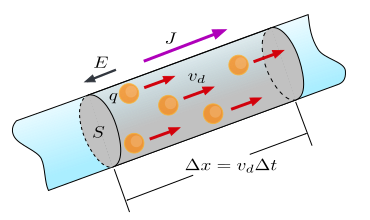
\includegraphics[width=0.5\linewidth]{el_proud_ve_vodici.pdf}
         \caption[Náboje, pohybující se vodičem]{Směr elektrického proudu byl implicitně stanoven
                  jako směr pohybu kladných nábojů. Nositeli elektrického náboje uvnitř vodičů jsou
                  ovšem záporně nabité volné elektrony, které se tedy dle  konvence pohybují proti
                  směru elektrického proudu. Elektrický proud může protékat pevnými látkami (kovy,
                  polovodiči), kapalinami (elektrolyty) a ionizovanými plyny. Látky, které nevedou
                  elektrický proud, nazýváme nevodiči, izolanty}
         \label{TEMP:fig_el_proud_ve_vodici}
      \end{figure}
      
      Elektrický proud je veličina, která obecně popisuje prostorový jev. Omezíme se nyní na běžný
      případ vodiče, jako je na obr. \ref{TEMP:fig_el_proud_ve_vodici}, který má volné náboje jen
      jedné polarity (u kovových vodičů jde o elektrony) a označme $\rho_0$ prostorovou hustotu
      volného náboje a $v_d$ velikost usměrněné rychlosti jejich nositelů (elektronů). Pak za čas
      $dt$ projde průřezem o obsahu $S_0$ ($S_0\bot v_d$) náboj $dQ = \rho_0 S_0 v_d dt$.
      Elektrický proud vyjádřený rov.
      \ref{TEMP:eq_I_01} můžeme přepsat do tvaru
        \begin{equation}\label{TEMP:eq_I_05}
          I = \rho_0 S_0 v_d = - e n_0 S_0 v_d, 
        \end{equation}         
      kde $\displaystyle{n_0 = \frac{\rho_0}{-e}}$ je počet nositelů volného náboje (tj. v našem
      případě elektronů, z nichž každý nese náboj $-e$ v jednotkovém objemu vodiče, přičemž pro
      elektrony zřejmě je $\rho_0<0$.

      \begin{wrapfigure}[14]{r}{5cm}
        \centering
        \includegraphics[width=0.9\linewidth]{plocha_S.pdf}
        \caption[Rovinná plocha $S$.]{Rovinná plocha $S = S_0\cos\alpha$}
        \label{TEMP:fig_plocha_S}
      \end{wrapfigure}
      Rovinnou plochou $S$ průřezu můžeme zavést jako vektor $vr{S}$, který má směr daný normálou k
      ploše a pravidlem pravé ruky (ukazují-li prsty pravé ruky směr oběhu po hraniční křivce
      plochy, ukáže palec směr plochy jako vektoru $\vr{S}$). Protože driftová rychlost $v_d$ je
      také vektor, nebudeme obecně uvažovat vektory $\vr{S}, \vr{v_d}$ o stejném směru a rovnici
      \ref{TEMP:eq_I_05} přepíšeme do obecnějšího tvaru      
      
      \begin{equation}\label{TEMP:eq_I_06}
        I = \rho_0 \vr{S_0}\cdot\vr{v}_d = jS\cos\alpha = jS_0, 
      \end{equation}      
      kde $S_0 = S$ pro $\alpha = 0$ (viz obr. \ref{TEMP:fig_plocha_S}) a   
      \begin{equation}\label{TEMP:eq_I_07}
        \vr{j} = \rho_0\vr{v_d}, 
      \end{equation}        
      je proudová hustota. Je to vektor o velikosti 
      \begin{equation}\label{TEMP:eq_I_08}
        j = \frac{I}{S\cos\alpha} = \frac{I}{S_0}  \qquad A\cdot m^{-2}, 
      \end{equation}   
      obecněji
      \begin{equation}\label{TEMP:eq_I_09}
        j = \frac{dI}{dS}, 
      \end{equation}

      a o směru vektoru driftové rychlosti nositelů kladného náboje. Pro případ nositelů volného
      náboje - elektronů má proudová hustota opačný směr než driftová rychlost $v_d$ (obr.
      \ref{TEMP:fig_plocha_S}).
      
      Velikost vektoru $\vr{j}$ má význam plošné hustoty elektrického proudu v uvažovaném místě
      průřezu. Jednotkou je $A\cdot m^{-2}$.
      
      Nebude-li proudová hustota na uvažovaném průřezu konstantní, bude celkový elektrický proud
      procházející průřezem o obsahu $S$ dán integrálem 
        \begin{equation}\label{TEMP:eq_I_10}
          I = \int_S \vr{j}d\vr{S}. 
        \end{equation} 

      % --------example: Driftová rychlost elektroknů ve vodiči --------
      % \label{TEO:exam008}
      % !TeX spellcheck = cs_CZ
%---------- Driftová rychlost elektroknů ve vodiči: 
\begin{mdframed}[style=mdexam]
\begin{example}\label{TEO:exam008} \emph{Driftová rychlost elektronů ve vodiči:} Vodičem z 
jednomocné mědi o
  průřezu $S_0 = \SI{1}{\mm^2}$ prochází elektrický proud $I = \SI{5}{\A}$. Vypočtěte:
  \begin{itemize}[noitemsep, leftmargin=2em]
    \item počet volných elektronů v jednotkovém objemu \ce{Cu},
    \item úhrnný náboj volných elektronů v jednotkovém objemu,
    \item driftovou rychlost volných elektronů při proudu \(I\).
  \end{itemize}
  Měď má poměrnou atomovou hmotnost $A_r = 63,54$ a hustotu\footnote{Pro hustotu budeme používat 
  alternativní značku $s$, s ohledem na kolizi značky $\rho$, jež označuje hustotu náboje.} $s = 
  \SI{8.93e3}{\kg.\m^{-3}}$.\newline  
  \textbf{Řešení:}
  \begin{itemize}[leftmargin=2em]
    \item Jeden mol mědi o molové hmotnosti $M = \SI{0.06354}{\kg\per\mol}$ a o molovém
          objemu 
          \begin{align*}
            V_m &= \frac{M}{s} 
                 = \frac{\SI{63.54e-3}{\kg.\mol^{-1}}}{\SI{8.93e3}{\kg.\m^{-3}}}      \\
                &= \SI{7.12e-6}{\m^3.\mol^{-1}}
          \end{align*}
          obsahuje $N_A = 6,0221\cdot10^{23}$ jednoatomových molekul \emph{Cu} na jeden mol,
          z nichž každý má volný jeden (valenční) elektron. Tedy počet volných elektronů v
          jednotkovém objemu je 
          \begin{align*}
            n_0 &= \frac{N_A}{V_m} = \frac{sN_A}{M}                                           
                 = \frac{\SI{6.0221e23}{\mol^{-1}}}{\SI{7.12e-6}{\m^{3}.\mol^{-1}}}    \\
                &= \SI{8.46e28}{\per\cubic\m}.
          \end{align*}  
    \item Úhrnný náboj volných elektronů v jednotkovém objemu mědi je 
          \begin{equation}
            Q_v = -e\cdot n_0 = \SI{-1.36e10}{\coulomb.m^{-3}}.
          \end{equation}
    \item Velikost driftové rychlosti určíme ze vztahu $I = -en_0v_dS_0 = - Q_v v_d S_0$ tj.
    \begin{align*}
      v_d &= \left\lvert\frac{I}{Q_v\cdot S_0}\right\rvert                       
           = \frac{\SI{5}{\coulomb\per\s}}{\SI{1.36e10}{\coulomb.m^{-3}}\cdot\SI{1e-6}{\m^2}}   \\
          &= \SI{3676e-4}{\m\per\s} = \SI{0.3676}{\mm\per\s}.  
    \end{align*}
  \end{itemize}
  Z provedených výpočtů si můžeme udělat názor o mikroskopických poměrech v kovových vodičích: počet
  volných nositelů náboje - elektronů a jejich úhrný náboj v jednotkovém objemu je značný a proto
  driftová rychlost elektronů potřebná k vyvolání proudu běžné velikosti v drátových vodičích je
  nesmírně malá (doslova hlemýždí).
\end{example}  
\end{mdframed}
  
      %-----------------------------------------------------------------

      % --------example: Velikost náboje v minci -----------------------
      % \label{TEO:exam009}
      % !TeX spellcheck = cs_CZ
%---------- Velikost náboje v minvi:
\begin{example}
  Elektricky neutrální měděná mince o hmotnosti \(m = \SI{3.11}{\g}\) obsahuje stejné množství 
  kladného a záporného náboje. Jaké je velikost kladného (nebo záporného) náboje obsaženého v 
  minci?\newline  
  \textbf{Řešení:}\newline
  Neutrální atom má záporný náboj \(Z\cdot e\), představovaný jeho elektrony a kladný náboj o 
  stejné velikosti představovaný protony v jádře. Pro měď je atomové číslo \(Z\) rovno \num{29}, 
  tj. atom mědi má \num{29} protonů, a je-li elektricky neutrální, také \num{29} elektronů.
  
  Náboj o velikosti \(Q_v\), který hledáme je roven \(N\cdot Z\cdot e\), kde \(N\) je počet atomů 
  obsažených v  jednom molu (Avogadrova konstanta: \(N_A = \SI{6.0221e23}{\per\mole}\)). Počet 
  molů mědi v minci \(\frac{m}{M}\), kde \(M = \SI{63.5}{\g\per\mole}\) je molární hmotnosti mědi: 
  \begin{equation*}
    N = N_A\cdot\frac{m}{M} = \SI{6.0221e23}{\per\mole}
           \frac{\SI{3.11}{\g}}{\SI{63.5}{\g\per\mole}} 
      = \num{2.95e22}.
  \end{equation*}
 Velikost celkového kladného (záporného) náboje v minci je pak 
  \begin{equation*}
    Q_v = N\cdot Z\cdot e = \num{2.95e22}\cdot\num{29}\cdot\SI{1.602e-19}{\coulomb} 
        = \SI{137039}{\coulomb}
  \end{equation*}
  To je obrovský náboj. Pro srovnání: třeme-li ebonitovou tyč vlněnou látkou, můžeme na tyč 
  přemístit stěží náboj o velikosti \SI{1e-9}{\coulomb}.
\end{example} 
  
      %-----------------------------------------------------------------

    % ----------------Práce a výkon elektrického proudu-----------------
    \subsection{Práce a výkon elektrického proudu}
      % --------example: Ponorný vařič ---------------------------------
      % \label{TEO:exam010}
      % !TeX spellcheck = cs_CZ
%---------- Ponorný vařič:
\begin{mdframed}[style=mdexam]
  \begin{example}\label{TEO:exam010}
    Za jakou dobu uvede norný vodič o příkonu \SI{600}{\W} do varu \SI{1}{\litre} vody o počáteční
    teplotě $\SI{20}{\degreeCelsius}$. Uvažujte měrnou tepelnou kapacitu vody $c =
    \SI{4200}{\joule\per\kg\per\K}$. Výměnu tepla s okolím neuvažujte.
    \newline 
    \textbf{Řešení:}\newline Pro var vody bude zapotřebí tepla dle rovnice $Q  = m\cdot c\cdot(T_2 -
    T_1)$. Potřebná elektrická práce je $Q_e = P\cdot t = U\cdot I\cdot t$ a tedy dobu ohřevu
    stanovíme z rovnice:
    
    {\centering
    \captionsetup{type=figure}
    \luafigure[0.3]{teo_fig033.png}
    \captionof{figure}{Ilustrace k příkladu \ref{TEO:exam010}}
    \label{teo:fig033}
    \par}

    \begin{align*}
      P\cdot t &= m\cdot c\cdot(T_2 - T_1)                                               \\
             t &= \frac{m\cdot c}{P}\cdot(T_2 - T_1)                                     \\     
               &= \frac{\SI{1}{\kg}\cdot\SI{4200}{\joule\per\kg\per\K}}{\SI{600}{\W}}
                \cdot(\SI{100}{\degreeCelsius} - \SI{20}{\degreeCelsius})                \\ 
               &= \SI{560}{\s}.
    \end{align*}         
  \end{example}
\end{mdframed}  
      %-----------------------------------------------------------------
 
    % ----------------Ohmův zákon------------------------------------------------------------------
    \subsection{Ohmův zákon}
      Uvažujme vodič u něhož jsou volnými nositeli náboje \emph{elektrony}. Nyní v mezích klasické
      mechaniky kvantitativně popíšeme mechanismus vedení proudu, který povede k všeobecně známému
      \textbf{Ohmovu zákonu}
      
      Umístíme-li vodič do elektrického pole o intenzitě $\vec{E}$ (např. připojením ke
      galvanickému článku), působí na každý volný elektron síla $\vec{F} = -e\vec{E}$, která mu
      podle \emph{Newtonova zákona} udělí zrychlení $\vec{a} = \frac{\vec{F}}{m_e} = -
      \frac{e}{m_e}\vec{E}$ proti směru vnějšího pole. Tím získávají chaoticky se pohybující
      elektrony ještě složku rychlosti v protisměru vloženého elektrického pole $\vec{E}$ a  dojde
      tedy k usměrnění driftového pohybu volných elektronů a v souladu s kapitolou
      \ref{TEMP:kap_elproud_jev} pozorujeme, že ve vodiči vznikl makroskopický elektrický proud.
      
      Pohyb elektronu se ovšem neobejde bez srážek s ionty v krystalové mřížce. Dráhu, kterou se
      elektronu podaří urazit, nazýváme \emph{volnou dráhou} $d$. Průměrná doba mezi dvěma po sobě
      jdoucími srážkami nechť je $\tau$ za tuto dobu se bude elektron rovnoměrně urychlovat a těsně
      před následující srážkou jeho rychlost dosáhne maxima tj. $\vec{v}_{max} = \vec{a}\cdot\tau$.
      Nás ovšem zajímá průměrná rychlost (\emph{driftová rychlost})na volné dráze průměrné
      velikosti:
      \begin{equation}\label{TEMP:eq_vd_01}
        \vec{v}_d = \frac{\vec{v}_{max}}{2} = -\frac{e\tau}{2m_e}\vec{E}
      \end{equation}   
      Proudová hustota \ref{TEMP:eq_I_07} bude
      \begin{equation}\label{TEMP:eq_j_02}
        \vec{j} = \rho_0\vec{v}_d= -en_0\vec{v}_d = -\frac{e^2n_0\tau}{2m_e}\vec{E}
      \end{equation}       
      Koeficient úměrnosti 
      \begin{equation}\label{TEMP:eq_g_03}
        \gamma = \frac{e^2n_0\tau}{2m_e}
      \end{equation}     
      je závislý na počtů nositelů (elektronů) $n_0$ v jednotkovém objemu a na době $\tau$, neboli
      na délce volné dráhy. Veličina $\gamma$ se nazývá \emph{měrná elektrická vodivost} neboli
      \textbf{konduktivita} látky. Protože dobu $\tau$ nelze přímo měřit, určuje se $\gamma$
      experimentálně. Přitom se zjišťuje, že pro určitou teplotu zkoumané látky je $\gamma$
      konstantní.
      
      Po zavedení pojmu měrná elektrická vodivost látky \ref{TEMP:eq_g_03}, můžeme výraz
      \ref{TEMP:eq_j_02} přepsat do výsledného tvaru
      \begin{equation}\label{TEMP:eq_j_04}
        \vec{j} = \gamma\vec{E},
      \end{equation}              
      který se v literatuře označuje jako \emph{Ohmův zákon v diferenciálním tvaru} (i když se v
      pravém slova smyslu o diferenciální tvar nejedná). Výstižnější je označení \emph{lokální tvar
      Ohmova zákona}, protože výraz \ref{TEMP:eq_j_04} se vztahuje na určité místo, resp. bod,
      vodivého prostředí. Vztah říká, že proudová hustota v určitém bodě vodivého prostředí je
      přímo úměrná intenzitě vloženého elektrického pole v tomto bodě (platí pro určitou teplotu
      prostředí).
      
      Uvažujme nyní lineární homogenní vodič délky $l$ a příčného průřezu o obsahu $S_0$, připojený
      ke zdroji o napětí $U$. Pak intenzita pole uvnitř vodiče bude mít konstantní velikost
      $E=\frac{U}{l}$. Dosadíme-li za velikost proudové hustoty $j=\frac{I}{S_0}$ do
      \ref{TEMP:eq_j_04}, dostaneme vztah
      \begin{equation}\label{TEMP:eq_j_05}
        \frac{I}{S_0} = \gamma\frac{U}{l},
      \end{equation}        
      z něhož vyplývá známý vztah
      \begin{equation}\label{TEMP:eq_j_06}
        U = \frac{l}{\gamma S_0}I = RI,
      \end{equation}              
      kde
      \begin{equation}\label{TEMP:eq_j_07}
        R = \frac{l}{\gamma S_0} = \rho\frac{l}{S_0},
      \end{equation} 
      je \textbf{elektrický odpor} uvažovaného lineárního vodiče, přičemž $\rho = \frac{1}{\gamma}$
      je \emph{měrný elektrický odpor} (\textbf{rezistivita})\footnote{Zde je další kolize značky
      $\rho$. Nyní se tomuto problému vyhneme využíváním pouze konduktivity, jenž se častěji
      používá v teorii elektromagnetického pole.}. Výraz \ref{TEMP:eq_j_07} představuje klasický
      Ohmův zákon zákon experimentálně objevený r. 1826 \emph{G. S. Ohmem}. Jednotky:
      \begin{itemize}\addtolength{\itemsep}{-0.5\baselineskip}
        \item elektrický odpor: \si{V.A^{-1}},
        \item měrný elektrický odpor: \si{\ohm.m},
        \item měrná elektrická vodivost: \si{\ohm^{-1}.m^{-1}}.
      \end{itemize}

      % --------example: Ponorný vařič -----------------------
      % \label{TEO:exam011}
      % !TeX spellcheck = cs_CZ
\begin{example}
  \textbf{Zemnicí elektroda}: Uvažujte zemnicí elektrodu ve tvaru koule o poloměru  
  $a=\SI{200}{\mm}$, uloženou do zeminy v hloubce, která je značně větší než je poloměr $a$. Pro 
  jednoduchost řešení dále předpokládejte, že přívodní drát je od zeminy izolován (obr.
  \ref{TEMP:fig_zem_elektroda}). Zemina má měrnou vodivost $\gamma=\num[exponent-product =
  \cdot]{1,8e-2}\si{\per\ohm\per\m}$. Při zkratu teče přívodním drátem proud $I=\SI{50}{\A}$.
  Vypočítejte:
  
  %----------------------------------
  % image: TEMP_zem_elektroda.tex label: \label{TEMP:fig_zem_elektroda}
  % \documentclass{article}
% \usepackage{tikz}
% \usetikzlibrary{decorations.markings}
% \usetikzlibrary{intersections}
% \usetikzlibrary{calc}

% \begin{document}
   {\centering  
    \begin{tikzpicture}[scale=0.8, every node/.style={scale=1}]
      \coordinate (pCenter) at (0,-5);
      \fill[brown!60] (-2,-0.2) rectangle (2,-7);
      \draw[color=brown, line width=5pt] (-2,-0.2) -- +(4,0); 
      \draw[->,line width=1pt] (0,1) node[left] {$I$} -- (0,-0.1);        
      \draw[line width=1pt] (0,0) -- (pCenter);
      \draw[line width=1pt,color=black, fill=white]
           (pCenter) circle[radius=0.5];
      \draw[line width=1pt, dotted]
           (pCenter) circle[radius=1];
      \foreach \angle in
          {0, 30, 60, 120, 150, 180, 210, 240, 270, 300, 330}
      {
        \draw[->, line width=0.75pt] (pCenter)++(\angle:1.2) -- +(\angle:0.3);        
      }
      \draw[<->, thick] (pCenter)++(240:1) coordinate(pR) -- (pCenter) -- +(330:0.5) coordinate(pA); 
      \node[above] at ($ (pCenter)!0.5!(pA) $) {$a$};     
      \node[above] at ($ (pCenter)!0.9!(pR) $) {$r$}; 
      \node[above] at (-1,-2) {$\gamma$};
      \node[above] at (+1.5,-4.5) {$\vec{j}$};
    \end{tikzpicture}
    \captionsetup{type=figure}
    \captionof{figure}{Zemnicí elektroda}
    \label{TEMP:fig_zem_elektroda}
  \par}
  
% \end{document}    
  %----------------------------------         
  \begin{enumerate}[label=\emph{\alph*})]
    \item Závislost potenciálu $\varphi=\varphi(r)$ elektrického pole, které se vytvoří v
          zemině při zkratu, kde $r$ je vzdálenost od středu elektrody. Potenciál normujte
          volbou $\varphi(\infty)=0$.
    \item Zemnicí odpor elektrody, který je definován vztahem $$R_z=\frac{U_z}{I_z},$$ kde
          $U_z = \varphi(a)-\varphi(b)$ je zemnicí napětí 
    \item Ztrátový výkon při zkratu.            
  \end{enumerate}
  Řešení:    
  Ekvipotenciální a proudové plochy mají zřejmě kulový tvar se středem totožným s geometrickým 
  středem elektrody. Proudová hustota na kulové ploše obecného poloměru $r$ (viz. obr. 
  \ref{TEMP:fig_zem_elektroda}) je $$\vec{j}=\frac{I}{4\pi r^2}\vec{n},$$ kde $\vec{n}$ je 
  jednotkový vektor ve směru normály. Pak v bodech na této ploše musí být elektrické pole o 
  intenzitě $\vec{E}$, kterou určíme ze vztahu
  \begin{equation*}
    \vec{j}= \gamma\vec{E}\rightarrow\vec{E}=
    \frac{\vec{j}}{\gamma}=\frac{I}{4\pi\gamma r^2}\vec{n}.
  \end{equation*}
  Závislost potenciálu $\varphi=\varphi(r)$ tohoto elektrického pole stanovíme pomocí následujícího 
  integrálu
  \begin{equation}
    \varphi = - \int\vec{E}d\vec{r}+C = -\frac{I}{4\pi\gamma}\int\frac{dr}{r^2} + C 
            =   \frac{I}{4\pi\gamma r} + C, \nonumber
  \end{equation} 
  kde integrační konstantu $C$ určíme z okrajové podmínky $\varphi(\infty)=0$, odkud $C=0$.
  Hledaná závislost potenciálu je
  \begin{equation*}
    \varphi = \frac{I}{4\pi\gamma r}, \qquad r\in\langle a, \infty). 
  \end{equation*}           
  
  Zemina, v níž je uložena elektroda, je vlastně rezistorem, jehož jeden okraj tvoří elektrodu
  a druhým okrajem je nekonečně rozlehlý vodivý prostor. Potenciální rozdíl mezi těmito okraji je
  \begin{equation*}
    U_z = \varphi(a) - \varphi(\infty)= \frac{I}{4\pi\gamma a},
  \end{equation*} 
  \begin{minipage}[t]{0.5\textwidth}% first column            
    odkud zemnicí odpor 
    \begin{equation*}
      R_z = \frac{U_z}{I} = \frac{1}{4\pi\gamma a} = \SI{22,1}{\ohm}
    \end{equation*}
  \end{minipage}
  \begin{minipage}[t]{0.5\textwidth}% second column    
    a ztrátový výkon 
    \begin{equation*}
      P_z = R_z\cdot I^2 = \SI{55,3}{\kilo\watt}. 
    \end{equation*}
  \end{minipage}
\end{example}


  
      %-------------------------------------------------------

    % ------------------- Elektromotorické napětí -------------------------------------------------
    \subsection{Elektromotorické napětí}
      Uzavřený proudový okruh $C$, nechť je v dynamické rovnováze - prochází jím ustálený
      elektrický proud. Uvažujme pro jednoduchost představy kladný náboj - ten se musí pohybovat ve
      směru klesajícího potenciálu (záporný náboj ve směru stoupajícího potenciálu). Je-li okruh
      uzavřený, musí kladné náboje opět vystoupit na místo s vyšším potenciálem - musí se tedy
      pohybovat proti elektrostatickým silám. Proto proti úbytku      
               
  % ----------------Stacionární magnetické ole-----------------------------------------------------
  \newpage
  \section{Stacionární magnetické pole}
    Zdrojem stacionárního magnetického pole jsou stejnosměrné proudy nebo permanentní magnety.
    Základní rovnice stacionárního magnetického pole jsou:

    \begin{table}[ht!]
      \centering
      \begin{tabular}{lc|c|}
        \cline{2-3}
        \multicolumn{1}{l|}{} & \textbf{integrální tvar} & \textbf{diferenciální tvar} \\
        \hline
        \multicolumn{1}{|l|}{1. MR} & $\oint\vr{H}\cdot d\vr{l} = I$ & $\rot{H} = \vr{J}$ \\ 
        \cline{1-3}
        \hline
        \multicolumn{1}{|l|}{4. MR} & $\oint\vr{B}\cdot d\vr{S} = 0$ & $\diver{B} = 0$ \\
        \cline{1-3}
        & & $\vr{B} = \mu \vr{H}$ \\
        \cline{3-3}
      \end{tabular}
      \caption{Základní rovnice magnetického stacionárního pole}
    \end{table}

    Směr vektoru $\vr{H}$ se prakticky určí například \emph{pravidlem pravotočivého šroubu}: vodič
    nahradíme šroubem (s pravotočivým závitem) a otáčíme jím tak, aby se pohyboval ve směru proudu;
    směr otáčení pak udává směr vektoru $\vr{H}$. Vše je názorně vysvětleno na obrázku
    \ref{temp:fig_pravidlo_sroub}. Podobných pomůcek existuje více, např. \emph{pravidlo pravé
    ruky}: vodič uchopíme do dlaně pravé ruky tak, aby palec ukazoval směr proudu; prsty pak
    ukazují směr vektoru $\vr{H}$, obr. \ref{temp:fig_pravidlo_ruka}.

         \begin{figure}[ht!]
           \centering
           \subfloat[Pravidlo pravé ruky]{\label{temp:fig_pravidlo_ruka}
             \includegraphics[width=0.4\linewidth]{pravidlo_prave_ruky.pdf}}
           \hspace{2cm}
           \subfloat[Pravidlo pravotočivého šroubu]{\label{temp:fig_pravidlo_sroub}
             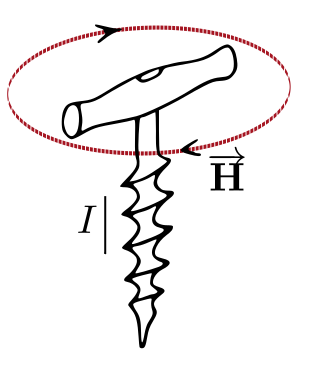
\includegraphics[width=0.3\linewidth]{pravidlo_pravotociveho_sroubu.pdf}}
           \caption[Pravidlo pravé ruku a pravotočivého šroubu]{Určení směru vektoru $\vr{H}$: a)
                   pravidlem pravé ruky; b) pravidlem pravotočivého šroubu}
           \label{temp:fig_urceni_H}
         \end{figure}
    K procvičení těchto pravidel je na obr. \ref{TEMP:fig_ind_c_kruh_z} vyznačen směr indukčních
    čar kruhové\-ho závitu. Označení $\bigotimes$ vyjadřuje proud vstupující  do nákresny (symbol
    letícího šípu od pozorovatele) a označením $\bigodot$ proud vystupující z nákresny (symbol
    hrotu šípu).
    
    \begin{figure}[ht!]
      \centering
      \includegraphics[width=0.4\linewidth]{mag_ind_cary_kruh_z.pdf}
      \caption{Indukční čáry kruhového závitu.}
      \label{TEMP:fig_ind_c_kruh_z}
    \end{figure}    
    Rovnice \ref{TEMP:eq_zak_celk_I} představuje \textbf{zákon celkového proudu} vyjadřující,
    rovnost oběhového magnetické napětí na libovolné uzavřené orientované křivce $c$ proudu, který
    je s křivkou $c$ spřažen. ''\emph{Spřaženým proudem}'' rozumíme proud, který prochází 
    libovolnou plochou $S$, jež je ohraničená křivkou $c$, přičemž plocha $S$ je orientována vůči 
    křivce $c$ pravotočivě (obr. \ref{TEMP:fig_1MR_pic}). \cite[s.~55]{Mayer2001}.

      \begin{equation}\label{TEMP:eq_zak_celk_I}
        \oint\vr{H}\cdot d\vr{l} = I   
      \end{equation}    
     
      \begin{figure}[ht!]
         \centering
         \includegraphics[width=0.7\linewidth]{1MR_pic.pdf}
         \caption[Zákon celkového proudu]{K zákonu celkového proudu}
         \label{TEMP:fig_1MR_pic}
      \end{figure}

         \begin{figure}[hb!]
           \centering
           \subfloat[$\oint\vr{H}\cdot d\vr{l} = 0$]{\label{TEMP:fig_mag_sprazeny_proud1}
             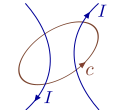
\includegraphics[width=0.3\linewidth]{mag_sprazeny_proud1.pdf}}
           \subfloat[$\oint\vr{H}\cdot d\vr{l} = 0$]{\label{TEMP:fig_mag_sprazeny_proud2}
             \includegraphics[width=0.3\linewidth]{mag_sprazeny_proud2.pdf}}
           \subfloat[$\oint\vr{H}\cdot d\vr{l} = 3I$]{\label{TEMP:fig_mag_sprazeny_proud3}
             \includegraphics[width=0.3\linewidth]{mag_sprazeny_proud3.pdf}}             
           \caption[K pojmu ''proud spřažený s křivkoku'']{K pojmu ''proud spřažený s křivkoku''
                    pro tři různé případy křivky $c$.}
           \label{TEMP:fig_mag_sprazeny_proud123}
         \end{figure}
         
    Základní úlohou řešení stacionárních proudových magnetických polí je určení rozložení veličin 
    $\vr{H}$ a $\vr{B}$ v prostoru, je-li dáno prostorové a materiálové uspořádání a elektrické 
    proudy vybuzují řešené magnetické pole.
    
    V následujících úlohách se omezíme na analýzu jednodušších, souměrných magnetických polí v 
    lineárním izotropním alespoň po částech homogenním prostředí. Pro zjednodušení budeme 
    zanedbávat deformaci magnetického pole v okrajových oblastech a nebudeme uvažovat vliv 
    blízkosti nesymetrického rozhraní a vliv blízkosti druhého zdroje magnetického pole. (Pro 
    přesnější řešení by pak bylo nutné použít tzv. \emph{metodu zrcadlení}.) Některá složitější 
    pole lze rozdělit na několik jednodušších polí souměrného charakteru, resp. typického 
    uspořádání. Vzhledem k tomu, že v předpokládaném lineárním prostředí ($\mu 
    = konst$) platí pro stacionární magnetické pole \emph{princip superpozice}, lze samostatně 
    vyřešit nejprve dílčí jednodušší pole jednotlivých proudů $I_j$ a po jejich superpozici
      \begin{equation}\label{TEMP:eq_superp_mag_pole}
        \vr{H}= \sum_{j=1}^n\vr{H}_j(I_j), \quad\text{resp.}\quad \vr{B}= 
        \sum_{j=1}^n\vr{B}_j(I_j)   
      \end{equation}
    získáme výsledné pole celkového proudu \cite[s.~181]{Kotlan1999}. 
    
    Metodou přímé aplikace I. Maxwellovy rovnice v integrálním tvaru pro stacionární magnetické
    pole proudové
      \begin{equation}\label{TEMP:eq_1MR_rozbor}
        \oint_\mathcal{C}\vr{H}d\vr{l} = \oint_\mathcal{C}H\cos\alpha dl = I_c
      \end{equation}    
    lze jednoduše použít tehdy, je-li ze zadané úlohy zřejmá taková symetrie pole, že lze z 
    nekonečně mnoha uzavřených křivek, splňující rov. \ref{TEMP:eq_1MR_rozbor}, nalézt takovou 
    integrační dráhu $c$, která obepíná proud $I_c$ vytvářející magnetické pole a v jejichž bodech 
    platí podmínka
      \begin{equation}\label{TEMP:eq_H_alpha_konst}
        H = \text{konst}, \qquad \alpha = \text{konst},
      \end{equation}    
    speciálně
      \begin{equation}\label{TEMP:eq_alpha_0}
        H = \text{konst}, \qquad \alpha = 0.
      \end{equation}
    
    Podmínka $\alpha = 0$, tj. $\vr{H}\| d\vr{l}$ je identicky splněna na siločáře magnetického 
    pole. Siločáry souměrných stacionárních magnetických polí splňují tedy podmínku 
    \ref{TEMP:eq_alpha_0} a řešení rovnice \ref{TEMP:eq_1MR_rozbor} při integraci po takovéto 
    siločáře je jednoduché
      \begin{equation}\label{TEMP:eq_1MR_alpha0}
        \oint_\mathcal{C}\vr{H}d\vr{l} = H\underbrace{\oint_\mathcal{C} dl}_{l_c} = 
                                         I_c \rightarrow H = \frac{I_c}{l_c}
      \end{equation}            
    kde $l_c$ je délka integrační dráhy $c$ splňující podmínku \ref{TEMP:eq_alpha_0}.
      
    Klasickým případem takovéto úlohy je magnetické pole \emph{dlouhého přímého válcového vodiče} o
    poloměru $a$, délky $l$ protékaného proudem $I$ rozloženým po průřezu souměrně kolem osy 
    vodiče, tzn, obecně s hustotou $J = J(r)$. Z osové (rotační) symetrie vyplývá, že siločáry 
    magnetického pole mají tvar soustředných kružnic se středem v ose vodiče, ležících v rovině 
    kolmé na osu vodiče obr. \ref{TEMP:fig_mag_pole_vodic_I_konst}.
    \begin{figure}[ht!]
      \centering
      \includegraphics[width=0.7\linewidth]{mag_pole_vodic_I_konst.pdf}
      \caption[Pole dlouhého dutého vodiče protékaného konstantním proudem]{Pole dlouhého dutého
               vodiče protékaného konstantním proudem}
      \label{TEMP:fig_mag_pole_vodic_I_konst}
    \end{figure}        
    Úlohy proto řešíme ve válcových souřadnicích s osou $z$ totožnou s osou vodiče. Za 
    předpokladu, že průměr vodiče je zanedbatelný vůči jeho délce lze zanedbat deformaci pole 
    vlivem konců válcového vodiče a přejít na rovinný problém v polárních souřadnicích. Z důvodu 
    osové  souměrnosti je však pole závislé jen na vzdálenosti $r$ od osy vodiče tj. $$H = H(r), 
    \qquad B = B(r).$$ Na kruhových siločárách je tedy splněna podmínka \ref{TEMP:eq_alpha_0} a z 
    I. Maxwellovy rovnice \ref{TEMP:eq_1MR_rozbor} 
      \begin{equation}\label{TEMP:eq_1MR_rozbor2}
        \oint_{\mathcal{C}}\vr{H}d\vr{l} = H\cos0\oint_\mathcal{C}dl = I(r),
      \end{equation}     
    kde $c$ je kružnice o poloměru $r$ a proud $I(r)$ je dán rovnicí
      \begin{equation}\label{TEMP:eq_1MR_Ir}
        I(r) = \int_{S(r)}\vr{J}(r)d\vr{S} = \int_0^rJ(r)2\pi rdr
      \end{equation}           
    je proud protékající přes kruhovou plochu $S(r)$ ohraničenou kružnicí o poloměru $r$. Pak
    intenzita magnetického pole ve vzdálenosti $r$ od osy vodiče má velikost
      \begin{equation}\label{TEMP:eq_Hr_vodice}
        H = H(r) = \frac{I(r)}{2\pi r},
      \end{equation}       
    a magnetická indukce 
      \begin{equation}\label{TEMP:eq_Br_vodice}
        B = B(r) = \frac{\mu I(r)}{2\pi r},
      \end{equation}       
    přičemž $\mu$ je \emph{permeabilita} v bodech na poloměru $r$. Magnetické pole v okolí
    kruhové\-ho přímého vodiče protékaného proudem $I$ viz obr. \ref{teo:fig021} je tedy v souladu 
    s předchozími úvahami dáno výrazy \cite[s.~183 - 185]{Kotlan1999}:
    \begin{figure}[ht!]
      \centering
      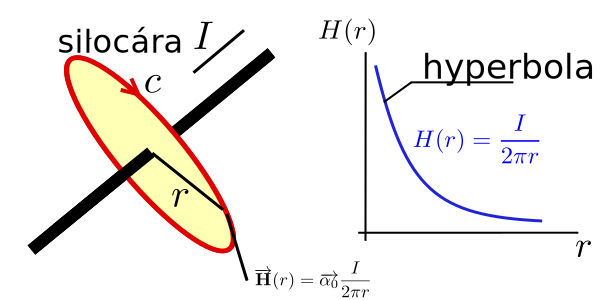
\includegraphics[width=0.8\linewidth]{teo_fig021.pdf}
      \caption[Průběh intenzity magnetického pole dlouhého dutého vodiče protékaného konstantním
               proudem]{Průběh intenzity magnetického pole dlouhého dutého vodiče protékaného
               konstantním proudem}
      \label{teo:fig021}
    \end{figure}      
      \begin{equation}\label{TEMP:eq_Hr_Br_vodice}
        H = H(r) = \frac{I}{2\pi r}, \qquad B = B(r) = \frac{\mu I}{2\pi r}.
      \end{equation}   
    Jelikož 1. MR má nenulovou pravou stranu v magnetickém poli obecně není splněna nutná a
    postačující podmínka, aby magnetické napětí
      \begin{equation}\label{TEMP:eq_mag_napeti}
        \int_{M(l)}^N\vr{H}d\vr{l} = U_{m_{MN}} \qquad [A]
      \end{equation}       
    nezáviselo na tvaru integrační cesty $l$ z $M$ do $N$. Tedy obecně nelze zavést \emph{skalární
    magnetický potenciál}. Magnetické pole je tedy obecně \textbf{vírové (nepotenciální)}.

    Všimněme si však speciálních případů, kdy pravá strana 1. MR je nulová a tedy magnetické pole
    bude \textbf{nevírové (magnetostatické)}. K tomu dochází buď v oblasti kde 
      \begin{equation}\label{TEMP:eq_1MR_0}
        \oint_{\mathcal{C}}\vr{H}d\vr{l} = 0
      \end{equation}    
    tj. takové v němž neexistuje uzavřená křivka $c$ spřažená s nějakým proudem, nebo v takovém
    bodu, v němž platí
      \begin{equation}\label{TEMP:eq_rotH_0}
        \rot{\vr{H}} = 0
      \end{equation}
    tj. v bodu v němž je $\vr{J} = 0$.
    
    Analogicky jako v elektrostatice, lze pak zavést magnetický potenciál $\varphi_m$ vztahem  
      \begin{equation}\label{TEMP:eq_grad_varphi_m}
        \vr{H} = - \grad{\varphi_m}.
      \end{equation}              
    Jednotkou $\varphi_m$ je \emph{ampér} [A]. Pro magnetické napětí mezi body $M, N$ platí
    analogicky
      \begin{equation}\label{TEMP:eq_Umn_def}
        U_{MN} = \int_{M(l)}^N\vr{H}d\vr{l} = \varphi_m(M) - \varphi_m(N),
      \end{equation}        
    nezávisle na integrační cestě $l$. 
     
    % ----------------Magnetické pole vodičů s proudem v homogenním izotropním prostředí ----------
    \subsection{Magnetické pole vodičů s proudem v homogen\-ním izo\-trop\-ním prostředí}
      Z předchozí kapitoly vyplývá, že intenzitu magnetického pole $\vr{H}$ lze stanovit pomocí
      vztahu $\oint\vr{H}\cdot d\vr{l} = I$ tehdy, víme-li předem, že daným bodem prochází silová
      čára, na níž je intenzita pole konstantní, $H_s = \text{konst}$. V tomto případě se křikový
      integrál změní v pouhý součin intenzity pole a délky silové čáry
       
       \begin{equation}\label{TEMP:eq_1MR_v_hom_p}
         \oint_\mathcal{C}\vr{H}d\vr{l} = H_s\oint_\mathcal{C}\vr{l} = H_s\cdot l_s
       \end{equation}      
       
      takže lze vypočítat intenzitu pole $$H_s = \frac{I}{l_s}$$ pro body silové čary. 
      
      Tohoto postupu lze použít i tam, kde uvedená podmínka není splněna, avšak pole lze vyjádřit
      superpozicí dílčích polí, z nich každé tuto podmínku splňuje, viz příklad 
      \ref{TEMP:ex_koax_H}. 

      % --------example: $H=f(r)$ dlouhého dutého válcového vodiče ------
      % \label{TEO:exam012}
      % !TeX spellcheck = cs_CZ
\begin{example}
  Stanovte intenzitu magnetického pole $H=f(r)$ dlouhého dutého válcového vodiče podle obr.
  \ref{TEMP:fig_pole_duty_valec} při rovnoměrném rozložení proudu $I$ po průřezu. 
  
   {\centering
    \captionsetup{type=figure}
    \includegraphics[width=0.6\linewidth]{duf_duty_valec_H.pdf}
    \captionof{figure}{K příkladu stanovení intenzity magnetického pole dlouhého dutého válcového 
               vodiče protékaného proudem}
    \label{TEMP:fig_pole_duty_valec}
  \par}
  
  Vodič s rovnoměrně rozloženým proudem podle obr. \ref{TEMP:fig_pole_duty_valec} je rotačně
  souměrný podle své osy a tedy i jeho magnetické pole je souměrné. Silové čáry jsou soustředné
  kružnice, vektor $\vr{H}$, jenž má směr tečny ke kružnici, je po celé délce kružnice stejně
  velký. Lze tedy snadno použít integrálního tvaru 1. MR (\textbf{zákon celkového proudu})
  
  Pro body ležící vně vodiče obepíná kruhová integrační dráha (vedená po silové čáře 1) celý
  proud vodiče $I$ a platí
  \begin{equation}\label{TEMP:eq_1MR_duty_valec}
    \oint_\mathcal{C}\vr{H}d\vr{l} = H\cdot 2\pi r = I
  \end{equation}
  takže intenzita pole je
  \begin{equation}\label{TEMP:eq_H_duty_valec}
    H = \frac{I}{2\pi r}
  \end{equation}
  
  Ve stěně dutého magnetického vodiče jsou silové čáry rovněž kružnice, neboť magnetické pole
  je i zde souměrné. Tyto siločáry však obepínají jen část proudu $I'$ vodiče pro oběh siločáry
  2 platí
  \begin{equation}\label{TEMP:eq_1MR_uvnitr_valce}
    \oint_\mathcal{C}\vr{H}d\vr{l} = H\cdot 2\pi r = I' = \pi(r^2-r_1^2)J
  \end{equation}
  kde $J$ je hustota proudu ve vodiči
  \begin{equation}\label{TEMP:eq_J_duty_valec}
    J = \frac{I}{S}= \frac{I}{\pi(r_2^2-r_1^2)}
  \end{equation}
  Ve stěně vodiče je tedy intenzita pole
  \begin{equation}\label{TEMP:eq_H_uvnitr_valce}
    H = \frac{I}{2\pi r}\frac{r^2-r_1^2}{r_2^2-r_1^2}
  \end{equation}
  V dutině vodiče je intenzita rovna nule. Vzhledem k souměrnosti pole by i zde muselo platit
  $\oint_\mathcal{C}\vr{H}d\vr{l} = H\cdot 2\pi r$. Protože dráha s poloměrem $r<r_1$ neobepíná
  žádný proud, je $\oint_\mathcal{C}\vr{H}d\vr{l} = 0$ a tedy musí byt $H = 0$.
\end{example}    
  
      %------------------------------------------------------------------

      % --------example: $H=f(r)$ souosého kabelu -----------------------
      % \label{TEO:exam013}
      % !TeX spellcheck = cs_CZ
\begin{mdframed}[style=mdexam]
  \begin{example}\label{TEMP:ex_koax_H}
    Stanovte intenzitu magnetického pole dlouhého přímého souosého kabelu podle obr.
    \ref{teo:fig066}. Středním vodičem (\emph{žílou}) prochází proud $I$ a týž proud
    opačného smyslu prochází vnějším vodičem (\emph{pláštěm}). Proudy jsou rovnoměrně rozloženy po
    průřezech vodičů. Nakreslete graf průběhu $H = f(r)$ \cite[s.~92]{Dufek1970},
    \cite[s.~195]{Kotlan1999}.
    
    {\centering
    \luafigure[0.45]{teo_fig066a.pdf}     \hspace{1em}
    \luafigure[0.45]{teo_fig066b.pdf}
    \captionsetup{type=figure}  
    \captionof{figure}{K příkladu stanovení intenzity magnetického pole dlouhého souosého kabelu
      protékaného proudem: a) náčrt; b) $H=f(r)$}           
    \label{teo:fig066}
    \par}
 
    \textbf{Řešení}: \newline Rovnici \ref{TEMP:eq_1MR_v_hom_p} aplikujeme na jednotlivé intervaly
    osově souměrného stacionárního magnetického pole, přičemž se prakticky jedná o superpozici dvou
    polí. V oblasti $r<r_2$ se uplatňuje pouze pole vnitřního válcového vodiče (žíly), pro $r>r_2$
    přistupuje souosé pole vnějšího trubkového vodiče.
    \begin{itemize}
      \item Pro oblast $r<r_1$ je vzhledem k 
            \begin{align*}
                % \nonumber to remove numbering (before each equation)
                \dd{I}&= \vr{J}d\vr{S} \\
                I(r)  &= \int_S dI = \int_S \vr{J}d\vr{S} = \int_S J\cos\beta dS \\
                      &= \left\lvert\begin{array}{cc}
                                \beta = 0 & H = \text{konst}   \\
                              S = \pi r^2 & dS = 2\pi r\dd{r}  \\
                              \end{array}
                        \right\rvert                                           \\
                      &= J\int_0^r 2\pi rdr = J\pi r^2
            \end{align*}
            hledané řešení 1. MR dáno 
            $$\oint_{\mathcal{c}}\vr{H}d\vr{l} = H_1 2\pi r = I(r) = J\pi r^2$$ kde celková proudová
            hustota je  $$J = \frac{I}{\pi r_1^2}$$ a tedy
            $$H_1 = \frac{I}{2\pi r_1^2}\cdot r$$
            
      \item Pro oblast $r_2>r>r_1$ řešíme v podstatě pole vně osamoceného válcového vodiče $I(r)$ a
            tedy $$H_2 = \frac{I}{2\pi r}$$
      \item Pro $r>r_3$ je magnetické pole vytvářeno celým proudem žíly $I$ a příslušnou částí
            proudu pláště $J\pi(r^2 - r_2^2)$, kde proudová hustota $$J =
            \frac{I}{\pi(r_3^2-r_2^2)}$$ má opačnou orientaci oproti proudové hustotě žíly. Pak 
            \begin{align*}
              I(r)                             &= I - I\frac{r^2-r_2^2}{r_3^2-r_2^2} \\
              \oint_{\mathcal{c}}\vr{H}d\vr{l} &= H_32\pi r = I(r)                   \\          
              H_3                              &= \frac{I}{2\pi r}\left(1 - 
              \frac{r^2 - r_2^2}{r_3^2 - r_2^2}\right) 
            \end{align*}
            Stejný výsledek dostaneme superpozicí opačně orientovaných polí
            $$H_3 = H'_3 - H''_3 = \frac{I}{2\pi r} - \frac{I}{2\pi r}\left(\frac{r^2 - r_2^2}{r_3^2
            - r_2^2}\right)$$. 
    \end{itemize}
    Průběh $H(r)$ je na obr. \ref{teo:fig066}.
  \end{example}
\end{mdframed}  
      %------------------------------------------------------------------

    % -----------Magnetické pole elektrického proudu v diferenciálním tvaru-----------------------
    \subsection{Magnetické pole elektrického proudu v diferenciálním tvaru}
      Nechť je opět magnetické pole vyvoláno konstantním el. proudem $I = \text{konst}$. Jak
      vyplývá z předchozí kapitoly, základním vztahem pro toto pole je \emph{Ampérův zákon}
      $$\oint_\mathcal{c}\vr{H_c}d\vr{l} = I$$  Zvolme za integrační dráhu $c$ obvod malé plošky
      $\Delta S$, jíž prochází proud $\Delta I = J_n \Delta S$, kde $J_n$ je průmět vektoru hustoty
      proudu do směru normály plošky $\Delta S$ (předpokládáme, že ploška $\Delta S$ je dostatečně
      malá, aby se dalo počítat s konstantní hustotou proudu v celém jejím rozsahu)
      \cite[s.~13]{Trnka1972}. Pro zvolený případ platí
      
      \begin{equation}\label{TEMP:eq_amp_z1}
        \oint_\mathcal{c}\vr{H_c}d\vr{l}  =
           J_n \Delta S \rightarrow \frac{1}{\Delta S}\oint_\mathcal{c}\vr{H_c}d\vr{l} = J_n
      \end{equation} 
      
      Pro $\Delta S \rightarrow 0$ zavedeme označení 
      \begin{equation}\label{TEMP:eq_amp_z2}
        \rot{H}  = \frac{1}{\Delta S}\oint_\mathcal{c}\vr{H_c}d\vr{l}  = J_n
      \end{equation}
      
      Rovnice \ref{TEMP:eq_amp_z2} říká, že \emph{rotace vektoru} $\vr{H}$, ($\rot{H}$), jehož
      průmět do určitého směru je roven průmětu vektoru hustoty proudu do tohoto směřu. Z uvedených
      vztahu je patrný fyzikální význam rotace vektoru $\vr{H}$. Je to vektor, jehož velikost je
      rovna oběhovému magnetickému napětí po dráze v rovině kolmé k vektoru hustoty proudu,
      vztaženém k ploše obepínané oběhovou drahou (v nehomogenní poli to platí pro případ, že se
      plocha dráhy blíží k nule).
      
      Při použití pravoúhlé soustavy kartézských souřadnic $x$, $y$ a $z$ jsou průměty vektoru
      $\rot{H}$ do jednotlivých os
      \begin{equation}\label{TEMP:eq_amp_z3}
        \textsf{rot}_x\mathbf{H} = J_x, \qquad 
        \textsf{rot}_y\mathbf{H} = J_y, \qquad
        \textsf{rot}_z\mathbf{H} = J_z
      \end{equation}      
      Průmět $\textsf{rot}_x\mathbf{H}$ je dán oběhovým magnetickým napětím po obvodu plošky $dydz$
      a platí
      \begin{align}\label{TEMP:eq_amp_z4}
        \textsf{rot}_x\mathbf{H} 
          &= \frac{1}{dydz}\oint_\mathcal{c}\vr{H_c}d\vr{l}                   \nonumber \\
          &= \frac{1}{dydz}\left[H_ydy + 
                           \left(H_z + \pder{Hz}{y}dy\right)dz\right] -       \nonumber \\
          &- \frac{1}{dydz}\left[\left(H_y - 
                           \pder{Hy}{z}dz\right)dy - H_zdz\right]             \nonumber \\
          &= \frac{1}{dydz}\left[\pder{Hz}{y}dydz - \pder{Hy}{z}dydz\right]   \nonumber \\
          &= \pder{Hz}{y} - \pder{Hy}{z} = J_z
      \end{align}       
      
      \begin{figure}[ht!]
        \centering
        \includegraphics[width=0.65\linewidth]{rotH_dxdy.pdf}
        \caption[K odvození pojmu $\textsf{rot}_z\mathbf{H}$]{K odvození pojmu
                 $\textsf{rot}_z\mathbf{H}$}
        \label{TEMP:fig_rotH_dxdy}
      \end{figure}            
      tedy dostáváme
      \begin{align}\label{TEMP:eq_amp_z5}
        \textsf{rot}_x\mathbf{H} &= \pder{H_z}{y} - \pder{H_y}{z} = J_x       \nonumber \\
        \textsf{rot}_x\mathbf{H} &= \pder{H_x}{z} - \pder{H_z}{x} = J_y       \nonumber \\
        \textsf{rot}_x\mathbf{H} &= \pder{H_y}{x} - \pder{H_x}{y} = J_z            
      \end{align}        
      Pro \emph{pravoúhlé souřadnice} $x, y, z$ můžeme tedy vztah $\rot{H} = \vr{J}$ rozepsat na
      tvar
      \begin{equation*} % \label{TEMP:eq_amp_z6}
        \textsf{rot}\mathbf{H} 
           = \vr{i}\,\textsf{rot}_x\mathbf{H} + 
             \vr{j}\,\textsf{rot}_y\mathbf{H} +
             \vr{k}\,\textsf{rot}_z\mathbf{H}
     \end{equation*}
     \begin{align*}
         \.&= \vr{i}\left(\pder{H_z}{y} - \pder{H_y}{z}\right) +  
             \vr{j}\left(\pder{H_x}{z} - \pder{H_z}{x}\right) +
             \vr{k}\left(\pder{H_y}{x} - \pder{H_x}{y}\right)                 \\  
         \.&= \vr{i}\,J_x + \vr{j}\,J_y + \vr{k}\,J_z = \vr{J}.
      \end{align*}          
      
      Rotaci vektoru $\rot{H}$ můžeme též symbolicky vyjádřit vektorovým součinem Hamiltonova
      operátoru a vektoru $\vr{H}$
      \begin{align*} %\label{TEMP:eq_amp_z7}
        \rot{H}  &= \nabla\times\vr{H}                                                      \\
                 &= \left(\vr{i}\,\pder{ }{x} + 
                   \vr{j}\,\pder{ }{y} + \vr{k}\,\pder{ }{z}\right)\times(\vr{i}\,H_x +
                   \vr{j}\,H_y + \vr{k}\,H_z)
      \end{align*}
      nebo také determinantu
      \begin{equation}\label{TEMP:eq_amp_z8}
        \rot{H} = \begin{vmatrix}
                    \vr{i}       & \vr{j}      & \vr{k}      \\
                    \pder{ }{x}  & \pder{ }{y} & \pder{ }{z} \\ 
                    H_x          & H_y         & H_z         \\
                  \end{vmatrix}      
      \end{equation}  
      \emph{cylindrických souřadnic} $r$, $\varphi$, $z$:
      \begin{align}\label{TEMP:eq_amp_z9}
        \textsf{rot}_r\mathbf{H}       
          &= \frac{1}{r}\pder{H_z}{\varphi} - \pder{H_\varphi}{z} = J_r           \nonumber \\ 
        \textsf{rot}_\varphi\mathbf{H} 
          &= \pder{H_r}{z} - \pder{H_z}{r}                        = J_\varphi     \nonumber \\
        \textsf{rot}_z\mathbf{H}       
          &= \frac{1}{r}\left[\pder{ }{r}
             \left(rH_\varphi\right)-\pder{H_r}{\varphi}\right]   = J_z
      \end{align} 
      \emph{sférických souřadnic} $r$, $\varphi$, $\vartheta$ 
      \begin{align}\label{TEMP:eq_amp_z10}
        \textsf{rot}_r\mathbf{H}        
           &= \frac{1}{r\sin\vartheta}\left[\pder{ }{\vartheta}(H_\varphi\sin\vartheta) - 
              \pder{H_\vartheta}{\varphi}\right]                     = J_r           \nonumber \\ 
        \textsf{rot}_\varphi\mathbf{H}   
           &= \frac{1}{r}\left[\pder{ }{r}(rH_\vartheta) - 
              \pder{H_r}{\vartheta}\right]                           = J_\varphi     \nonumber \\
        \textsf{rot}_\vartheta\mathbf{H} 
           &= \frac{1}{r\sin\vartheta}\left[\pder{H_r}{\varphi} -
              \pder{ }{r}\left(rH_\varphi\sin\vartheta\right)\right] = J_\vartheta    
    \end{align} 
      Podobně jako v elektrickém poli vyjadřujeme vztah $\oint\vr{D}d\vr{S} = Q$ vztahem $\diver{D}
      = \rho$, tak i v magnetickém poli vyjadřujeme vztah $\oint\vr{B}d\vr{S} = 0$ vztahem
      $\diver{D} = 0$, nebo též v kartézských souřadnicích $x$, $y$ a $z$ jako $$\diver{D} =
      \nabla\cdot\vr{B} = \pder{B_x}{x} + \pder{B_y}{y} + \pder{B_z}{z} = 0$$
                     
    % ----------------Rovnice pro magnetický potenciál -------------------------------------------
    \subsection{Rovnice pro magnetický potenciál}
      V regulárních bodech lineárního homogenního izotropního magnetika platí pro $\varphi_m$
      \textbf{Laplaceova rovnice}
      \begin{equation}\label{TEMP:eq_varphi_m_laplace}
        \Delta\varphi_m = 0
      \end{equation}      
      Důkaz plyne z rovnice $\diver{B} = 0$ a rovnice $\vec{B} = \mu\vec{H}$: $$\diver{B} =
      \textsf{div}\mu\vec{H} = \textsf{div}\mu(-\textsf{grad}\varphi_m).$$ Pro $\mu = \text{konst}$
      dostáváme $\textsf{div}\textsf{grad}\varphi_m = 0$, což je rovnice
      \ref{TEMP:eq_varphi_m_laplace}.
      
      Na rozhraní mezi dvěma magneticky různými prostředími neplatí Maxwellovy rovnice v
      diferenciálním tvaru a tedy ani Laplaceova rovnice \ref{TEMP:eq_varphi_m_laplace}. Podmínky 
      pro $\vr{H}$ a $\vr{B}$ na rozhraní vyjádříme pomocí skalárního magnetického potenciálu
       \begin{align}\label{TEMP:eq_mag_U_rozhrani}
         \varphi_{m1}                 &= \varphi_{m2} \\
         \mu_1\pder{\varphi_{m1}}{n}  &= \mu_2\pder{\varphi_{m2}}{n} 
       \end{align}
      kde $\pder{}{n}$ jsou derivace ve směru normály k rozhraní. 
    
    \subsubsection{Vektorový magnetický potenciál}
      V elektrostatice jsme pro usnadnění mnohých problémů zavedli skalární elektrický potenciál -
      lze jej zavést vždy, neboť elektrostatické pole je vždy potenciální. Magnetické pole je však
      obecně vírové. Lze jej popsat skalárním potenciálem jen ve speciálních případech, tj.
      jestliže je polem potenciálním. Obecně je však zavedení skalárního potenciálu nepřípustné.
      Lze i pak zavést nějakou veličinu (analogickou skalárnímu potenciálu), s níž by se pracovalo
      snáze, než přímo s vektory pole?
      
      Dříve než definujeme vektorový magnetický potenciál, zopakujme zavedení skalárního potenciálu
      v elektrostatice. Vyjdeme z 2. MR a z rovnice známé z vektorové analýzy: $$\rot{E} = 0 \qquad
      \text{a} \qquad \textsf{rot}\,\textsf{grad}\varphi_m = 0.$$
      
      V magnetickém poli vyjdeme ze 4. MR a z jiné identity pro vektorovou funkci $\vr{A}$, známe z
      vektorové analýzy: $$\diver{B} = 0 \qquad \text{a} \qquad \textsf{div}\textsf{rot}\vec{A} =
      0$$ odtud
        \begin{equation}\label{TEMP:eq_B_rotA}
          \vec{B} = \rot{A}.
        \end{equation}       
               
%} % tikzset
%~~~~~~~~~~~~~~~~~~~~~~~~~~~~~~~~~~~~~~~~~~~~~~~~~~~~~~~~~~~~~~~~~~~~~~~~~~~~~~~~~~~~~~~~~~~~~~~~~~
\printbibliography[title={Seznam literatury}, heading=subbibliography]
\addcontentsline{toc}{section}{Seznam literatury}
  % \input{../src/TEO/chap/teo1ch02.tex} 
}{ % DEBUG was off
\LuaPartBckgrnd{titleBG_fractal1.png}
\LuaPartTitle{TEO}{Teorie elektrických obvodů}{TEO}
\parttoc
%========== Kapitola: Základy elektrických obvodů =================================================
  % !TeX spellcheck = cs_CZ
%file:intro_TEO.tex
{\tikzset{external/prefix={tikz/TEO/}}
 \tikzset{external/figure name/.add={ch09_}{}}
%================================= Kapitola: Základy elektrických obvodů ===========================
\chapter{Základy elektrických obvodů}
\minitoc

  \section{Struktura elektrických ob\-vo\-dů}
    Ke každému skutečnému, fyzicky realizovanému, elektrickému obvodu lze nakreslit 
    \textbf{obvodové schéma}. Toto schéma je vlastně \emph{obvodovým modelem} skutečného obvodu. 
    Obvodový model je sestaven ze základních obvodových prvků - \textbf{dvojpólů}. Název plyne z 
    důležité topologické vlastnosti dvojpólů - mají dvě svorky \cite[s.~12]{Patocka2}.
    
    \subsection{Teorie elektromagnetického pole a elektrické obvody}
      Uspokojivý výklad všech makroskopických elektromagnetických jevů, jež probíhají v 
      nepohyblivých látkových prostředích, poskytuje Maxwellova klasická teorie elektromagnetického 
      pole. Vyšetření elektromagnetického pole (tj. určení vektorů \(\vec{E}\) a \(\vec{B}\) ve 
      všech bodech zkoumané oblasti pro každý okamžik) lze vždy provést integrací Maxwellových 
      rovnic pro dané okrajové a počáteční podmínky. Rovnice elektromagnetického pole se mohou 
      mnohdy zjednodušit, např. zanedbáním Maxwellova („posuvného“) proudu proti proudu vodivému v 
      1. Maxwellově rovnici u kvazistacionárních magnetických polí, zjednodušením geometrické 
      konfigurace apod. Přesto však řada technických úloh vede k dosti náročným matematickým 
      problémům. V některých případech však lze dosáhnout \emph{podstatného zjednodušení} řešení 
      použitím metod teorie elektrických obvodů. Teorie elektromagnetického pole tím sice nepozbývá 
      svůj základní význam pro elektrotechniku, avšak teorie elektrických obvodů umožňuje 
      efektivnější koncepci řešení některých technických úloh.
      
      Přistoupíme k vysvětlení pojmu \textbf{elektrický obvod}. Různá elektrotechnická zařízení lze 
      často považovat za systém složený z jednoduchých částí rozmanitě mezi sebou spojených, jimiž 
      mohou procházet proudy. Dále budeme předpokládat, že elektromagnetické jevy v tomto systému 
      lze vyjádřit pomocí \emph{napětí a proudů}. (Nebudeme tedy používat veličin \(\vec{E}\); 
      \(\vec{B}\); \(\vec{D}\); \(\vec{H}\), jež lokálně charakterizují elektromagnetické pole.) 
      Takový systém nazýváme \emph{reálným elektrickým obvodem}. Při studiu reálného elektrického 
      obvodu se abstrahujeme od jeho nepodstatných vlastností a omezujeme se jen na ty, jež jsou 
      pro zkoumaný jev rozhodující. Touto idealizací přecházíme k jednoduššímu systému, který 
      obecně nazýváme \emph{modelem}. Modelem může být opět reálný elektrický obvod, který zkoumáme 
      \emph{experimentálně}, zde však budeme mít na zřeteli pouze abstraktní modely, které 
      vyšetřujeme teoreticky. Tyto modely, jejichž vlastnosti budeme dále zkoumat, nazýváme 
      \emph{ideálními elektrickými obvody} anebo krátce \emph{obvody}\cite[s.~19]{Meyer1978}.
      
      Sestavení obvodu, jenž dostatečně přesně vystihuje reálný elektrický obvod v jeho provozních 
      podmínkách, není předmětem teorie obvodů, nýbrž disciplín, které teorii obvodů používají 
      (např. teorie elektrických strojů, elektroenergetiky, radiotechniky, sdělovací 
      elektrotechniky). \emph{Teorie obvodů vychází z těchto modelů a zkoumá jejich vlastnosti a 
      metody řešení}, která zpravidla mají vysoký stupeň přesnosti. Naproti tomu při sestavení 
      obvodu bychom se mohli dopustit chyby, kdybychom jej neověřovali konfrontací jeho vlastností 
      s originálem. Jelikož obvod nevyjadřuje všechny vlastnosti reálného elektrického obvodu, 
      vznikají jisté rozpory mezi teorií obvodů a Maxwellovou teorií elektromagnetického pole. 
      Například v teorii obvodů se předpokládá, že elektrická energie se přenáší vodiči obvodu — 
      lze ji snadno určit z napětí a proudů těchto vodičů. Naproti tomu z Maxwellovy teorie plyne, 
      že se veškerá energie přenáší dielektrikem v okolí vodičů; vodiče pouze určují směr toku této 
      energie. Tyto rozpory však nejsou překážkou pro používání teorie obvodů v praxi.
      
      %----------------------------------
      % image: \ref{TEO:fig_dvojpol}
      \begin{wrapfigure}{r}{5cm}
  \centering
  \begin{tikzpicture}[scale=1,>=latex']
     \filldraw[fill=green!20!white, draw=green!50!black, very thick] (-1,1) rectangle (1,0);
     \coordinate (v1) at (-2,0.5);
     \coordinate (v2) at (-1,0.5);
     \coordinate (v3) at (1,0.5);
     \coordinate (v4) at (2,0.5);
     \draw[-o] (v2) -- (v1);
     \draw[-o] (v3) -- (v4); 
  \end{tikzpicture}
  \caption{Dvojpól}
  \label{TEO:fig_dvojpol}
\end{wrapfigure}  
      %----------------------------------
      Libovolnou část obvodu, která je vyvedena k jedné dvojici svorek, nazýváme 
      \textbf{dvojpólem}; jeho schematické označení je na obr. \ref{TEO:fig_dvojpol}. Veličinu, jež 
      fyzikálně charakterizuje dvojpól, nazýváme jeho parametrem. Dvojpóly, které lze 
      charakterizovat jediným reálným parametrem, nazýváme \textbf{ideálními prvky obvodu} anebo 
      krátce \emph{prvky obvodu}.
      
      Z Maxwellovy teorie plyne, že elektromagnetické vlnění vyvolané elektromagnetickými jevy v 
      obvodu se šíří prostorem rychlostí světla. Pro jednoduchost předpokládejme, že 
      elektromagnetická vlna má harmonický průběh. Jsou-li geometrické rozměry reálného 
      elektrického obvodu zanedbatelně malé ve srovnání s délkou elektromagnetického vlnění, lze 
      rychlost jeho šíření považovat za nekonečně velkou a geometrické rozměry reálného 
      elektrického obvodu se neuplatní — napětí a proudy v tomto obvodu jsou pak pouze funkcí času 
      t. Lze jej modelovat obvodem, jehož magnetické pole je \emph{kvazistacionámi}; parametry jeho 
      dvojpólů nejsou funkcemi geometrických souřadnic. Hovoříme o \emph{obvodu se soustředěnými 
      parametry}.
      
      Nejsou-li geometrické rozměry reálného elektrického obvodu zanedbatelné vzhledem k délce 
      elektromagnetické vlny, je nutné brát v úvahu konečnou rychlost šíření elektromagnetického 
      vlnění — napětí a proudy v tomto obvodu pak budou nejen funkcemi času \(t\), ale též polohy v 
      prostoru, určené souřadnicemi \(x, y, z\) (zpravidla postačí jediná souřadnice). Parametry 
      dvojpólů takového obvodu jsou též funkcemi polohy, a proto hovoříme o \emph{obvodu s 
      rozprostřenými (rozloženými) parametry}.
            
      Teorie obvodů je úzce spjata s kybernetikou, a proto jsou některé pojmy těchto vědních oborů 
      společné. Jak známo, kybernetika se zabývá studiem \emph{systémů libovolné povahy, které jsou 
      schopny přijímat, uschovávat a zpracovávat informaci a využívat ji k řízení}. Obvod je 
      speciálním případem systému, v němž dochází k interakci s okolím na \emph{vstupu (na 
      vstupních svorkách)} a na \emph{výstupu (na výstupních svorkách)}; na vstup jsou připojeny 
      \emph{zdroje energie}, na výstup \emph{spotřebiče}. Napětí a proudy na vstupu představují 
      \emph{podněty (stimuly)} čili \emph{vstupní veličiny}, na výstupu představují \emph{odezvy 
      (reakce)} čili \emph{výstupní veličiny}.
      
      Základními vlastnostmi obvodu jsou: \emph{chování obvodu}, tj. závislost mezi podněty a 
      odezvami a \emph{struktura obvodu}, tj. vlastnosti jeho prvků a způsob jejich spojení. 
      Strukturu obvodu charakterizují jednak fyzikální vlastnosti prvků tvořících obvod, jednak 
      způsob jejich vzájemného spojení. V prvém případě hovoříme o \emph{fyzikální struktuře} 
      obvodu, ve druhém o jeho \emph{topologické (geometrické) struktuře}\cite[s.~21]{Meyer1978}.
      
      
    \subsection{Fyzikální struktura obvodů} 
      \subsubsection{Uzly a větve obvodu, orientace větví, větvové proudy a 
      napětí}\label{TEO:chap_Term}
        Místo styku dvou nebo několika svorek prvků obvodu nazýváme \emph{uzlem obvodu}. Dvojpól 
        spojující dvojici uzlů nazýváme \emph{větví obvodu}. Větve obvodu orientujeme, jestliže 
        jeden z uzlů větve zvolíme za počáteční a druhý za koncový. Větve obvodu lze orientovat 
        libovolně, avšak pro pevně zvolený časový okamžik \(t\). Protože směry proudů ve větvích se 
        mohou s časem měnit, nemusí se v obecném okamžiku \(t\) shodovat orientace větví se směry 
        proudů ve větvích. Pro obvody se soustředěnými parametry a se zavedenou orientací větví 
        definujeme: \emph{Okamžitou hodnotou větvového proudu} \(i\) budeme nazývat okamžitou 
        hodnotu proudu procházejícího průřezem větve, jehož orientace (směr normály) je dána 
        orientací větve. Z této definice plyne, že okamžitá hodnota větvového proudu je kladná v 
        čase \(t\), kdy je směr proudu ve větvi souhlasný s orientací větve a záporná pro ta \(t\), 
        kdy je směr proudu opačný. Okamžitý směr proudu budeme ve schématech vyznačovat šipkou 
        \begin{tikzpicture}\draw[-open triangle 45] (0,0) -- (1,0);\end{tikzpicture} podle obr. 
        \ref{TEO:fig_dvojpol_iu}.
        
        \begin{figure}
          \centering
          \begin{tikzpicture}[scale=1]
   \filldraw[fill=green!20!white, draw=green!50!black, very thick] (-1,1) rectangle (1,0);
   \coordinate (v1) at (-2,0.5);
   \coordinate (v2) at (-1,0.5);
   \coordinate (v3) at (1,0.5);
   \coordinate (v4) at (2,0.5);
   \draw[-o] (v2) -- (v1);
   \draw[-o] (v3) -- (v4); 
   \draw[-open triangle 45] (1.2,0.8) -- (1.8,0.8) node[right] {\(i\)};
   \draw[-triangle 45] (v1) ++ (0.2,-0.2) to [out=-45,in=-135] (1.8,0.4);
   \node[below] at (0,-0.4) {\(u\)};
\end{tikzpicture}
          \caption{Větvový proud \(i\), větvové napětí \(u\) a orientace větve}
          \label{TEO:fig_dvojpol_iu}
        \end{figure}

        \emph{Okamžitou hodnotou větvového napětí} u budeme nazývat okamžitou hodnotu napětí mezi 
        počátečním a koncovým uzlem orientované větve v daném čase \(t\). Orientaci větvového 
        napětí budeme ve schématech vyznačovat šipkou 
        \begin{tikzpicture}\draw[-triangle 45] (0,0) to (1,0);\end{tikzpicture} podle obr. 
        \ref{TEO:fig_dvojpol_iu}, přičemž šipka směřuje od počátečního ke koncovému uzlu 
        orientované dráhy, po níž se napětí měří.
        
      \subsubsection{Ideální prvky obvodu a jejich chování}
        Ideální prvky jsou z hlediska svých fyzikálních vlastností i matematického popisu 
        nejjednoduššími dvojpóly obvodu. O vodičích, které je spojují, předpokládáme, že mají 
        nulový odpor a že průchodem proudu nevzniká v jejich okolí magnetické pole. Elektrické 
        pole, jež je obecně vírové, je vně každého prvku obvodu polem potenciálním. Z toho plyne, 
        že hodnota napětí mezi dvojicemi uzlů obvodu nezávisí na tvaru integrační dráhy (tj. na 
        uspořádání přívodů voltmetru) mezi těmito uzly.
        
        Ideální prvky obvodu dělíme na aktivní a pasívní.
        
        \textbf{Aktivní prvky} jsou zdroje elektrické energie (generátory). Zpravidla přijímají 
        neelektrickou formu energie (např. mechanickou, chemickou, tepelnou) a přeměňují ji na 
        elektrickou energii, kterou dodávají do obvodu. Rozlišujeme dva typy aktivních prvků:
        \begin{itemize}
          \item ideální zdroje napětí obr. 5a), jejichž jediným parametrem je svorkové napětí     
                \(u_0 =  u_0(t)\)
          \item ideální zdroje proudu obr. 5b), jejichž jediným parametrem je dodávaný proud      
                \(i_0 = i_0(t)\)
        \end{itemize}
        
        Napětím ideálního napěťového zdroje rozumíme okamžitou hodnotu napětí mezi svorkami zdroje 
        v pořadí, jež stanovíme tím, že první svorku označíme znakem + a druhou znakem —. Svorky 
        zdroje tedy tvoří uspořádanou dvojici: svorka + se bere jako první a svorka — jako druhá. U 
        zdrojů časově proměnného napětí nemusejí znaky + a — představovat skutečnou polaritu 
        svorek; jsou to referenční znaky, jež pouze vyjadřují, že udávané napětí je měřeno od 
        svorky označené + ke svorce označené —. Skutečnou polaritu svorek vyjadřují v těch 
        okamžicích, v nichž je \(u_0(t) > 0\).
        
        V teorii obvodů se ideální zdroje dělí dále na \emph{nezávislé (autonomní)} a na 
        \emph{řízené (závislé, neautonomní)}.
        \begin{itemize}
          \item \textbf{Nezávislý ideální zdroj napětí} má svorkové napětí \(u_0 = u_0(t)\) 
                nezávislé na zatížení zdroje (tj. na výkonu dodávaném zdrojem do obvodu).
          \item \textbf{Nezávislý ideální zdroj proudu} dodává do obvodu proud \(i_0 = i_0(t)\) 
                nezávislý na zatížení zdroje.
          \item \textbf{Řízený ideální zdroj napětí, řízený napětím}, má svorkové napětí, jež je 
                funkcí napětí na některé části obvodu.
          \item \textbf{Řízený ideální zdroj napětí}, řízený proudem, má svorkové napětí, jež je 
                funkcí proudu v některé části obvodu.
          \item \textbf{Řízený ideální zdroj proudu}, řízený napětím, dodává proud, jenž je funkcí 
                napětí v některé části obvodu.
          \item \textbf{Řízený ideální zdroj proudu}, řízený proudem, dodává proud, jenž je funkcí 
                proudu v některé části obvodu.
        \end{itemize}
        
        S řízenými zdroji se často setkáváme v elektronice. Například zesilovač napětí lze nahradit 
        řízeným ideálním zdrojem napětí, přičemž napětí zdroje je funkcí napětí nebo proudu 
        přiváděného na vstup zesilovače.

        \emph{Základních obvodových prvků} je celkem pět: rezistor, cívka, kondenzátor, ideální 
        zdroj napětí, ideální zdroj proudu. Zdůrazněme následující skutečnosti:
        \begin{itemize}
          \itemsep0em 
          \item Každý ze základních prvků je uvažován jako \textbf{ideální} (nemá žádné jiné  
                parazitní vlastnosti).
          \item Kombinací základních prvků vznikne \textbf{náhradní zapojení} skutečného prvku, 
                včetně jeho parazitních vlastností.
          \item Z pěti základních prvků je tedy možno sestavit \textbf{libovolný obvodový model}
                (elektrický obvod) \textbf{pasivní} i \textbf{aktivní}.
          \item U \textbf{aktivních obvodů} (např. zesilovačů) se uplatňují řiditelné, neboli
                parametrické prvky. Typickým příkladem je bipolární tranzistor, jenž je řízen 
                proudem do báze.
        \end{itemize}
      
      \subsubsection{Přizpůsobení zdroje a spotřebiče}
        Zajímavé je sledovat, jak se mění napětí, proud a výkon na spotřebiči v závislosti na 
        poměru odporu spotřebiče a vnitřního odporu zdroje. Jednoduchou úvahou lze usoudit, že 
        největší napětí je naprázdno při nekonečném odporu spotřebiče a největší proud bude při 
        nulovém odporu spotřebiče (zkratu). Maximum výkonu nebude ani při maximálním proudu, 
        protože napětí na zkratu je nulové, ani při maximálním napětí, protože obvodem neprotéká 
        proud. Výkon, který je součinem napětí a proudu, je v obou případech nulový.
        
        Pokud připojíme k náhradnímu napěťovému schématu zdroje spotřebič, bude pro protékající 
        proud platit: \(I = \frac{U_i}{R_i + R_z}\). Po dosazení vztahu pro napětí na spotřebiči, 
        které je shodné se svorkovým napětím zdroje \(U=I\cdot R_z\), získáme vztah: \(U = 
        U_i\frac{R_z}{R_i + R_z}\).
        
  \section{Topologická struktura obvodů}
    Topologické vlastnosti obvodů lze studovat pomocí teorie grafů, jež je odvětvím 
    topologie\footnote{Topologie je moderní	matematická disciplína zabývající se studiem takových 
    vlastností objektů, jež jsou invariantní vzhledem k vzájemně jednoznačnému spojitému zobrazení, 
    jehož inverzní zobrazení je též spojité. Tyto vlastnosti se nazývají topologické vlastnosti 
    (topologické invarianty). (Zmíněné zobrazení lze názorně interpretovat jako takové deformování 
    zkoumaného objektu, při němž se nesmí objekt porušit ani spojovat.) Například hovoříme-li o 
    topologických vlastnostech obvodů, nemáme na mysli způsob rozmístění prvků obvodu v prostoru, 
    nýbrž počet prvků a vlastnosti jejich vzájemného spojení. Studium topologických vlastností 
    obvodů spadá do odvětví topologie, zvaného teorie grafů. Základy teorie grafů byly vybudovány 
    právě na základě potřeb teorie obvodů (G. Kirchhoff).}
    
    \subsection{Základní pojmy z topologie obvodů}
      Definice grafu obvodu. Mějme v prostoru body \(B_1; B_2;\cdots; B_{n_u}\) — nazveme je uzly. 
      Dvojice těchto uzlů nechť tvoří krajní body navzájem se neprotínajících oblouků (tzv. 
      topologických úseček) \(v_1; v_2; \cdots; v_{n_v}\) — nazveme je \emph{větvemi}. Množinu 
      všech větví pak nazýváme \emph{grafem obvodu}.
      
      Graf obvodu tedy vyjadřuje topologickou strukturu obvodu a získáme jej tím, že jej 
      abstrahujeme od fyzikálních vlastností prvků obvodu. U grafu nás nezajímají jeho metrické 
      vlastnosti, tj. uzly grafu lze libovolně rozmístit a jeho větve lze libovolně deformovat, 
      avšak nesmíme je přerušit a po jejich deformaci je popřípadě opět spojit.
      
      Graf, který vznikne z grafu \(\mathscr{G}\) těmito úpravami, nazýváme \emph{izomorfním} (čili 
      \emph{topologicky ekvivalentním}) s grafem \(\mathscr{G}\). Na obr. \ref{TEO:fig_topo01} je 
      příklad obvodu a jeho tří izomorfních grafů.
      
      \begin{figure}[ht!]
        \centering
        \includegraphics[width=0.9\linewidth]{TEO_topo01.jpg}
        \caption{ Obvod (a) a jeho topologicky ekvivalentní (izomorfní) grafy (b), (c), (d) 
                  \cite[s.~39]{Meyer1978}}
        \label{TEO:fig_topo01}
      \end{figure}
      
      Uzly grafu jsou charakterizovány svým stupněm: \emph{stupeň uzlu} \(\varepsilon\) udává počet 
      větví grafu, jež s uvažovaným uzlem \emph{incidují}\footnote{Dva geometrické útvary nazýváme 
      \textbf{incidentní} (resp. říkáme, že spolu incidují), jestliže jeden z nich obsahuje útvar 
      druhý. Například všechny přímky procházející daným bodem jsou s ním incidentní, nebo všechny 
      křivky ležící na ploše s ní incidují.}. Uzel stupně \(0\) (tzv. \emph{izolovaný uzel}) a uzel 
      stupně \(1\) (větev s ním incidující se nazývá \emph{izolovaná}) mají význam v matematické 
      teorii grafů, ale v grafech obvodů se setkáváme jen s uzly stupně \(\varepsilon\geqq 2\). 
      Někdy je výhodné vypustit uzly stupně \(2\) (tzv. vnitřní uzly větví) a uvažovat jen uzly 
      stupně \(\varepsilon\geqq 3\). Tím zmenšíme počet větví obvodu, avšak v jeho větvích obecně 
      nebude již jediný prvek, ale složitější dvojpól — sériové spojení prvků; např. v grafu obvodu 
      na obr. \ref{TEO:fig_topo01} jsou uzly \(B_1; B_2; B_3; B_4\) vesměs 3. stupně, uzly \(B_5; 
      B_6\) jsou 2. stupně vnitřní uzly); graf má \(n_v = 8\) větví. Omezíme-li se na uzly stupně 
      \(\varepsilon\geqq 3\), představují větve \(v_3; v4\) jedinou větev s krajními uzly \(B_2; 
      B_3\) a podobně větve \(v_7; v_6\) tvoří jedinou větev s uzly \(B_2; B_4\) graf má pak jen 
      \(n_v = 6\) větví.
      
      Dvojici grafů, jejichž izomorfismus je porušován jen uzly 2. stupně, nazýváme 
      \emph{homeomorfními}. Homeomorfní grafy jsou tedy takové grafy, jež se po odstraněni 
      některých uzlů 2. stupně stanou izomorfními.
  
  \section{Kirchhoffovy zákony}
    V této kapitole budeme formulovat Kirchhoffovy zákony a ukážeme, jak lze jejich použitím popsat 
    chováni obvodu soustavou rovnic.
    
    \subsection{Formulace prvního a druhého Kirchhoffova zákona}
      Kirchhoffovy zákony, spolu se vztahy mezi napětími a proudy pasivních prvků (tab. 3), mají 
      pro teorii obvodů základní význam. \emph{Platí pro jakýkoliv obvod se soustředěnými 
      parametry}, lineární i nelineární, s parametry časově konstantními i s časově proměnnými. Z 
      hlediska teorie obvodů lze Kirchhoffovy zákony považovat za postuláty, z nichž tato teorie 
      vychází. Z hlediska teorie elektromagnetického pole jsou však důsledkem plynoucím z 
      Maxwellovy teorie.
      
%     \begin{mdframed}[style=MyFrame]
      \textbf{První Kirchhoffův zákon}. Pro libovolný uzel obvodu platí: Součet okamžitých hodnot 
      proudů vystupujících z uzlu a proudů vstupujících do uzlu je roven nule. Přitom proudy 
      vystupující z uzlu bereme jako kladné a proudy vstupující do uzlu jako záporné.
%     \end{mdframed} 
      
      \begin{proof}
        Uvažujme libovolný uzel obvodu \(B_j\). Obklopíme jej libovolnou uzavřenou orientovanou 
        plochou \(S\) obr. \ref{TEO:fig_KZ01}a). Vzhledem k tomu, že magnetické pole obvodu se 
        soustředěnými parametry je kvazistacionární, má rovnice kontinuity tvar
        \begin{equation}
          \oint_s \vec{J}(t)\dd{\vec{S}} = 0
        \end{equation}
        \begin{figure}[ht!]
          \centering
          \includegraphics[width=0.9\linewidth]{TEO_KZ01.jpg}
          \caption{Uzel incidující s pěti větvemi: reálný elektrický obvod (a) a ideální obvod (b). 
                   (K odvozeni prvního Kirchhoffova zákona) \cite[s.~47]{Meyer1978}}
          \label{TEO:fig_KZ01}
        \end{figure}      
        Pro tok vektoru proudové hustoty uzavřenou plochou \(S\) podle obr. \ref{TEO:fig_KZ01}a) 
        platí
        \begin{equation}
          \oint_s \vec{J}(t)\dd{\vec{S}} = \sum_{\mathclap{\substack{k\\B_j\in v_k}}}
                                           \int_{S_k} \vec{J}(t)\dd{\vec{S}} 
        \end{equation}
        kde sumace na pravé straně rovnice je provedena přes indexy všech větví incidujících s 
        uzlem \(B_j\). Jednotliví sčítanci představují proudy vystupující z uzlu, resp. vstupující 
        do uzlu. Porovnáním obou uvedených vztahů plyne dokazovaný první Kirchhoffův zákon.
      \end{proof}
      
      Matematicky lze zapsat první Kirchhoffův zákon pro libovolný uzel obvodu \(B_j\) pomocí 
      větvových proudů \(i_k\) libovolně orientovaných větví \(v_k\)\footnote{Orientace větví 
      obvodu je libovolná, ale pevně zvolená (nezávislá na čase), viz kap. \ref{TEO:chap_Term}.} ve 
      tvaru 
      \cite[s.~47]{Meyer1978}
      \begin{equation}\label{TEO:eq_KZI}
        \sum_{\mathclap{\substack{k\\B_j\in v_k}}} \pm i_k = 0; \qquad j = 1;\ldots; n_u 
      \end{equation}
      Znaménko \(+\) platí, je-li větev \(v_k\) orientována tak, že uzel \(B_j\) je jejím 
      počátečním uzlem a znaménko \(—\) platí v opačném případě; sčítáme pro všechna \(k\), pro něž 
      uzel \(B_j\) inciduje s větví \(v_k (B_j\in v_k)\); \(n_u\) je počet všech uzlů obvodu. 
      Poznamenejme, že podle definice větvového proudu (viz kap. \ref{TEO:chap_Term}) je \(i_k > 
      0\), souhlasí-li směr proudu s orientaci větve a \(i_k < 0\) v opačném případě.
      
      Například pro uzel \(B_2\) podle obr. \ref{TEO:fig_KZ01}b) má první Kirchhoffův zákon tvar
      \begin{equation*}
        -i_1 - i_3 - i_4 + i_7 + i_8 = 0
      \end{equation*}
      Rovnice (\ref{TEO:eq_KZI}) je symbolickým zápisem prvního Kirchhoffova zákona, vyžadujícím 
      slovní komentář o tom, kdy máme brát znaménko \(+\) , kdy znaménko \(—\) a jakých hodnot 
      nabývá sčítací index \(k\). Tento zápis prvního Kirchhoffova zákona je velmi dobře použitelný 
      pro řešení jednodušších obvodů. Naproti tomu při řešení obvodů na počítači je třeba vyjádřit 
      první Kirchhoffův zákon výstižnějším zápisem ve tvaru
      \begin{equation}\label{TEO:eq_KZI_01}
        \sum\limits_{k=1}^{n_v} a_{jk} i_k = 0; \qquad j = 1;\ldots; n_u 
      \end{equation}
      \begin{figure}[ht!]
        \centering
        \includegraphics[width=0.9\linewidth]{TEO_KZ02.jpg}
        \caption{K určení hodnot koeficientů \(a_{jk}\) \cite[s.~47]{Meyer1978}}
        \label{TEO:fig_KZ02}
      \end{figure}
      kde koeficienty \(a_{jk}\) vyjadřují incidenci uzlů a větví v orientovaném grafu obvodu a 
      nabývají těchto hodnot: \(a_{jk} = 1\), když j-tý uzel je počátečním uzlem k-té větve, 
      \(a_{jk} = — 1\), když j-tý uzel je koncovým uzlem k-té větve a \(a_{jk} = 0\), když j-tý 
      uzel neinciduje s k-tou větví (obr. \ref{TEO:fig_KZ02}). Znaménko větvového proudu \(i_k\) 
      plyne ze souhlasnosti, resp. nesouhlasnosti orientace větve a směru větvového proudu (\(i_k > 
      0\), resp. \(i_k < 0\)).
      
      \textbf{Druhý Kirchhoffů v zákon}. Pro libovolnou orientovanou smyčku obvodu platí: Součet 
      okamžitých hodnot napětí na všech větvích incidujících s orientovanou smyčkou obvodu je roven 
      nule. Přitom napětí větví bereme jako kladná, jestliže proud ve větvi v daném okamžiku 
      prochází ve smyslu orientace smyčky a jako záporná, jestliže prochází v opačném směru.
      
      \begin{proof}
        Uvažujme libovolnou orientovanou uzavřenou křivku \(s_j\) procházející všemi uzly smyčky 
        obvodu a vedenou vně prvků (např. křivku vyznačenou na obr. \ref{TEO:fig_KZ03} tečkovaní). 
        Z vlastností ideálních prvků obvodu plyne, že II. Maxwellova rovnice v integrálním tvaru má 
        pro křivku \(s_j\) tvar
        \begin{align}
          \oint\vec{E}\dd{\vec{l}} &= 0    \label{TEO:eq_KZ01} \\
          \shortintertext{Pro oběhové napětí po křivce \(s_j\) (obr. \ref{TEO:fig_KZ03}) zároveň 
                          platí vztah}
          \oint\vec{E}\dd{\vec{l}} &= \sum_{\mathclap{\substack{k\\v_k\in s_j}}}\vec{E}\dd{\vec{l}}
        \end{align}
        Porovnáním obou uvedených vztahů plyne dokazovaný druhý Kirchhoffův zákon.
        \begin{figure}[ht!]
          \centering
          \includegraphics[width=0.7\linewidth]{TEO_KZ03.jpg}
          \caption{Smyčka incidující se šesti větvemi (K odvození druhého Kirchhoffova 
                   zákona)\cite[s.~48]{Meyer1978}}
          \label{TEO:fig_KZ03}
        \end{figure}
      \end{proof}
      Matematicky lze vyjádřit druhý Kirchhoffův zákon pro libovolnou orientovanou smyčku \(s_j\) 
      pomocí větvových napětí \(u_k\) libovolně orientovaných větví \(v_k\) ve tvaru
      \begin{equation}\label{TEO:eq_KZ03}
        \sum_{\mathclap{\substack{k\\v_k\in s_j}}} \pm u_k = 0 \qquad j=1;\cdots; n_s
      \end{equation}
      Znaménko \(+\) platí, je-li větev \(v_k\) orientována souhlasně se smyčkou \(s_j\) a znaménko 
      \(—\) platí v opačném případě; sčítáme pro všechna \(k\), pro něž větev \(v_k\) inciduje se 
      smyčkou \(s_j (v_k\in s_j)\); \(n_s\) je počet všech smyček obvodu.
      
      Například pro smyčku \(s_4\) podle obr. \ref{TEO:fig_KZ03} má druhý Kirchhoffův zákon tvar
      \begin{equation*}
        -u_2 -u_4 -u_5 +u_6 +u_7 -u_8 = 0
      \end{equation*}
      
      Vyjádření druhého Kirchhoffova zákona rovnicí (\ref{TEO:eq_KZ03}) je — obdobně jako vyjádření 
      prvního Kirchhoffova zákona rovnicí (\ref{TEO:eq_KZI}) — jen symbolickým zápisem, k němuž 
      bylo nutno připojit slovní komentář. Pro řešení obvodů na počítači je třeba vyjádřit druhý 
      Kirchhoffův zákon matematicky výstižnějším zápisem
      \begin{equation}\label{TEO:eq_KZ04}
        \sum\limits_{k=1}^{n_v} b_{jk} u_k = 0 \qquad j=1;\cdots; n_s
      \end{equation}      
      \begin{figure}[ht!]
        \centering
        \includegraphics[width=0.9\linewidth]{TEO_KZ04.jpg}
        \caption{K určení koeficientů \(b_{jk}\) \cite[s.~49]{Meyer1978}}
        \label{TEO:fig_KZ04}
      \end{figure}      
      kde koeficienty \(b_{jk}\) vyjadřují incidenci smyček a větví v orientovaném grafu obvodu a 
      nabývají těchto hodnot: \(b_{jk} = 1\), když \(k\)-tá větev inciduje s \(j\)-tou smyčkou a 
      orientace obou se shodují, \(b_{jk} = — 1\), když \(k\)-tá větev inciduje s \(j\)-tou smyčkou 
      a orientace obou je opačná, a \(b_{jk} = 0\), když \(k\)-tá větev neinciduje s \(j\)-tou 
      smyčkou (obr. \ref{TEO:fig_KZ04}).
      
  \section{Analýza elektrických obvodů}
    Pojem \textbf{analýza} není v teorii elektrických obvodů používán v původním širokém smyslu. 
    Zejména v souvislosti s počítačovým řešením obvodů se pod analýzou obvykle rozumí 
    \emph{konkrétní metody získávání elektrických charakteristik obvodů z jejich modelů} (například 
    kmitočtová nebo stejnosměrná analýza).
    
    \subsection{Modelování, analýza, simulace}
      \emph{Analýzu} provádíme ve snaze získat informace o určitých vlastnostech zkoumaného obvodu, 
      které nás zajímají. Z praktických důvodů však zpravidla analýze nepodrobujeme samotný obvod, 
      nýbrž jeho \emph{model}. Jedním z dobrých důvodů může být skutečnost, že daný obvod dosud 
      existuje pouze v představě návrháře a před jeho výrobou je vhodné ověřit, zda je navržen 
      správně. K modelování obvodu máme k dispozici elementární modely elektrických prvků (pasivní 
      R, L, C, tranzistory, operační zesilovače apod.) ve formě matematického popisu jejich 
      fungování a  jejich elektrotechnických značek, které jsou začleněny do schématu celkového 
      zapojení. Z hlediska matematického je model obvodu představován soustavou rovnic, které lze 
      odvodit na základě rovnic dílčích elektrických prvků a Kirchhoffových rovnic, které 
      reprezentují způsob propojení součástek \cite[s.~16]{Biolek}.
      
      Při modelování obvodu je důležité nejprve uvážit, s jak složitým modelem bude vhodné 
      pracovat. Složité modely obvykle umožňují věrnější popis chování skutečného obvodu, avšak 
      současně prudce rostou požadavky na výkon analyzačního nástroje. Je zřejmé, že výpočty, které 
      provádíme jen pomocí papíru a tužky, případně kalkulačky, jsou vhodné pro analýzu méně 
      rozsáhlých obvodů s jednoduchými modely, kde nám jde buď o ověření správnosti základního 
      principu fungování, nebo o odhady chování obvodu s odhlédnutím od různých parazitních jevů a 
      vlivů reálných vlastností součástek na vlastnosti obvodu. Složité modely si můžeme dovolit 
      používat při analýze s využitím speciálních počítačových programů.

      Klasická teorie obvodů dává odpověď na otázku, s jakým minimálním počtem typů elementárních 
      modelů obvodových prvků je možné sestavit model jakkoliv složitého analogového obvodu se 
      soustředěnými parametry: jsou to pasivní prvky typu R,L,C a zdroje klasické a řízené. 
      Příslušné charakteristiky těchto prvků jsou popsány jednoduchými nebo složitými rovnicemi. Z 
      tohoto pohledu můžeme říci, že k sestavování modelů daných obvodů a k jejich využívání nemáme 
      k dispozici nic jiného než omezený počet modelů elementárních prvků s příslušnými 
      matematickými vzorci \cite[s.~17]{Biolek}.
      
      Od jisté úrovně modelování, která zajišťuje uspokojivou shodu chování modelu a originálu, je 
      možné model využívat k simulaci skutečného chování obvodu za konkrétních podmínek. Příkladem 
      může být sledování vlivu teploty na nastavený stejnosměrný pracovní bod tranzistorového 
      zesilovače. Dostáváme se k poslednímu pojmu z trojlístku \emph{modelování - analýza - 
      simulace}. Simulace je tedy něco více než analýza (v úzkém pojetí) a analýza je důležitá 
      součást simulace.
      
      \begin{figure}[ht!]
        \centering
        \includegraphics[width=0.95\linewidth]{Biolek_Modelovani.jpg}
        \caption{Modelováni, analýza, simulace \cite[s.~17]{Biolek}}
        \label{TEO:fig_modelovani}
      \end{figure}
      
      Shrnutí:
      \begin{itemize}
        \itemsep0em
        \item \emph{Při řešení obvodu pomocí „papíru, tužky a kalkulačky“} nejprve sestavíme model 
              obvodu ve formě schématu zapojení včetně parametrů, resp. charakteristik jednotlivých 
              součástek. Z tohoto modelu pak vzniká model matematický ve formě rovnic, které 
              vyplývají z vzájemného propojení a vlastností součástek, Kirchhoffových zákonů a 
              Ohmová zákona. Tento model pak podrobíme numerické analýze.      
        \item \emph{Při řešení pomocí počítačového programu} opět sestavujeme model obvodu,  
              většinou pomocí schematického editoru. Program je však schopen při tomto sestavování 
              účinně pomáhat tím, že je zdrojem složitých interních modelů součástek (tranzistory, 
              operační zesilovače, integrované obvody...). Vlastní sestavení rovnic, jejich řešení 
              a vizualizace výsledků je již plně v režii programu \cite[s.~18]{Biolek}.
      \end{itemize}
      
    \subsection{Metody analýzy heuristické a algoritmické}
      Metodu analýzy můžeme chápat jako konkrétní postup od modelu obvodu až po získání cíle analýzy.
      
      Všechny existující metody analýzy můžeme rozdělit na \emph{nealgoritmické (heuristické)} a 
      \emph{algoritmické}. Do první kategorie patří postupy, které řešitel volí na základě svých 
      předchozích zkušeností s využíváním tvůrčího přístupu. Například při výpočtu napětí na 
      výstupu zatíženého děliče napětí je možno nejprve sloučením zatěžovacího a pracovního 
      rezistoru převést řešení na problém děliče nezatíženého, posléze vypočítat proud děličem a 
      následně výstupní napětí. Jiným možným postupem je využití Théveninovy věty apod. 
      Algoritmická metoda oproti tomu definuje přesný postup — algoritmus, který vždy vede k cíli. 
      Výše uvedená úloha zatíženého děliče může být řešena například algoritmickou metodou 
      smyčkových proudů.
      
      Zjednodušené řečeno, heuristické metody jsou vhodné k ručnímu řešení méně rozsáhlých obvodů, 
      pokud jsme zběhlejší v elektrotechnických výpočtech a nechybí nám schopnost hledání vlastních 
      cest k cíli.
      
      Při analýze obvodů bez počítačové podpory bychom měli upřednostňovat nealgoritmické metody. 
      Pouze tam, kde je vyjadřování napěťových a proudových poměrů komplikované, např. v důsledku 
      působení speciálních obvodových prvků, je často rozumné úlohu vyřešit \emph{modifikovanou 
      metodou uzlových napětí} (část \ref{TEO:chap_MMUN}) nebo \emph{Masonovým-Coatesovým grafem} 
      (část 2.4). Každá z metod má svůj význam: nealgoritmická nutí k fyzikálnímu myšlení a k 
      pochopení funkce obvodu, který analyzujeme, algoritmická pak poskytuje účinný nástroj k 
      praktickému řešení.

  \section{Metody analýzy elektrických ob\-vo\-dů}
    \subsection{Klasická metoda uzlových napětí (MUN)}
      Metoda uzlových napětí je založena na tomto postupu:
      \begin{itemize}
       \item Jeden z uzlů obvodu se prohlásí za tzv. \textbf{referenční uzel}. Přiřadí se mu 
             číslo 0, případně v počítačovém simulátoru značka uzemnění. Vzhledem k tomuto uzlu se 
             budou vztahovat napětí ostatních uzlů obvodu. Tato napětí se nazývají \textbf{uzlová 
             napětí} a tvoří \textbf{soustavu neznámých obvodových veličin} metody. Je vhodné 
             orientovat všechna uzlová napětí tak, aby čítací šipky směřovaly do referenčního uzlu. 
             Uzlová napětí jsou neznámými metody i tehdy, je-li našim konečným cílem počítat 
             jiné obvodové veličiny. Každé napětí a každý proud v obvodu jsou totiž vyjádřitelné 
             jako lineární kombinace uzlových napětí.
       \item Pro každý uzel obvodu, vyjma referenčního, sestavíme rovnici 1. KZ ve tvaru:
             \emph{součet proudů tekoucích dovnitř uzlu z vnějších zdrojů proudu  = součtu proudů
             vytékajících větvemi obvodu ven z uzlu.}
       \item Rovnice vyřešíme, tj. získáme velikosti uzlových napětí. Z nich pak dopočteme  
             požadovaný výsledek analýzy.
      \end{itemize}
      
      Metodu uzlových napětí lze objasnit na příkladu zapojení na obr. \ref{TEO:fig_MMUN03}. Je
      třeba určit proud $I_{x2}$ 
      %----------------------------------
      % \ref{TEO:fig_MMUN03}; Biolek_MUN_priklad.pdf
        \input{../src/TEO/img/TEO_circ03.tex}  
      %----------------------------------       
      Nejprve očíslujeme uzly. Zvolíme referenční uzel a přiřadíme mu číslo 0. Zde je třeba  
      zdůraznit, že referenční uzel je možno volit zcela libovolně. Většinou se volí tak, aby 
      případné hledané napětí bylo rovno jednomu z napětí uzlových. Dále si všimneme, že uzel, v 
      němž je se spojuje rezistor $R_3$ a proudový zdroj, je vlastně součástí referenčního uzlu a 
      jako takový se přídavně nečísluje - má již označení 0.
      
      Vyznačená uzlová napětí $U_1$ a $U_2$ tvoří soustavu dvou neznámých, k níž musíme sestavit 
      dvě rovnice. Budou to rovnice 1. KZ pro uzly 1 a 2. Protože počítáme proud $I_{x2}$, postačí 
      určit uzlové napětí $U_2$. Z něj totiž snadno určíme proud rezistorem $R_3$ a z něj $I_{x2}$.
      
      Podle obr. \ref{TEO:fig_MMUN03} napíšeme 1. KZ pro rovnováhu proudů v uzlech 1 a 2:
      \begin{align*}
        \text{uzel 1:} \qquad I &=  I_{R1} + I_{R2}            \\
        \text{uzel 2:} \qquad 0 &= -I_{R1} + I_{R2} + I_{R4}  
      \end{align*}
      
      Orientaci čítacích šipek větvových proudů můžeme volit naprosto libovolně. Pokud se v 
      orientaci zmýlíme, vyjde u daného proudu opačné znaménko.
      
      Větvové proudy na pravé straně rovnic vyjádříme pomocí větvových vodivostí a větvových 
      napětí, která závisí na uzlových napětí (viz obr. \ref{TEO:fig_MMUN03}):
      \begin{align}
       \text{uzel 1:} \qquad I &=  G_1U_1 + G_2(U_1-U_2)             \nonumber              \\ 
       \text{uzel 2:} \qquad 0 &= -G_2(U_1-U_2) + G_3U_2 + G_4U_2    \nonumber              \\
       \shortintertext{Vytknutím neznámých upravíme rovnice na konečný tvar}
       \text{uzel 1:} \qquad I &=  (G_1 + G_2)U_1 - G_2U_2           \label{TEO:eq_MUN_pr}  \\ 
       \text{uzel 2:} \qquad 0 &= -G_2U_1 + (G_2 + G_3 + G_4)U_2     \nonumber
       \shortintertext{Dosadíme-li vodivosti v [mS], vyjdou proudy na levé straně v [mA]}
       \text{uzel 1:} \qquad 1 &=  \frac{2}{3}U_1 - \frac{1}{2}U_2   \nonumber              \\ 
       \text{uzel 2:} \qquad 0 &= -\frac{1}{2}U_1 + \frac{3}{2}U_2   \nonumber
       \shortintertext{Tyto rovnice dávají řešení}
                   [U_1, U_2]  &= \left[2, \frac{2}{3}\right] \text{V}  \label{TEO:eq_MUN_vysl}
      \end{align}
      Pohledem na schéma \ref{TEO:fig_MMUN03} zjistíme, že při $U_2 = \frac{2}{3}V$ bude proud 
      $I_{R3} = \frac{1}{3} mA$ a hledaný proud $I_{x2}$ vychází z 1. KZ
      \begin{equation}\label{TEO:eq_MUN_Ix2}
        I_{x2} = I - I_{R3} = \left(1 - \frac{1}{3}\right) = \frac{2}{3} mA.
      \end{equation}

      \subsubsection{Pravidla pro sestavování rovnic}
        Nyní pusťme se do zobecnění poznatků z předchozího příkladu. Rovnice \ref{TEO:eq_MUN_pr} 
        zapíšeme v maticovém tvaru
        \begin{table}[ht!]
          % using \usepackage{array} and command \newcolumntype{C}[1]{>{\centering}m{#1}}!
          \centering
          \begin{tabular}{c|c|c|c|c|c|c|}
             \multicolumn{1}{c}{}      & \multicolumn{1}{c}{}      & \multicolumn{1}{c}{} & 
             \multicolumn{1}{c}{$U_1$} & \multicolumn{1}{c}{$U_2$} & \multicolumn{1}{c}{} & 
             \multicolumn{1}{c}{}              \\
             \cline{2-2} \cline{4-5} \cline{7-7}
              uzel 1:  & $I$   & \multirow{2}{*}{=} & $G_1+G_2$ & $-G_2$         &   & $U_2$    \\
             \cline{2-2} \cline{4-5} \cline{7-7}
              uzel 2:  &       &                    & $-G_2$    & $G_2+G_3+G_4$  &   & $U_2$    \\
             \cline{2-2} \cline{4-5} \cline{7-7}
          \end{tabular}
          \caption*{ }
        \end{table}
        Porovnáme-li maticovou rovnici s původním schématem obvodu \ref{TEO:fig_MMUN03} 
        dospějeme k následujícím pravidlům:
        \begin{itemize}
         \item Pravidlo o sestavení vektoru budicích proudů na levé straně maticové rovnice:
           \begin{itemize}
             \item V $\text{i-tém}$ řádku je algebraický součet proudů, tekoucích dovnitř  
                   $\text{i-tého}$ uzlu z vnějších zdrojů proudu.
           \end{itemize}
         \item Pravidla o sestavení čtvercové vodivostní (admitanční) matice:
           \begin{itemize}
             \item Prvek $i, j$ na hlavní diagonále obsahuje součet všech vodivostí (admitancí),  
                   které jsou připojeny k uzlu $i$.
             \item Prvek $i, j (i \neq j)$ mimo hlavní diagonálu obsahuje záporně vzatý součet všech 
                   vodivostí, které jsou připojeny bezprostředně mezi uzly $i$ a $j$.
           \end{itemize}
        \end{itemize}
        Základní lineární dvojpóly (R, L, C) jsou reciprocitní, tzn. chovají se stejně ve směru 
        obou uzlů. Jinými slovy, jejich impedance je v obou případech stejná. Proto u obvodů s 
        těmito součástkami vykazují admitanční matice \emph{symetrii}, tj. prvky matice \emph{i, j} 
        a \emph{j, i} jsou totožné.

    \subsection{Modifikovaná metoda uzlových napětí}\label{TEO:chap_MMUN}
      Výhodou metody uzlových napětí je její snadná algoritmizace: algoritmus pro sestavení 
      soustavy rovnic přímo ze schématu je velmi jednoduchý a lze jej tedy implementovat do 
      počítačových programů pro analýzu a simulaci. Nevýhodou metody ovšem je, že neumožňuje 
      analyzovat obvody se zdroji napětí a součástkami, které nemají admitanční rovnici. Bohužel, k 
      těmto součástkám patří nejen například takové prvky jako je obyčejný transformátor, ale i 
      různé operační zesilovače, konvejory, a další moderní analogové prvky \cite[s.~77]{Biolek}.
      
      Proto klasická metoda MUN musí být podrobena určité modifikaci, která jednak zachová její 
      výhodu - snadnou algoritmizovatelnost - jednak umožní analyzovat lineární obvody bez výše 
      uvedených omezení. Jsou to metody:
      \begin{itemize}\itemsep0em
        \item Metoda razítek
        \item Metoda zakázaného řádku
        \item Metoda U/I
      \end{itemize}

      \subsubsection{Metoda razítek}
        Každý "problémový" prvek je popsán minimálně jednou přídavnou rovnicí a o stejný počet 
        obohatí množinu neznámých. Současně dojde k modifikaci některých původních rovnic 1. KZ. 
        Maticová rovnice pak získá zvláštní strukturu: k původní admitanční matici MUN přibudou 
        řádky a sloupce, jejichž prvky obecně nemají rozměr admitancí. Jsou to tzv. \emph{razítka} 
        přídavných elektrických prvků. Celá matice se pak nazývá \textbf{pseudoadmitanční}. 
        Zvětšení rozměru soustavy rovnic obvykle při počítačové analýze nemusí být na závadu. Při 
        ručním řešení jde však prakticky vždy o problém \cite[s.~78]{Biolek}.
        
        Uvažujme obvod popsaný rovnicemi klasické MUN. Mezi uzly \emph{a} a \emph{b} obvodu 
        dodatečně připojíme obecný dvojpól, který je popsán svým Théveninovým modelem podle obr. 
        \ref{TEO:fig_MMUN_thev_dvojpol}. Včleněním dvojpólu dojde ke změně napěťových a proudových 
        poměrů v obvodu. Dvojpólem bude protékat proud $I_x$, který modifikuje proudové poměry mezi 
        v uzlech \emph{a} a \emph{b}. Dojde i k změně původních uzlových napětí.
        
        \begin{figure}[ht!]
          \centering
          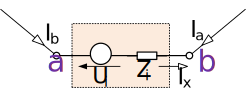
\includegraphics[width=0.7\linewidth]{Biolek_MMUN_thev_dvojpol.pdf}
          \caption[MMUN - Théveninův model dvojpólu]{Začlenění obecného lineárního dvojpólu, 
                   popsaného Théveninovým modelem do obvodu \cite[s.~78]{Biolek}}
          \label{TEO:fig_MMUN_thev_dvojpol}
        \end{figure}
        
        Původní rovnice popisující rovnováhu proudů v uzlu \emph{a} musí být na pravé straně 
        doplněna o proud $I_x$, vytékající ven z uzlu, a v uzlu \emph{b} o proud $I_x$ se záporným 
        znaménkem, protože vtéká dovnitř uzlu \emph{b}. Navíc uzlová napětí $U_a$ a $U_b$ jsou nyní 
        vázána podmínkou
        
        \begin{equation}\label{TEO:eq_MMUN_dvojpol}
          Z_iI_x + U_b = U_i + U_a, \quad\text{neboli}\quad U_i = Z_iI_x + U_b - U_a
        \end{equation}
        Všechny tyto modifikace lze zahrnout do nové soustavy rovnic MMUN:
        
        \begin{figure}[ht!]
          \centering
          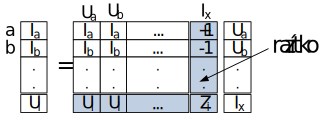
\includegraphics[width=1\linewidth]{Biolek_MMUN_razitko.pdf}
          \caption[MMUN - razítko]{ Razítko v pseudoadmitanční matici \cite[s.~79]{Biolek}}
          \label{TEO:fig_MMUN_razitko}
        \end{figure}
        
        Vektor neznámých uzlových napětí je rozšířen o další neznámou, $I_x$. Počet rovnic je 
        rovněž zvětšen o jedničku, a to o výše uvedenou podmínku mezi uzlovými napětími $U_a$ a 
        $U_b$. Přitom napětí $U_i$ je začleněno do vektoru známých budicích veličin na levé straně. 
        Modifikace rovnic 1. KZ pro uzly \emph{a} a \emph{b} je provedena zápisem $+1$ a $-1$ do 
        sloupce "$I_x$".
        
        Právě provedený zápis je návodem, jak pomocí MMUN analyzovat například obvody obsahující 
        zdroj napětí. Impedance $Z_i$ může být i nulová, pak se bude jednat o ideální zdroj napětí. 
        Při $U_i = 0$ a $I_i = 0$ lze modelovat zkrat mezi uzly a počítat proud, tekoucí tímto 
        zkratem. Toho lze využít například při analýze obvodů s proudem řízenými zdroji. 
        
        V případě, že se v obvodu nachází více prvků bez admitančního popisu, odpovídá každému z 
        nich samostatné razítko. Pseudoadmitanční matice pak nabývá na rozměrech. Metodu budeme 
        blíže konkretizovat na několika příkladech. 
  
        \subsubsection{Pasivní obvody obsahující zdroje napětí a proudu}
          Pomocí MMUN vyřešme zadání z obr. \ref{TEO:fig_MMUN02}. Je hledán proud \(I_x\) vytékající 
          ze zdroje napětí 
          %----------------------------------
          % image: TEO_fce01.tex label: \label{TEO:fig_MMUN02}
            \input{../src/TEO/img/TEO_circ02.tex}  
          %---------------------------------- 
        \subsubsection{Obvody s ideálním operačním zesilovačem ty\-pu VFA}
          Ideální OPAMP, na obr. \ref{TEO:fig_MMUN_ideal_VFA} po vložení do obvodu způsobí 
          ztotožnění uzlových napětí $U_a$ a $U_b$, a modifikaci proudových poměrů v uzlu \emph{c}.
      
          \begin{figure}[ht!]
            \centering
            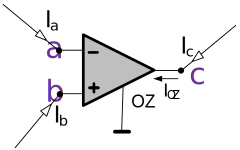
\includegraphics[width=0.6\linewidth]{MMUN_ideal_VFA.pdf}
            \caption[Ideální operační zesilovač typu VFA]{Ideální operační zesilovač typu VFA}
            \label{TEO:fig_MMUN_ideal_VFA}
          \end{figure}
          Ve spodním přídavném řádku je zapsána rovnice
          \begin{equation}\label{TEO:eq_MMUN_VFA}
              0 = 1\cdot U_a - 1\cdot U_b
          \end{equation}
          Výsledek řešení se nezmění, jestliže obě strany této rovnice vynásobíme libovolným 
          nenulovým číslem. Ve spodním řádku tedy může být namísto $[1,-1]$ například $[15,-15]$.
          \begin{figure}[ht!]
            \centering
            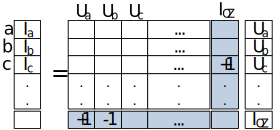
\includegraphics[width=\linewidth]{MMUN_ideal_VFA_matice.pdf}
            \caption[MMUN - pro ideální OPAMP]{MMUN - pro ideální OPAMP typu VFA}
            \label{TEO:fig_MMUN_VFA_matice}
          \end{figure}
          Je-li jeden ze vstupů OZ spojený s referenčním uzlem, neobjeví se příslušné uzlové napětí 
          v rovnicích a proto v posledním řádku bude figurovat jen jedna jednička místo uvedené 
          dvojice. 
          
          Jednička v řádku \emph{c} a sloupci $I_{OZ}$ reprezentuje připočtení proudu $I_{OZ}$ do 
          celkové bilance proudů, vytékající z uzlu \emph{c}.
        
          % --------example: Invertující zesilovač ---------------
          % \label{TEO:ex_InvOpamp01}
            % !TeX spellcheck = cs_CZ
\begin{example}\label{TEO:ex_InvOpamp01}
  Uvažujme invertující zesilovač s ideální operačním zesilovačem typu VFA s naznačenými uzly 
  tak, jak je na obr. \ref{TEO:fig_MMUN_inv_opamp}. Napište rovnice MMUN.
  
   {\centering
    \captionsetup{type=figure}
    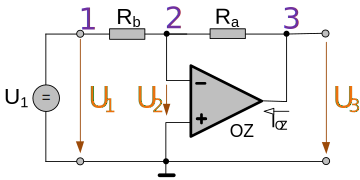
\includegraphics[width=0.7\linewidth]{MMUN_inv_OPAMP.pdf}
    \captionof{figure}{Invertující zesilovač}
    \label{TEO:fig_MMUN_inv_opamp}
    \par}
  
  Rovnice MMUN budou v maticovém zápisu vypadat takto:

    % using \usepackage{array} and command \newcolumntype{C}[1]{>{\centering}m{#1}}!
   {\centering
    \begin{tabular}{|C{0.6cm}|C{1.2cm}|C{0.6cm}|C{0.45cm}|C{0.45cm}|C{.3cm}|c|C{.33cm}|c|}
        \multicolumn{1}{c}{$U_1$}    & \multicolumn{1}{c}{$U_2$}    & \multicolumn{1}{c}{$U_3$}  & 
        \multicolumn{1}{c}{$I_1$}    & \multicolumn{1}{c}{$I_{OZ}$} & \multicolumn{1}{c}{ }      &  
        \multicolumn{1}{c}{x}        & \multicolumn{1}{c}{ }        & \multicolumn{1}{c}{b}       \\
      \cline{1-5}\cline{7-7} \cline{9-9}
      $G_b$  & $-G_b$    &  & -1  &  & \multirow{5}{*}{$\ast$} & $U_1$ & \multirow{5}{*}{=}     & \\
      \cline{1-5} \cline{7-7} \cline{9-9}
      $-G_b$ & $G_a+G_b$ & $-G_a$ &  &   & & $U_2$      &      &                                  \\
      \cline{1-5} \cline{7-7} \cline{9-9}
             & $-G_a$    & $G_a$  &  & 1 & & $U_3$      &      &                                  \\
      \cline{1-5} \cline{7-7} \cline{9-9}
         1   &           &        &  &   & & $I_1$      &      &    $U_{IN}$                      \\
      \cline{1-5} \cline{7-7} \cline{9-9}
             &     1     &        &  &   & & $I_{OZ}$   &      &                                  \\
      \cline{1-5} \cline{7-7} \cline{9-9}
    \end{tabular}
    \par}
  \vspace{1em}
  Předposlední rovnice říká, že uzlové napětí $U_1$ je rovno napětí signálového zdroje $U_{IN}$. 
  Jednička v posledním řádku reprezentuje jednoduchou rovnici $U_2 = 0$. Ačkoliv je obvod poměrně 
  jednoduchý, je pro ruční řešení neefektivní, neboť jsme získali soustavu o 5 rovnic a 5 neznámých.
\end{example}  
          %-------------------------------------------------------

          % --------example: Neinvertující zesilovač -------------
          % \label{TEO:ex_NeinvOpamp01}
            % !TeX spellcheck = cs_CZ
\begin{example}\label{TEO:ex_NeinvOpamp01} 
  Uvažujme neinvertující zesilovač s ideální operačním zesilovačem typu VFA s naznačenými uzly tak, 
  jak je na obr. \ref{TEO:fig_MMUN_neinv_opamp}. Napište rovnice MMUN.

   {\centering
    \captionsetup{type=figure}
    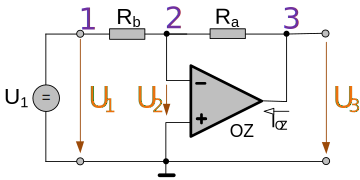
\includegraphics[width=0.7\linewidth]{MMUN_inv_OPAMP.pdf}
    \captionof{figure}{Neinvertující zesilovač}
    \label{TEO:fig_MMUN_neinv_opamp}
    \par}
   % using \usepackage{array} and command \newcolumntype{C}[1]{>{\centering}m{#1}}!
  {\centering
   \begin{tabular}{|C{0.45cm}|C{1.2cm}|C{0.6cm}|C{0.45cm}|C{0.45cm}|C{0.2cm}|c|C{.3cm}|c|}
      \multicolumn{1}{c}{$U_1$} & \multicolumn{1}{c}{$U_2$}   & \multicolumn{1}{c}{$U_3$} & 
      \multicolumn{1}{c}{$I_1$} & \multicolumn{1}{c}{$I_{OZ}$}& \multicolumn{1}{c}{ }     & 
      \multicolumn{1}{c}{x}     & \multicolumn{1}{c}{ }       & \multicolumn{1}{c}{b}     \\ 
      \cline{1-5} \cline{7-7} \cline{9-9}
           &   &   &  -1  &  & \multirow{5}{*}{$\ast$} & $U_1$ & \multirow{5}{*}{=}  &   \\
      \cline{1-5} \cline{7-7} \cline{9-9}
           & $G_a+G_b$ & $-G_a$ &      &   & & $U_2$     &   &                           \\
      \cline{1-5} \cline{7-7} \cline{9-9}
           & $-G_a$    & $G_a$ &       & 1 & & $U_3$     &   &                           \\
      \cline{1-5} \cline{7-7} \cline{9-9}
         1 &           &       &       &   & & $I_1$     &   & $U_{IN}$                  \\
      \cline{1-5} \cline{7-7} \cline{9-9}
           &     1     &       &       &   & & $I_{OZ}$  &   & $U_{IN}$                  \\
      \cline{1-5} \cline{7-7} \cline{9-9}
   \end{tabular}
   \par}
   \vspace{1em}
\end{example}  
          %-------------------------------------------------------
          \newpage
          % --------example: Diferenciální zesilovač -------------
          % \label{TEO:ex_DifOpamp01}
            % !TeX spellcheck = cs_CZ
\begin{example}\label{TEO:ex_DifOpamp01} 
  Uvažujme diferenciální zesilovač s ideální operačním zesilovačem typu VFA s naznačenými 
  uzly tak, jak je na obr. \ref{TEO:fig_MMUN_diff_opamp}. Napište rovnice MMUN.

   {\centering
    \captionsetup{type=figure}
    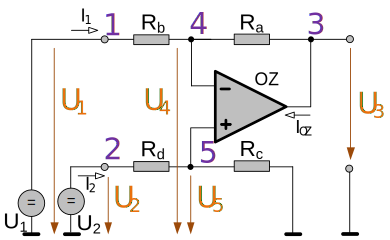
\includegraphics[width=0.7\linewidth]{MMUN_diff_OPAMP.pdf}
    \captionof{figure}{ Diferenciální zesilovač}
    \label{TEO:fig_MMUN_diff_opamp}
    \par}
%  \newpage
%  \begin{widetext}
    % using \usepackage{array} and command \newcolumntype{C}[1]{>{\centering}m{#1}}!
    {\centering
    \begin{tabular}{|C{0.6cm}|C{0.6cm}|C{0.6cm}|C{1.2cm}|C{0.6cm}|C{0.45cm}|C{0.45cm}|C{0.45cm}|}
        \multicolumn{1}{c}{$U_1$}  & \multicolumn{1}{c}{$U_2$}   & \multicolumn{1}{c}{$U_3$}  & 
        \multicolumn{1}{c}{$U_4$}  & \multicolumn{1}{c}{$U_5$}   & \multicolumn{1}{c}{$I_1$}  & 
        \multicolumn{1}{c}{$I_2$}  & \multicolumn{1}{c}{$I_{OZ}$}                      \\
        \hline
        $G_b$  &        &        & $-G_b$    &         & \(-1\) &        &             \\
        \hline
               & $G_d$  &        &           & $-G_d$  &        & \(-1\) &             \\
        \hline
               &        &  $G_a$ & $-G_a$    &         &        &        &             \\
        \hline 
        $-G_b$ &        & $-G_a$ & $G_a+G_b$ &         &        &        &             \\
        \hline
               & $-G_d$ &        & $G_c+G_d$ &         &        &        &             \\
        \hline
               &        &        &  \(-1\)   &  \(1\)  &        &        &             \\
        \hline
         1     &        &        &           &         &        &        &             \\
        \hline   
               & \(1\)  &        &           &         &        &        &             \\
        \hline    
    \end{tabular}
    \par}
%    \vspace*{0.5cm}
%  \end{widetext}
\end{example}  
          %-------------------------------------------------------

  \section{Analýza pomocí numerického simulátoru}
    \subsection{Analýza „DC“ neboli stejnosměrná analýza}
    \subsection{Rozšiřující typy analýz}
      \subsubsection{Citlivostní analýza („Sensitivity“)}
        Je počítána \emph{stejnosměrná citlivost} jedné nebo více veličin, vyjádřené vzorcem nebo 
        vzorci, na jednu nebo více vstupních proměnných.

          % --example: Citlivostní analýza napěťový děliče -------
          % \label{TEO:ex_CitDiveder01}
            % !TeX spellcheck = cs_CZ
\begin{example}\label{TEO:ex_CitDiveder01}
  V elektronických soustavách se největších přesností dosahuje u rezistorů, kde je standardně 
  zaručována chyba menší než 1\%, u přesných 0.1\% a u velmi přesných 0.01\%.

   {\centering
    \captionsetup{type=figure}
    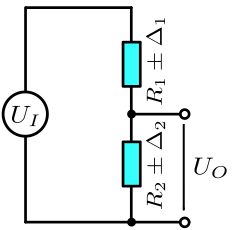
\includegraphics[width=0.4\linewidth]{voltage_divider.pdf}
    \captionof{figure}{ }
    \label{TEO:fig_voltage_divider}
    \par}

  Bude nás zajímat jaký vliv má tolerance rezistorů na výsledný poměr výstupního ku vstupnímu 
  napětí a také, zda-li při různě zvoleném poměru těchto rezistorů se bude měnit velikost chyby, 
  ačkoliv budou mít stejnou přesnost. Intuitivně předpokládáme, že  nejnepříznivější situace  
  nastane, když hodnoty použitých rezistorů padnou na opačné strany tolerančních pásem, jenž 
  reprezentuje $\Delta_1$ a $\Delta_2$ tj. $R_2 - \Delta_2R_2$ a $R_1 + \Delta_1R_1$ nebo $R_2 + 
  \Delta_2R_2$ a $R_1 - \Delta_1R_1$. V obou případech bude chyba stejná, proto si vybereme 
  například první případ a zapíšeme (rov. \ref{TEO:eq_divider_1}).
  \begin{equation}\label{TEO:eq_divider_1}
    \frac{U_o}{U_i} = \frac{R_2-\Delta_2 R_2}{R_1+\Delta_1 R_1+R_2-\Delta_2 R_2}
  \end{equation}
  a po úpravě
  \begin{equation*}
     \frac{U_o}{U_i} = \frac{(1-\Delta_2) R_2}{(1+\Delta_1) R_1+(1-\Delta_2) R_2}
  \end{equation*}
  Polynom ve jmenovateli rozvineme do následující podoby
  \begin{align*}
     [(1+\Delta_1) &+ (1-\Delta_2)](R_1+R_2)                \\
                   &= (1+\Delta_1)R_1 + (1-\Delta_2)R_2     \\
                   &+ (1+\Delta_1)R_2 + (1-\Delta_2)R_1     \\
   (1+\Delta_1)R_1 &+ (1-\Delta_2)R_2                       \\
                   &= [(1+\Delta_1)+(1-\Delta_2)](R_1+R_2)  \\
                   &- (1+\Delta_1)R_2 - (1-\Delta_2)R_1 
  \end{align*}
  a získáme %Further simplification of the denominator yields
  {\footnotesize
  \begin{equation*}
      \dfrac{U_o}{U_i}\ =
        \dfrac{(1-\Delta_2) R_2}{[(1+\Delta_1) + (1-\Delta_2)](R_1+R_2) - 
        [(1+\Delta_1) R_2\ +\ (1-\Delta_2) R_1] }
  \end{equation*}
  } %
  Nyní vydělíme jmenovatel i čitatel $(R_1 + R_2)$ a dostaneme 
  % Next divide both numerator and denominator by R1 + R2
  \begin{equation*}\label{TEO:eq_divider_2}
    \frac{U_o}{U_i}\ =\dfrac{\dfrac{(1-\Delta_2) R_2}{R_1+R2}}{[(1+\Delta_1)+(1-\Delta_2)] - 
    \dfrac{[(1+\Delta_1) R_2\ +\ (1-\Delta_2) R_1]}{R_1+R_2} }
  \end{equation*}
  Standardně rezistory volíme se stejnou tolerancí, tedy $\Delta_1 = \Delta_2 = \Delta$ a získáme 
  výslednou rovnici pro poměr $\frac{U_o}{U_i}$ 
  % Based on the assumption that both $\Delta1 = \Delta2 = \Delta$ then it should be possible to  
  % further simplify the expression for Vo/Vi:
  \begin{equation}
     \dfrac{U_o}{U_i} = \dfrac{\dfrac{(1-\Delta) R_2}{R_1+R_2}}{[(1+\Delta)+(1-\Delta)] - 
     \dfrac{[(1+\Delta)R_2 + (1-\Delta) R_1]}{R_1+R_2} }
  \end{equation}

  Řekněme například, že pro návrh děliče máme k dispozici rezistory s tolerancí 1\% a vstupní 
  napětí je 1 V. Obvod, ve kterém je dělič použit, umožňuje volit různé poměry, ale jejich součet 
  je konstantní. Na otázku jaký poměr zvolit, abychom při dané toleranci rezistorů dostali 
  výstupní napětí s největší přesností odpovídá následující tabulka.
  \vspace{1em}
  
  {\centering
   \setlength{\tabcolsep}{5pt}
   \begin{tabular}{|c|c|c|c|}
      \hline
        $R_1$                 & $1 k\Omega$  & $10 k\Omega$     & $19 k\Omega$   \\
      \hline
        $R_2$                 & $19 k\Omega$ & $10 k\Omega$     & $1 k\Omega$    \\
      \hline
        $U_{out}$             & 0,950        & 0,500            & 0,050          \\
      \hline
        $U_{out}^*$           & 0,949        & 0,495            & 0,049          \\
      \hline
        $\varepsilon_r [\%]$  & 0,101        & 1,000            & 1,883          \\
      \hline
   \end{tabular}
  \par}
  \vspace{1em}

  % Let's compare this answer to the formula I gave in a previous post using differentials. The  
  % relevant differential is
  % \begin{equation}\label{TEO:eq_divider_8}
  %   dV_0 = ( \frac{V}{R_1+R_2} - \alpha ) dR_1 - \alpha dR_2 + \frac{R_1}{R_1+R_2} dV
  % \end{equation}
  % where
  % \begin{equation}\label{TEO:eq_divider_9}
  %   \alpha = \frac{R_1 V}{(R_1+R_2)^2}
  % \end{equation}
\end{example}  
    
          %-------------------------------------------------------
} % \tikzset

%---------------------------------------------------------------------------------------------------
\printbibliography[title={Seznam literatury}, heading=subbibliography]
\addcontentsline{toc}{section}{Seznam literatury}
%========== Kapitola: Přechodné děje ==============================================================
  \input{../src/TEO/chap/teo1ch05.tex}
%========== Kapitola: Obvody v harmonickém ustáleném stavu ========================================
  \input{../src/TEO/chap/teo1ch07.tex}
%========== Kapitola: Obvody s rozprostřenými parametry ===========================================
  % !TeX spellcheck = cs_CZ
%file: teo1ch03.tex
%===========Kapitola: Obvody s rozprostřenými parametry====================================
\setchaptertoc
\chapter{Obvody s rozprostřenými parametry}\label{teo:IchapIX}

%~~~~~~~~~~~~~~~~~~~~~~~~~~~~~~~~~~~~~~~~~~~~~~~~~~~~~~~~~~~~~~~~~~~~~~~~~~~~~~~~~~~~~~~~~~~~~~~~~~  
%=============== Seznam literatury ================================================================
  \printbibliography[title={Seznam literatury}, heading=bibliography]
}  % DEBUG was off
%--------------------------------------------------------------------------------------------------
%                                       /$$$$$$$$  /$$$$$$ 
%                                       | $$_____/ /$$__  $$
%                                       | $$      | $$  \__/
%                                       | $$$$$   |  $$$$$$ 
%                                       | $$__/    \____  $$
%                                       | $$       /$$  \ $$
%                                       | $$$$$$$$|  $$$$$$/
%                                       |________/ \______/                     
%--------------------------------------------------------------------------------------------------
\ifthenelse{ \equal{\DebugMode}{true} }{ % Debug mode ON
  % !TeX program = lualatex
% !TeX root = luaking.tex
% !TeX encoding = UTF-8
% !TeX spellcheck = cs_CZ
%=================== Kapitola: Bipolární tranzistory ==============================================
\setchaptertoc
\chapter{Bipolární tranzistory}\label{es:IchapV}
  \section{Všeobecné poznatky}\label{es:IchapVsecI}
    Tranzistor je polovodičový prvek určeny na zesilovaní nebo generovaní elektrických signálu,
    jedná se tedy o \emph{aktivní} součástku.

    Podle činnosti rozdělujeme tranzistory: 
    \begin{itemize}[noitemsep]
      \item s injekcí, které využívají majoritní i minoritní nosiče (bipolární),
      \item řízené polem, které využívají pouze majoritní nosiče náboje (unipolární).
    \end{itemize}
     
    Bipolámí tranzistory představují aktivní polovodičové prvky. Jsou tvořeny dvěma přechody PN,
    tzn. třemi vrstvami z rozdílně dotovaného polovodičového materiálu. Podle pořadí vrstev
    rozlišujeme dvě skupiny bipolárních tranzistorů, a to tranzistory \textsc{NPN} a tranzistory
    \textsc{PNP}. Obě uspořádání tranzistorů jsou znázorněna na obr. \ref{teo:fig053}, kde je
    zobrazeno jak pořadí vrstev, tak příslušná schematická značka.

    \begin{figure}[ht!]
      \centering  
      \subcaptionbox{\textsc{PNP}\label{teo:fig053a}}{\luafigure[0.3]{teo_fig053a.pdf}} \hspace{1em}
      \subcaptionbox{\textsc{NPN}\label{teo:fig053b}}{\luafigure[0.3]{teo_fig053b.pdf}} \\
      \subcaptionbox{\label{teo:fig053c}}{\luafigure[0.3]{teo_fig053c.pdf}}             \hspace{1em}
      \subcaptionbox{\label{teo:fig053d}}{\luafigure[0.3]{teo_fig053d.pdf}}                   
      \caption{Pořadí vrstev polovodiče a schematická značka bipolárních NPN a PNP 
      tranzistorů (\cite[s.~112]{Frohn2006})}
      \label{teo:fig053}
    \end{figure}
    
    Označení \uv{tranzistor} je uměle vytvořené slovo z anglických slov \textbf{tran}sfer = přenášet
    a re\textbf{zistor} = odpor. Označení \uv{bipolámí} (bi = dva) má poukázat na skutečnost, že je
    hlavní proud určen dvěma rozdílnými druhy nositelů náboje. Ve všeobecném povědomí se však pro
    bipolární tranzistor ustálil zjednodušený pojem tranzistor. Na rozdíl od bipolárních tranzistorů
    teče u unipolárních tranzistorů (unum = jeden) hlavní proud pouze jedinou oblastí a z toho
    vyplývá, že je určen pouze jediným typem nositele náboje podle toho, jakým způsobem byl dotován
    polovodičový materiál. Unipolární tranzistory často označujeme jako tranzistory řízené
    elektrickým polem. Jejich princip bude uveden v kapitole \ref{es:IchapVI}.
    
    Pro uživatele má velký význam znalost vlastností a chování jednotlivých typů tranzistorů. Proto
    výrobci ke každému typu tranzistoru vydávají katalogové listy, které obsahují charakteristické
    hodnoty, charakteristiky a mezní hodnoty (obdobně jako u diod).
    
    Protože tranzistor představuje dvojbran, jenž má dvě vstupní a dvě výstupní elektrody, je počet
    charakteristických hodnot a charakteristik podstatně větší než u polovodičových diod. Některé
    důležité parametry a charakteristiky budou blíže objasněny v následujících odstavcích.
    
    Bipolární tranzistory využívají jako výchozího materiálu nejčastěji křemíku, pro vysoké kmitočty
    se používají tranzistory ze sloučenin typu \(A^{III}B^{V}\).
    
    Tranzistory můžeme rozdělovat podle mnoha hledisek. Z hlediska konstrukce je zásadní rozdělení
    na tranzistory pro malé signály (nízkého výkonu) a výkonové tranzistory. Takovéto rozdělení
    podle konstrukce je uvedeno na obr. \ref{teo:fig073}.
    
    Tranzistory nízkého výkonu se převážně používají pro zesilování malých střídavých signálů.
    Tranzistory mají v tomto případě pevně nastavený klidový pracovní bod a přiváděné signálové
    napětí je malé, tzn. že nesmějí být příliš vybuzeny. Další oblastí použití tranzistorů nízkého
    výkonu jsou elektronické spínače, které jsou buzeny v celém možném rozsahu charakteristik.
    
    Výkonové tranzistory jsou dimenzovány na velké proudy a velká napětí. Mají proto relativně větší
    pouzdra, díky nimž je možné rychleji odvádět větší množství vznikajícího tepla z krystalu
    polovodiče. Výkonové tranzistory nalézají uplatnění v zesilovačích velkých signálů, tj.
    výkonových a koncových stupních nebo zastávají funkci elektronických spínačů.

    \begin{mdframed}[style=mdnote]
      \small
      Krátce po skončení války v roce 1945, Bellovy laboratoře vytvořily skupinu pro výzkum fyziky
      pevných látek, pod vedením \textsc{Shockleyho}. Jejich cílem bylo najít alternativu ke křehkým
      elektronkovým zesilovačům. Jejich první pokusy byly založeny na Shockleyově myšlence, že
      vnější elektrické pole na polovodiči ovlivní jeho vodivost. Jejich experimenty však záhadně
      selhávaly.

      Skupina začala studovat atomové struktury, které se na povrchu a uvnitř látek liší. Hledané
      výsledky se začaly dostavovat v okamžiku, když začali obklopovat body dotyku mezi polovodičem
      a přívodními vodiči elektrolytem. \textsc{Hilbert Moore} postavil okruh, který jim dovolil
      snadno měnit frekvenci vstupního signálu a navrhl, aby používali glykol boritan, viskózní
      chemikálii, která se nevypařovala. Nakonec získali důkaz schopnosti zesílení signálu, když
      fyzik \textsc{Gerald Pearson}, podle návrhu Shockleyho, uvedl napětí na kapičku glykol
      boritanu umístěnou přes \textsc{P-N} přechod. V prosinci 1947 Bardeen a Brattain – pracovali
      bez Shockleyho – uspěli ve stvoření hrotového tranzistoru, který zesiloval signál.

      Další měsíc začali patentoví zástupci Bellových laboratoří pracovat na patentových
      přihláškách. Brzo objevili, že Shockleyho vliv elektrického pole na polovodič byl předpovídán
      a patentován v roce 1930 \textsc{Juliem Lilienfeldem}, který si svůj \textsc{MESFET}
      patentoval v Kanadě již v 22. října 1925. Přesto byly podány celkem čtyři žádosti o patent. Na
      žádné z těchto přihlášek se však nevyskytovalo Shockleyovo jméno. To Shockleyho rozzlobilo,
      protože práce byla založena na jeho nápadu s účinkem elektrického pole. 
      
      Ve stejnou dobu tiše pokračoval ve vlastní práci na stavbě různých druhů tranzistoru
      založených na spojení místo bodového dotyku. Předpokládal, že tento typ tranzistoru bude více
      komerčně úspěšný. Shockley pracoval na \emph{teorii elektronů a děr v polovodičích}, která
      byla nakonec vydána jako 558 stránková monografie v roce 1950. V té Shockley vypracoval
      rozhodující myšlenky týkající se pohybu elektronů a děr a diferenciální rovnici, kterou se
      řídí tok elektronů v pevných krystalech.

      Shockleyho tato práce vedla k myšlence \emph{sendvičového tranzistoru} a ke vzniku klasického
      tranzistoru. Jeho objev byl oznámen 4. června 1951 a Shockley obdržel 25. září 1951 za jeho
      objev patent. Pro výrobu tohoto tranzistoru byla vyvinuta difúzní metoda a tento tranzistor
      brzy zastínil tranzistor s bodovými kontakty. Shockley pokračoval jako vedoucí skupiny v
      Bellových laboratořích ještě dva roky.

      {\centering
        \captionsetup{type=figure}
        \luafigure[1]{teo_fig071.png}
        \captionof{figure}{\textsc{John Bardeen}, \textsc{William Shockley} a \textsc{Walter Brattain} 
          v Bell Labs, 1948. (\cite[s.~6]{KolkaBiolek2011})
        \label{teo:fig071}}
      \par}

      V roce 1951 byl zvolen členem National Academy of Sciences (NAS). Za svůj objev tranzistoru
      získal mnoho cen. Bellovy laboratoře však představovaly všechny tři vynálezce (Shockleyho,
      Bardeena a Brattaina) jako tým. To vedlo k rozkolu a Shockley později blokoval práci Bardeena
      a Brattaina na klasickém tranzistoru.

      Shockley nakonec začal řídit svoji vlastní společnost, v níž se pokoušel vytvořit nové a
      technicky obtížné zařízení (původně nazvané čtyřvrstvá dioda a nyní známé jako tyristor).
      Projekt se ale rozvíjel velmi pomalu. 

      V roce 1956 Shockley získal, spolu s Bardeenem a Brattainem, Nobelovu cenu za fyziku. Ve své
      Nobelovské přednášce plně ocenil Brattaina a Bardeena jako vynálezce tranzistoru s bodovými
      kontakty.
    \end{mdframed}
    
    Pro lepší orientaci ve velkém množství vyráběných typů tranzistorů bylo zavedeno označovací
    schéma. Evropští výrobci používají hlavně značení \uv{Pro-Electron\footnote{Pro Electron nebo
    EECA je evropský typový a registrační systém pro aktivní komponenty (jako jsou polovodiče,
    displeje z tekutých krystalů, senzorová zařízení, elektronky a katodové trubice). Společnost Pro
    Electron byla založena v roce 1966 v belgickém Bruselu. V roce 1983 byla sloučena s Evropskou
    asociací výrobců elektronických součástek (EECA) a od té doby působí jako agentura EECA.}},
    které využívá kombinace písmen a číslic.

    \luagraphic[1]{teo_fig079.jpg}{Pohled na čip \textsc{MJ1000} v TO3 pouzdře. Čip obsahuje dva 
      tranzistory v Darlingtonovo zapojení. První, méně výkonný tranzistor se zesílením cca 100 
      budí druhý výkonový tranzistor se zesílením cca 10. Výsledný zesilovací činitel je dán 
      přibližně vynásobením zesilovacích činitelů obou tranzistorů (cca 1000).}{teo:fig079}

    Aby mohl tranzistor řádně pracovat, musí mít potřebné napětí nejen mezi kolektorem a emitorem,
    ale také dostatečně velké napětí mezi bází a emitorem. Velkou roli přitom hraje teplotní
    stabilizace klidového pracovního bodu. Je potřebná z toho důvodu, že při stoupající teplotě
    okolí narůstají též proudy, které tranzistorem protékají. Následkem zvyšování teploty se krystal
    ohřívá a roste tak jeho vodivost, čímž se příslušné proudy zvětšují. Tímto způsobem stoupá
    ztrátový výkon, tranzistor se proto více ohřívá atd. Na konci tohoto koloběhu je tepelná
    destrukce tranzistoru, který se tak stává nepoužitelným.

    \begin{figure*}
      \centering
      \luafigure[1]{teo_fig073.png}
      \caption{Druhy bipolárních tranzistorů podle konstrukce. (\cite[s.~115]{Frohn2006})}
      \label{teo:fig073}
    \end{figure*}

    Tranzistory mohou pracovat ve třech různých základních zapojeních - se společným emitorem
    (\textsc{SE}), se společným kolektorem (\textsc{SC}) a se společnou bází (\textsc{SB}). Zapojení
    je pojmenováno podle toho, která z elektrod je společná vstupu a výstupu zesilovacího stupně pro
    zesilování střídavých napětí, tj. která představuje společný pól signálového napětí na vstupu a
    na výstupu daného stupně. Každé z těchto základních zapojení má své přednosti a nedostatky.
    Nejčastěji se používá zapojení \textsc{SE}. Zapojení \textsc{SC} se používá jako měnič impedance
    (velká vstupní a malá výstupní impedance). Zapojení \textsc{SB} má svůj význam hlavně ve
    vysokofrekvenční technice, jinak představuje také měnič impedance, avšak s přesně opačným
    účinkem než předchozí zapojení (malá vstupní a velká výstupní impedance).

    Při praktickém využití musejí být tranzistory, a to ať se jedná o jakékoliv zapojení, doplněny
    dalšími součástkami. Zapojení těchto součástek (rezistorů a kondenzátorů) závisí na tom, jakou
    úlohu má zapojení s tranzistorem plnit. Musíme rozlišit, zda má tranzistor pracovat ve
    stejnosměrném zesilovači, v zesilovači střídavých napětí, ve výkonovém zesilovači nebo zda má
    mít funkci spínače.

    Stejnosměrné zesilovače se používají všude tam, kde je zapotřebí zesilovat stejnosměrná napětí a
    změny napětí od velmi malých až k vysokým frekvencím. Typickým představitelem je např. zesilovač
    Y osciloskopu. Aby stejnosměrné zesilovače mohly řádně plnit svou funkci, nesmějí obsahovat
    žádné součástky, které by ovlivňovaly jejich zesílení na různých frekvencích a neumožňovaly
    galvanickou vazbu (např. kondenzátory).

    Střídavé zesilovače mohou naproti tomu zesilovat střídavá napětí o frekvenci několika \si{\Hz}
    až do několika \si{\GHz} (podle typu tranzistoru a dimenzování zapojení), avšak nemusejí
    zesilovat stejnosměrná napětí. Důležitými prvky v těchto zesilovačích jsou kondenzátory.

    Výkonové zesilovače mají spotřebiči odevzdat pokud možno co největší signálový výkon. Spotřebič
    může být představován např. reproduktorem (nízkofrekvenční výkonový zesilovač), vysílací anténou
    (vysokofrekvenční výkonový zesilovač) nebo motorem (aplikace výkonového zesilovače v regulační
    technice). Na spínače jsou kladeny zcela jiné požadavky než na stejnosměrné nebo střídavé
    zesilovače. Spínače mají co nejrychleji přecházet ze stavu \uv{zapnuto} do stavu \uv{vypnuto} a
    naopak. V tomto případě hrají velkou roli parazitní kapacity tranzistorů.


  \section{Základní princip}\label{es:IchapVsecII}
    \subsection{Princip funkce NPN a PNP tranzistorů}\label{es:IchapVsecIIssecI}
      První tranzistory byly vyráběny legováním. Tato technologie byla převzata z výroby diod. Aby
      byly vyrobeny dva přechody, byly na obě strany dotovaného základního materiálu umístěny
      pilulky cizích prvků - donorů nebo akceptorů {obr. \ref{teo:fig072}. Při výrobním procesu pak
      cizí atomy z obou stran difundovaly do výchozího materiálu. Střední vrstva byla přitom velmi
      tenká a měla výrazně menší počet volných nositelů náboje než obě vnější vrstvy. Podle
      použitých výchozích materiálů a cizích prvků vznikl tranzistor NPN nebo PNP.

      \luagraphic[0.8]{teo_fig072.png}{Výroba tranzistoru NPN legováním.
        (\cite[s.~115]{Frohn2006})}{teo:fig072}
      
      Aby tranzistor fungoval, musí být mezi bázi a emitor připojen zdroj napětí tak, aby byl spodní
      přechod PN polarizován v propustném směru. Tranzistor NPN má proto bázi kladnější než emitor,
      tranzistor PNP má bázi zápornější než emitor. Napětí mezi bází a emitorem křemíkových
      tranzistorů má velikost \(U_{BE} \approx \SI{0.7}{\V}\), tj. stejné, jako je difuzní napětí
      křemíkových diod. Na obr. \ref{teo:fig074} a \ref{teo:fig075} zakreslené proudy vyznačují směr
      toku elektronů.

      \luagraphic[1]{teo_fig074.png}{Znázornění tranzistoru NPN. \(\longrightarrow\) udáva směr 
        toku elektronů). (\cite[s.~116]{Frohn2006})}{teo:fig074}
      
      Horní přechod PN pracuje v závěrném směru. Zdroje napětí jsou z tohoto důvodu zapojeny tak,
      aby byl kolektor u NPN tranzistoru kladnější než emitor, u PNP tranzistoru naopak zápornější
      než emitor.

      Vlivem připojených napětí bude spodní přechod PN zapojen v propustném směru a horní přechod PN
      v závěrném směru. Ve střední a horní oblasti se vytvoří závěrná vrstva. Ta se rozprostírá
      téměř po celé šířce střední oblasti, která je velmi tenká a obsahuje pouze malý počet nositelů
      náboje.        

      \luagraphic[1]{teo_fig075.png}{Znázornění tranzistoru PNP.  \(\longrightarrow\) udáva směr 
        toku elektronů). (\cite[s.~116]{Frohn2006})}{teo:fig075}
      
      Protože je spodní přechod PN zapojen v propustném směru, zaplavují nositelé náboje z emitoru
      závěrnou vrstvu ve střední oblasti. Tím se tato závěrná vrstva zmenší a její odpor klesne. Tím
      mohou nositelé náboje z emitoru projít zmenšenou závěrnou vrstvou do kolektorové oblasti a
      odtud odtéct k baterii (ke zdroji).

      Jelikož nositelé náboje pocházejí ze spodní oblasti, nazývá se tato oblast emitor. Střední
      oblast představuje výchozí bod pro oba přechody PN a nazývá se proto bází. Horní oblast
      shromažďuje všechny nositele náboje, které neodtekly bází a nese označení kolektor.

      \luagraphic[1]{teo_fig076.png}{Provozní napětí a proudy tranzistoru NPN. 
        (\cite[s.~117]{Frohn2006})}{teo:fig076}
      
      Proud \(l_B\), který odtéká vývodem báze, je podstatně menší než kolektorový proud \(l_C\),
      jenž protéká zmenšenou závěrnou vrstvou. Např. při napětí \(U_{BE} \approx \SI{0.7}{\V}\)
      protéká bází proud \(I_B = \SI{1}{\mA}\) a kolektorem proud \(I_C \approx \SI{100}{\mA}\).
      Jestliže nyní nepatrné zvětšíme \(U_{BE}\), vzroste proud báze např. na \(I_B = \SI{2}{\mA}\),
      čímž k závěrné vrstvě doputuje více nositelů náboje z emitoru. Tím se závěrná vrstva ještě
      více zmenší a kolektorový proud vzroste např. na \(I_C \approx \SI{200}{\mA}\). Naopak při
      zmenšení napětí \(U_{BE}\) a tím též proudu \(l_B\) se odpor závěrné vrstvy zvětší a
      kolektorový proud \(I_C\) klesne. Zjišťujeme, že proud báze \(l_B\) a proud kolektoru \(l_C\)
      tranzistoru se v širokém rozmezí mění proporcionálně. U tranzistoru je tak možné malým proudem
      báze \(l_B\), jenž představuje vstupní proud, řídit podstatně větší kolektorový proud \(l_C\),
      který je výstupním proudem. Tato souvislost se udává formou \emph{proudového zesílení
      nakrátko} \(\beta\).

      \begin{equation*}
        \beta = \dfrac{\Delta I_C}{\Delta I_B} \qquad \text{při (\(U_{CE} = 0\))}
      \end{equation*}
        
      \luagraphic[1]{teo_fig077.png}{Provozní napětí a proudy tranzistoru PNP. 
        (\cite[s.~117]{Frohn2006})}{teo:fig077}
      
      Tranzistory NPN a PNP se navzájem principiálně odlišují pořadím vrstev. Proto se odlišují též
      polaritou napětí \(U_{BE}\) a \(U_{CE}\). Obr. \ref {teo:fig076} a \ref {teo:fig077}
      vysvětluje souvislosti, které již byly naznačeny na obr. \ref{teo:fig074} a \ref{teo:fig075},
      tentokrát jsou ale použity schematické značky obou typů tranzistorů. Údaj napětí \(U_BE\) a
      \(U_{CE}\) je tvořen tak, že poslední písmeno udává vztažnou elektrodu, zde tedy emitor E. Při
      určování směru toku proudu vycházíme z technické orientace, jež je obvyklá (proud teče obvodem
      směrem od kladného k zápornému pólu zdroje). Všechny proudy, které tečou do tranzistoru, jsou
      kladné, vytékající proudy mají záporné znaménko.

      Aby byl tranzistor schopen činnosti, musí být vždy přechod báze-emitor v propustném směru a
      přechod báze-kolektor v závěrném směru.

      Na obr. \ref{teo:fig078a} je mezi vývod kolektoru a baterii zařazen ještě kolektorový rezistor
      \(R_C\), který plní funkci pracovního odporu. Ten omezuje proudové zesílení tranzistoru a
      přeměňuje je v napěťové zesílení. Tranzistor a kolektorový rezistor v tomto případě tvoří
      napěťový dělič pro napájecí napětí \(U_{CC} = \SI{+10}{\V}\). Při \(I_C = \SI{5}{\mA}\) a
      \(R_C = \SI{1}{\kohm}\) vzniká na kolektorovém rezistoru úbytek napětí
      \begin{equation*}
        U_{RC} = \SI{5e-3}{\mA}\cdot\SI{1}{\kohm} = \SI{5}{\V}
      \end{equation*}

      \luagraphic[1]{teo_fig078a.jpg}{apěťové zesílení tranzistoru NPN. 
        (\cite[s.~117]{Frohn2006})}{teo:fig078a}

      Napětí kolektor-emitor tranzistoru, které představuje výstupní napětí, bude 
      \begin{equation*}
        U_{CE} = U_{CC} - U_{RC} = \SI{10}{\V} - \SI{5}{\V} = \SI{5}{\V}
      \end{equation*}
      Jestliže se napětí \(U_{BE}\) vlivem střídavého napětí z připojeného generátoru v daný okamžik
      zvětší např. na \(U_{BE} = \SI{0.71}{\V}\), vzroste proud báze, který způsobí zvětšení
      kolektorového proudu, který, dejme tomu, vzroste z \(I_C = \SI{5}{\mA}\) na \(I_C =
      \SI{6.5}{\mA}\). Tento zvětšený kolektorový proud vyvolá na kolektorovém rezistoru zvětšený
      úbytek napětí
      \begin{equation*}
        U_{RC} = I_C\cdot R_C = \SI{6.5}{\mA}\cdot\SI{1}{\kohm} = \SI{6.5}{\V}
      \end{equation*}
      Tím napětí \(U_{CE}\) klesne na hodnotu \(U_{CE} = \SI{3.5}{\V}\). Při záporné půlvlně napětí
      generátoru se proud báze \(I_B\) zmenší, čímž se zmenši i proud kolektoru \(l_C\) a tím i
      úbytek napětí na kolektorovém rezistoru \(U_{RC}\). Důsledkem tohoto děje je zvětšení
      \(l_{CE}\) tranzistoru. Příslušné časové průběhy na obr. \ref{teo:fig078}. Generátor,
      připojený na bázi tranzistoru, způsobí změnu proudu báze \(\Delta I_B = \SI{20}{\micro\A}\),
      která vyvolá změnu kolektorového proudu \(\Delta I_C = \SI{3}{\mA}\).

      \begin{figure}[ht!]  %\ref{teo:fig078} 
        \centering
        \subcaptionbox{\(U_{BE}(t)\)\label{teo:fig078b}}{\luafigure[0.9]{teo_fig078b.jpg}}  \\                                                       
        \subcaptionbox{\(I_{B}(t)\) \label{teo:fig078c}}{\luafigure[0.9]{teo_fig078c.jpg}}  \\                  
        \subcaptionbox{\(I_{C}(t)\) \label{teo:fig078d}}{\luafigure[0.9]{teo_fig078d.jpg}}  \\                 
        \subcaptionbox{\(U_{RC}(t)\)\label{teo:fig078e}}{\luafigure[0.9]{teo_fig078e.jpg}}  \\                  
        \subcaptionbox{\(U_{CE}(t)\)\label{teo:fig078f}}{\luafigure[0.9]{teo_fig078f.jpg}}  \\                   
        \caption{Napěťové zesílení tranzistoru zapojeného podle obr. \ref{teo:fig078a} 
          (\cite[s.~118]{Frohn2006})}
        \label{teo:fig078}
      \end{figure}

      Odtud pro uvedený případ zjistíme \emph{proudové zesílení} tranzistoru
      \begin{equation*}
        \beta = \dfrac{\Delta I_C}{\Delta I_B} = \dfrac{\num{3e-3}}{\num{20e-6}} = 150
      \end{equation*}
      \emph{Napěťové zesílení} \(A_u\) zapojení s tranzistorem je definováno podobně jako proudové
      zesílení.
      \begin{equation*}
        A_u = \dfrac{\Delta U_{out}}{\Delta U_{in}} = \dfrac{\Delta U_{CE}}{\Delta U_{BE}}
      \end{equation*}
      Napěťové zesílení závisí kromě proudového zesílení také na velikosti kolektorového rezistoru
      \(R_C\). V příkladu způsobí vstupní střídavé napětí \(\Delta U_{BE} = \SI{-0.02}{\V}\) změnu
      výstupního střídavého napětí \(U_{CE} = \SI{-3}{\V}\). V tomto případě je tedy napěťové
      zesílení
      \begin{equation*}
        A_u = \dfrac{\Delta U_{CE}}{\Delta U_{BE}} = \dfrac{\num{-3}}{\num{0.02}} = -150
      \end{equation*}
      Pomocí kolektorového rezistoru \(R_{C}\) se změnilo proudové zesílení na napěťové zesílení
      tranzistoru. Znaménko \uv{-} naznačuje, že kladné půlvlně vstupního napětí odpovídá záporná
      půlvlna výstupního napětí.

  \section{Základní zapojení tranzistoru}\label{es:IchapVsecIII}
%---------------------------------------------------------------------------------------------------
}{ % DEBUG was off
\LuaPartBckgrnd{titleBG_fractal1.png}
\LuaPartTitle{ES I}{Elektronické součástky}{ESI}
\parttoc
%========== Kapitola: Pasivni součástky ==========================================================
  % !TeX spellcheck = cs_CZ
% file: kap_optocoupler.tex
%{\tikzset{external/prefix={tikz/TEO/}}
% \tikzset{external/figure name/.add={ch12_}{}}
%=================== Kapitola: Optoelektronika =====================================================
\setchaptertoc
\chapter{Pasivní elektronické součáskty}\label{teo:IchapXII}


  \section{Teplotní závislost pasivních prvků}\label{teo:IchapXIIsecI}
    
    \begin{example}\label{teo:exam001}
      Uvažujeme žárovku \qty{100}{\watt}, \qty{230}{\volt} s wolframovým vláknem s teplotním 
      součinitelem odporu \(\alpha = \qty{4.8e-3}{\per\kelvin}\).  Problematické je určení provozní 
      teploty vlákna. Vzhledem k tomu, že wolfram taje při teplotě \qty{3387}{\degreeCelsius} a 
      vlákno svítí bílým žárem, odhadneme teplotu na \qty{2500}{\degreeCelsius}. Ze vztahu \(P = 
      U^2/R\) určíme odpor vlákna: \(R = 230^2/100 = \qty{529}{\ohm}\). Odpor při pokojové teplotě 
      bude: 
      \(R_{20}=529/(1+\num{4.8e-3}\cdot2480) = \qty{41}{\ohm}\). 
      \begin{figure}[ht!]  %\ref{teo:fig018}
        \centering
        \includegraphics[width=0.3\linewidth]{teo_fig018.jpg}
        \caption{Žárovka jednoduchým způsobem přeměňuje elektrickou energii na světlo, zahříváním 
        tenkého wolframového vodiče průchodem elektrického proudu.}
        \label{teo:fig018}
      \end{figure}
      Podle tohoto přibližného výpočtu se zmenší odpor vlákna  téměř třináctkrát a odpovídajícím 
      způsobem vzrůstá i nárazový proud při zapnutí obvodu oproti ustálenému stavu. Z tohoto 
      pohledu měly původní Edisonovy uhlíkové žárovky lepší vlastnosti, protože teplotní součinitel 
      uhlíku je záporný (\cite[s.~84]{Lanicek1998}).
    \end{example}
%} % tikzset
%---------------------------------------------------------------------------------------------------
%========== Kapitola: Bipolární transzistory =====================================================
  % !TeX program = lualatex
% !TeX root = luaking.tex
% !TeX encoding = UTF-8
% !TeX spellcheck = cs_CZ
%=================== Kapitola: Bipolární tranzistory ==============================================
\setchaptertoc
\chapter{Bipolární tranzistory}\label{es:IchapV}
  \section{Všeobecné poznatky}\label{es:IchapVsecI}
    Tranzistor je polovodičový prvek určeny na zesilovaní nebo generovaní elektrických signálu,
    jedná se tedy o \emph{aktivní} součástku.

    Podle činnosti rozdělujeme tranzistory: 
    \begin{itemize}[noitemsep]
      \item s injekcí, které využívají majoritní i minoritní nosiče (bipolární),
      \item řízené polem, které využívají pouze majoritní nosiče náboje (unipolární).
    \end{itemize}
     
    Bipolámí tranzistory představují aktivní polovodičové prvky. Jsou tvořeny dvěma přechody PN,
    tzn. třemi vrstvami z rozdílně dotovaného polovodičového materiálu. Podle pořadí vrstev
    rozlišujeme dvě skupiny bipolárních tranzistorů, a to tranzistory \textsc{NPN} a tranzistory
    \textsc{PNP}. Obě uspořádání tranzistorů jsou znázorněna na obr. \ref{teo:fig053}, kde je
    zobrazeno jak pořadí vrstev, tak příslušná schematická značka.

    \begin{figure}[ht!]
      \centering  
      \subcaptionbox{\textsc{PNP}\label{teo:fig053a}}{\luafigure[0.3]{teo_fig053a.pdf}} \hspace{1em}
      \subcaptionbox{\textsc{NPN}\label{teo:fig053b}}{\luafigure[0.3]{teo_fig053b.pdf}} \\
      \subcaptionbox{\label{teo:fig053c}}{\luafigure[0.3]{teo_fig053c.pdf}}             \hspace{1em}
      \subcaptionbox{\label{teo:fig053d}}{\luafigure[0.3]{teo_fig053d.pdf}}                   
      \caption{Pořadí vrstev polovodiče a schematická značka bipolárních NPN a PNP 
      tranzistorů (\cite[s.~112]{Frohn2006})}
      \label{teo:fig053}
    \end{figure}
    
    Označení \uv{tranzistor} je uměle vytvořené slovo z anglických slov \textbf{tran}sfer = přenášet
    a re\textbf{zistor} = odpor. Označení \uv{bipolámí} (bi = dva) má poukázat na skutečnost, že je
    hlavní proud určen dvěma rozdílnými druhy nositelů náboje. Ve všeobecném povědomí se však pro
    bipolární tranzistor ustálil zjednodušený pojem tranzistor. Na rozdíl od bipolárních tranzistorů
    teče u unipolárních tranzistorů (unum = jeden) hlavní proud pouze jedinou oblastí a z toho
    vyplývá, že je určen pouze jediným typem nositele náboje podle toho, jakým způsobem byl dotován
    polovodičový materiál. Unipolární tranzistory často označujeme jako tranzistory řízené
    elektrickým polem. Jejich princip bude uveden v kapitole \ref{es:IchapVI}.
    
    Pro uživatele má velký význam znalost vlastností a chování jednotlivých typů tranzistorů. Proto
    výrobci ke každému typu tranzistoru vydávají katalogové listy, které obsahují charakteristické
    hodnoty, charakteristiky a mezní hodnoty (obdobně jako u diod).
    
    Protože tranzistor představuje dvojbran, jenž má dvě vstupní a dvě výstupní elektrody, je počet
    charakteristických hodnot a charakteristik podstatně větší než u polovodičových diod. Některé
    důležité parametry a charakteristiky budou blíže objasněny v následujících odstavcích.
    
    Bipolární tranzistory využívají jako výchozího materiálu nejčastěji křemíku, pro vysoké kmitočty
    se používají tranzistory ze sloučenin typu \(A^{III}B^{V}\).
    
    Tranzistory můžeme rozdělovat podle mnoha hledisek. Z hlediska konstrukce je zásadní rozdělení
    na tranzistory pro malé signály (nízkého výkonu) a výkonové tranzistory. Takovéto rozdělení
    podle konstrukce je uvedeno na obr. \ref{teo:fig073}.
    
    Tranzistory nízkého výkonu se převážně používají pro zesilování malých střídavých signálů.
    Tranzistory mají v tomto případě pevně nastavený klidový pracovní bod a přiváděné signálové
    napětí je malé, tzn. že nesmějí být příliš vybuzeny. Další oblastí použití tranzistorů nízkého
    výkonu jsou elektronické spínače, které jsou buzeny v celém možném rozsahu charakteristik.
    
    Výkonové tranzistory jsou dimenzovány na velké proudy a velká napětí. Mají proto relativně větší
    pouzdra, díky nimž je možné rychleji odvádět větší množství vznikajícího tepla z krystalu
    polovodiče. Výkonové tranzistory nalézají uplatnění v zesilovačích velkých signálů, tj.
    výkonových a koncových stupních nebo zastávají funkci elektronických spínačů.

    \begin{mdframed}[style=mdnote]
      \small
      Krátce po skončení války v roce 1945, Bellovy laboratoře vytvořily skupinu pro výzkum fyziky
      pevných látek, pod vedením \textsc{Shockleyho}. Jejich cílem bylo najít alternativu ke křehkým
      elektronkovým zesilovačům. Jejich první pokusy byly založeny na Shockleyově myšlence, že
      vnější elektrické pole na polovodiči ovlivní jeho vodivost. Jejich experimenty však záhadně
      selhávaly.

      Skupina začala studovat atomové struktury, které se na povrchu a uvnitř látek liší. Hledané
      výsledky se začaly dostavovat v okamžiku, když začali obklopovat body dotyku mezi polovodičem
      a přívodními vodiči elektrolytem. \textsc{Hilbert Moore} postavil okruh, který jim dovolil
      snadno měnit frekvenci vstupního signálu a navrhl, aby používali glykol boritan, viskózní
      chemikálii, která se nevypařovala. Nakonec získali důkaz schopnosti zesílení signálu, když
      fyzik \textsc{Gerald Pearson}, podle návrhu Shockleyho, uvedl napětí na kapičku glykol
      boritanu umístěnou přes \textsc{P-N} přechod. V prosinci 1947 Bardeen a Brattain – pracovali
      bez Shockleyho – uspěli ve stvoření hrotového tranzistoru, který zesiloval signál.

      Další měsíc začali patentoví zástupci Bellových laboratoří pracovat na patentových
      přihláškách. Brzo objevili, že Shockleyho vliv elektrického pole na polovodič byl předpovídán
      a patentován v roce 1930 \textsc{Juliem Lilienfeldem}, který si svůj \textsc{MESFET}
      patentoval v Kanadě již v 22. října 1925. Přesto byly podány celkem čtyři žádosti o patent. Na
      žádné z těchto přihlášek se však nevyskytovalo Shockleyovo jméno. To Shockleyho rozzlobilo,
      protože práce byla založena na jeho nápadu s účinkem elektrického pole. 
      
      Ve stejnou dobu tiše pokračoval ve vlastní práci na stavbě různých druhů tranzistoru
      založených na spojení místo bodového dotyku. Předpokládal, že tento typ tranzistoru bude více
      komerčně úspěšný. Shockley pracoval na \emph{teorii elektronů a děr v polovodičích}, která
      byla nakonec vydána jako 558 stránková monografie v roce 1950. V té Shockley vypracoval
      rozhodující myšlenky týkající se pohybu elektronů a děr a diferenciální rovnici, kterou se
      řídí tok elektronů v pevných krystalech.

      Shockleyho tato práce vedla k myšlence \emph{sendvičového tranzistoru} a ke vzniku klasického
      tranzistoru. Jeho objev byl oznámen 4. června 1951 a Shockley obdržel 25. září 1951 za jeho
      objev patent. Pro výrobu tohoto tranzistoru byla vyvinuta difúzní metoda a tento tranzistor
      brzy zastínil tranzistor s bodovými kontakty. Shockley pokračoval jako vedoucí skupiny v
      Bellových laboratořích ještě dva roky.

      {\centering
        \captionsetup{type=figure}
        \luafigure[1]{teo_fig071.png}
        \captionof{figure}{\textsc{John Bardeen}, \textsc{William Shockley} a \textsc{Walter Brattain} 
          v Bell Labs, 1948. (\cite[s.~6]{KolkaBiolek2011})
        \label{teo:fig071}}
      \par}

      V roce 1951 byl zvolen členem National Academy of Sciences (NAS). Za svůj objev tranzistoru
      získal mnoho cen. Bellovy laboratoře však představovaly všechny tři vynálezce (Shockleyho,
      Bardeena a Brattaina) jako tým. To vedlo k rozkolu a Shockley později blokoval práci Bardeena
      a Brattaina na klasickém tranzistoru.

      Shockley nakonec začal řídit svoji vlastní společnost, v níž se pokoušel vytvořit nové a
      technicky obtížné zařízení (původně nazvané čtyřvrstvá dioda a nyní známé jako tyristor).
      Projekt se ale rozvíjel velmi pomalu. 

      V roce 1956 Shockley získal, spolu s Bardeenem a Brattainem, Nobelovu cenu za fyziku. Ve své
      Nobelovské přednášce plně ocenil Brattaina a Bardeena jako vynálezce tranzistoru s bodovými
      kontakty.
    \end{mdframed}
    
    Pro lepší orientaci ve velkém množství vyráběných typů tranzistorů bylo zavedeno označovací
    schéma. Evropští výrobci používají hlavně značení \uv{Pro-Electron\footnote{Pro Electron nebo
    EECA je evropský typový a registrační systém pro aktivní komponenty (jako jsou polovodiče,
    displeje z tekutých krystalů, senzorová zařízení, elektronky a katodové trubice). Společnost Pro
    Electron byla založena v roce 1966 v belgickém Bruselu. V roce 1983 byla sloučena s Evropskou
    asociací výrobců elektronických součástek (EECA) a od té doby působí jako agentura EECA.}},
    které využívá kombinace písmen a číslic.

    \luagraphic[1]{teo_fig079.jpg}{Pohled na čip \textsc{MJ1000} v TO3 pouzdře. Čip obsahuje dva 
      tranzistory v Darlingtonovo zapojení. První, méně výkonný tranzistor se zesílením cca 100 
      budí druhý výkonový tranzistor se zesílením cca 10. Výsledný zesilovací činitel je dán 
      přibližně vynásobením zesilovacích činitelů obou tranzistorů (cca 1000).}{teo:fig079}

    Aby mohl tranzistor řádně pracovat, musí mít potřebné napětí nejen mezi kolektorem a emitorem,
    ale také dostatečně velké napětí mezi bází a emitorem. Velkou roli přitom hraje teplotní
    stabilizace klidového pracovního bodu. Je potřebná z toho důvodu, že při stoupající teplotě
    okolí narůstají též proudy, které tranzistorem protékají. Následkem zvyšování teploty se krystal
    ohřívá a roste tak jeho vodivost, čímž se příslušné proudy zvětšují. Tímto způsobem stoupá
    ztrátový výkon, tranzistor se proto více ohřívá atd. Na konci tohoto koloběhu je tepelná
    destrukce tranzistoru, který se tak stává nepoužitelným.

    \begin{figure*}
      \centering
      \luafigure[1]{teo_fig073.png}
      \caption{Druhy bipolárních tranzistorů podle konstrukce. (\cite[s.~115]{Frohn2006})}
      \label{teo:fig073}
    \end{figure*}

    Tranzistory mohou pracovat ve třech různých základních zapojeních - se společným emitorem
    (\textsc{SE}), se společným kolektorem (\textsc{SC}) a se společnou bází (\textsc{SB}). Zapojení
    je pojmenováno podle toho, která z elektrod je společná vstupu a výstupu zesilovacího stupně pro
    zesilování střídavých napětí, tj. která představuje společný pól signálového napětí na vstupu a
    na výstupu daného stupně. Každé z těchto základních zapojení má své přednosti a nedostatky.
    Nejčastěji se používá zapojení \textsc{SE}. Zapojení \textsc{SC} se používá jako měnič impedance
    (velká vstupní a malá výstupní impedance). Zapojení \textsc{SB} má svůj význam hlavně ve
    vysokofrekvenční technice, jinak představuje také měnič impedance, avšak s přesně opačným
    účinkem než předchozí zapojení (malá vstupní a velká výstupní impedance).

    Při praktickém využití musejí být tranzistory, a to ať se jedná o jakékoliv zapojení, doplněny
    dalšími součástkami. Zapojení těchto součástek (rezistorů a kondenzátorů) závisí na tom, jakou
    úlohu má zapojení s tranzistorem plnit. Musíme rozlišit, zda má tranzistor pracovat ve
    stejnosměrném zesilovači, v zesilovači střídavých napětí, ve výkonovém zesilovači nebo zda má
    mít funkci spínače.

    Stejnosměrné zesilovače se používají všude tam, kde je zapotřebí zesilovat stejnosměrná napětí a
    změny napětí od velmi malých až k vysokým frekvencím. Typickým představitelem je např. zesilovač
    Y osciloskopu. Aby stejnosměrné zesilovače mohly řádně plnit svou funkci, nesmějí obsahovat
    žádné součástky, které by ovlivňovaly jejich zesílení na různých frekvencích a neumožňovaly
    galvanickou vazbu (např. kondenzátory).

    Střídavé zesilovače mohou naproti tomu zesilovat střídavá napětí o frekvenci několika \si{\Hz}
    až do několika \si{\GHz} (podle typu tranzistoru a dimenzování zapojení), avšak nemusejí
    zesilovat stejnosměrná napětí. Důležitými prvky v těchto zesilovačích jsou kondenzátory.

    Výkonové zesilovače mají spotřebiči odevzdat pokud možno co největší signálový výkon. Spotřebič
    může být představován např. reproduktorem (nízkofrekvenční výkonový zesilovač), vysílací anténou
    (vysokofrekvenční výkonový zesilovač) nebo motorem (aplikace výkonového zesilovače v regulační
    technice). Na spínače jsou kladeny zcela jiné požadavky než na stejnosměrné nebo střídavé
    zesilovače. Spínače mají co nejrychleji přecházet ze stavu \uv{zapnuto} do stavu \uv{vypnuto} a
    naopak. V tomto případě hrají velkou roli parazitní kapacity tranzistorů.


  \section{Základní princip}\label{es:IchapVsecII}
    \subsection{Princip funkce NPN a PNP tranzistorů}\label{es:IchapVsecIIssecI}
      První tranzistory byly vyráběny legováním. Tato technologie byla převzata z výroby diod. Aby
      byly vyrobeny dva přechody, byly na obě strany dotovaného základního materiálu umístěny
      pilulky cizích prvků - donorů nebo akceptorů {obr. \ref{teo:fig072}. Při výrobním procesu pak
      cizí atomy z obou stran difundovaly do výchozího materiálu. Střední vrstva byla přitom velmi
      tenká a měla výrazně menší počet volných nositelů náboje než obě vnější vrstvy. Podle
      použitých výchozích materiálů a cizích prvků vznikl tranzistor NPN nebo PNP.

      \luagraphic[0.8]{teo_fig072.png}{Výroba tranzistoru NPN legováním.
        (\cite[s.~115]{Frohn2006})}{teo:fig072}
      
      Aby tranzistor fungoval, musí být mezi bázi a emitor připojen zdroj napětí tak, aby byl spodní
      přechod PN polarizován v propustném směru. Tranzistor NPN má proto bázi kladnější než emitor,
      tranzistor PNP má bázi zápornější než emitor. Napětí mezi bází a emitorem křemíkových
      tranzistorů má velikost \(U_{BE} \approx \SI{0.7}{\V}\), tj. stejné, jako je difuzní napětí
      křemíkových diod. Na obr. \ref{teo:fig074} a \ref{teo:fig075} zakreslené proudy vyznačují směr
      toku elektronů.

      \luagraphic[1]{teo_fig074.png}{Znázornění tranzistoru NPN. \(\longrightarrow\) udáva směr 
        toku elektronů). (\cite[s.~116]{Frohn2006})}{teo:fig074}
      
      Horní přechod PN pracuje v závěrném směru. Zdroje napětí jsou z tohoto důvodu zapojeny tak,
      aby byl kolektor u NPN tranzistoru kladnější než emitor, u PNP tranzistoru naopak zápornější
      než emitor.

      Vlivem připojených napětí bude spodní přechod PN zapojen v propustném směru a horní přechod PN
      v závěrném směru. Ve střední a horní oblasti se vytvoří závěrná vrstva. Ta se rozprostírá
      téměř po celé šířce střední oblasti, která je velmi tenká a obsahuje pouze malý počet nositelů
      náboje.        

      \luagraphic[1]{teo_fig075.png}{Znázornění tranzistoru PNP.  \(\longrightarrow\) udáva směr 
        toku elektronů). (\cite[s.~116]{Frohn2006})}{teo:fig075}
      
      Protože je spodní přechod PN zapojen v propustném směru, zaplavují nositelé náboje z emitoru
      závěrnou vrstvu ve střední oblasti. Tím se tato závěrná vrstva zmenší a její odpor klesne. Tím
      mohou nositelé náboje z emitoru projít zmenšenou závěrnou vrstvou do kolektorové oblasti a
      odtud odtéct k baterii (ke zdroji).

      Jelikož nositelé náboje pocházejí ze spodní oblasti, nazývá se tato oblast emitor. Střední
      oblast představuje výchozí bod pro oba přechody PN a nazývá se proto bází. Horní oblast
      shromažďuje všechny nositele náboje, které neodtekly bází a nese označení kolektor.

      \luagraphic[1]{teo_fig076.png}{Provozní napětí a proudy tranzistoru NPN. 
        (\cite[s.~117]{Frohn2006})}{teo:fig076}
      
      Proud \(l_B\), který odtéká vývodem báze, je podstatně menší než kolektorový proud \(l_C\),
      jenž protéká zmenšenou závěrnou vrstvou. Např. při napětí \(U_{BE} \approx \SI{0.7}{\V}\)
      protéká bází proud \(I_B = \SI{1}{\mA}\) a kolektorem proud \(I_C \approx \SI{100}{\mA}\).
      Jestliže nyní nepatrné zvětšíme \(U_{BE}\), vzroste proud báze např. na \(I_B = \SI{2}{\mA}\),
      čímž k závěrné vrstvě doputuje více nositelů náboje z emitoru. Tím se závěrná vrstva ještě
      více zmenší a kolektorový proud vzroste např. na \(I_C \approx \SI{200}{\mA}\). Naopak při
      zmenšení napětí \(U_{BE}\) a tím též proudu \(l_B\) se odpor závěrné vrstvy zvětší a
      kolektorový proud \(I_C\) klesne. Zjišťujeme, že proud báze \(l_B\) a proud kolektoru \(l_C\)
      tranzistoru se v širokém rozmezí mění proporcionálně. U tranzistoru je tak možné malým proudem
      báze \(l_B\), jenž představuje vstupní proud, řídit podstatně větší kolektorový proud \(l_C\),
      který je výstupním proudem. Tato souvislost se udává formou \emph{proudového zesílení
      nakrátko} \(\beta\).

      \begin{equation*}
        \beta = \dfrac{\Delta I_C}{\Delta I_B} \qquad \text{při (\(U_{CE} = 0\))}
      \end{equation*}
        
      \luagraphic[1]{teo_fig077.png}{Provozní napětí a proudy tranzistoru PNP. 
        (\cite[s.~117]{Frohn2006})}{teo:fig077}
      
      Tranzistory NPN a PNP se navzájem principiálně odlišují pořadím vrstev. Proto se odlišují též
      polaritou napětí \(U_{BE}\) a \(U_{CE}\). Obr. \ref {teo:fig076} a \ref {teo:fig077}
      vysvětluje souvislosti, které již byly naznačeny na obr. \ref{teo:fig074} a \ref{teo:fig075},
      tentokrát jsou ale použity schematické značky obou typů tranzistorů. Údaj napětí \(U_BE\) a
      \(U_{CE}\) je tvořen tak, že poslední písmeno udává vztažnou elektrodu, zde tedy emitor E. Při
      určování směru toku proudu vycházíme z technické orientace, jež je obvyklá (proud teče obvodem
      směrem od kladného k zápornému pólu zdroje). Všechny proudy, které tečou do tranzistoru, jsou
      kladné, vytékající proudy mají záporné znaménko.

      Aby byl tranzistor schopen činnosti, musí být vždy přechod báze-emitor v propustném směru a
      přechod báze-kolektor v závěrném směru.

      Na obr. \ref{teo:fig078a} je mezi vývod kolektoru a baterii zařazen ještě kolektorový rezistor
      \(R_C\), který plní funkci pracovního odporu. Ten omezuje proudové zesílení tranzistoru a
      přeměňuje je v napěťové zesílení. Tranzistor a kolektorový rezistor v tomto případě tvoří
      napěťový dělič pro napájecí napětí \(U_{CC} = \SI{+10}{\V}\). Při \(I_C = \SI{5}{\mA}\) a
      \(R_C = \SI{1}{\kohm}\) vzniká na kolektorovém rezistoru úbytek napětí
      \begin{equation*}
        U_{RC} = \SI{5e-3}{\mA}\cdot\SI{1}{\kohm} = \SI{5}{\V}
      \end{equation*}

      \luagraphic[1]{teo_fig078a.jpg}{apěťové zesílení tranzistoru NPN. 
        (\cite[s.~117]{Frohn2006})}{teo:fig078a}

      Napětí kolektor-emitor tranzistoru, které představuje výstupní napětí, bude 
      \begin{equation*}
        U_{CE} = U_{CC} - U_{RC} = \SI{10}{\V} - \SI{5}{\V} = \SI{5}{\V}
      \end{equation*}
      Jestliže se napětí \(U_{BE}\) vlivem střídavého napětí z připojeného generátoru v daný okamžik
      zvětší např. na \(U_{BE} = \SI{0.71}{\V}\), vzroste proud báze, který způsobí zvětšení
      kolektorového proudu, který, dejme tomu, vzroste z \(I_C = \SI{5}{\mA}\) na \(I_C =
      \SI{6.5}{\mA}\). Tento zvětšený kolektorový proud vyvolá na kolektorovém rezistoru zvětšený
      úbytek napětí
      \begin{equation*}
        U_{RC} = I_C\cdot R_C = \SI{6.5}{\mA}\cdot\SI{1}{\kohm} = \SI{6.5}{\V}
      \end{equation*}
      Tím napětí \(U_{CE}\) klesne na hodnotu \(U_{CE} = \SI{3.5}{\V}\). Při záporné půlvlně napětí
      generátoru se proud báze \(I_B\) zmenší, čímž se zmenši i proud kolektoru \(l_C\) a tím i
      úbytek napětí na kolektorovém rezistoru \(U_{RC}\). Důsledkem tohoto děje je zvětšení
      \(l_{CE}\) tranzistoru. Příslušné časové průběhy na obr. \ref{teo:fig078}. Generátor,
      připojený na bázi tranzistoru, způsobí změnu proudu báze \(\Delta I_B = \SI{20}{\micro\A}\),
      která vyvolá změnu kolektorového proudu \(\Delta I_C = \SI{3}{\mA}\).

      \begin{figure}[ht!]  %\ref{teo:fig078} 
        \centering
        \subcaptionbox{\(U_{BE}(t)\)\label{teo:fig078b}}{\luafigure[0.9]{teo_fig078b.jpg}}  \\                                                       
        \subcaptionbox{\(I_{B}(t)\) \label{teo:fig078c}}{\luafigure[0.9]{teo_fig078c.jpg}}  \\                  
        \subcaptionbox{\(I_{C}(t)\) \label{teo:fig078d}}{\luafigure[0.9]{teo_fig078d.jpg}}  \\                 
        \subcaptionbox{\(U_{RC}(t)\)\label{teo:fig078e}}{\luafigure[0.9]{teo_fig078e.jpg}}  \\                  
        \subcaptionbox{\(U_{CE}(t)\)\label{teo:fig078f}}{\luafigure[0.9]{teo_fig078f.jpg}}  \\                   
        \caption{Napěťové zesílení tranzistoru zapojeného podle obr. \ref{teo:fig078a} 
          (\cite[s.~118]{Frohn2006})}
        \label{teo:fig078}
      \end{figure}

      Odtud pro uvedený případ zjistíme \emph{proudové zesílení} tranzistoru
      \begin{equation*}
        \beta = \dfrac{\Delta I_C}{\Delta I_B} = \dfrac{\num{3e-3}}{\num{20e-6}} = 150
      \end{equation*}
      \emph{Napěťové zesílení} \(A_u\) zapojení s tranzistorem je definováno podobně jako proudové
      zesílení.
      \begin{equation*}
        A_u = \dfrac{\Delta U_{out}}{\Delta U_{in}} = \dfrac{\Delta U_{CE}}{\Delta U_{BE}}
      \end{equation*}
      Napěťové zesílení závisí kromě proudového zesílení také na velikosti kolektorového rezistoru
      \(R_C\). V příkladu způsobí vstupní střídavé napětí \(\Delta U_{BE} = \SI{-0.02}{\V}\) změnu
      výstupního střídavého napětí \(U_{CE} = \SI{-3}{\V}\). V tomto případě je tedy napěťové
      zesílení
      \begin{equation*}
        A_u = \dfrac{\Delta U_{CE}}{\Delta U_{BE}} = \dfrac{\num{-3}}{\num{0.02}} = -150
      \end{equation*}
      Pomocí kolektorového rezistoru \(R_{C}\) se změnilo proudové zesílení na napěťové zesílení
      tranzistoru. Znaménko \uv{-} naznačuje, že kladné půlvlně vstupního napětí odpovídá záporná
      půlvlna výstupního napětí.

  \section{Základní zapojení tranzistoru}\label{es:IchapVsecIII}
%---------------------------------------------------------------------------------------------------
%========== Kapitola: Optočleny ==================================================================
  % !TeX program = lualatex
% !TeX root = luaking.tex
% !TeX encoding = UTF-8
% !TeX spellcheck = cs_CZ
%=================== Kapitola: Optoelektronika =====================================================
\setchaptertoc
\chapter{Optoelektronika}\label{ES:kap_optocoupler}


  \section{Optoelektronické systémy}
    Velmi rozšířené je využití fotonové vazby pro galvanické oddělení pomocí optoelektronických 
    vazebních členů, optronů, a přenos dat pomocí optických kabelů. Optron je tvořen zdrojem 
    (obvykle GaAs LED) a detektorem záření (obvykle Si fotodioda nebo Si fototranzistor) vzájemně 
    spojených optickou vazbou v jednom pouzdře. Vstup a výstup jsou proto elektricky odizolovány a 
    podle typu pouzdra snesou izolační napětí\footnote{(izolačním napětím se myslí rozdíl 
    efektivních hodnot napětí mezi libovolnou vstupní a výstupní svorkou, při kterém dochází k 
    průrazu mezi vstupem a výstupem)} \qty{1.5}{\kV} až \qty{5}{\kV}.     
    
    \begin{figure}[ht!]  
      \centering
      \includegraphics[width=\linewidth]{zahlava_optoel_sys.jpg}
      \caption{Optoelektronické systémy \cite[p.~179]{Zahlava2001}}
      \label{ES:fig_opto_sys}
    \end{figure}
  
    Přenos signálu mezi zdrojem a detektorem na velkou vzdálenost se provádí prostředím s malým 
    útlumem a vysokou šumovou imunitou, kterým je optické vlákno. Jedno nebo několik takových 
    vláken s povrchovou a mechanickou ochranou (z kevlaru a polyuretanu) tvoří optický kabel. 
    Vlákno se skládá z vnitřního skleněného jádra (o průměru jednotek až desítek \(\mu m\)) s 
    indexem lomu \(n\), a je pokryto tenkým skleněným pláštěm (tlustým desítky \(\mu m\)) s indexem 
    lomu \(n_2\). Jelikož \(n_1>n2\), dochází pro určité rozmezí úhlu dopadu k odrazu záření na 
    rozhraní jádro-plášť a energie záření se pak šíří převážně jádrem vlákna. Z důvodu nízkého 
    útlumu vlákna se přenos uskutečňuje v přenosových oknech \qty{850}{\nano\meter}, 
    \qty{1300}{\nano\meter} a \qty{1550}{\nano\meter}, přičemž s rostoucí hodnotou vlnové délky útlum 
    vlákna klesá, ale cena potřebných optoprvků roste.
    
    \emph{Typy optronů z hlediska aplikace:}
      \begin{itemize}
        \item optrony vyráběné pro aplikace v lineárních obvodech mají dobrou linearitu a jsou
              používány pro galvanické oddělení analogových obvodů;
        \item optrony vyráběné pro aplikace v logických obvodech jsou určeny pro přenos pouze dvou
              úrovní signálů a proto je jejich realizace podstatně snadnější než realizace
              lineárních optronů.
      \end{itemize}
  
    \subsection{Statické parametry optoelektronických vazebních systémů}
      \subsubsection{Proudový přenosový poměr CTR}\label{ES:Opto_CTR}
        Přenosovou účinnost optoelektronického vazebního systému charakterizuje \emph{proudový
        přenosový poměr CTR} (Current Transfer Ratio), který udává poměr výstupního ku vstupnímu
        proudu optronu v procentech při daném pracovním napětí (nastavení pracovního bodu), zátěži a
        teplotě. 
        \begin{equation}\label{ES:eq_CTR1}
          CTR=\frac{I_{out}}{I_{in}}\times100  \qquad\text{[\%]} 
        \end{equation}
        S fotodiodou na výstupu je \(\text{CTR}\approx0,2-0,3\,\%\) a s fototranzistorem na výstupu
        je \(\text{CTR}\approx10-100\,\%\). Tento poměr vyjádřený rovnicí \ref{ES:eq_CTR1} je
        parametr svými vlastnostmi podobný proudovému zesilovacímu činiteli bipolárního tranzistoru
        \(h_{FE}\)\footnote{nebo též \(h_{21E}\) resp. \(\beta\). Jedná se o parametr vystupující
        v hybridních rovnicích popisující chování tranzistoru v zapojení se společným emitorem.
        \(h_{21E}\) jako diferenciální proudový přenos při výstupu nakrátko} a je s ním možné
        pracovat podobným způsobem.
               
        V následujích odstavcích se budeme předpokládat optoelektronický vazební systém s
        fotodiodou na vstupu a fototranzistorem na výstupu. V tomto případě je zřejmé, že CTR udává
        v procentech poměr velikosti kolektorového proudu přijímacího tranzistoru \(I_C\) ku proudu
        vysílací diodou \(I_F\).
        \begin{equation}\label{ES:eq_CTR2}
          CTR=\frac{I_{C}}{I_{F}}\times100  \qquad\text{[\%]} 
        \end{equation}
        Poměr je udáván pro určitý proud \(I_F\) diody LED a kolektorové napětí \(U_{CE}\)
        fototranzistoru, např. \(CTR = 50\,\%\) při \(I_F = \qty{1}{\milli\ampere}\), \(U_{CE} =
        \qty{5}{\volt}\) znamená, že když fotodiodou teče proud \(\qty{1}{\milli\ampere}\), je
        výstupní kolektorový proud \(I_F = \qty{0,5}{\milli\ampere}\).
        
        \begin{itemize}
          % CTR dependency on LED input current (IF)
          \item \emph{Závislost CTR na vstupním proudu fotodiody} na obr. \ref{ES:fig_opto_CTR01},
                není dáná monotónní funkcí, tj průběhem který by jen klesal, nebo naopak jen
                narůstal, ale vykazuje extrém, při kterém je dosažený přenosový poměr maximální.
                \begin{figure}[ht!]
                  \centering
                  \subcaptionbox{Závislost CTR na vstupním proudu fotodiody \label{ES:fig_opto_CTR01}}
                      {\luafigure[0.7]{ES_opto_CTR01.jpg}}   \\
                  \subcaptionbox{Závislost CTR na teplotě \label{ES:fig_opto_CTR03}}
                      {\luafigure[0.7]{ES_opto_CTR03.jpg}}
                  \caption{Závislost CTR na vstupním proudu fotodiody a) a teplotě b)}
                  \label{ES:fig_opto_CTRparam}
                \end{figure}
          % CTR dependency on temperature      
          \item \emph{Závislost CTR na teplotě} na obr. \ref{ES:fig_opto_CTR02} ukazuje že
                zobrazená křivka je výsledkem kombinace dvou teplotních koeficintů. Zatímco
                světelná účinnost LED\footnote{LED luminous efficiency} vykazje záporný teplotní
                koeficient, tranzistor naproti tomu kladný teplotní koeficient.
                \ref{ES:fig_opto_CTR02}. 
                \begin{figure}[ht!]
                  \centering
                  \includegraphics[width=\linewidth]{ES_opto_CTR02.jpg}
                  \caption{Závislost CTR na teplotě}
                  \label{ES:fig_opto_CTR02}
                \end{figure}
          % Change of CTR over operating time      
          \item \emph{Závislost CTR na čase} na obr. \ref{ES:fig_opto_CTR04} a obr.
                \ref{ES:fig_opto_CTR05} udává velice důležitou vlastnost, na kterou je třeba klást
                důraz v aplikacích, vyžadující dlouhou životnost produktu. Mohou to být
                například větrné elektrárny, drážní zabezpečovací zařízení atd. Největší vliv má na
                pokles CTR rychlost stárnutí fotodiody. Světelná účinnost klesá tím rychleji, čím
                větší je pracovní proud \(I_F\) viz obr. \ref{ES:fig_opto_CTR04} a čím větší je
                okolní teplota viz obr. \ref{ES:fig_opto_CTR05}. V určité formě je degradace CTR
                způsobena také stárnutím optické vazby mezi fotodiodou a fototranzistorem a změnou
                účinnosti foto-elektrické konverze a stejnosměrného zesílení
                samotného fototranzisotru tj. \(h_{FE}\).              
                % The change of the CTR over operating time is mainly caused by a drop in the
                % luminous efficiency of the LED. In general, the larger the LED input current (IF)
                % and the higher the ambient temperature, the faster the CTR decreases.
                \begin{figure}[ht!]
                  \centering
                  \subcaptionbox{vliv pracovního proudu fotodiody \(I_F\) \label{ES:fig_opto_CTR04}}
                    {\luafigure[0.9]{ES_opto_CTR04.jpg}}   \\
                  \subcaptionbox{Závislost CTR na provozní době           \label{ES:fig_opto_CTR05}}
                    {\luafigure[0.9]{ES_opto_CTR05.jpg}}   
                  \caption{Závislost CTR na provozní době}
                  \label{ES:fig_opto_CTRtime}
                \end{figure}
        \end{itemize}      
      \       
      % -----------------Dynamické parametry optoelektronických vazebních systémů-------------------
      \subsection{Dynamické parametry optoelektronických vazebních systémů}
        Rychlost optronu je většinou limitována detektorem na výstupu. Pro rychlý přenos číslicového
        signálu se proto vyrábí optrony s fotodiodou integrovanou na jednom čipu s rychlým
        zesilovačem, jehož výstup je přímo slučitelný s číslicovými obvody. 
      %\subsection{Response time}       
        The response time of a photocoupler is similar to that of a transistor, and is expressed as
        follows. tf // RL X hFE X CCB kde \(R_L\ldots\) zatěžovací odpor, \(h_{FE}\ldots\) proudový
        zesilovací činitel tranzitoru (DC amplification) , \(C_{CB}\ldots\) kapacita mezi kolektorem
        a bází.
                      
        From this formula, tf increases as the load resistance increases as shown in Figure 6, so
        for high-speed signal transfer, the load resistance must be designed as small as possible
        within the allowable rating range.      
         \begin{figure}[ht!]
           \centering
           \includegraphics[width=0.8\linewidth]{ES_opto_CTR06.jpg}
           \caption{Response Time vs. RL Characteristics }
           \label{es:fig_opto_CTR06}
         \end{figure}      
      
         \begin{figure}[ht!]
           \centering
           \includegraphics[width=0.9\linewidth]{ES_opto_CTR07.jpg}
           \caption{***}
           \label{es:fig_opto_CTR07}
         \end{figure}             
          However, when the load resistance is minimized, the transistor may not become completely
          ON and the output signal may be unstable unless the input current IF and output current IC
          are determined making sufficient allowance for factors such as the CTR specification
          range, the temperature characteristics, and the change over time.
                   
          Some examples of these characteristics are introduced below.      
                   
          Figure 7 shows an example of the variation in the response time according to the ambient
          temperature (TA).
         
          \begin{figure}[ht!]
            \centering
            \includegraphics[width=0.8\linewidth]{ES_opto_CTR08.jpg}
            \caption{***}
            \label{es:fig_opto_CTR08}
          \end{figure}       
          Figure 8 shows an example of the variation in the response time according to the input
          current (IF).
          
          \begin{figure}[ht!]
            \centering
            \subcaptionbox{Response Time vs. IF Characteristics \label{ES:fig_opto_CTR08}}
              {\luafigure[0.9]{ES_opto_CTR09.jpg}}                   \\
            \subcaptionbox{Response Time vs. IF Characteristics \label{ES:fig_opto_CTR09}}
              {\luafigure[0.9]{ES_opto_CTR10.jpg}}   
             \caption{Závislost CTR na provozní době}
             \label{ES:fig_opto_tfvsIF}
          \end{figure}
       
          Figure 9 shows an example of the variation in the response time according to the power
          supply current (VCC).
          
      %-------------------Izolační parametry optronu------------------------------------------------
      \subsection{Izolační parametry optronu}
        V mnoha aplikacích je na izolační bariéry, kladen jen požadavek na kvalitní galvanického
        oddělení. Galvanické oddělení je obvykle efektivním prostředkem, jak potlačit šíření rušení
        mezi systémy, neboť jednoduše dokážeme přerušit zemní a jiné impedanční smyčky v obvodě.
        Kvalita tohoto oddělení je pak závislá na velikostech parazitních kapacit mezi vstupem a
        výstupem optoelektronického prvku. V těchto obvodech je optoelektronických vazebních prvků
        použito ačkoliv, oddělované signály mají stejný vztažný potenciál (např. GND). 
        
%       Izolace, na které jsou kladeny kromě funkčích také bezpečností požadavky, kritérium
%       jmenovitého izolačního napětí rozšířeno také další požadavky, které mohou vyplývat z norem
%       zabývajících se kooridancí izolací pro daný okruh aplikací, v jejichž souladu musí 
%       být dané
%       zařízení konstruované.  Účelem těchto norem je stanovit povrhové a vzdušné vzdálenosti pro
%       daný typ pracovní prostředí a druh konstručkního materiálu izolační bariéry.  a  tvořena
%       \emph{External creepage} je definována jako nejmenší vzdálenost vedenou přes izolační
%       bariéru po povrchu pouzda mezi vodivými prvky (vývody) optronu. \emph{external clearance}
%       je chápána jako nejmenší vzdušná vzdálenost vývodů.
        \begin{figure}[hb!]
          \centering
          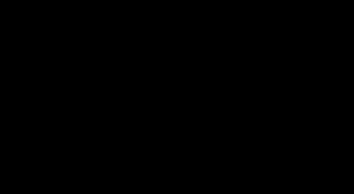
\includegraphics[width=0.7\linewidth]{optocoupler_clearance.pdf}
          \caption{K pojmu external creepage a clearance}
          \label{es:fig_optocoupler_clearance}
        \end{figure}

%} % tikzset
%---------------------------------------------------------------------------------------------------
%=============== Seznam literatury ===============================================================
\printbibliography[title={Seznam literatury}, heading=bibliography]
}  % DEBUG was off
%--------------------------------------------------------------------------------------------------
%                            /$$      /$$  /$$$$$$   /$$$$$$          /$$   /$$                                   | $$$    /$$$ /$$__  $$ /$$__  $$
%                           | $$$    /$$$ /$$__  $$ /$$__  $$        | $$$ | $$                                   | $$$$  /$$$$| $$  \ $$| $$  \__/
%                           | $$$$  /$$$$| $$  \ $$| $$  \__/        | $$$$| $$                                   | $$ $$/$$ $$| $$$$$$$$| $$ /$$$$
%                           | $$ $$/$$ $$| $$$$$$$$| $$ /$$$$ /$$$$$$| $$ $$ $$                                   /$$      /$$  /$$$$$$   /$$$$$$ 
%                           | $$  $$$| $$| $$__  $$| $$|_  $$|______/| $$  $$$$                                   | $$  $$$| $$| $$__  $$| $$|_  $$
%                           | $$\  $ | $$| $$  | $$| $$  \ $$        | $$\  $$$                                   | $$\  $ | $$| $$  | $$| $$  \ $$
%                           | $$ \/  | $$| $$  | $$|  $$$$$$/        | $$ \  $$                                   | $$ \/  | $$| $$  | $$|  $$$$$$/
%                           |__/     |__/|__/  |__/ \______/         |__/  \__/                                   |__/     |__/|__/  |__/ \______/                    
%--------------------------------------------------------------------------------------------------
\ifthenelse{ \equal{\DebugMode}{true} }{% Debug mode ON
  % !TeX spellcheck = cs_CZ
%file:spojity_model_elmag_p.tex
%{\tikzset{external/prefix={tikz/TEO/}}
% \tikzset{external/figure name/.add={ch01_}{}}
%==============================Kapitola: Spojité matematické modely jednotlivých polí ==============
\chapter{Spojité matematické modely polí}
\minitoc
  \section{Elektromagnetické pole}       
    \subsection{Veličiny elektromagnetického pole a jejich jednotky}
      \fbox{Elektrický náboj} je \emph{skalární veličinou}. Jednotkou je \emph{coulomb [C]}. Má
         kvantový charakter (tj. je roven celistvému násobku elementárního náboje $e =
         1,602\cdot10^{-19}C$), avšak v technických aplikacích k tomu nepřihlížíme. Náboj $Q$
         může být rozložen:
         \begin{itemize}\addtolength{\itemsep}{-0.5\baselineskip}
            \item \emph{prostorově} v objemu $V$ s objemovou hustotou
               \begin{equation}\label{TEMP:eq_q_varrho}
                  \varrho = \frac{dQ}{dV} \qquad [C\cdot m^{-3}]
               \end{equation}               
            \item \emph{plošně} na ploše $S$, s plošnou hustotou
               \begin{equation}\label{TEMP:eq_q_sigma}
                  \sigma = \frac{dQ}{dS} \qquad [C\cdot m^{-2}]
               \end{equation}                 
            \item \emph{lineárně} na křivce $l$, s lineární hustotou
               \begin{equation}\label{TEMP:eq_q_tau}
                  \tau = \frac{dQ}{dl} \qquad [C\cdot m^{-1}]
               \end{equation}                 
         \end{itemize}
         Rozlišujeme:
           \begin{itemize}\addtolength{\itemsep}{-0.5\baselineskip}
             \item \textbf{volné náboje}: mohou se přemisťovat v makroskopických
             vzdálenostech,
             \item \textbf{vázané náboje}: mohou se přemisťovat jen v
             mikroskopických vzdálenostech.
           \end{itemize}
         Volnými náboji jsou volné elektrony v kovech nebo ionty v elektrolytech (jsou odpoutány od
         atomů, resp. molekul a volně se mezi nimi pohybují); vázané náboje vznikají polarizací
         dielektrika.
         
      \vspace{1em}
      \fbox{Elektrický proud}\label{TEMP:kap_el_proud_velicina} je znám z každodenního života,
        přesto je velmi důležité umět tento pojem vnímat jak pro označení „jevu“ (kap.
        \ref{TEMP:kap_elproud_jev}), tak jako fyzikální veličinu, která tento jev kvantitativně
        popisuje (kap. \ref{TEMP:kap_el_proud_velicina} ). Elektrický proud je \emph{skalární
        fyzikální veličina} tzn. $I$ resp. $i$, jejíž jednotkou je základní jednotka soustavy SI:
        \emph{ampér} – [A]. V této soustavě jednotek je ampér definován na základě silových
        účinků mezi dvěma vodiči, kterými prochází elektrický proud. Tato síla je magnetického
        původu, avšak magnetické pole vzniká jako důsledek pohybu elektrického náboje.Je tvořen
        uspořádaným pohybem elektrických nábojů.
        
        Připojíme-li vodič ke zdroji elektrického napětí, elektrické pole uvnitř působí elektrickou
        silou na vodivostní elektrony, vyvolává jejich pohyb a tím vytváří elektrický proud, který
        je po krátké době \emph{stacionární} (ustálený, nezávislý na čase). Jestliže vodičem projde
        náboj $\Delta Q$ resp. $dQ$ za časový interval $\Delta t$ resp. $dt$, lze definovat
        \emph{průměrný} resp. \emph{okamžitý} proud ve vodiči:
        \begin{itemize}\addtolength{\itemsep}{-0.5\baselineskip}
          \item \textbf{průměrný} elektrický proud: $$I_{AV} = \frac{\Delta Q}{\Delta t}
                \qquad[A],$$
          \item \textbf{okamžitý} elektrický proud (který je limitním případem proudu průměrného,
                studujeme-li množství náboje, které projde průřezem vodiče za infinitezimální
                (nekonečně krátký) časový interval): $$i = \lim_{\Delta t \rightarrow 0}\frac{\Delta
                Q}{\Delta t} = \frac{dQ}{dt} \qquad[A].$$ V ustáleném stavu protéká všemi průřezy
                vodiče stejně velký proud,
          \item speciálně pohybuje-li se náboj vodičem rovnoměrně, nazýváme proud
                \textbf{stejno\-směr\-ným}, $I(t) = \text{konst}$, a platí $$ I_{DC} =
                \frac{Q}{t}\qquad[A] $$
        \end{itemize}        

        Elektrický proud jako \emph{jev} charakterizuje jednu z forem fyzikálního pohybu, kterou je
        \textbf{uspořádaný pohyb elektricky nabitých částic} v látce. Přestože jakýkoliv elektrický
        proud je vždy tvořen pohybujícími se náboji, nemusí všechny pohybující se náboje vytvářet
        elektrický proud. Ve vodiči dochází ke vzniku trvalého elektrického proudu za těchto
        podmínek:
          \begin{itemize}\addtolength{\itemsep}{-0.5\baselineskip}
            \item vodič se musí nacházet v trvalém elektrickém poli, což je realizováno pomocí tzv.
                  \emph{zdroje} (generátoru) elektrického napětí,
            \item ve vodiči musí být přítomny volné nosiče elektrického náboje.
          \end{itemize}
        
        Podle charakteru vnějšího elektrického pole lze rozlišit tři základní druhy proudů:
          \begin{labeling}{stejnosměrný}\addtolength{\itemsep}{-0.5\baselineskip}
            \item[\textbf{stejnosměrný}] proud vzniká tehdy, jestliže má intenzita elektrického pole
                   konstantní orientaci,
            \item[\textbf{střídavý}] proud ve vodiči vytváří vnější elektrické pole, jehož intenzita
                  periodicky mění svou orientaci na opačnou,
            \item[\textbf{stacionární}] stejnosměrný proud vzniká ve vodiči, je-li intenzita
                  elektrického pole konstantní co do velikosti, směru i orientace.
          \end{labeling}  

       Nabité částice představující volný náboj ve vodičích jsou v neustálém chaotickém tepelném
       pohybu (viz molekulová fyzika a termodynamika). Jedná se o \emph{mikroskopický pohyb}, který
       nemá za následek makroskopicky pozorovatelné přemístění náboje. Pokud ve vodiči vytvoříme
       elektrické pole, tepelný pohyb nabitých částic neustane, ale k náhodné složce rychlosti
       přibude ještě složka rychlosti ve směru vloženého pole.
       
       Při studiu elektrického proudu v kovových vodičích se zabýváme ustálenými proudy
       vodivostních elektronů, které v kovu vytváří tzv. \emph{elektronový plyn}. Tyto vodivostní
       elektrony jsou téměř volné a pohybují se v poli kladných iontů uspořádaných v krystalové
       mřížce.
        
       Experimentálně lze elektromagnetické pole prokázat silovým působením na elektricky nabité
       částice. Celkovou sílu $\vec{F}$ lze rozložit na elektrickou sílu $\vec{F}_e$, nezávislou na
       tom, zda je nabitá částice v klidu nebo v pohybu vůči vztažné soustavě a na magnetickou sílu
       $\vec{F}_m$, působící jen na pohybující se částice. Elektromagnetické pole má tedy dvě
       složky: \textbf{elektrické pole}, působící na náboj silou $\vec{F}_e$ a \textbf{magnetické
       pole}, působící na pohybující se náboj silou $\vec{F}_m$  \cite[s.~13]{Mayer2001}.
      
      \vspace{1em}
      \fbox{Intenzita elektrického pole $\vec{E}$} je vektorovou veličinou charakterizující
        \emph{elektrické pole}.
        Je definována jako 
        \emph{síla působící na nepohybující se jednotkový bodový náboj}:
        \begin{equation}\label{TEMP:eq_E}
          \vec{E} = \frac{\vec{F}_e}{Q} \qquad\left[\frac{V}{m}\right]  
        \end{equation}        
        kde $\vec{F}_e$ je elektrická síla působící na náboj $Q$.
      
      \vspace{1em}
      \fbox{Magnetická indukce $\vec{B}$} je vektorovou veličinou charakterizující \emph{magnetické
        pole}. Je definovována vztahem
        \begin{equation}\label{TEMP:eq_B}
          \vec{F}_m = Q(\vec{v}\times\vec{B}) \qquad[T]  
        \end{equation}        
        kde $\vec{F}_m$ je magnetická síla působící na náboj $Q$ pohybující se rychlostí $\vec{v}$.
        Jednotkou je \emph{tesla} $[T]$.
    
        Síla, jež působí elektromagnetické pole na pohybující se náboj se nazývá \textbf{Lorentzova
        síla}
        \begin{equation}\label{TEMP:eq_Lorentz}
          \vec{F} = \vec{F}_e + \vec{F}_m =Q(\vec{E} + \vec{v}\times\vec{B}) \qquad[N]  
        \end{equation}        

    \subsection{Maxwellovy rovnice}
      Makroskopická teorie elektromagnetického pole v klasickém pojetí vychází ze základních zákonů
      vyjádřených \emph{Maxwellovými rovnicemi (MR)}. Lze je zapsat buď v \textbf{integrálním},
      nebo \textbf{diferenciálním tvaru}. V integrálním tvaru popisují elektromagnetické pole v
      jisté prostorové oblasti $\Omega$, kdežto v diferenciálním tvaru ve vnitřním bodě této
      oblasti. Soustavu vlastních MR představují první čtyři páry rovnic; často se k nim připojuje
      jako další základní rovnice elektromagnetického pole rovnice kontinuity pro vodivý proud.
      Její integrální a diferenciální tvar reprezentují poslední dvě rovnice.
exa
      \begin{align}
        \oint_\mathcal{C}\vr{H} d\vr{l} &= I+\der{\Psi}{t}
                                           \quad \rot{H}=\vr{J}+\pder{\vr{D}}{t}             \\
        \oint_\mathcal{C}\vr{E} d\vr{l} &= -\der{\Phi}{t}
                               \qquad \rot{E}=-\pder{\vr{B}}{t}\\
         \int_\mathcal{S}\vr{D} d\vr{S} &= Q \qquad\quad\;   \diver{D}=\rho_V                \\
         \int_\mathcal{S}\vr{B} d\vr{S} &= 0 \qquad\quad\;\; \diver{B}=0                     \\
         \int_\mathcal{S}\vr{J} d\vr{S} &= -\der{Q}{t} \quad\;\;\;\diver{J}=-\der{\rho_V}{t}
      \end{align}

      Předpokládá se, že \emph{všechny křivky a plochy v integrálním tvaru MR jsou po částech
      hladké a všechny integrované veličiny jsou po částech spojité funkce}. Pak je zaručena
      existence integrálů v těchto rovnicích. V diferenciálním tvaru MR se předpokládají pouze
      \textbf{regulární body} oblastí, což jsou body, v nichž jsou veličiny $\vr{E}$, $\vr{D}$,
      $\vr{B}$ a $\vr{H}$ \emph{spojité a spojitě diferencovatelné funkce}; nejsou jimi tedy např.
      body rozhraní dvou různých prostředí, v elektrickém poli body v nichž jsou umístěny diskrétní
      náboje, v magnetickém poli body proudových vláken atd.

      % --------example: Energie v Kondenzátoru ------------------------
      % \label{TEO:exam019}
      % !TeX spellcheck = cs_CZ
\begin{example}\label{teo:exam019}
  Mějme nabitý deskový kondenzátor \(C\), zobrazený na obr. \ref{teo:fig019a}. Zvětšme jeho
  kapacitu, například tím, že zvětšíme plochu jeho elektrod, nebo připojíme paralelně druhý stejné 
  velikosti, viz obr. \ref{teo:fig019b}. Otázka zní, jak velká enerige bude uložena v 
  elektrostatickém poli obou kondeznátorů? Bude energie po rozdělení náboje mezi oba 
  kondenzátory rovna původní energií nabitého kondenzátoru? Pokud ne, vysvětlete kam se část 
  energie transformovala. 
  
   {\centering
    \captionsetup{type=figure}
    \begin{tabular}{cc}
     \subfloat[ ]{\label{teo:fig019a}
       \includegraphics[width=0.15\linewidth]{teo_fig019a.png}}              &
     \hspace{3em}
     \subfloat[ ]{\label{teo:fig019b}
       \includegraphics[width=0.5\linewidth]{teo_fig019b.png}}
    \end{tabular}
    \captionof{figure}{K příkladu \ref{teo:exam019}: a) Nabitý kondenzátor s rovnoběžnými rovinnými 
    elektrodami; b) Rozložení náboje na obou kondenzátorech velikosti}
    \label{teo:fig019}
  \par}
  
  Je-li dielektrikum kondenzátoru lineární, pak pro energii elektrického pole akumulovanou v 
  nabitém kondenzátoru platí. Podrobněji například v kapitole \ref{fyz:IIchapVsecXIX}.
  \begin{equation}
    W = \frac{1}{2}CU^2 \quad\text{nebo}\quad W = \frac{1}{2}\frac{Q^2}{C} 
    \quad\text{kde}\quad C = \frac{Q}{U}
  \end{equation}
  Předpokládejme ustálený stav po připojení druhého kondenzátoru, jak je znázorněno na obr. 
  \ref{teo:fig019b}. V obvodu nepředpokládáme přítomnost odporu, který by způsobil ztrátu energie, 
  vyzářené v podobě tepla. Kapacita je dvojnásobná a náboj zůstal stejný. Na každém kondenzátoru 
  tedy očekáváme polovinu původního náboje. Sečteme-li energii uloženou v elektrických polích obou 
  kondenzátorů dostaneme
  \begin{align*}
    W^* &= \frac{1}{2}\frac{(\frac{1}{2}Q)^2}{C} + \frac{1}{2}\frac{(\frac{1}{2}Q)^2}{C} 
         = \frac{(\frac{1}{2}Q)^2}{C} =\frac{1}{4}\frac{Q^2}{C}                               \\
        &  \xrightarrow[\scriptscriptstyle{C\rightarrow2C}]{}
           \frac{1}{2}\frac{Q^2}{(2C)} = \frac{1}{2}W 
  \end{align*}
  Kupodivu, polovina energie prostě chybí a jelikož platí zákon zachování energie\footnote{viz 
  partie Fyzika \ref{part:FYZI}, kapitola \ref{fyz:IchapII})}, nezbývá nic jiného než uznat, že 
  elektrický obvod dle \ref{teo:fig019b}, nemodeluje fyzikální problém dost věrně. Tím jsme dospěli 
  k závěru, že je nutné do obvodu dodat rezistor, tak jak je znázorněno na obrázku   
  \ref{teo:fig020}.
  
   {\centering
    \captionsetup{type=figure}
    \includegraphics[width=0.4\linewidth]{teo_fig020.png}
    \captionof{figure}{Rezistor \(R\) představuje ztráty, které nebyly v obvodu na obrázku 
               \ref{teo:fig019b} předpokládány}
    \label{teo:fig020}
  \par}
  
  Abychom mohli určit teplné ztráty na rezistoru dané integrálem \(\int_{0}^{\infty} 
  Ri^2(t)\dd{t}\), nedříve sestavíme jednoduchou diferenciální rovnici prvního řádu aplikací II. 
  Kirchhoffova zákona, ze které odvodíme vzorec pro časovou závislost proudu \(i(t)\). 
  \begin{align*}
    \frac{Q_0 - Q}{C} - Ri(t) - \frac{Q_0}{C}         &= 0 \quad/\der{ }{t}             \\
    \frac{-i(t)}{C} - R\der{i(t)}{t} - \frac{i(t)}{C} &= 0                              \\
                                        \der{i(t)}{t} &= - \frac{2}{RC}i(t) \quad/\int  \\
                                                 i(t) &= I_0e^{-\frac{2}{RC}t}
  \end{align*}
  Nyní můžeme stanovit energii disipované na rezitoru \(R\)
  \begin{align*}
    W   &= \int_{0}^{\infty}Ri^2(t)\dd{t} = RI_0^2\int_{0}^{\infty}e^{-\frac{4}{RC}t}\dd{t}   \\
    \shortintertext{Do integrované funkce dosadíme novou proměnnou \(u = \frac{4}{RC}t\), \(\dd{u} 
                    = \frac{4}{RC}\dd{t}\), \(\dd{t} = \frac{RC}{4}\dd{u}\)}
        &= RI_0^2\int_{0}^{\infty}e^{-u}\frac{RC}{4}\dd{u} 
         = R^2I_0^2\frac{C}{4}\underbrace{\int_{0}^{\infty}e^{-u}\dd{u}}_1  \\
    \shortintertext{Jelikož platí \(I_0 = \frac{U}{R}=\frac{Q}{CR}\) dostaneme po dosazení}
        &= \cancel{R^2}\frac{Q^2}{C^2\cancel{R^2}}\frac{C}{4} = \frac{Q^2}{4C}
         = \frac{1}{2}W
  \end{align*}
  Nyní je vše v pořádku. Druhá polovina energie je disipována na rezistoru a navíc z výsledku 
  vyplývá, že vubec nezávisí na \(R\)!
\end{example}


  
      %-----------------------------------------------------------------
      
  % --------------- Stacionární magnetické pole-----------------------------------------------------
  \section{Stacionární proudové pole}
    V elektrostatice (tj. elektrickém poli nepohybujících se nábojů) neexistuje trvalý elektrický
    proud. Zdroje napětí (galvanické články, termočlánky, dynama aj.) mají tu vlastnost, že na
    jejich záporné svorce je trvale nadbytek elektronů, a na jejich kladné svorce jejich
    nedostatek. Těmito zdroji můžeme ve vodiči trvale udržovat elektrické pole a tedy i tok nosičů
    elektřiny. Jestliže se \emph{náboje pohybují konstantní rychlostí, hovoříme o stacionárním
    elektrickém proudu}. Základní rovnice elektrostatické pole jsou:

    \begin{table}[ht!]
      \setlength\extrarowheight{5pt}
      \centering
      \begin{tabular}{lc|c|}
        \cline{2-3}
        \multicolumn{1}{l|}{} 
          & \textbf{integrální tvar} & \textbf{diferenciální tvar}                    \\[8pt]
        \hline
        \multicolumn{1}{|l|}{2. MR} 
          & \(\bigointsss\vr{E}\cdot d\vr{l} = 0\) & \(\rot{E} = 0\)                  \\[8pt] 
        \cline{1-3}
        \hline
        \multicolumn{1}{|l|}{Zákon kontinuity} 
          & \(\bigointsss\vr{J}\cdot d\vr{S}=0\) & \(\diver{J}=0\)                    \\[8pt]
        \cline{1-3}
        \multicolumn{1}{|l|}{Ohmův zákon}
          & \(I=GU=\dfrac{U}{R}\) & \(\vr{J} = \gamma\vr{E} = \dfrac{1}{\rho}\vr{E}\) \\[8pt]
        \cline{1-3}
      \end{tabular}
      \caption{Základní rovnice stacionárního proudového pole}
    \end{table}
    
    \subsection{Elektrický proud v kovových vodičích}\label{TEMP:kap_elproud_jev}
      V předchozí kapitole \ref{TEMP:kap_el_proud_velicina} bylo o elektrickém proudu pojednáváno
      jako o skalární fyzikální veličině. V této kapitole nás bude zajímat makroskopický pohled na
      „jev“ známý jako \emph{elektrický proud}.
      
      Zopakujme, že elektrickým proudem je míněn uspořádaný pohyb elektrických ná\-bo\-jů, a aby se
      tyto náboje mohly pohybovat, musí být volné - jsou přítomny v látkách, které nazýváme
      \textbf{vodiče}. Vodiče mohou mít nositele náboje jednoho znaménka (elektrony v kovech,
      uhlíku a v polovodičových) anebo obojích znamének (kladné a záporné ionty v elektrolytech,
      ionty a elektrony v ionizovaných plynech). Volné nositele náboje (elektrony, ionty) lze
      rovněž oddělit od těchto látek (vodičů) a vytvořit elektrický proud ve vakuu nebo ve
      zředěných plynech.
      
      Z vodičů mají největší význam \textbf{kovy}, které jsou polykrystalickými látkami s kovovou
      vazbou. Každý mikroskopický monokrystal kovu má pevnou krystalovou mříž sestavenou z kladných
      iontů, mezi nimiž se přetržitě pohybují \emph{volné elektrony} rychlost\-mi, jejichž velikost
      je statisticky proměnná (co do velikosti i směru). Střední hodnota rychlosti (jako vektoru)
      všech elektronů je nulová. Střední hodnota rychlosti určitého elektronu je závislá na teplotě
      vodiče. Elektrony konají tzv. \emph{termický pohyb}. Rychlosti neuspořádaných termických
      pohybů dosahují jen o několik řádů větších hodnot, než kmity iontů v krystalech mřížky.

      \begin{figure}
        \centering
        \includegraphics[width=0.5\linewidth]{vd_e_drift.pdf}
        \caption[Pohyb elektronu ve vodiči.]{Pohyb elektronu ve vodiči. Fyzikálně je $v_d$ 
                 průměrná rychlost nosičů náboje uvnitř vodiče, který je vložen do vnějšího
                 elektrického pole. Ve skutečnosti se ale elektron ve vodiči nepohybuje po přímce,
                 jeho pohyb je chaotický.}
        \label{TEMP:fig_vd_e_drift}
      \end{figure}
      
      Připojíme-li vodič k vnějšímu zdroji elektrického pole (např. ke galvanickému článku), začne
      statisticky převládat uspořádaný pohyb nosičů kladného (záporného) náboje ve směru (proti
      směru) vnějšího pole nad termickým pohybem, což v makroskopickém měřít\-ku pozorujeme jako
      \textbf{makroskopický elektrický proud}. Jsou-li ve vodiči přítomny nosiče náboje obou
      polarit, dojde k pohybu ve vzájemně opačných směrech, přičemž směr toku nosičů kladného
      náboje se historicky ztotožňuje se směrem toku elektrického proudu. U kovových vodičů je tedy
      směr proudu právě opačný, než směr toku elektronů, jenž tento elektrický proud tvoří.
      
      Velikost (intenzitu) proudu posuzujeme podle velikosti náboje obojí polarity, který projde
      určitým průřezem vodiče ve vzájemně opačných směrech za jednotku času. Projde-li průřezem
      vodiče celkově náboj $dQ$ za čas $dt$, bude tok náboje vodičem charakterizovat skalární
      veličina
        \begin{equation}\label{TEMP:eq_I_01}
          I = \frac{dQ}{dt} \qquad[A],  
        \end{equation}        
      která se nazývá \emph{elektrický proud}($1C\cdot s^{-1} = 1A $ čteno \emph{ampér}). Tato
      jednotka patří mezi základní jednotky \texttt{SI} soustavy.
      
      Pro \emph{stacionární} (tj. časově neproměnný - ustálený) proud můžeme obecný výraz
      \ref{TEMP:eq_I_01} nahradit rovnicí
        \begin{equation}\label{TEMP:eq_I_02}
          I = \frac{Q}{t}.  
        \end{equation}       
      Jedná-li se o rovnoměrný pohyb bodového náboje $Q$ po kružnici s periodou $T$, resp. s
      úhlovou rychlostí $\omega$, můžeme vzniklý ustálený proud vyjádřit rovnicí 
        \begin{equation}\label{TEMP:eq_I_03}
          I = \frac{Q}{T} = \frac{\omega Q}{2\pi}.  
        \end{equation}
      
      Bude-li se element náboje $dQ$ pohybovat v lineárním útvaru rychlostí $v = \frac{dQ}{dl}$,
      bude po dosazení do rov.\ref{TEMP:eq_I_01} reprezentovat elektrický proud 
        \begin{equation}\label{TEMP:eq_I_04}
          I = \frac{dQ}{dt} = \frac{dQ}{dl}v = \tau v, 
        \end{equation}      
      kde $\tau$ je \emph{délková hustota} náboje a $v$ je velikost \emph{okamžité rychlosti}
      náboje v uvažovaném místě lineárního útvaru. 

      \begin{figure}[ht!]
         \centering
         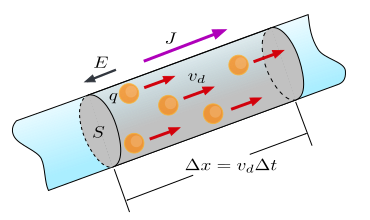
\includegraphics[width=0.5\linewidth]{el_proud_ve_vodici.pdf}
         \caption[Náboje, pohybující se vodičem]{Směr elektrického proudu byl implicitně stanoven
                  jako směr pohybu kladných nábojů. Nositeli elektrického náboje uvnitř vodičů jsou
                  ovšem záporně nabité volné elektrony, které se tedy dle  konvence pohybují proti
                  směru elektrického proudu. Elektrický proud může protékat pevnými látkami (kovy,
                  polovodiči), kapalinami (elektrolyty) a ionizovanými plyny. Látky, které nevedou
                  elektrický proud, nazýváme nevodiči, izolanty}
         \label{TEMP:fig_el_proud_ve_vodici}
      \end{figure}
      
      Elektrický proud je veličina, která obecně popisuje prostorový jev. Omezíme se nyní na běžný
      případ vodiče, jako je na obr. \ref{TEMP:fig_el_proud_ve_vodici}, který má volné náboje jen
      jedné polarity (u kovových vodičů jde o elektrony) a označme $\rho_0$ prostorovou hustotu
      volného náboje a $v_d$ velikost usměrněné rychlosti jejich nositelů (elektronů). Pak za čas
      $dt$ projde průřezem o obsahu $S_0$ ($S_0\bot v_d$) náboj $dQ = \rho_0 S_0 v_d dt$.
      Elektrický proud vyjádřený rov.
      \ref{TEMP:eq_I_01} můžeme přepsat do tvaru
        \begin{equation}\label{TEMP:eq_I_05}
          I = \rho_0 S_0 v_d = - e n_0 S_0 v_d, 
        \end{equation}         
      kde $\displaystyle{n_0 = \frac{\rho_0}{-e}}$ je počet nositelů volného náboje (tj. v našem
      případě elektronů, z nichž každý nese náboj $-e$ v jednotkovém objemu vodiče, přičemž pro
      elektrony zřejmě je $\rho_0<0$.

      \begin{wrapfigure}[14]{r}{5cm}
        \centering
        \includegraphics[width=0.9\linewidth]{plocha_S.pdf}
        \caption[Rovinná plocha $S$.]{Rovinná plocha $S = S_0\cos\alpha$}
        \label{TEMP:fig_plocha_S}
      \end{wrapfigure}
      Rovinnou plochou $S$ průřezu můžeme zavést jako vektor $vr{S}$, který má směr daný normálou k
      ploše a pravidlem pravé ruky (ukazují-li prsty pravé ruky směr oběhu po hraniční křivce
      plochy, ukáže palec směr plochy jako vektoru $\vr{S}$). Protože driftová rychlost $v_d$ je
      také vektor, nebudeme obecně uvažovat vektory $\vr{S}, \vr{v_d}$ o stejném směru a rovnici
      \ref{TEMP:eq_I_05} přepíšeme do obecnějšího tvaru      
      
      \begin{equation}\label{TEMP:eq_I_06}
        I = \rho_0 \vr{S_0}\cdot\vr{v}_d = jS\cos\alpha = jS_0, 
      \end{equation}      
      kde $S_0 = S$ pro $\alpha = 0$ (viz obr. \ref{TEMP:fig_plocha_S}) a   
      \begin{equation}\label{TEMP:eq_I_07}
        \vr{j} = \rho_0\vr{v_d}, 
      \end{equation}        
      je proudová hustota. Je to vektor o velikosti 
      \begin{equation}\label{TEMP:eq_I_08}
        j = \frac{I}{S\cos\alpha} = \frac{I}{S_0}  \qquad A\cdot m^{-2}, 
      \end{equation}   
      obecněji
      \begin{equation}\label{TEMP:eq_I_09}
        j = \frac{dI}{dS}, 
      \end{equation}

      a o směru vektoru driftové rychlosti nositelů kladného náboje. Pro případ nositelů volného
      náboje - elektronů má proudová hustota opačný směr než driftová rychlost $v_d$ (obr.
      \ref{TEMP:fig_plocha_S}).
      
      Velikost vektoru $\vr{j}$ má význam plošné hustoty elektrického proudu v uvažovaném místě
      průřezu. Jednotkou je $A\cdot m^{-2}$.
      
      Nebude-li proudová hustota na uvažovaném průřezu konstantní, bude celkový elektrický proud
      procházející průřezem o obsahu $S$ dán integrálem 
        \begin{equation}\label{TEMP:eq_I_10}
          I = \int_S \vr{j}d\vr{S}. 
        \end{equation} 

      % --------example: Driftová rychlost elektroknů ve vodiči --------
      % \label{TEO:exam008}
      % !TeX spellcheck = cs_CZ
%---------- Driftová rychlost elektroknů ve vodiči: 
\begin{mdframed}[style=mdexam]
\begin{example}\label{TEO:exam008} \emph{Driftová rychlost elektronů ve vodiči:} Vodičem z 
jednomocné mědi o
  průřezu $S_0 = \SI{1}{\mm^2}$ prochází elektrický proud $I = \SI{5}{\A}$. Vypočtěte:
  \begin{itemize}[noitemsep, leftmargin=2em]
    \item počet volných elektronů v jednotkovém objemu \ce{Cu},
    \item úhrnný náboj volných elektronů v jednotkovém objemu,
    \item driftovou rychlost volných elektronů při proudu \(I\).
  \end{itemize}
  Měď má poměrnou atomovou hmotnost $A_r = 63,54$ a hustotu\footnote{Pro hustotu budeme používat 
  alternativní značku $s$, s ohledem na kolizi značky $\rho$, jež označuje hustotu náboje.} $s = 
  \SI{8.93e3}{\kg.\m^{-3}}$.\newline  
  \textbf{Řešení:}
  \begin{itemize}[leftmargin=2em]
    \item Jeden mol mědi o molové hmotnosti $M = \SI{0.06354}{\kg\per\mol}$ a o molovém
          objemu 
          \begin{align*}
            V_m &= \frac{M}{s} 
                 = \frac{\SI{63.54e-3}{\kg.\mol^{-1}}}{\SI{8.93e3}{\kg.\m^{-3}}}      \\
                &= \SI{7.12e-6}{\m^3.\mol^{-1}}
          \end{align*}
          obsahuje $N_A = 6,0221\cdot10^{23}$ jednoatomových molekul \emph{Cu} na jeden mol,
          z nichž každý má volný jeden (valenční) elektron. Tedy počet volných elektronů v
          jednotkovém objemu je 
          \begin{align*}
            n_0 &= \frac{N_A}{V_m} = \frac{sN_A}{M}                                           
                 = \frac{\SI{6.0221e23}{\mol^{-1}}}{\SI{7.12e-6}{\m^{3}.\mol^{-1}}}    \\
                &= \SI{8.46e28}{\per\cubic\m}.
          \end{align*}  
    \item Úhrnný náboj volných elektronů v jednotkovém objemu mědi je 
          \begin{equation}
            Q_v = -e\cdot n_0 = \SI{-1.36e10}{\coulomb.m^{-3}}.
          \end{equation}
    \item Velikost driftové rychlosti určíme ze vztahu $I = -en_0v_dS_0 = - Q_v v_d S_0$ tj.
    \begin{align*}
      v_d &= \left\lvert\frac{I}{Q_v\cdot S_0}\right\rvert                       
           = \frac{\SI{5}{\coulomb\per\s}}{\SI{1.36e10}{\coulomb.m^{-3}}\cdot\SI{1e-6}{\m^2}}   \\
          &= \SI{3676e-4}{\m\per\s} = \SI{0.3676}{\mm\per\s}.  
    \end{align*}
  \end{itemize}
  Z provedených výpočtů si můžeme udělat názor o mikroskopických poměrech v kovových vodičích: počet
  volných nositelů náboje - elektronů a jejich úhrný náboj v jednotkovém objemu je značný a proto
  driftová rychlost elektronů potřebná k vyvolání proudu běžné velikosti v drátových vodičích je
  nesmírně malá (doslova hlemýždí).
\end{example}  
\end{mdframed}
  
      %-----------------------------------------------------------------

      % --------example: Velikost náboje v minci -----------------------
      % \label{TEO:exam009}
      % !TeX spellcheck = cs_CZ
%---------- Velikost náboje v minvi:
\begin{example}
  Elektricky neutrální měděná mince o hmotnosti \(m = \SI{3.11}{\g}\) obsahuje stejné množství 
  kladného a záporného náboje. Jaké je velikost kladného (nebo záporného) náboje obsaženého v 
  minci?\newline  
  \textbf{Řešení:}\newline
  Neutrální atom má záporný náboj \(Z\cdot e\), představovaný jeho elektrony a kladný náboj o 
  stejné velikosti představovaný protony v jádře. Pro měď je atomové číslo \(Z\) rovno \num{29}, 
  tj. atom mědi má \num{29} protonů, a je-li elektricky neutrální, také \num{29} elektronů.
  
  Náboj o velikosti \(Q_v\), který hledáme je roven \(N\cdot Z\cdot e\), kde \(N\) je počet atomů 
  obsažených v  jednom molu (Avogadrova konstanta: \(N_A = \SI{6.0221e23}{\per\mole}\)). Počet 
  molů mědi v minci \(\frac{m}{M}\), kde \(M = \SI{63.5}{\g\per\mole}\) je molární hmotnosti mědi: 
  \begin{equation*}
    N = N_A\cdot\frac{m}{M} = \SI{6.0221e23}{\per\mole}
           \frac{\SI{3.11}{\g}}{\SI{63.5}{\g\per\mole}} 
      = \num{2.95e22}.
  \end{equation*}
 Velikost celkového kladného (záporného) náboje v minci je pak 
  \begin{equation*}
    Q_v = N\cdot Z\cdot e = \num{2.95e22}\cdot\num{29}\cdot\SI{1.602e-19}{\coulomb} 
        = \SI{137039}{\coulomb}
  \end{equation*}
  To je obrovský náboj. Pro srovnání: třeme-li ebonitovou tyč vlněnou látkou, můžeme na tyč 
  přemístit stěží náboj o velikosti \SI{1e-9}{\coulomb}.
\end{example} 
  
      %-----------------------------------------------------------------

    % ----------------Práce a výkon elektrického proudu-----------------
    \subsection{Práce a výkon elektrického proudu}
      % --------example: Ponorný vařič ---------------------------------
      % \label{TEO:exam010}
      % !TeX spellcheck = cs_CZ
%---------- Ponorný vařič:
\begin{mdframed}[style=mdexam]
  \begin{example}\label{TEO:exam010}
    Za jakou dobu uvede norný vodič o příkonu \SI{600}{\W} do varu \SI{1}{\litre} vody o počáteční
    teplotě $\SI{20}{\degreeCelsius}$. Uvažujte měrnou tepelnou kapacitu vody $c =
    \SI{4200}{\joule\per\kg\per\K}$. Výměnu tepla s okolím neuvažujte.
    \newline 
    \textbf{Řešení:}\newline Pro var vody bude zapotřebí tepla dle rovnice $Q  = m\cdot c\cdot(T_2 -
    T_1)$. Potřebná elektrická práce je $Q_e = P\cdot t = U\cdot I\cdot t$ a tedy dobu ohřevu
    stanovíme z rovnice:
    
    {\centering
    \captionsetup{type=figure}
    \luafigure[0.3]{teo_fig033.png}
    \captionof{figure}{Ilustrace k příkladu \ref{TEO:exam010}}
    \label{teo:fig033}
    \par}

    \begin{align*}
      P\cdot t &= m\cdot c\cdot(T_2 - T_1)                                               \\
             t &= \frac{m\cdot c}{P}\cdot(T_2 - T_1)                                     \\     
               &= \frac{\SI{1}{\kg}\cdot\SI{4200}{\joule\per\kg\per\K}}{\SI{600}{\W}}
                \cdot(\SI{100}{\degreeCelsius} - \SI{20}{\degreeCelsius})                \\ 
               &= \SI{560}{\s}.
    \end{align*}         
  \end{example}
\end{mdframed}  
      %-----------------------------------------------------------------
 
    % ----------------Ohmův zákon------------------------------------------------------------------
    \subsection{Ohmův zákon}
      Uvažujme vodič u něhož jsou volnými nositeli náboje \emph{elektrony}. Nyní v mezích klasické
      mechaniky kvantitativně popíšeme mechanismus vedení proudu, který povede k všeobecně známému
      \textbf{Ohmovu zákonu}
      
      Umístíme-li vodič do elektrického pole o intenzitě $\vec{E}$ (např. připojením ke
      galvanickému článku), působí na každý volný elektron síla $\vec{F} = -e\vec{E}$, která mu
      podle \emph{Newtonova zákona} udělí zrychlení $\vec{a} = \frac{\vec{F}}{m_e} = -
      \frac{e}{m_e}\vec{E}$ proti směru vnějšího pole. Tím získávají chaoticky se pohybující
      elektrony ještě složku rychlosti v protisměru vloženého elektrického pole $\vec{E}$ a  dojde
      tedy k usměrnění driftového pohybu volných elektronů a v souladu s kapitolou
      \ref{TEMP:kap_elproud_jev} pozorujeme, že ve vodiči vznikl makroskopický elektrický proud.
      
      Pohyb elektronu se ovšem neobejde bez srážek s ionty v krystalové mřížce. Dráhu, kterou se
      elektronu podaří urazit, nazýváme \emph{volnou dráhou} $d$. Průměrná doba mezi dvěma po sobě
      jdoucími srážkami nechť je $\tau$ za tuto dobu se bude elektron rovnoměrně urychlovat a těsně
      před následující srážkou jeho rychlost dosáhne maxima tj. $\vec{v}_{max} = \vec{a}\cdot\tau$.
      Nás ovšem zajímá průměrná rychlost (\emph{driftová rychlost})na volné dráze průměrné
      velikosti:
      \begin{equation}\label{TEMP:eq_vd_01}
        \vec{v}_d = \frac{\vec{v}_{max}}{2} = -\frac{e\tau}{2m_e}\vec{E}
      \end{equation}   
      Proudová hustota \ref{TEMP:eq_I_07} bude
      \begin{equation}\label{TEMP:eq_j_02}
        \vec{j} = \rho_0\vec{v}_d= -en_0\vec{v}_d = -\frac{e^2n_0\tau}{2m_e}\vec{E}
      \end{equation}       
      Koeficient úměrnosti 
      \begin{equation}\label{TEMP:eq_g_03}
        \gamma = \frac{e^2n_0\tau}{2m_e}
      \end{equation}     
      je závislý na počtů nositelů (elektronů) $n_0$ v jednotkovém objemu a na době $\tau$, neboli
      na délce volné dráhy. Veličina $\gamma$ se nazývá \emph{měrná elektrická vodivost} neboli
      \textbf{konduktivita} látky. Protože dobu $\tau$ nelze přímo měřit, určuje se $\gamma$
      experimentálně. Přitom se zjišťuje, že pro určitou teplotu zkoumané látky je $\gamma$
      konstantní.
      
      Po zavedení pojmu měrná elektrická vodivost látky \ref{TEMP:eq_g_03}, můžeme výraz
      \ref{TEMP:eq_j_02} přepsat do výsledného tvaru
      \begin{equation}\label{TEMP:eq_j_04}
        \vec{j} = \gamma\vec{E},
      \end{equation}              
      který se v literatuře označuje jako \emph{Ohmův zákon v diferenciálním tvaru} (i když se v
      pravém slova smyslu o diferenciální tvar nejedná). Výstižnější je označení \emph{lokální tvar
      Ohmova zákona}, protože výraz \ref{TEMP:eq_j_04} se vztahuje na určité místo, resp. bod,
      vodivého prostředí. Vztah říká, že proudová hustota v určitém bodě vodivého prostředí je
      přímo úměrná intenzitě vloženého elektrického pole v tomto bodě (platí pro určitou teplotu
      prostředí).
      
      Uvažujme nyní lineární homogenní vodič délky $l$ a příčného průřezu o obsahu $S_0$, připojený
      ke zdroji o napětí $U$. Pak intenzita pole uvnitř vodiče bude mít konstantní velikost
      $E=\frac{U}{l}$. Dosadíme-li za velikost proudové hustoty $j=\frac{I}{S_0}$ do
      \ref{TEMP:eq_j_04}, dostaneme vztah
      \begin{equation}\label{TEMP:eq_j_05}
        \frac{I}{S_0} = \gamma\frac{U}{l},
      \end{equation}        
      z něhož vyplývá známý vztah
      \begin{equation}\label{TEMP:eq_j_06}
        U = \frac{l}{\gamma S_0}I = RI,
      \end{equation}              
      kde
      \begin{equation}\label{TEMP:eq_j_07}
        R = \frac{l}{\gamma S_0} = \rho\frac{l}{S_0},
      \end{equation} 
      je \textbf{elektrický odpor} uvažovaného lineárního vodiče, přičemž $\rho = \frac{1}{\gamma}$
      je \emph{měrný elektrický odpor} (\textbf{rezistivita})\footnote{Zde je další kolize značky
      $\rho$. Nyní se tomuto problému vyhneme využíváním pouze konduktivity, jenž se častěji
      používá v teorii elektromagnetického pole.}. Výraz \ref{TEMP:eq_j_07} představuje klasický
      Ohmův zákon zákon experimentálně objevený r. 1826 \emph{G. S. Ohmem}. Jednotky:
      \begin{itemize}\addtolength{\itemsep}{-0.5\baselineskip}
        \item elektrický odpor: \si{V.A^{-1}},
        \item měrný elektrický odpor: \si{\ohm.m},
        \item měrná elektrická vodivost: \si{\ohm^{-1}.m^{-1}}.
      \end{itemize}

      % --------example: Ponorný vařič -----------------------
      % \label{TEO:exam011}
      % !TeX spellcheck = cs_CZ
\begin{example}
  \textbf{Zemnicí elektroda}: Uvažujte zemnicí elektrodu ve tvaru koule o poloměru  
  $a=\SI{200}{\mm}$, uloženou do zeminy v hloubce, která je značně větší než je poloměr $a$. Pro 
  jednoduchost řešení dále předpokládejte, že přívodní drát je od zeminy izolován (obr.
  \ref{TEMP:fig_zem_elektroda}). Zemina má měrnou vodivost $\gamma=\num[exponent-product =
  \cdot]{1,8e-2}\si{\per\ohm\per\m}$. Při zkratu teče přívodním drátem proud $I=\SI{50}{\A}$.
  Vypočítejte:
  
  %----------------------------------
  % image: TEMP_zem_elektroda.tex label: \label{TEMP:fig_zem_elektroda}
  % \documentclass{article}
% \usepackage{tikz}
% \usetikzlibrary{decorations.markings}
% \usetikzlibrary{intersections}
% \usetikzlibrary{calc}

% \begin{document}
   {\centering  
    \begin{tikzpicture}[scale=0.8, every node/.style={scale=1}]
      \coordinate (pCenter) at (0,-5);
      \fill[brown!60] (-2,-0.2) rectangle (2,-7);
      \draw[color=brown, line width=5pt] (-2,-0.2) -- +(4,0); 
      \draw[->,line width=1pt] (0,1) node[left] {$I$} -- (0,-0.1);        
      \draw[line width=1pt] (0,0) -- (pCenter);
      \draw[line width=1pt,color=black, fill=white]
           (pCenter) circle[radius=0.5];
      \draw[line width=1pt, dotted]
           (pCenter) circle[radius=1];
      \foreach \angle in
          {0, 30, 60, 120, 150, 180, 210, 240, 270, 300, 330}
      {
        \draw[->, line width=0.75pt] (pCenter)++(\angle:1.2) -- +(\angle:0.3);        
      }
      \draw[<->, thick] (pCenter)++(240:1) coordinate(pR) -- (pCenter) -- +(330:0.5) coordinate(pA); 
      \node[above] at ($ (pCenter)!0.5!(pA) $) {$a$};     
      \node[above] at ($ (pCenter)!0.9!(pR) $) {$r$}; 
      \node[above] at (-1,-2) {$\gamma$};
      \node[above] at (+1.5,-4.5) {$\vec{j}$};
    \end{tikzpicture}
    \captionsetup{type=figure}
    \captionof{figure}{Zemnicí elektroda}
    \label{TEMP:fig_zem_elektroda}
  \par}
  
% \end{document}    
  %----------------------------------         
  \begin{enumerate}[label=\emph{\alph*})]
    \item Závislost potenciálu $\varphi=\varphi(r)$ elektrického pole, které se vytvoří v
          zemině při zkratu, kde $r$ je vzdálenost od středu elektrody. Potenciál normujte
          volbou $\varphi(\infty)=0$.
    \item Zemnicí odpor elektrody, který je definován vztahem $$R_z=\frac{U_z}{I_z},$$ kde
          $U_z = \varphi(a)-\varphi(b)$ je zemnicí napětí 
    \item Ztrátový výkon při zkratu.            
  \end{enumerate}
  Řešení:    
  Ekvipotenciální a proudové plochy mají zřejmě kulový tvar se středem totožným s geometrickým 
  středem elektrody. Proudová hustota na kulové ploše obecného poloměru $r$ (viz. obr. 
  \ref{TEMP:fig_zem_elektroda}) je $$\vec{j}=\frac{I}{4\pi r^2}\vec{n},$$ kde $\vec{n}$ je 
  jednotkový vektor ve směru normály. Pak v bodech na této ploše musí být elektrické pole o 
  intenzitě $\vec{E}$, kterou určíme ze vztahu
  \begin{equation*}
    \vec{j}= \gamma\vec{E}\rightarrow\vec{E}=
    \frac{\vec{j}}{\gamma}=\frac{I}{4\pi\gamma r^2}\vec{n}.
  \end{equation*}
  Závislost potenciálu $\varphi=\varphi(r)$ tohoto elektrického pole stanovíme pomocí následujícího 
  integrálu
  \begin{equation}
    \varphi = - \int\vec{E}d\vec{r}+C = -\frac{I}{4\pi\gamma}\int\frac{dr}{r^2} + C 
            =   \frac{I}{4\pi\gamma r} + C, \nonumber
  \end{equation} 
  kde integrační konstantu $C$ určíme z okrajové podmínky $\varphi(\infty)=0$, odkud $C=0$.
  Hledaná závislost potenciálu je
  \begin{equation*}
    \varphi = \frac{I}{4\pi\gamma r}, \qquad r\in\langle a, \infty). 
  \end{equation*}           
  
  Zemina, v níž je uložena elektroda, je vlastně rezistorem, jehož jeden okraj tvoří elektrodu
  a druhým okrajem je nekonečně rozlehlý vodivý prostor. Potenciální rozdíl mezi těmito okraji je
  \begin{equation*}
    U_z = \varphi(a) - \varphi(\infty)= \frac{I}{4\pi\gamma a},
  \end{equation*} 
  \begin{minipage}[t]{0.5\textwidth}% first column            
    odkud zemnicí odpor 
    \begin{equation*}
      R_z = \frac{U_z}{I} = \frac{1}{4\pi\gamma a} = \SI{22,1}{\ohm}
    \end{equation*}
  \end{minipage}
  \begin{minipage}[t]{0.5\textwidth}% second column    
    a ztrátový výkon 
    \begin{equation*}
      P_z = R_z\cdot I^2 = \SI{55,3}{\kilo\watt}. 
    \end{equation*}
  \end{minipage}
\end{example}


  
      %-------------------------------------------------------

    % ------------------- Elektromotorické napětí -------------------------------------------------
    \subsection{Elektromotorické napětí}
      Uzavřený proudový okruh $C$, nechť je v dynamické rovnováze - prochází jím ustálený
      elektrický proud. Uvažujme pro jednoduchost představy kladný náboj - ten se musí pohybovat ve
      směru klesajícího potenciálu (záporný náboj ve směru stoupajícího potenciálu). Je-li okruh
      uzavřený, musí kladné náboje opět vystoupit na místo s vyšším potenciálem - musí se tedy
      pohybovat proti elektrostatickým silám. Proto proti úbytku      
               
  % ----------------Stacionární magnetické ole-----------------------------------------------------
  \newpage
  \section{Stacionární magnetické pole}
    Zdrojem stacionárního magnetického pole jsou stejnosměrné proudy nebo permanentní magnety.
    Základní rovnice stacionárního magnetického pole jsou:

    \begin{table}[ht!]
      \centering
      \begin{tabular}{lc|c|}
        \cline{2-3}
        \multicolumn{1}{l|}{} & \textbf{integrální tvar} & \textbf{diferenciální tvar} \\
        \hline
        \multicolumn{1}{|l|}{1. MR} & $\oint\vr{H}\cdot d\vr{l} = I$ & $\rot{H} = \vr{J}$ \\ 
        \cline{1-3}
        \hline
        \multicolumn{1}{|l|}{4. MR} & $\oint\vr{B}\cdot d\vr{S} = 0$ & $\diver{B} = 0$ \\
        \cline{1-3}
        & & $\vr{B} = \mu \vr{H}$ \\
        \cline{3-3}
      \end{tabular}
      \caption{Základní rovnice magnetického stacionárního pole}
    \end{table}

    Směr vektoru $\vr{H}$ se prakticky určí například \emph{pravidlem pravotočivého šroubu}: vodič
    nahradíme šroubem (s pravotočivým závitem) a otáčíme jím tak, aby se pohyboval ve směru proudu;
    směr otáčení pak udává směr vektoru $\vr{H}$. Vše je názorně vysvětleno na obrázku
    \ref{temp:fig_pravidlo_sroub}. Podobných pomůcek existuje více, např. \emph{pravidlo pravé
    ruky}: vodič uchopíme do dlaně pravé ruky tak, aby palec ukazoval směr proudu; prsty pak
    ukazují směr vektoru $\vr{H}$, obr. \ref{temp:fig_pravidlo_ruka}.

         \begin{figure}[ht!]
           \centering
           \subfloat[Pravidlo pravé ruky]{\label{temp:fig_pravidlo_ruka}
             \includegraphics[width=0.4\linewidth]{pravidlo_prave_ruky.pdf}}
           \hspace{2cm}
           \subfloat[Pravidlo pravotočivého šroubu]{\label{temp:fig_pravidlo_sroub}
             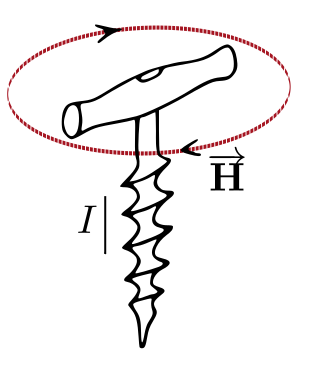
\includegraphics[width=0.3\linewidth]{pravidlo_pravotociveho_sroubu.pdf}}
           \caption[Pravidlo pravé ruku a pravotočivého šroubu]{Určení směru vektoru $\vr{H}$: a)
                   pravidlem pravé ruky; b) pravidlem pravotočivého šroubu}
           \label{temp:fig_urceni_H}
         \end{figure}
    K procvičení těchto pravidel je na obr. \ref{TEMP:fig_ind_c_kruh_z} vyznačen směr indukčních
    čar kruhové\-ho závitu. Označení $\bigotimes$ vyjadřuje proud vstupující  do nákresny (symbol
    letícího šípu od pozorovatele) a označením $\bigodot$ proud vystupující z nákresny (symbol
    hrotu šípu).
    
    \begin{figure}[ht!]
      \centering
      \includegraphics[width=0.4\linewidth]{mag_ind_cary_kruh_z.pdf}
      \caption{Indukční čáry kruhového závitu.}
      \label{TEMP:fig_ind_c_kruh_z}
    \end{figure}    
    Rovnice \ref{TEMP:eq_zak_celk_I} představuje \textbf{zákon celkového proudu} vyjadřující,
    rovnost oběhového magnetické napětí na libovolné uzavřené orientované křivce $c$ proudu, který
    je s křivkou $c$ spřažen. ''\emph{Spřaženým proudem}'' rozumíme proud, který prochází 
    libovolnou plochou $S$, jež je ohraničená křivkou $c$, přičemž plocha $S$ je orientována vůči 
    křivce $c$ pravotočivě (obr. \ref{TEMP:fig_1MR_pic}). \cite[s.~55]{Mayer2001}.

      \begin{equation}\label{TEMP:eq_zak_celk_I}
        \oint\vr{H}\cdot d\vr{l} = I   
      \end{equation}    
     
      \begin{figure}[ht!]
         \centering
         \includegraphics[width=0.7\linewidth]{1MR_pic.pdf}
         \caption[Zákon celkového proudu]{K zákonu celkového proudu}
         \label{TEMP:fig_1MR_pic}
      \end{figure}

         \begin{figure}[hb!]
           \centering
           \subfloat[$\oint\vr{H}\cdot d\vr{l} = 0$]{\label{TEMP:fig_mag_sprazeny_proud1}
             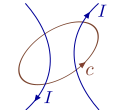
\includegraphics[width=0.3\linewidth]{mag_sprazeny_proud1.pdf}}
           \subfloat[$\oint\vr{H}\cdot d\vr{l} = 0$]{\label{TEMP:fig_mag_sprazeny_proud2}
             \includegraphics[width=0.3\linewidth]{mag_sprazeny_proud2.pdf}}
           \subfloat[$\oint\vr{H}\cdot d\vr{l} = 3I$]{\label{TEMP:fig_mag_sprazeny_proud3}
             \includegraphics[width=0.3\linewidth]{mag_sprazeny_proud3.pdf}}             
           \caption[K pojmu ''proud spřažený s křivkoku'']{K pojmu ''proud spřažený s křivkoku''
                    pro tři různé případy křivky $c$.}
           \label{TEMP:fig_mag_sprazeny_proud123}
         \end{figure}
         
    Základní úlohou řešení stacionárních proudových magnetických polí je určení rozložení veličin 
    $\vr{H}$ a $\vr{B}$ v prostoru, je-li dáno prostorové a materiálové uspořádání a elektrické 
    proudy vybuzují řešené magnetické pole.
    
    V následujících úlohách se omezíme na analýzu jednodušších, souměrných magnetických polí v 
    lineárním izotropním alespoň po částech homogenním prostředí. Pro zjednodušení budeme 
    zanedbávat deformaci magnetického pole v okrajových oblastech a nebudeme uvažovat vliv 
    blízkosti nesymetrického rozhraní a vliv blízkosti druhého zdroje magnetického pole. (Pro 
    přesnější řešení by pak bylo nutné použít tzv. \emph{metodu zrcadlení}.) Některá složitější 
    pole lze rozdělit na několik jednodušších polí souměrného charakteru, resp. typického 
    uspořádání. Vzhledem k tomu, že v předpokládaném lineárním prostředí ($\mu 
    = konst$) platí pro stacionární magnetické pole \emph{princip superpozice}, lze samostatně 
    vyřešit nejprve dílčí jednodušší pole jednotlivých proudů $I_j$ a po jejich superpozici
      \begin{equation}\label{TEMP:eq_superp_mag_pole}
        \vr{H}= \sum_{j=1}^n\vr{H}_j(I_j), \quad\text{resp.}\quad \vr{B}= 
        \sum_{j=1}^n\vr{B}_j(I_j)   
      \end{equation}
    získáme výsledné pole celkového proudu \cite[s.~181]{Kotlan1999}. 
    
    Metodou přímé aplikace I. Maxwellovy rovnice v integrálním tvaru pro stacionární magnetické
    pole proudové
      \begin{equation}\label{TEMP:eq_1MR_rozbor}
        \oint_\mathcal{C}\vr{H}d\vr{l} = \oint_\mathcal{C}H\cos\alpha dl = I_c
      \end{equation}    
    lze jednoduše použít tehdy, je-li ze zadané úlohy zřejmá taková symetrie pole, že lze z 
    nekonečně mnoha uzavřených křivek, splňující rov. \ref{TEMP:eq_1MR_rozbor}, nalézt takovou 
    integrační dráhu $c$, která obepíná proud $I_c$ vytvářející magnetické pole a v jejichž bodech 
    platí podmínka
      \begin{equation}\label{TEMP:eq_H_alpha_konst}
        H = \text{konst}, \qquad \alpha = \text{konst},
      \end{equation}    
    speciálně
      \begin{equation}\label{TEMP:eq_alpha_0}
        H = \text{konst}, \qquad \alpha = 0.
      \end{equation}
    
    Podmínka $\alpha = 0$, tj. $\vr{H}\| d\vr{l}$ je identicky splněna na siločáře magnetického 
    pole. Siločáry souměrných stacionárních magnetických polí splňují tedy podmínku 
    \ref{TEMP:eq_alpha_0} a řešení rovnice \ref{TEMP:eq_1MR_rozbor} při integraci po takovéto 
    siločáře je jednoduché
      \begin{equation}\label{TEMP:eq_1MR_alpha0}
        \oint_\mathcal{C}\vr{H}d\vr{l} = H\underbrace{\oint_\mathcal{C} dl}_{l_c} = 
                                         I_c \rightarrow H = \frac{I_c}{l_c}
      \end{equation}            
    kde $l_c$ je délka integrační dráhy $c$ splňující podmínku \ref{TEMP:eq_alpha_0}.
      
    Klasickým případem takovéto úlohy je magnetické pole \emph{dlouhého přímého válcového vodiče} o
    poloměru $a$, délky $l$ protékaného proudem $I$ rozloženým po průřezu souměrně kolem osy 
    vodiče, tzn, obecně s hustotou $J = J(r)$. Z osové (rotační) symetrie vyplývá, že siločáry 
    magnetického pole mají tvar soustředných kružnic se středem v ose vodiče, ležících v rovině 
    kolmé na osu vodiče obr. \ref{TEMP:fig_mag_pole_vodic_I_konst}.
    \begin{figure}[ht!]
      \centering
      \includegraphics[width=0.7\linewidth]{mag_pole_vodic_I_konst.pdf}
      \caption[Pole dlouhého dutého vodiče protékaného konstantním proudem]{Pole dlouhého dutého
               vodiče protékaného konstantním proudem}
      \label{TEMP:fig_mag_pole_vodic_I_konst}
    \end{figure}        
    Úlohy proto řešíme ve válcových souřadnicích s osou $z$ totožnou s osou vodiče. Za 
    předpokladu, že průměr vodiče je zanedbatelný vůči jeho délce lze zanedbat deformaci pole 
    vlivem konců válcového vodiče a přejít na rovinný problém v polárních souřadnicích. Z důvodu 
    osové  souměrnosti je však pole závislé jen na vzdálenosti $r$ od osy vodiče tj. $$H = H(r), 
    \qquad B = B(r).$$ Na kruhových siločárách je tedy splněna podmínka \ref{TEMP:eq_alpha_0} a z 
    I. Maxwellovy rovnice \ref{TEMP:eq_1MR_rozbor} 
      \begin{equation}\label{TEMP:eq_1MR_rozbor2}
        \oint_{\mathcal{C}}\vr{H}d\vr{l} = H\cos0\oint_\mathcal{C}dl = I(r),
      \end{equation}     
    kde $c$ je kružnice o poloměru $r$ a proud $I(r)$ je dán rovnicí
      \begin{equation}\label{TEMP:eq_1MR_Ir}
        I(r) = \int_{S(r)}\vr{J}(r)d\vr{S} = \int_0^rJ(r)2\pi rdr
      \end{equation}           
    je proud protékající přes kruhovou plochu $S(r)$ ohraničenou kružnicí o poloměru $r$. Pak
    intenzita magnetického pole ve vzdálenosti $r$ od osy vodiče má velikost
      \begin{equation}\label{TEMP:eq_Hr_vodice}
        H = H(r) = \frac{I(r)}{2\pi r},
      \end{equation}       
    a magnetická indukce 
      \begin{equation}\label{TEMP:eq_Br_vodice}
        B = B(r) = \frac{\mu I(r)}{2\pi r},
      \end{equation}       
    přičemž $\mu$ je \emph{permeabilita} v bodech na poloměru $r$. Magnetické pole v okolí
    kruhové\-ho přímého vodiče protékaného proudem $I$ viz obr. \ref{teo:fig021} je tedy v souladu 
    s předchozími úvahami dáno výrazy \cite[s.~183 - 185]{Kotlan1999}:
    \begin{figure}[ht!]
      \centering
      \includegraphics[width=0.8\linewidth]{teo_fig021.pdf}
      \caption[Průběh intenzity magnetického pole dlouhého dutého vodiče protékaného konstantním
               proudem]{Průběh intenzity magnetického pole dlouhého dutého vodiče protékaného
               konstantním proudem}
      \label{teo:fig021}
    \end{figure}      
      \begin{equation}\label{TEMP:eq_Hr_Br_vodice}
        H = H(r) = \frac{I}{2\pi r}, \qquad B = B(r) = \frac{\mu I}{2\pi r}.
      \end{equation}   
    Jelikož 1. MR má nenulovou pravou stranu v magnetickém poli obecně není splněna nutná a
    postačující podmínka, aby magnetické napětí
      \begin{equation}\label{TEMP:eq_mag_napeti}
        \int_{M(l)}^N\vr{H}d\vr{l} = U_{m_{MN}} \qquad [A]
      \end{equation}       
    nezáviselo na tvaru integrační cesty $l$ z $M$ do $N$. Tedy obecně nelze zavést \emph{skalární
    magnetický potenciál}. Magnetické pole je tedy obecně \textbf{vírové (nepotenciální)}.

    Všimněme si však speciálních případů, kdy pravá strana 1. MR je nulová a tedy magnetické pole
    bude \textbf{nevírové (magnetostatické)}. K tomu dochází buď v oblasti kde 
      \begin{equation}\label{TEMP:eq_1MR_0}
        \oint_{\mathcal{C}}\vr{H}d\vr{l} = 0
      \end{equation}    
    tj. takové v němž neexistuje uzavřená křivka $c$ spřažená s nějakým proudem, nebo v takovém
    bodu, v němž platí
      \begin{equation}\label{TEMP:eq_rotH_0}
        \rot{\vr{H}} = 0
      \end{equation}
    tj. v bodu v němž je $\vr{J} = 0$.
    
    Analogicky jako v elektrostatice, lze pak zavést magnetický potenciál $\varphi_m$ vztahem  
      \begin{equation}\label{TEMP:eq_grad_varphi_m}
        \vr{H} = - \grad{\varphi_m}.
      \end{equation}              
    Jednotkou $\varphi_m$ je \emph{ampér} [A]. Pro magnetické napětí mezi body $M, N$ platí
    analogicky
      \begin{equation}\label{TEMP:eq_Umn_def}
        U_{MN} = \int_{M(l)}^N\vr{H}d\vr{l} = \varphi_m(M) - \varphi_m(N),
      \end{equation}        
    nezávisle na integrační cestě $l$. 
     
    % ----------------Magnetické pole vodičů s proudem v homogenním izotropním prostředí ----------
    \subsection{Magnetické pole vodičů s proudem v homogen\-ním izo\-trop\-ním prostředí}
      Z předchozí kapitoly vyplývá, že intenzitu magnetického pole $\vr{H}$ lze stanovit pomocí
      vztahu $\oint\vr{H}\cdot d\vr{l} = I$ tehdy, víme-li předem, že daným bodem prochází silová
      čára, na níž je intenzita pole konstantní, $H_s = \text{konst}$. V tomto případě se křikový
      integrál změní v pouhý součin intenzity pole a délky silové čáry
       
       \begin{equation}\label{TEMP:eq_1MR_v_hom_p}
         \oint_\mathcal{C}\vr{H}d\vr{l} = H_s\oint_\mathcal{C}\vr{l} = H_s\cdot l_s
       \end{equation}      
       
      takže lze vypočítat intenzitu pole $$H_s = \frac{I}{l_s}$$ pro body silové čary. 
      
      Tohoto postupu lze použít i tam, kde uvedená podmínka není splněna, avšak pole lze vyjádřit
      superpozicí dílčích polí, z nich každé tuto podmínku splňuje, viz příklad 
      \ref{TEMP:ex_koax_H}. 

      % --------example: $H=f(r)$ dlouhého dutého válcového vodiče ------
      % \label{TEO:exam012}
      % !TeX spellcheck = cs_CZ
\begin{example}
  Stanovte intenzitu magnetického pole $H=f(r)$ dlouhého dutého válcového vodiče podle obr.
  \ref{TEMP:fig_pole_duty_valec} při rovnoměrném rozložení proudu $I$ po průřezu. 
  
   {\centering
    \captionsetup{type=figure}
    \includegraphics[width=0.6\linewidth]{duf_duty_valec_H.pdf}
    \captionof{figure}{K příkladu stanovení intenzity magnetického pole dlouhého dutého válcového 
               vodiče protékaného proudem}
    \label{TEMP:fig_pole_duty_valec}
  \par}
  
  Vodič s rovnoměrně rozloženým proudem podle obr. \ref{TEMP:fig_pole_duty_valec} je rotačně
  souměrný podle své osy a tedy i jeho magnetické pole je souměrné. Silové čáry jsou soustředné
  kružnice, vektor $\vr{H}$, jenž má směr tečny ke kružnici, je po celé délce kružnice stejně
  velký. Lze tedy snadno použít integrálního tvaru 1. MR (\textbf{zákon celkového proudu})
  
  Pro body ležící vně vodiče obepíná kruhová integrační dráha (vedená po silové čáře 1) celý
  proud vodiče $I$ a platí
  \begin{equation}\label{TEMP:eq_1MR_duty_valec}
    \oint_\mathcal{C}\vr{H}d\vr{l} = H\cdot 2\pi r = I
  \end{equation}
  takže intenzita pole je
  \begin{equation}\label{TEMP:eq_H_duty_valec}
    H = \frac{I}{2\pi r}
  \end{equation}
  
  Ve stěně dutého magnetického vodiče jsou silové čáry rovněž kružnice, neboť magnetické pole
  je i zde souměrné. Tyto siločáry však obepínají jen část proudu $I'$ vodiče pro oběh siločáry
  2 platí
  \begin{equation}\label{TEMP:eq_1MR_uvnitr_valce}
    \oint_\mathcal{C}\vr{H}d\vr{l} = H\cdot 2\pi r = I' = \pi(r^2-r_1^2)J
  \end{equation}
  kde $J$ je hustota proudu ve vodiči
  \begin{equation}\label{TEMP:eq_J_duty_valec}
    J = \frac{I}{S}= \frac{I}{\pi(r_2^2-r_1^2)}
  \end{equation}
  Ve stěně vodiče je tedy intenzita pole
  \begin{equation}\label{TEMP:eq_H_uvnitr_valce}
    H = \frac{I}{2\pi r}\frac{r^2-r_1^2}{r_2^2-r_1^2}
  \end{equation}
  V dutině vodiče je intenzita rovna nule. Vzhledem k souměrnosti pole by i zde muselo platit
  $\oint_\mathcal{C}\vr{H}d\vr{l} = H\cdot 2\pi r$. Protože dráha s poloměrem $r<r_1$ neobepíná
  žádný proud, je $\oint_\mathcal{C}\vr{H}d\vr{l} = 0$ a tedy musí byt $H = 0$.
\end{example}    
  
      %------------------------------------------------------------------

      % --------example: $H=f(r)$ souosého kabelu -----------------------
      % \label{TEO:exam013}
      % !TeX spellcheck = cs_CZ
\begin{mdframed}[style=mdexam]
  \begin{example}\label{TEMP:ex_koax_H}
    Stanovte intenzitu magnetického pole dlouhého přímého souosého kabelu podle obr.
    \ref{teo:fig066}. Středním vodičem (\emph{žílou}) prochází proud $I$ a týž proud
    opačného smyslu prochází vnějším vodičem (\emph{pláštěm}). Proudy jsou rovnoměrně rozloženy po
    průřezech vodičů. Nakreslete graf průběhu $H = f(r)$ \cite[s.~92]{Dufek1970},
    \cite[s.~195]{Kotlan1999}.
    
    {\centering
    \luafigure[0.45]{teo_fig066a.pdf}     \hspace{1em}
    \luafigure[0.45]{teo_fig066b.pdf}
    \captionsetup{type=figure}  
    \captionof{figure}{K příkladu stanovení intenzity magnetického pole dlouhého souosého kabelu
      protékaného proudem: a) náčrt; b) $H=f(r)$}           
    \label{teo:fig066}
    \par}
 
    \textbf{Řešení}: \newline Rovnici \ref{TEMP:eq_1MR_v_hom_p} aplikujeme na jednotlivé intervaly
    osově souměrného stacionárního magnetického pole, přičemž se prakticky jedná o superpozici dvou
    polí. V oblasti $r<r_2$ se uplatňuje pouze pole vnitřního válcového vodiče (žíly), pro $r>r_2$
    přistupuje souosé pole vnějšího trubkového vodiče.
    \begin{itemize}
      \item Pro oblast $r<r_1$ je vzhledem k 
            \begin{align*}
                % \nonumber to remove numbering (before each equation)
                \dd{I}&= \vr{J}d\vr{S} \\
                I(r)  &= \int_S dI = \int_S \vr{J}d\vr{S} = \int_S J\cos\beta dS \\
                      &= \left\lvert\begin{array}{cc}
                                \beta = 0 & H = \text{konst}   \\
                              S = \pi r^2 & dS = 2\pi r\dd{r}  \\
                              \end{array}
                        \right\rvert                                           \\
                      &= J\int_0^r 2\pi rdr = J\pi r^2
            \end{align*}
            hledané řešení 1. MR dáno 
            $$\oint_{\mathcal{c}}\vr{H}d\vr{l} = H_1 2\pi r = I(r) = J\pi r^2$$ kde celková proudová
            hustota je  $$J = \frac{I}{\pi r_1^2}$$ a tedy
            $$H_1 = \frac{I}{2\pi r_1^2}\cdot r$$
            
      \item Pro oblast $r_2>r>r_1$ řešíme v podstatě pole vně osamoceného válcového vodiče $I(r)$ a
            tedy $$H_2 = \frac{I}{2\pi r}$$
      \item Pro $r>r_3$ je magnetické pole vytvářeno celým proudem žíly $I$ a příslušnou částí
            proudu pláště $J\pi(r^2 - r_2^2)$, kde proudová hustota $$J =
            \frac{I}{\pi(r_3^2-r_2^2)}$$ má opačnou orientaci oproti proudové hustotě žíly. Pak 
            \begin{align*}
              I(r)                             &= I - I\frac{r^2-r_2^2}{r_3^2-r_2^2} \\
              \oint_{\mathcal{c}}\vr{H}d\vr{l} &= H_32\pi r = I(r)                   \\          
              H_3                              &= \frac{I}{2\pi r}\left(1 - 
              \frac{r^2 - r_2^2}{r_3^2 - r_2^2}\right) 
            \end{align*}
            Stejný výsledek dostaneme superpozicí opačně orientovaných polí
            $$H_3 = H'_3 - H''_3 = \frac{I}{2\pi r} - \frac{I}{2\pi r}\left(\frac{r^2 - r_2^2}{r_3^2
            - r_2^2}\right)$$. 
    \end{itemize}
    Průběh $H(r)$ je na obr. \ref{teo:fig066}.
  \end{example}
\end{mdframed}  
      %------------------------------------------------------------------

    % -----------Magnetické pole elektrického proudu v diferenciálním tvaru-----------------------
    \subsection{Magnetické pole elektrického proudu v diferenciálním tvaru}
      Nechť je opět magnetické pole vyvoláno konstantním el. proudem $I = \text{konst}$. Jak
      vyplývá z předchozí kapitoly, základním vztahem pro toto pole je \emph{Ampérův zákon}
      $$\oint_\mathcal{c}\vr{H_c}d\vr{l} = I$$  Zvolme za integrační dráhu $c$ obvod malé plošky
      $\Delta S$, jíž prochází proud $\Delta I = J_n \Delta S$, kde $J_n$ je průmět vektoru hustoty
      proudu do směru normály plošky $\Delta S$ (předpokládáme, že ploška $\Delta S$ je dostatečně
      malá, aby se dalo počítat s konstantní hustotou proudu v celém jejím rozsahu)
      \cite[s.~13]{Trnka1972}. Pro zvolený případ platí
      
      \begin{equation}\label{TEMP:eq_amp_z1}
        \oint_\mathcal{c}\vr{H_c}d\vr{l}  =
           J_n \Delta S \rightarrow \frac{1}{\Delta S}\oint_\mathcal{c}\vr{H_c}d\vr{l} = J_n
      \end{equation} 
      
      Pro $\Delta S \rightarrow 0$ zavedeme označení 
      \begin{equation}\label{TEMP:eq_amp_z2}
        \rot{H}  = \frac{1}{\Delta S}\oint_\mathcal{c}\vr{H_c}d\vr{l}  = J_n
      \end{equation}
      
      Rovnice \ref{TEMP:eq_amp_z2} říká, že \emph{rotace vektoru} $\vr{H}$, ($\rot{H}$), jehož
      průmět do určitého směru je roven průmětu vektoru hustoty proudu do tohoto směřu. Z uvedených
      vztahu je patrný fyzikální význam rotace vektoru $\vr{H}$. Je to vektor, jehož velikost je
      rovna oběhovému magnetickému napětí po dráze v rovině kolmé k vektoru hustoty proudu,
      vztaženém k ploše obepínané oběhovou drahou (v nehomogenní poli to platí pro případ, že se
      plocha dráhy blíží k nule).
      
      Při použití pravoúhlé soustavy kartézských souřadnic $x$, $y$ a $z$ jsou průměty vektoru
      $\rot{H}$ do jednotlivých os
      \begin{equation}\label{TEMP:eq_amp_z3}
        \textsf{rot}_x\mathbf{H} = J_x, \qquad 
        \textsf{rot}_y\mathbf{H} = J_y, \qquad
        \textsf{rot}_z\mathbf{H} = J_z
      \end{equation}      
      Průmět $\textsf{rot}_x\mathbf{H}$ je dán oběhovým magnetickým napětím po obvodu plošky $dydz$
      a platí
      \begin{align}\label{TEMP:eq_amp_z4}
        \textsf{rot}_x\mathbf{H} 
          &= \frac{1}{dydz}\oint_\mathcal{c}\vr{H_c}d\vr{l}                   \nonumber \\
          &= \frac{1}{dydz}\left[H_ydy + 
                           \left(H_z + \pder{Hz}{y}dy\right)dz\right] -       \nonumber \\
          &- \frac{1}{dydz}\left[\left(H_y - 
                           \pder{Hy}{z}dz\right)dy - H_zdz\right]             \nonumber \\
          &= \frac{1}{dydz}\left[\pder{Hz}{y}dydz - \pder{Hy}{z}dydz\right]   \nonumber \\
          &= \pder{Hz}{y} - \pder{Hy}{z} = J_z
      \end{align}       
      
      \begin{figure}[ht!]
        \centering
        \includegraphics[width=0.65\linewidth]{rotH_dxdy.pdf}
        \caption[K odvození pojmu $\textsf{rot}_z\mathbf{H}$]{K odvození pojmu
                 $\textsf{rot}_z\mathbf{H}$}
        \label{TEMP:fig_rotH_dxdy}
      \end{figure}            
      tedy dostáváme
      \begin{align}\label{TEMP:eq_amp_z5}
        \textsf{rot}_x\mathbf{H} &= \pder{H_z}{y} - \pder{H_y}{z} = J_x       \nonumber \\
        \textsf{rot}_x\mathbf{H} &= \pder{H_x}{z} - \pder{H_z}{x} = J_y       \nonumber \\
        \textsf{rot}_x\mathbf{H} &= \pder{H_y}{x} - \pder{H_x}{y} = J_z            
      \end{align}        
      Pro \emph{pravoúhlé souřadnice} $x, y, z$ můžeme tedy vztah $\rot{H} = \vr{J}$ rozepsat na
      tvar
      \begin{equation*} % \label{TEMP:eq_amp_z6}
        \textsf{rot}\mathbf{H} 
           = \vr{i}\,\textsf{rot}_x\mathbf{H} + 
             \vr{j}\,\textsf{rot}_y\mathbf{H} +
             \vr{k}\,\textsf{rot}_z\mathbf{H}
     \end{equation*}
     \begin{align*}
         \.&= \vr{i}\left(\pder{H_z}{y} - \pder{H_y}{z}\right) +  
             \vr{j}\left(\pder{H_x}{z} - \pder{H_z}{x}\right) +
             \vr{k}\left(\pder{H_y}{x} - \pder{H_x}{y}\right)                 \\  
         \.&= \vr{i}\,J_x + \vr{j}\,J_y + \vr{k}\,J_z = \vr{J}.
      \end{align*}          
      
      Rotaci vektoru $\rot{H}$ můžeme též symbolicky vyjádřit vektorovým součinem Hamiltonova
      operátoru a vektoru $\vr{H}$
      \begin{align*} %\label{TEMP:eq_amp_z7}
        \rot{H}  &= \nabla\times\vr{H}                                                      \\
                 &= \left(\vr{i}\,\pder{ }{x} + 
                   \vr{j}\,\pder{ }{y} + \vr{k}\,\pder{ }{z}\right)\times(\vr{i}\,H_x +
                   \vr{j}\,H_y + \vr{k}\,H_z)
      \end{align*}
      nebo také determinantu
      \begin{equation}\label{TEMP:eq_amp_z8}
        \rot{H} = \begin{vmatrix}
                    \vr{i}       & \vr{j}      & \vr{k}      \\
                    \pder{ }{x}  & \pder{ }{y} & \pder{ }{z} \\ 
                    H_x          & H_y         & H_z         \\
                  \end{vmatrix}      
      \end{equation}  
      \emph{cylindrických souřadnic} $r$, $\varphi$, $z$:
      \begin{align}\label{TEMP:eq_amp_z9}
        \textsf{rot}_r\mathbf{H}       
          &= \frac{1}{r}\pder{H_z}{\varphi} - \pder{H_\varphi}{z} = J_r           \nonumber \\ 
        \textsf{rot}_\varphi\mathbf{H} 
          &= \pder{H_r}{z} - \pder{H_z}{r}                        = J_\varphi     \nonumber \\
        \textsf{rot}_z\mathbf{H}       
          &= \frac{1}{r}\left[\pder{ }{r}
             \left(rH_\varphi\right)-\pder{H_r}{\varphi}\right]   = J_z
      \end{align} 
      \emph{sférických souřadnic} $r$, $\varphi$, $\vartheta$ 
      \begin{align}\label{TEMP:eq_amp_z10}
        \textsf{rot}_r\mathbf{H}        
           &= \frac{1}{r\sin\vartheta}\left[\pder{ }{\vartheta}(H_\varphi\sin\vartheta) - 
              \pder{H_\vartheta}{\varphi}\right]                     = J_r           \nonumber \\ 
        \textsf{rot}_\varphi\mathbf{H}   
           &= \frac{1}{r}\left[\pder{ }{r}(rH_\vartheta) - 
              \pder{H_r}{\vartheta}\right]                           = J_\varphi     \nonumber \\
        \textsf{rot}_\vartheta\mathbf{H} 
           &= \frac{1}{r\sin\vartheta}\left[\pder{H_r}{\varphi} -
              \pder{ }{r}\left(rH_\varphi\sin\vartheta\right)\right] = J_\vartheta    
    \end{align} 
      Podobně jako v elektrickém poli vyjadřujeme vztah $\oint\vr{D}d\vr{S} = Q$ vztahem $\diver{D}
      = \rho$, tak i v magnetickém poli vyjadřujeme vztah $\oint\vr{B}d\vr{S} = 0$ vztahem
      $\diver{D} = 0$, nebo též v kartézských souřadnicích $x$, $y$ a $z$ jako $$\diver{D} =
      \nabla\cdot\vr{B} = \pder{B_x}{x} + \pder{B_y}{y} + \pder{B_z}{z} = 0$$
                     
    % ----------------Rovnice pro magnetický potenciál -------------------------------------------
    \subsection{Rovnice pro magnetický potenciál}
      V regulárních bodech lineárního homogenního izotropního magnetika platí pro $\varphi_m$
      \textbf{Laplaceova rovnice}
      \begin{equation}\label{TEMP:eq_varphi_m_laplace}
        \Delta\varphi_m = 0
      \end{equation}      
      Důkaz plyne z rovnice $\diver{B} = 0$ a rovnice $\vec{B} = \mu\vec{H}$: $$\diver{B} =
      \textsf{div}\mu\vec{H} = \textsf{div}\mu(-\textsf{grad}\varphi_m).$$ Pro $\mu = \text{konst}$
      dostáváme $\textsf{div}\textsf{grad}\varphi_m = 0$, což je rovnice
      \ref{TEMP:eq_varphi_m_laplace}.
      
      Na rozhraní mezi dvěma magneticky různými prostředími neplatí Maxwellovy rovnice v
      diferenciálním tvaru a tedy ani Laplaceova rovnice \ref{TEMP:eq_varphi_m_laplace}. Podmínky 
      pro $\vr{H}$ a $\vr{B}$ na rozhraní vyjádříme pomocí skalárního magnetického potenciálu
       \begin{align}\label{TEMP:eq_mag_U_rozhrani}
         \varphi_{m1}                 &= \varphi_{m2} \\
         \mu_1\pder{\varphi_{m1}}{n}  &= \mu_2\pder{\varphi_{m2}}{n} 
       \end{align}
      kde $\pder{}{n}$ jsou derivace ve směru normály k rozhraní. 
    
    \subsubsection{Vektorový magnetický potenciál}
      V elektrostatice jsme pro usnadnění mnohých problémů zavedli skalární elektrický potenciál -
      lze jej zavést vždy, neboť elektrostatické pole je vždy potenciální. Magnetické pole je však
      obecně vírové. Lze jej popsat skalárním potenciálem jen ve speciálních případech, tj.
      jestliže je polem potenciálním. Obecně je však zavedení skalárního potenciálu nepřípustné.
      Lze i pak zavést nějakou veličinu (analogickou skalárnímu potenciálu), s níž by se pracovalo
      snáze, než přímo s vektory pole?
      
      Dříve než definujeme vektorový magnetický potenciál, zopakujme zavedení skalárního potenciálu
      v elektrostatice. Vyjdeme z 2. MR a z rovnice známé z vektorové analýzy: $$\rot{E} = 0 \qquad
      \text{a} \qquad \textsf{rot}\,\textsf{grad}\varphi_m = 0.$$
      
      V magnetickém poli vyjdeme ze 4. MR a z jiné identity pro vektorovou funkci $\vr{A}$, známe z
      vektorové analýzy: $$\diver{B} = 0 \qquad \text{a} \qquad \textsf{div}\textsf{rot}\vec{A} =
      0$$ odtud
        \begin{equation}\label{TEMP:eq_B_rotA}
          \vec{B} = \rot{A}.
        \end{equation}       
               
%} % tikzset
%~~~~~~~~~~~~~~~~~~~~~~~~~~~~~~~~~~~~~~~~~~~~~~~~~~~~~~~~~~~~~~~~~~~~~~~~~~~~~~~~~~~~~~~~~~~~~~~~~~
\printbibliography[title={Seznam literatury}, heading=subbibliography]
\addcontentsline{toc}{section}{Seznam literatury}
  \input{../src/TEO/chap/magn1ch01.tex} 
}{ % DEBUG was off
\LuaPartBckgrnd{titleBG_fractal1.png}
\LuaPartTitle{MAGN}{Magnetické obvody}{MAGN}
\parttoc
%========== Kapitola: Spojité matematické modely jednotlivých polí =================================
  % !TeX spellcheck = cs_CZ
%file:spojity_model_elmag_p.tex
%{\tikzset{external/prefix={tikz/TEO/}}
% \tikzset{external/figure name/.add={ch01_}{}}
%==============================Kapitola: Spojité matematické modely jednotlivých polí ==============
\chapter{Spojité matematické modely polí}
\minitoc
  \section{Elektromagnetické pole}       
    \subsection{Veličiny elektromagnetického pole a jejich jednotky}
      \fbox{Elektrický náboj} je \emph{skalární veličinou}. Jednotkou je \emph{coulomb [C]}. Má
         kvantový charakter (tj. je roven celistvému násobku elementárního náboje $e =
         1,602\cdot10^{-19}C$), avšak v technických aplikacích k tomu nepřihlížíme. Náboj $Q$
         může být rozložen:
         \begin{itemize}\addtolength{\itemsep}{-0.5\baselineskip}
            \item \emph{prostorově} v objemu $V$ s objemovou hustotou
               \begin{equation}\label{TEMP:eq_q_varrho}
                  \varrho = \frac{dQ}{dV} \qquad [C\cdot m^{-3}]
               \end{equation}               
            \item \emph{plošně} na ploše $S$, s plošnou hustotou
               \begin{equation}\label{TEMP:eq_q_sigma}
                  \sigma = \frac{dQ}{dS} \qquad [C\cdot m^{-2}]
               \end{equation}                 
            \item \emph{lineárně} na křivce $l$, s lineární hustotou
               \begin{equation}\label{TEMP:eq_q_tau}
                  \tau = \frac{dQ}{dl} \qquad [C\cdot m^{-1}]
               \end{equation}                 
         \end{itemize}
         Rozlišujeme:
           \begin{itemize}\addtolength{\itemsep}{-0.5\baselineskip}
             \item \textbf{volné náboje}: mohou se přemisťovat v makroskopických
             vzdálenostech,
             \item \textbf{vázané náboje}: mohou se přemisťovat jen v
             mikroskopických vzdálenostech.
           \end{itemize}
         Volnými náboji jsou volné elektrony v kovech nebo ionty v elektrolytech (jsou odpoutány od
         atomů, resp. molekul a volně se mezi nimi pohybují); vázané náboje vznikají polarizací
         dielektrika.
         
      \vspace{1em}
      \fbox{Elektrický proud}\label{TEMP:kap_el_proud_velicina} je znám z každodenního života,
        přesto je velmi důležité umět tento pojem vnímat jak pro označení „jevu“ (kap.
        \ref{TEMP:kap_elproud_jev}), tak jako fyzikální veličinu, která tento jev kvantitativně
        popisuje (kap. \ref{TEMP:kap_el_proud_velicina} ). Elektrický proud je \emph{skalární
        fyzikální veličina} tzn. $I$ resp. $i$, jejíž jednotkou je základní jednotka soustavy SI:
        \emph{ampér} – [A]. V této soustavě jednotek je ampér definován na základě silových
        účinků mezi dvěma vodiči, kterými prochází elektrický proud. Tato síla je magnetického
        původu, avšak magnetické pole vzniká jako důsledek pohybu elektrického náboje.Je tvořen
        uspořádaným pohybem elektrických nábojů.
        
        Připojíme-li vodič ke zdroji elektrického napětí, elektrické pole uvnitř působí elektrickou
        silou na vodivostní elektrony, vyvolává jejich pohyb a tím vytváří elektrický proud, který
        je po krátké době \emph{stacionární} (ustálený, nezávislý na čase). Jestliže vodičem projde
        náboj $\Delta Q$ resp. $dQ$ za časový interval $\Delta t$ resp. $dt$, lze definovat
        \emph{průměrný} resp. \emph{okamžitý} proud ve vodiči:
        \begin{itemize}\addtolength{\itemsep}{-0.5\baselineskip}
          \item \textbf{průměrný} elektrický proud: $$I_{AV} = \frac{\Delta Q}{\Delta t}
                \qquad[A],$$
          \item \textbf{okamžitý} elektrický proud (který je limitním případem proudu průměrného,
                studujeme-li množství náboje, které projde průřezem vodiče za infinitezimální
                (nekonečně krátký) časový interval): $$i = \lim_{\Delta t \rightarrow 0}\frac{\Delta
                Q}{\Delta t} = \frac{dQ}{dt} \qquad[A].$$ V ustáleném stavu protéká všemi průřezy
                vodiče stejně velký proud,
          \item speciálně pohybuje-li se náboj vodičem rovnoměrně, nazýváme proud
                \textbf{stejno\-směr\-ným}, $I(t) = \text{konst}$, a platí $$ I_{DC} =
                \frac{Q}{t}\qquad[A] $$
        \end{itemize}        

        Elektrický proud jako \emph{jev} charakterizuje jednu z forem fyzikálního pohybu, kterou je
        \textbf{uspořádaný pohyb elektricky nabitých částic} v látce. Přestože jakýkoliv elektrický
        proud je vždy tvořen pohybujícími se náboji, nemusí všechny pohybující se náboje vytvářet
        elektrický proud. Ve vodiči dochází ke vzniku trvalého elektrického proudu za těchto
        podmínek:
          \begin{itemize}\addtolength{\itemsep}{-0.5\baselineskip}
            \item vodič se musí nacházet v trvalém elektrickém poli, což je realizováno pomocí tzv.
                  \emph{zdroje} (generátoru) elektrického napětí,
            \item ve vodiči musí být přítomny volné nosiče elektrického náboje.
          \end{itemize}
        
        Podle charakteru vnějšího elektrického pole lze rozlišit tři základní druhy proudů:
          \begin{labeling}{stejnosměrný}\addtolength{\itemsep}{-0.5\baselineskip}
            \item[\textbf{stejnosměrný}] proud vzniká tehdy, jestliže má intenzita elektrického pole
                   konstantní orientaci,
            \item[\textbf{střídavý}] proud ve vodiči vytváří vnější elektrické pole, jehož intenzita
                  periodicky mění svou orientaci na opačnou,
            \item[\textbf{stacionární}] stejnosměrný proud vzniká ve vodiči, je-li intenzita
                  elektrického pole konstantní co do velikosti, směru i orientace.
          \end{labeling}  

       Nabité částice představující volný náboj ve vodičích jsou v neustálém chaotickém tepelném
       pohybu (viz molekulová fyzika a termodynamika). Jedná se o \emph{mikroskopický pohyb}, který
       nemá za následek makroskopicky pozorovatelné přemístění náboje. Pokud ve vodiči vytvoříme
       elektrické pole, tepelný pohyb nabitých částic neustane, ale k náhodné složce rychlosti
       přibude ještě složka rychlosti ve směru vloženého pole.
       
       Při studiu elektrického proudu v kovových vodičích se zabýváme ustálenými proudy
       vodivostních elektronů, které v kovu vytváří tzv. \emph{elektronový plyn}. Tyto vodivostní
       elektrony jsou téměř volné a pohybují se v poli kladných iontů uspořádaných v krystalové
       mřížce.
        
       Experimentálně lze elektromagnetické pole prokázat silovým působením na elektricky nabité
       částice. Celkovou sílu $\vec{F}$ lze rozložit na elektrickou sílu $\vec{F}_e$, nezávislou na
       tom, zda je nabitá částice v klidu nebo v pohybu vůči vztažné soustavě a na magnetickou sílu
       $\vec{F}_m$, působící jen na pohybující se částice. Elektromagnetické pole má tedy dvě
       složky: \textbf{elektrické pole}, působící na náboj silou $\vec{F}_e$ a \textbf{magnetické
       pole}, působící na pohybující se náboj silou $\vec{F}_m$  \cite[s.~13]{Mayer2001}.
      
      \vspace{1em}
      \fbox{Intenzita elektrického pole $\vec{E}$} je vektorovou veličinou charakterizující
        \emph{elektrické pole}.
        Je definována jako 
        \emph{síla působící na nepohybující se jednotkový bodový náboj}:
        \begin{equation}\label{TEMP:eq_E}
          \vec{E} = \frac{\vec{F}_e}{Q} \qquad\left[\frac{V}{m}\right]  
        \end{equation}        
        kde $\vec{F}_e$ je elektrická síla působící na náboj $Q$.
      
      \vspace{1em}
      \fbox{Magnetická indukce $\vec{B}$} je vektorovou veličinou charakterizující \emph{magnetické
        pole}. Je definovována vztahem
        \begin{equation}\label{TEMP:eq_B}
          \vec{F}_m = Q(\vec{v}\times\vec{B}) \qquad[T]  
        \end{equation}        
        kde $\vec{F}_m$ je magnetická síla působící na náboj $Q$ pohybující se rychlostí $\vec{v}$.
        Jednotkou je \emph{tesla} $[T]$.
    
        Síla, jež působí elektromagnetické pole na pohybující se náboj se nazývá \textbf{Lorentzova
        síla}
        \begin{equation}\label{TEMP:eq_Lorentz}
          \vec{F} = \vec{F}_e + \vec{F}_m =Q(\vec{E} + \vec{v}\times\vec{B}) \qquad[N]  
        \end{equation}        

    \subsection{Maxwellovy rovnice}
      Makroskopická teorie elektromagnetického pole v klasickém pojetí vychází ze základních zákonů
      vyjádřených \emph{Maxwellovými rovnicemi (MR)}. Lze je zapsat buď v \textbf{integrálním},
      nebo \textbf{diferenciálním tvaru}. V integrálním tvaru popisují elektromagnetické pole v
      jisté prostorové oblasti $\Omega$, kdežto v diferenciálním tvaru ve vnitřním bodě této
      oblasti. Soustavu vlastních MR představují první čtyři páry rovnic; často se k nim připojuje
      jako další základní rovnice elektromagnetického pole rovnice kontinuity pro vodivý proud.
      Její integrální a diferenciální tvar reprezentují poslední dvě rovnice.
exa
      \begin{align}
        \oint_\mathcal{C}\vr{H} d\vr{l} &= I+\der{\Psi}{t}
                                           \quad \rot{H}=\vr{J}+\pder{\vr{D}}{t}             \\
        \oint_\mathcal{C}\vr{E} d\vr{l} &= -\der{\Phi}{t}
                               \qquad \rot{E}=-\pder{\vr{B}}{t}\\
         \int_\mathcal{S}\vr{D} d\vr{S} &= Q \qquad\quad\;   \diver{D}=\rho_V                \\
         \int_\mathcal{S}\vr{B} d\vr{S} &= 0 \qquad\quad\;\; \diver{B}=0                     \\
         \int_\mathcal{S}\vr{J} d\vr{S} &= -\der{Q}{t} \quad\;\;\;\diver{J}=-\der{\rho_V}{t}
      \end{align}

      Předpokládá se, že \emph{všechny křivky a plochy v integrálním tvaru MR jsou po částech
      hladké a všechny integrované veličiny jsou po částech spojité funkce}. Pak je zaručena
      existence integrálů v těchto rovnicích. V diferenciálním tvaru MR se předpokládají pouze
      \textbf{regulární body} oblastí, což jsou body, v nichž jsou veličiny $\vr{E}$, $\vr{D}$,
      $\vr{B}$ a $\vr{H}$ \emph{spojité a spojitě diferencovatelné funkce}; nejsou jimi tedy např.
      body rozhraní dvou různých prostředí, v elektrickém poli body v nichž jsou umístěny diskrétní
      náboje, v magnetickém poli body proudových vláken atd.

      % --------example: Energie v Kondenzátoru ------------------------
      % \label{TEO:exam019}
      % !TeX spellcheck = cs_CZ
\begin{example}\label{teo:exam019}
  Mějme nabitý deskový kondenzátor \(C\), zobrazený na obr. \ref{teo:fig019a}. Zvětšme jeho
  kapacitu, například tím, že zvětšíme plochu jeho elektrod, nebo připojíme paralelně druhý stejné 
  velikosti, viz obr. \ref{teo:fig019b}. Otázka zní, jak velká enerige bude uložena v 
  elektrostatickém poli obou kondeznátorů? Bude energie po rozdělení náboje mezi oba 
  kondenzátory rovna původní energií nabitého kondenzátoru? Pokud ne, vysvětlete kam se část 
  energie transformovala. 
  
   {\centering
    \captionsetup{type=figure}
    \begin{tabular}{cc}
     \subfloat[ ]{\label{teo:fig019a}
       \includegraphics[width=0.15\linewidth]{teo_fig019a.png}}              &
     \hspace{3em}
     \subfloat[ ]{\label{teo:fig019b}
       \includegraphics[width=0.5\linewidth]{teo_fig019b.png}}
    \end{tabular}
    \captionof{figure}{K příkladu \ref{teo:exam019}: a) Nabitý kondenzátor s rovnoběžnými rovinnými 
    elektrodami; b) Rozložení náboje na obou kondenzátorech velikosti}
    \label{teo:fig019}
  \par}
  
  Je-li dielektrikum kondenzátoru lineární, pak pro energii elektrického pole akumulovanou v 
  nabitém kondenzátoru platí. Podrobněji například v kapitole \ref{fyz:IIchapVsecXIX}.
  \begin{equation}
    W = \frac{1}{2}CU^2 \quad\text{nebo}\quad W = \frac{1}{2}\frac{Q^2}{C} 
    \quad\text{kde}\quad C = \frac{Q}{U}
  \end{equation}
  Předpokládejme ustálený stav po připojení druhého kondenzátoru, jak je znázorněno na obr. 
  \ref{teo:fig019b}. V obvodu nepředpokládáme přítomnost odporu, který by způsobil ztrátu energie, 
  vyzářené v podobě tepla. Kapacita je dvojnásobná a náboj zůstal stejný. Na každém kondenzátoru 
  tedy očekáváme polovinu původního náboje. Sečteme-li energii uloženou v elektrických polích obou 
  kondenzátorů dostaneme
  \begin{align*}
    W^* &= \frac{1}{2}\frac{(\frac{1}{2}Q)^2}{C} + \frac{1}{2}\frac{(\frac{1}{2}Q)^2}{C} 
         = \frac{(\frac{1}{2}Q)^2}{C} =\frac{1}{4}\frac{Q^2}{C}                               \\
        &  \xrightarrow[\scriptscriptstyle{C\rightarrow2C}]{}
           \frac{1}{2}\frac{Q^2}{(2C)} = \frac{1}{2}W 
  \end{align*}
  Kupodivu, polovina energie prostě chybí a jelikož platí zákon zachování energie\footnote{viz 
  partie Fyzika \ref{part:FYZI}, kapitola \ref{fyz:IchapII})}, nezbývá nic jiného než uznat, že 
  elektrický obvod dle \ref{teo:fig019b}, nemodeluje fyzikální problém dost věrně. Tím jsme dospěli 
  k závěru, že je nutné do obvodu dodat rezistor, tak jak je znázorněno na obrázku   
  \ref{teo:fig020}.
  
   {\centering
    \captionsetup{type=figure}
    \includegraphics[width=0.4\linewidth]{teo_fig020.png}
    \captionof{figure}{Rezistor \(R\) představuje ztráty, které nebyly v obvodu na obrázku 
               \ref{teo:fig019b} předpokládány}
    \label{teo:fig020}
  \par}
  
  Abychom mohli určit teplné ztráty na rezistoru dané integrálem \(\int_{0}^{\infty} 
  Ri^2(t)\dd{t}\), nedříve sestavíme jednoduchou diferenciální rovnici prvního řádu aplikací II. 
  Kirchhoffova zákona, ze které odvodíme vzorec pro časovou závislost proudu \(i(t)\). 
  \begin{align*}
    \frac{Q_0 - Q}{C} - Ri(t) - \frac{Q_0}{C}         &= 0 \quad/\der{ }{t}             \\
    \frac{-i(t)}{C} - R\der{i(t)}{t} - \frac{i(t)}{C} &= 0                              \\
                                        \der{i(t)}{t} &= - \frac{2}{RC}i(t) \quad/\int  \\
                                                 i(t) &= I_0e^{-\frac{2}{RC}t}
  \end{align*}
  Nyní můžeme stanovit energii disipované na rezitoru \(R\)
  \begin{align*}
    W   &= \int_{0}^{\infty}Ri^2(t)\dd{t} = RI_0^2\int_{0}^{\infty}e^{-\frac{4}{RC}t}\dd{t}   \\
    \shortintertext{Do integrované funkce dosadíme novou proměnnou \(u = \frac{4}{RC}t\), \(\dd{u} 
                    = \frac{4}{RC}\dd{t}\), \(\dd{t} = \frac{RC}{4}\dd{u}\)}
        &= RI_0^2\int_{0}^{\infty}e^{-u}\frac{RC}{4}\dd{u} 
         = R^2I_0^2\frac{C}{4}\underbrace{\int_{0}^{\infty}e^{-u}\dd{u}}_1  \\
    \shortintertext{Jelikož platí \(I_0 = \frac{U}{R}=\frac{Q}{CR}\) dostaneme po dosazení}
        &= \cancel{R^2}\frac{Q^2}{C^2\cancel{R^2}}\frac{C}{4} = \frac{Q^2}{4C}
         = \frac{1}{2}W
  \end{align*}
  Nyní je vše v pořádku. Druhá polovina energie je disipována na rezistoru a navíc z výsledku 
  vyplývá, že vubec nezávisí na \(R\)!
\end{example}


  
      %-----------------------------------------------------------------
      
  % --------------- Stacionární magnetické pole-----------------------------------------------------
  \section{Stacionární proudové pole}
    V elektrostatice (tj. elektrickém poli nepohybujících se nábojů) neexistuje trvalý elektrický
    proud. Zdroje napětí (galvanické články, termočlánky, dynama aj.) mají tu vlastnost, že na
    jejich záporné svorce je trvale nadbytek elektronů, a na jejich kladné svorce jejich
    nedostatek. Těmito zdroji můžeme ve vodiči trvale udržovat elektrické pole a tedy i tok nosičů
    elektřiny. Jestliže se \emph{náboje pohybují konstantní rychlostí, hovoříme o stacionárním
    elektrickém proudu}. Základní rovnice elektrostatické pole jsou:

    \begin{table}[ht!]
      \setlength\extrarowheight{5pt}
      \centering
      \begin{tabular}{lc|c|}
        \cline{2-3}
        \multicolumn{1}{l|}{} 
          & \textbf{integrální tvar} & \textbf{diferenciální tvar}                    \\[8pt]
        \hline
        \multicolumn{1}{|l|}{2. MR} 
          & \(\bigointsss\vr{E}\cdot d\vr{l} = 0\) & \(\rot{E} = 0\)                  \\[8pt] 
        \cline{1-3}
        \hline
        \multicolumn{1}{|l|}{Zákon kontinuity} 
          & \(\bigointsss\vr{J}\cdot d\vr{S}=0\) & \(\diver{J}=0\)                    \\[8pt]
        \cline{1-3}
        \multicolumn{1}{|l|}{Ohmův zákon}
          & \(I=GU=\dfrac{U}{R}\) & \(\vr{J} = \gamma\vr{E} = \dfrac{1}{\rho}\vr{E}\) \\[8pt]
        \cline{1-3}
      \end{tabular}
      \caption{Základní rovnice stacionárního proudového pole}
    \end{table}
    
    \subsection{Elektrický proud v kovových vodičích}\label{TEMP:kap_elproud_jev}
      V předchozí kapitole \ref{TEMP:kap_el_proud_velicina} bylo o elektrickém proudu pojednáváno
      jako o skalární fyzikální veličině. V této kapitole nás bude zajímat makroskopický pohled na
      „jev“ známý jako \emph{elektrický proud}.
      
      Zopakujme, že elektrickým proudem je míněn uspořádaný pohyb elektrických ná\-bo\-jů, a aby se
      tyto náboje mohly pohybovat, musí být volné - jsou přítomny v látkách, které nazýváme
      \textbf{vodiče}. Vodiče mohou mít nositele náboje jednoho znaménka (elektrony v kovech,
      uhlíku a v polovodičových) anebo obojích znamének (kladné a záporné ionty v elektrolytech,
      ionty a elektrony v ionizovaných plynech). Volné nositele náboje (elektrony, ionty) lze
      rovněž oddělit od těchto látek (vodičů) a vytvořit elektrický proud ve vakuu nebo ve
      zředěných plynech.
      
      Z vodičů mají největší význam \textbf{kovy}, které jsou polykrystalickými látkami s kovovou
      vazbou. Každý mikroskopický monokrystal kovu má pevnou krystalovou mříž sestavenou z kladných
      iontů, mezi nimiž se přetržitě pohybují \emph{volné elektrony} rychlost\-mi, jejichž velikost
      je statisticky proměnná (co do velikosti i směru). Střední hodnota rychlosti (jako vektoru)
      všech elektronů je nulová. Střední hodnota rychlosti určitého elektronu je závislá na teplotě
      vodiče. Elektrony konají tzv. \emph{termický pohyb}. Rychlosti neuspořádaných termických
      pohybů dosahují jen o několik řádů větších hodnot, než kmity iontů v krystalech mřížky.

      \begin{figure}
        \centering
        \includegraphics[width=0.5\linewidth]{vd_e_drift.pdf}
        \caption[Pohyb elektronu ve vodiči.]{Pohyb elektronu ve vodiči. Fyzikálně je $v_d$ 
                 průměrná rychlost nosičů náboje uvnitř vodiče, který je vložen do vnějšího
                 elektrického pole. Ve skutečnosti se ale elektron ve vodiči nepohybuje po přímce,
                 jeho pohyb je chaotický.}
        \label{TEMP:fig_vd_e_drift}
      \end{figure}
      
      Připojíme-li vodič k vnějšímu zdroji elektrického pole (např. ke galvanickému článku), začne
      statisticky převládat uspořádaný pohyb nosičů kladného (záporného) náboje ve směru (proti
      směru) vnějšího pole nad termickým pohybem, což v makroskopickém měřít\-ku pozorujeme jako
      \textbf{makroskopický elektrický proud}. Jsou-li ve vodiči přítomny nosiče náboje obou
      polarit, dojde k pohybu ve vzájemně opačných směrech, přičemž směr toku nosičů kladného
      náboje se historicky ztotožňuje se směrem toku elektrického proudu. U kovových vodičů je tedy
      směr proudu právě opačný, než směr toku elektronů, jenž tento elektrický proud tvoří.
      
      Velikost (intenzitu) proudu posuzujeme podle velikosti náboje obojí polarity, který projde
      určitým průřezem vodiče ve vzájemně opačných směrech za jednotku času. Projde-li průřezem
      vodiče celkově náboj $dQ$ za čas $dt$, bude tok náboje vodičem charakterizovat skalární
      veličina
        \begin{equation}\label{TEMP:eq_I_01}
          I = \frac{dQ}{dt} \qquad[A],  
        \end{equation}        
      která se nazývá \emph{elektrický proud}($1C\cdot s^{-1} = 1A $ čteno \emph{ampér}). Tato
      jednotka patří mezi základní jednotky \texttt{SI} soustavy.
      
      Pro \emph{stacionární} (tj. časově neproměnný - ustálený) proud můžeme obecný výraz
      \ref{TEMP:eq_I_01} nahradit rovnicí
        \begin{equation}\label{TEMP:eq_I_02}
          I = \frac{Q}{t}.  
        \end{equation}       
      Jedná-li se o rovnoměrný pohyb bodového náboje $Q$ po kružnici s periodou $T$, resp. s
      úhlovou rychlostí $\omega$, můžeme vzniklý ustálený proud vyjádřit rovnicí 
        \begin{equation}\label{TEMP:eq_I_03}
          I = \frac{Q}{T} = \frac{\omega Q}{2\pi}.  
        \end{equation}
      
      Bude-li se element náboje $dQ$ pohybovat v lineárním útvaru rychlostí $v = \frac{dQ}{dl}$,
      bude po dosazení do rov.\ref{TEMP:eq_I_01} reprezentovat elektrický proud 
        \begin{equation}\label{TEMP:eq_I_04}
          I = \frac{dQ}{dt} = \frac{dQ}{dl}v = \tau v, 
        \end{equation}      
      kde $\tau$ je \emph{délková hustota} náboje a $v$ je velikost \emph{okamžité rychlosti}
      náboje v uvažovaném místě lineárního útvaru. 

      \begin{figure}[ht!]
         \centering
         \includegraphics[width=0.5\linewidth]{el_proud_ve_vodici.pdf}
         \caption[Náboje, pohybující se vodičem]{Směr elektrického proudu byl implicitně stanoven
                  jako směr pohybu kladných nábojů. Nositeli elektrického náboje uvnitř vodičů jsou
                  ovšem záporně nabité volné elektrony, které se tedy dle  konvence pohybují proti
                  směru elektrického proudu. Elektrický proud může protékat pevnými látkami (kovy,
                  polovodiči), kapalinami (elektrolyty) a ionizovanými plyny. Látky, které nevedou
                  elektrický proud, nazýváme nevodiči, izolanty}
         \label{TEMP:fig_el_proud_ve_vodici}
      \end{figure}
      
      Elektrický proud je veličina, která obecně popisuje prostorový jev. Omezíme se nyní na běžný
      případ vodiče, jako je na obr. \ref{TEMP:fig_el_proud_ve_vodici}, který má volné náboje jen
      jedné polarity (u kovových vodičů jde o elektrony) a označme $\rho_0$ prostorovou hustotu
      volného náboje a $v_d$ velikost usměrněné rychlosti jejich nositelů (elektronů). Pak za čas
      $dt$ projde průřezem o obsahu $S_0$ ($S_0\bot v_d$) náboj $dQ = \rho_0 S_0 v_d dt$.
      Elektrický proud vyjádřený rov.
      \ref{TEMP:eq_I_01} můžeme přepsat do tvaru
        \begin{equation}\label{TEMP:eq_I_05}
          I = \rho_0 S_0 v_d = - e n_0 S_0 v_d, 
        \end{equation}         
      kde $\displaystyle{n_0 = \frac{\rho_0}{-e}}$ je počet nositelů volného náboje (tj. v našem
      případě elektronů, z nichž každý nese náboj $-e$ v jednotkovém objemu vodiče, přičemž pro
      elektrony zřejmě je $\rho_0<0$.

      \begin{wrapfigure}[14]{r}{5cm}
        \centering
        \includegraphics[width=0.9\linewidth]{plocha_S.pdf}
        \caption[Rovinná plocha $S$.]{Rovinná plocha $S = S_0\cos\alpha$}
        \label{TEMP:fig_plocha_S}
      \end{wrapfigure}
      Rovinnou plochou $S$ průřezu můžeme zavést jako vektor $vr{S}$, který má směr daný normálou k
      ploše a pravidlem pravé ruky (ukazují-li prsty pravé ruky směr oběhu po hraniční křivce
      plochy, ukáže palec směr plochy jako vektoru $\vr{S}$). Protože driftová rychlost $v_d$ je
      také vektor, nebudeme obecně uvažovat vektory $\vr{S}, \vr{v_d}$ o stejném směru a rovnici
      \ref{TEMP:eq_I_05} přepíšeme do obecnějšího tvaru      
      
      \begin{equation}\label{TEMP:eq_I_06}
        I = \rho_0 \vr{S_0}\cdot\vr{v}_d = jS\cos\alpha = jS_0, 
      \end{equation}      
      kde $S_0 = S$ pro $\alpha = 0$ (viz obr. \ref{TEMP:fig_plocha_S}) a   
      \begin{equation}\label{TEMP:eq_I_07}
        \vr{j} = \rho_0\vr{v_d}, 
      \end{equation}        
      je proudová hustota. Je to vektor o velikosti 
      \begin{equation}\label{TEMP:eq_I_08}
        j = \frac{I}{S\cos\alpha} = \frac{I}{S_0}  \qquad A\cdot m^{-2}, 
      \end{equation}   
      obecněji
      \begin{equation}\label{TEMP:eq_I_09}
        j = \frac{dI}{dS}, 
      \end{equation}

      a o směru vektoru driftové rychlosti nositelů kladného náboje. Pro případ nositelů volného
      náboje - elektronů má proudová hustota opačný směr než driftová rychlost $v_d$ (obr.
      \ref{TEMP:fig_plocha_S}).
      
      Velikost vektoru $\vr{j}$ má význam plošné hustoty elektrického proudu v uvažovaném místě
      průřezu. Jednotkou je $A\cdot m^{-2}$.
      
      Nebude-li proudová hustota na uvažovaném průřezu konstantní, bude celkový elektrický proud
      procházející průřezem o obsahu $S$ dán integrálem 
        \begin{equation}\label{TEMP:eq_I_10}
          I = \int_S \vr{j}d\vr{S}. 
        \end{equation} 

      % --------example: Driftová rychlost elektroknů ve vodiči --------
      % \label{TEO:exam008}
      % !TeX spellcheck = cs_CZ
%---------- Driftová rychlost elektroknů ve vodiči: 
\begin{mdframed}[style=mdexam]
\begin{example}\label{TEO:exam008} \emph{Driftová rychlost elektronů ve vodiči:} Vodičem z 
jednomocné mědi o
  průřezu $S_0 = \SI{1}{\mm^2}$ prochází elektrický proud $I = \SI{5}{\A}$. Vypočtěte:
  \begin{itemize}[noitemsep, leftmargin=2em]
    \item počet volných elektronů v jednotkovém objemu \ce{Cu},
    \item úhrnný náboj volných elektronů v jednotkovém objemu,
    \item driftovou rychlost volných elektronů při proudu \(I\).
  \end{itemize}
  Měď má poměrnou atomovou hmotnost $A_r = 63,54$ a hustotu\footnote{Pro hustotu budeme používat 
  alternativní značku $s$, s ohledem na kolizi značky $\rho$, jež označuje hustotu náboje.} $s = 
  \SI{8.93e3}{\kg.\m^{-3}}$.\newline  
  \textbf{Řešení:}
  \begin{itemize}[leftmargin=2em]
    \item Jeden mol mědi o molové hmotnosti $M = \SI{0.06354}{\kg\per\mol}$ a o molovém
          objemu 
          \begin{align*}
            V_m &= \frac{M}{s} 
                 = \frac{\SI{63.54e-3}{\kg.\mol^{-1}}}{\SI{8.93e3}{\kg.\m^{-3}}}      \\
                &= \SI{7.12e-6}{\m^3.\mol^{-1}}
          \end{align*}
          obsahuje $N_A = 6,0221\cdot10^{23}$ jednoatomových molekul \emph{Cu} na jeden mol,
          z nichž každý má volný jeden (valenční) elektron. Tedy počet volných elektronů v
          jednotkovém objemu je 
          \begin{align*}
            n_0 &= \frac{N_A}{V_m} = \frac{sN_A}{M}                                           
                 = \frac{\SI{6.0221e23}{\mol^{-1}}}{\SI{7.12e-6}{\m^{3}.\mol^{-1}}}    \\
                &= \SI{8.46e28}{\per\cubic\m}.
          \end{align*}  
    \item Úhrnný náboj volných elektronů v jednotkovém objemu mědi je 
          \begin{equation}
            Q_v = -e\cdot n_0 = \SI{-1.36e10}{\coulomb.m^{-3}}.
          \end{equation}
    \item Velikost driftové rychlosti určíme ze vztahu $I = -en_0v_dS_0 = - Q_v v_d S_0$ tj.
    \begin{align*}
      v_d &= \left\lvert\frac{I}{Q_v\cdot S_0}\right\rvert                       
           = \frac{\SI{5}{\coulomb\per\s}}{\SI{1.36e10}{\coulomb.m^{-3}}\cdot\SI{1e-6}{\m^2}}   \\
          &= \SI{3676e-4}{\m\per\s} = \SI{0.3676}{\mm\per\s}.  
    \end{align*}
  \end{itemize}
  Z provedených výpočtů si můžeme udělat názor o mikroskopických poměrech v kovových vodičích: počet
  volných nositelů náboje - elektronů a jejich úhrný náboj v jednotkovém objemu je značný a proto
  driftová rychlost elektronů potřebná k vyvolání proudu běžné velikosti v drátových vodičích je
  nesmírně malá (doslova hlemýždí).
\end{example}  
\end{mdframed}
  
      %-----------------------------------------------------------------

      % --------example: Velikost náboje v minci -----------------------
      % \label{TEO:exam009}
      % !TeX spellcheck = cs_CZ
%---------- Velikost náboje v minvi:
\begin{example}
  Elektricky neutrální měděná mince o hmotnosti \(m = \SI{3.11}{\g}\) obsahuje stejné množství 
  kladného a záporného náboje. Jaké je velikost kladného (nebo záporného) náboje obsaženého v 
  minci?\newline  
  \textbf{Řešení:}\newline
  Neutrální atom má záporný náboj \(Z\cdot e\), představovaný jeho elektrony a kladný náboj o 
  stejné velikosti představovaný protony v jádře. Pro měď je atomové číslo \(Z\) rovno \num{29}, 
  tj. atom mědi má \num{29} protonů, a je-li elektricky neutrální, také \num{29} elektronů.
  
  Náboj o velikosti \(Q_v\), který hledáme je roven \(N\cdot Z\cdot e\), kde \(N\) je počet atomů 
  obsažených v  jednom molu (Avogadrova konstanta: \(N_A = \SI{6.0221e23}{\per\mole}\)). Počet 
  molů mědi v minci \(\frac{m}{M}\), kde \(M = \SI{63.5}{\g\per\mole}\) je molární hmotnosti mědi: 
  \begin{equation*}
    N = N_A\cdot\frac{m}{M} = \SI{6.0221e23}{\per\mole}
           \frac{\SI{3.11}{\g}}{\SI{63.5}{\g\per\mole}} 
      = \num{2.95e22}.
  \end{equation*}
 Velikost celkového kladného (záporného) náboje v minci je pak 
  \begin{equation*}
    Q_v = N\cdot Z\cdot e = \num{2.95e22}\cdot\num{29}\cdot\SI{1.602e-19}{\coulomb} 
        = \SI{137039}{\coulomb}
  \end{equation*}
  To je obrovský náboj. Pro srovnání: třeme-li ebonitovou tyč vlněnou látkou, můžeme na tyč 
  přemístit stěží náboj o velikosti \SI{1e-9}{\coulomb}.
\end{example} 
  
      %-----------------------------------------------------------------

    % ----------------Práce a výkon elektrického proudu-----------------
    \subsection{Práce a výkon elektrického proudu}
      % --------example: Ponorný vařič ---------------------------------
      % \label{TEO:exam010}
      % !TeX spellcheck = cs_CZ
%---------- Ponorný vařič:
\begin{mdframed}[style=mdexam]
  \begin{example}\label{TEO:exam010}
    Za jakou dobu uvede norný vodič o příkonu \SI{600}{\W} do varu \SI{1}{\litre} vody o počáteční
    teplotě $\SI{20}{\degreeCelsius}$. Uvažujte měrnou tepelnou kapacitu vody $c =
    \SI{4200}{\joule\per\kg\per\K}$. Výměnu tepla s okolím neuvažujte.
    \newline 
    \textbf{Řešení:}\newline Pro var vody bude zapotřebí tepla dle rovnice $Q  = m\cdot c\cdot(T_2 -
    T_1)$. Potřebná elektrická práce je $Q_e = P\cdot t = U\cdot I\cdot t$ a tedy dobu ohřevu
    stanovíme z rovnice:
    
    {\centering
    \captionsetup{type=figure}
    \luafigure[0.3]{teo_fig033.png}
    \captionof{figure}{Ilustrace k příkladu \ref{TEO:exam010}}
    \label{teo:fig033}
    \par}

    \begin{align*}
      P\cdot t &= m\cdot c\cdot(T_2 - T_1)                                               \\
             t &= \frac{m\cdot c}{P}\cdot(T_2 - T_1)                                     \\     
               &= \frac{\SI{1}{\kg}\cdot\SI{4200}{\joule\per\kg\per\K}}{\SI{600}{\W}}
                \cdot(\SI{100}{\degreeCelsius} - \SI{20}{\degreeCelsius})                \\ 
               &= \SI{560}{\s}.
    \end{align*}         
  \end{example}
\end{mdframed}  
      %-----------------------------------------------------------------
 
    % ----------------Ohmův zákon------------------------------------------------------------------
    \subsection{Ohmův zákon}
      Uvažujme vodič u něhož jsou volnými nositeli náboje \emph{elektrony}. Nyní v mezích klasické
      mechaniky kvantitativně popíšeme mechanismus vedení proudu, který povede k všeobecně známému
      \textbf{Ohmovu zákonu}
      
      Umístíme-li vodič do elektrického pole o intenzitě $\vec{E}$ (např. připojením ke
      galvanickému článku), působí na každý volný elektron síla $\vec{F} = -e\vec{E}$, která mu
      podle \emph{Newtonova zákona} udělí zrychlení $\vec{a} = \frac{\vec{F}}{m_e} = -
      \frac{e}{m_e}\vec{E}$ proti směru vnějšího pole. Tím získávají chaoticky se pohybující
      elektrony ještě složku rychlosti v protisměru vloženého elektrického pole $\vec{E}$ a  dojde
      tedy k usměrnění driftového pohybu volných elektronů a v souladu s kapitolou
      \ref{TEMP:kap_elproud_jev} pozorujeme, že ve vodiči vznikl makroskopický elektrický proud.
      
      Pohyb elektronu se ovšem neobejde bez srážek s ionty v krystalové mřížce. Dráhu, kterou se
      elektronu podaří urazit, nazýváme \emph{volnou dráhou} $d$. Průměrná doba mezi dvěma po sobě
      jdoucími srážkami nechť je $\tau$ za tuto dobu se bude elektron rovnoměrně urychlovat a těsně
      před následující srážkou jeho rychlost dosáhne maxima tj. $\vec{v}_{max} = \vec{a}\cdot\tau$.
      Nás ovšem zajímá průměrná rychlost (\emph{driftová rychlost})na volné dráze průměrné
      velikosti:
      \begin{equation}\label{TEMP:eq_vd_01}
        \vec{v}_d = \frac{\vec{v}_{max}}{2} = -\frac{e\tau}{2m_e}\vec{E}
      \end{equation}   
      Proudová hustota \ref{TEMP:eq_I_07} bude
      \begin{equation}\label{TEMP:eq_j_02}
        \vec{j} = \rho_0\vec{v}_d= -en_0\vec{v}_d = -\frac{e^2n_0\tau}{2m_e}\vec{E}
      \end{equation}       
      Koeficient úměrnosti 
      \begin{equation}\label{TEMP:eq_g_03}
        \gamma = \frac{e^2n_0\tau}{2m_e}
      \end{equation}     
      je závislý na počtů nositelů (elektronů) $n_0$ v jednotkovém objemu a na době $\tau$, neboli
      na délce volné dráhy. Veličina $\gamma$ se nazývá \emph{měrná elektrická vodivost} neboli
      \textbf{konduktivita} látky. Protože dobu $\tau$ nelze přímo měřit, určuje se $\gamma$
      experimentálně. Přitom se zjišťuje, že pro určitou teplotu zkoumané látky je $\gamma$
      konstantní.
      
      Po zavedení pojmu měrná elektrická vodivost látky \ref{TEMP:eq_g_03}, můžeme výraz
      \ref{TEMP:eq_j_02} přepsat do výsledného tvaru
      \begin{equation}\label{TEMP:eq_j_04}
        \vec{j} = \gamma\vec{E},
      \end{equation}              
      který se v literatuře označuje jako \emph{Ohmův zákon v diferenciálním tvaru} (i když se v
      pravém slova smyslu o diferenciální tvar nejedná). Výstižnější je označení \emph{lokální tvar
      Ohmova zákona}, protože výraz \ref{TEMP:eq_j_04} se vztahuje na určité místo, resp. bod,
      vodivého prostředí. Vztah říká, že proudová hustota v určitém bodě vodivého prostředí je
      přímo úměrná intenzitě vloženého elektrického pole v tomto bodě (platí pro určitou teplotu
      prostředí).
      
      Uvažujme nyní lineární homogenní vodič délky $l$ a příčného průřezu o obsahu $S_0$, připojený
      ke zdroji o napětí $U$. Pak intenzita pole uvnitř vodiče bude mít konstantní velikost
      $E=\frac{U}{l}$. Dosadíme-li za velikost proudové hustoty $j=\frac{I}{S_0}$ do
      \ref{TEMP:eq_j_04}, dostaneme vztah
      \begin{equation}\label{TEMP:eq_j_05}
        \frac{I}{S_0} = \gamma\frac{U}{l},
      \end{equation}        
      z něhož vyplývá známý vztah
      \begin{equation}\label{TEMP:eq_j_06}
        U = \frac{l}{\gamma S_0}I = RI,
      \end{equation}              
      kde
      \begin{equation}\label{TEMP:eq_j_07}
        R = \frac{l}{\gamma S_0} = \rho\frac{l}{S_0},
      \end{equation} 
      je \textbf{elektrický odpor} uvažovaného lineárního vodiče, přičemž $\rho = \frac{1}{\gamma}$
      je \emph{měrný elektrický odpor} (\textbf{rezistivita})\footnote{Zde je další kolize značky
      $\rho$. Nyní se tomuto problému vyhneme využíváním pouze konduktivity, jenž se častěji
      používá v teorii elektromagnetického pole.}. Výraz \ref{TEMP:eq_j_07} představuje klasický
      Ohmův zákon zákon experimentálně objevený r. 1826 \emph{G. S. Ohmem}. Jednotky:
      \begin{itemize}\addtolength{\itemsep}{-0.5\baselineskip}
        \item elektrický odpor: \si{V.A^{-1}},
        \item měrný elektrický odpor: \si{\ohm.m},
        \item měrná elektrická vodivost: \si{\ohm^{-1}.m^{-1}}.
      \end{itemize}

      % --------example: Ponorný vařič -----------------------
      % \label{TEO:exam011}
      % !TeX spellcheck = cs_CZ
\begin{example}
  \textbf{Zemnicí elektroda}: Uvažujte zemnicí elektrodu ve tvaru koule o poloměru  
  $a=\SI{200}{\mm}$, uloženou do zeminy v hloubce, která je značně větší než je poloměr $a$. Pro 
  jednoduchost řešení dále předpokládejte, že přívodní drát je od zeminy izolován (obr.
  \ref{TEMP:fig_zem_elektroda}). Zemina má měrnou vodivost $\gamma=\num[exponent-product =
  \cdot]{1,8e-2}\si{\per\ohm\per\m}$. Při zkratu teče přívodním drátem proud $I=\SI{50}{\A}$.
  Vypočítejte:
  
  %----------------------------------
  % image: TEMP_zem_elektroda.tex label: \label{TEMP:fig_zem_elektroda}
  % \documentclass{article}
% \usepackage{tikz}
% \usetikzlibrary{decorations.markings}
% \usetikzlibrary{intersections}
% \usetikzlibrary{calc}

% \begin{document}
   {\centering  
    \begin{tikzpicture}[scale=0.8, every node/.style={scale=1}]
      \coordinate (pCenter) at (0,-5);
      \fill[brown!60] (-2,-0.2) rectangle (2,-7);
      \draw[color=brown, line width=5pt] (-2,-0.2) -- +(4,0); 
      \draw[->,line width=1pt] (0,1) node[left] {$I$} -- (0,-0.1);        
      \draw[line width=1pt] (0,0) -- (pCenter);
      \draw[line width=1pt,color=black, fill=white]
           (pCenter) circle[radius=0.5];
      \draw[line width=1pt, dotted]
           (pCenter) circle[radius=1];
      \foreach \angle in
          {0, 30, 60, 120, 150, 180, 210, 240, 270, 300, 330}
      {
        \draw[->, line width=0.75pt] (pCenter)++(\angle:1.2) -- +(\angle:0.3);        
      }
      \draw[<->, thick] (pCenter)++(240:1) coordinate(pR) -- (pCenter) -- +(330:0.5) coordinate(pA); 
      \node[above] at ($ (pCenter)!0.5!(pA) $) {$a$};     
      \node[above] at ($ (pCenter)!0.9!(pR) $) {$r$}; 
      \node[above] at (-1,-2) {$\gamma$};
      \node[above] at (+1.5,-4.5) {$\vec{j}$};
    \end{tikzpicture}
    \captionsetup{type=figure}
    \captionof{figure}{Zemnicí elektroda}
    \label{TEMP:fig_zem_elektroda}
  \par}
  
% \end{document}    
  %----------------------------------         
  \begin{enumerate}[label=\emph{\alph*})]
    \item Závislost potenciálu $\varphi=\varphi(r)$ elektrického pole, které se vytvoří v
          zemině při zkratu, kde $r$ je vzdálenost od středu elektrody. Potenciál normujte
          volbou $\varphi(\infty)=0$.
    \item Zemnicí odpor elektrody, který je definován vztahem $$R_z=\frac{U_z}{I_z},$$ kde
          $U_z = \varphi(a)-\varphi(b)$ je zemnicí napětí 
    \item Ztrátový výkon při zkratu.            
  \end{enumerate}
  Řešení:    
  Ekvipotenciální a proudové plochy mají zřejmě kulový tvar se středem totožným s geometrickým 
  středem elektrody. Proudová hustota na kulové ploše obecného poloměru $r$ (viz. obr. 
  \ref{TEMP:fig_zem_elektroda}) je $$\vec{j}=\frac{I}{4\pi r^2}\vec{n},$$ kde $\vec{n}$ je 
  jednotkový vektor ve směru normály. Pak v bodech na této ploše musí být elektrické pole o 
  intenzitě $\vec{E}$, kterou určíme ze vztahu
  \begin{equation*}
    \vec{j}= \gamma\vec{E}\rightarrow\vec{E}=
    \frac{\vec{j}}{\gamma}=\frac{I}{4\pi\gamma r^2}\vec{n}.
  \end{equation*}
  Závislost potenciálu $\varphi=\varphi(r)$ tohoto elektrického pole stanovíme pomocí následujícího 
  integrálu
  \begin{equation}
    \varphi = - \int\vec{E}d\vec{r}+C = -\frac{I}{4\pi\gamma}\int\frac{dr}{r^2} + C 
            =   \frac{I}{4\pi\gamma r} + C, \nonumber
  \end{equation} 
  kde integrační konstantu $C$ určíme z okrajové podmínky $\varphi(\infty)=0$, odkud $C=0$.
  Hledaná závislost potenciálu je
  \begin{equation*}
    \varphi = \frac{I}{4\pi\gamma r}, \qquad r\in\langle a, \infty). 
  \end{equation*}           
  
  Zemina, v níž je uložena elektroda, je vlastně rezistorem, jehož jeden okraj tvoří elektrodu
  a druhým okrajem je nekonečně rozlehlý vodivý prostor. Potenciální rozdíl mezi těmito okraji je
  \begin{equation*}
    U_z = \varphi(a) - \varphi(\infty)= \frac{I}{4\pi\gamma a},
  \end{equation*} 
  \begin{minipage}[t]{0.5\textwidth}% first column            
    odkud zemnicí odpor 
    \begin{equation*}
      R_z = \frac{U_z}{I} = \frac{1}{4\pi\gamma a} = \SI{22,1}{\ohm}
    \end{equation*}
  \end{minipage}
  \begin{minipage}[t]{0.5\textwidth}% second column    
    a ztrátový výkon 
    \begin{equation*}
      P_z = R_z\cdot I^2 = \SI{55,3}{\kilo\watt}. 
    \end{equation*}
  \end{minipage}
\end{example}


  
      %-------------------------------------------------------

    % ------------------- Elektromotorické napětí -------------------------------------------------
    \subsection{Elektromotorické napětí}
      Uzavřený proudový okruh $C$, nechť je v dynamické rovnováze - prochází jím ustálený
      elektrický proud. Uvažujme pro jednoduchost představy kladný náboj - ten se musí pohybovat ve
      směru klesajícího potenciálu (záporný náboj ve směru stoupajícího potenciálu). Je-li okruh
      uzavřený, musí kladné náboje opět vystoupit na místo s vyšším potenciálem - musí se tedy
      pohybovat proti elektrostatickým silám. Proto proti úbytku      
               
  % ----------------Stacionární magnetické ole-----------------------------------------------------
  \newpage
  \section{Stacionární magnetické pole}
    Zdrojem stacionárního magnetického pole jsou stejnosměrné proudy nebo permanentní magnety.
    Základní rovnice stacionárního magnetického pole jsou:

    \begin{table}[ht!]
      \centering
      \begin{tabular}{lc|c|}
        \cline{2-3}
        \multicolumn{1}{l|}{} & \textbf{integrální tvar} & \textbf{diferenciální tvar} \\
        \hline
        \multicolumn{1}{|l|}{1. MR} & $\oint\vr{H}\cdot d\vr{l} = I$ & $\rot{H} = \vr{J}$ \\ 
        \cline{1-3}
        \hline
        \multicolumn{1}{|l|}{4. MR} & $\oint\vr{B}\cdot d\vr{S} = 0$ & $\diver{B} = 0$ \\
        \cline{1-3}
        & & $\vr{B} = \mu \vr{H}$ \\
        \cline{3-3}
      \end{tabular}
      \caption{Základní rovnice magnetického stacionárního pole}
    \end{table}

    Směr vektoru $\vr{H}$ se prakticky určí například \emph{pravidlem pravotočivého šroubu}: vodič
    nahradíme šroubem (s pravotočivým závitem) a otáčíme jím tak, aby se pohyboval ve směru proudu;
    směr otáčení pak udává směr vektoru $\vr{H}$. Vše je názorně vysvětleno na obrázku
    \ref{temp:fig_pravidlo_sroub}. Podobných pomůcek existuje více, např. \emph{pravidlo pravé
    ruky}: vodič uchopíme do dlaně pravé ruky tak, aby palec ukazoval směr proudu; prsty pak
    ukazují směr vektoru $\vr{H}$, obr. \ref{temp:fig_pravidlo_ruka}.

         \begin{figure}[ht!]
           \centering
           \subfloat[Pravidlo pravé ruky]{\label{temp:fig_pravidlo_ruka}
             \includegraphics[width=0.4\linewidth]{pravidlo_prave_ruky.pdf}}
           \hspace{2cm}
           \subfloat[Pravidlo pravotočivého šroubu]{\label{temp:fig_pravidlo_sroub}
             \includegraphics[width=0.3\linewidth]{pravidlo_pravotociveho_sroubu.pdf}}
           \caption[Pravidlo pravé ruku a pravotočivého šroubu]{Určení směru vektoru $\vr{H}$: a)
                   pravidlem pravé ruky; b) pravidlem pravotočivého šroubu}
           \label{temp:fig_urceni_H}
         \end{figure}
    K procvičení těchto pravidel je na obr. \ref{TEMP:fig_ind_c_kruh_z} vyznačen směr indukčních
    čar kruhové\-ho závitu. Označení $\bigotimes$ vyjadřuje proud vstupující  do nákresny (symbol
    letícího šípu od pozorovatele) a označením $\bigodot$ proud vystupující z nákresny (symbol
    hrotu šípu).
    
    \begin{figure}[ht!]
      \centering
      \includegraphics[width=0.4\linewidth]{mag_ind_cary_kruh_z.pdf}
      \caption{Indukční čáry kruhového závitu.}
      \label{TEMP:fig_ind_c_kruh_z}
    \end{figure}    
    Rovnice \ref{TEMP:eq_zak_celk_I} představuje \textbf{zákon celkového proudu} vyjadřující,
    rovnost oběhového magnetické napětí na libovolné uzavřené orientované křivce $c$ proudu, který
    je s křivkou $c$ spřažen. ''\emph{Spřaženým proudem}'' rozumíme proud, který prochází 
    libovolnou plochou $S$, jež je ohraničená křivkou $c$, přičemž plocha $S$ je orientována vůči 
    křivce $c$ pravotočivě (obr. \ref{TEMP:fig_1MR_pic}). \cite[s.~55]{Mayer2001}.

      \begin{equation}\label{TEMP:eq_zak_celk_I}
        \oint\vr{H}\cdot d\vr{l} = I   
      \end{equation}    
     
      \begin{figure}[ht!]
         \centering
         \includegraphics[width=0.7\linewidth]{1MR_pic.pdf}
         \caption[Zákon celkového proudu]{K zákonu celkového proudu}
         \label{TEMP:fig_1MR_pic}
      \end{figure}

         \begin{figure}[hb!]
           \centering
           \subfloat[$\oint\vr{H}\cdot d\vr{l} = 0$]{\label{TEMP:fig_mag_sprazeny_proud1}
             \includegraphics[width=0.3\linewidth]{mag_sprazeny_proud1.pdf}}
           \subfloat[$\oint\vr{H}\cdot d\vr{l} = 0$]{\label{TEMP:fig_mag_sprazeny_proud2}
             \includegraphics[width=0.3\linewidth]{mag_sprazeny_proud2.pdf}}
           \subfloat[$\oint\vr{H}\cdot d\vr{l} = 3I$]{\label{TEMP:fig_mag_sprazeny_proud3}
             \includegraphics[width=0.3\linewidth]{mag_sprazeny_proud3.pdf}}             
           \caption[K pojmu ''proud spřažený s křivkoku'']{K pojmu ''proud spřažený s křivkoku''
                    pro tři různé případy křivky $c$.}
           \label{TEMP:fig_mag_sprazeny_proud123}
         \end{figure}
         
    Základní úlohou řešení stacionárních proudových magnetických polí je určení rozložení veličin 
    $\vr{H}$ a $\vr{B}$ v prostoru, je-li dáno prostorové a materiálové uspořádání a elektrické 
    proudy vybuzují řešené magnetické pole.
    
    V následujících úlohách se omezíme na analýzu jednodušších, souměrných magnetických polí v 
    lineárním izotropním alespoň po částech homogenním prostředí. Pro zjednodušení budeme 
    zanedbávat deformaci magnetického pole v okrajových oblastech a nebudeme uvažovat vliv 
    blízkosti nesymetrického rozhraní a vliv blízkosti druhého zdroje magnetického pole. (Pro 
    přesnější řešení by pak bylo nutné použít tzv. \emph{metodu zrcadlení}.) Některá složitější 
    pole lze rozdělit na několik jednodušších polí souměrného charakteru, resp. typického 
    uspořádání. Vzhledem k tomu, že v předpokládaném lineárním prostředí ($\mu 
    = konst$) platí pro stacionární magnetické pole \emph{princip superpozice}, lze samostatně 
    vyřešit nejprve dílčí jednodušší pole jednotlivých proudů $I_j$ a po jejich superpozici
      \begin{equation}\label{TEMP:eq_superp_mag_pole}
        \vr{H}= \sum_{j=1}^n\vr{H}_j(I_j), \quad\text{resp.}\quad \vr{B}= 
        \sum_{j=1}^n\vr{B}_j(I_j)   
      \end{equation}
    získáme výsledné pole celkového proudu \cite[s.~181]{Kotlan1999}. 
    
    Metodou přímé aplikace I. Maxwellovy rovnice v integrálním tvaru pro stacionární magnetické
    pole proudové
      \begin{equation}\label{TEMP:eq_1MR_rozbor}
        \oint_\mathcal{C}\vr{H}d\vr{l} = \oint_\mathcal{C}H\cos\alpha dl = I_c
      \end{equation}    
    lze jednoduše použít tehdy, je-li ze zadané úlohy zřejmá taková symetrie pole, že lze z 
    nekonečně mnoha uzavřených křivek, splňující rov. \ref{TEMP:eq_1MR_rozbor}, nalézt takovou 
    integrační dráhu $c$, která obepíná proud $I_c$ vytvářející magnetické pole a v jejichž bodech 
    platí podmínka
      \begin{equation}\label{TEMP:eq_H_alpha_konst}
        H = \text{konst}, \qquad \alpha = \text{konst},
      \end{equation}    
    speciálně
      \begin{equation}\label{TEMP:eq_alpha_0}
        H = \text{konst}, \qquad \alpha = 0.
      \end{equation}
    
    Podmínka $\alpha = 0$, tj. $\vr{H}\| d\vr{l}$ je identicky splněna na siločáře magnetického 
    pole. Siločáry souměrných stacionárních magnetických polí splňují tedy podmínku 
    \ref{TEMP:eq_alpha_0} a řešení rovnice \ref{TEMP:eq_1MR_rozbor} při integraci po takovéto 
    siločáře je jednoduché
      \begin{equation}\label{TEMP:eq_1MR_alpha0}
        \oint_\mathcal{C}\vr{H}d\vr{l} = H\underbrace{\oint_\mathcal{C} dl}_{l_c} = 
                                         I_c \rightarrow H = \frac{I_c}{l_c}
      \end{equation}            
    kde $l_c$ je délka integrační dráhy $c$ splňující podmínku \ref{TEMP:eq_alpha_0}.
      
    Klasickým případem takovéto úlohy je magnetické pole \emph{dlouhého přímého válcového vodiče} o
    poloměru $a$, délky $l$ protékaného proudem $I$ rozloženým po průřezu souměrně kolem osy 
    vodiče, tzn, obecně s hustotou $J = J(r)$. Z osové (rotační) symetrie vyplývá, že siločáry 
    magnetického pole mají tvar soustředných kružnic se středem v ose vodiče, ležících v rovině 
    kolmé na osu vodiče obr. \ref{TEMP:fig_mag_pole_vodic_I_konst}.
    \begin{figure}[ht!]
      \centering
      \includegraphics[width=0.7\linewidth]{mag_pole_vodic_I_konst.pdf}
      \caption[Pole dlouhého dutého vodiče protékaného konstantním proudem]{Pole dlouhého dutého
               vodiče protékaného konstantním proudem}
      \label{TEMP:fig_mag_pole_vodic_I_konst}
    \end{figure}        
    Úlohy proto řešíme ve válcových souřadnicích s osou $z$ totožnou s osou vodiče. Za 
    předpokladu, že průměr vodiče je zanedbatelný vůči jeho délce lze zanedbat deformaci pole 
    vlivem konců válcového vodiče a přejít na rovinný problém v polárních souřadnicích. Z důvodu 
    osové  souměrnosti je však pole závislé jen na vzdálenosti $r$ od osy vodiče tj. $$H = H(r), 
    \qquad B = B(r).$$ Na kruhových siločárách je tedy splněna podmínka \ref{TEMP:eq_alpha_0} a z 
    I. Maxwellovy rovnice \ref{TEMP:eq_1MR_rozbor} 
      \begin{equation}\label{TEMP:eq_1MR_rozbor2}
        \oint_{\mathcal{C}}\vr{H}d\vr{l} = H\cos0\oint_\mathcal{C}dl = I(r),
      \end{equation}     
    kde $c$ je kružnice o poloměru $r$ a proud $I(r)$ je dán rovnicí
      \begin{equation}\label{TEMP:eq_1MR_Ir}
        I(r) = \int_{S(r)}\vr{J}(r)d\vr{S} = \int_0^rJ(r)2\pi rdr
      \end{equation}           
    je proud protékající přes kruhovou plochu $S(r)$ ohraničenou kružnicí o poloměru $r$. Pak
    intenzita magnetického pole ve vzdálenosti $r$ od osy vodiče má velikost
      \begin{equation}\label{TEMP:eq_Hr_vodice}
        H = H(r) = \frac{I(r)}{2\pi r},
      \end{equation}       
    a magnetická indukce 
      \begin{equation}\label{TEMP:eq_Br_vodice}
        B = B(r) = \frac{\mu I(r)}{2\pi r},
      \end{equation}       
    přičemž $\mu$ je \emph{permeabilita} v bodech na poloměru $r$. Magnetické pole v okolí
    kruhové\-ho přímého vodiče protékaného proudem $I$ viz obr. \ref{teo:fig021} je tedy v souladu 
    s předchozími úvahami dáno výrazy \cite[s.~183 - 185]{Kotlan1999}:
    \begin{figure}[ht!]
      \centering
      \includegraphics[width=0.8\linewidth]{teo_fig021.pdf}
      \caption[Průběh intenzity magnetického pole dlouhého dutého vodiče protékaného konstantním
               proudem]{Průběh intenzity magnetického pole dlouhého dutého vodiče protékaného
               konstantním proudem}
      \label{teo:fig021}
    \end{figure}      
      \begin{equation}\label{TEMP:eq_Hr_Br_vodice}
        H = H(r) = \frac{I}{2\pi r}, \qquad B = B(r) = \frac{\mu I}{2\pi r}.
      \end{equation}   
    Jelikož 1. MR má nenulovou pravou stranu v magnetickém poli obecně není splněna nutná a
    postačující podmínka, aby magnetické napětí
      \begin{equation}\label{TEMP:eq_mag_napeti}
        \int_{M(l)}^N\vr{H}d\vr{l} = U_{m_{MN}} \qquad [A]
      \end{equation}       
    nezáviselo na tvaru integrační cesty $l$ z $M$ do $N$. Tedy obecně nelze zavést \emph{skalární
    magnetický potenciál}. Magnetické pole je tedy obecně \textbf{vírové (nepotenciální)}.

    Všimněme si však speciálních případů, kdy pravá strana 1. MR je nulová a tedy magnetické pole
    bude \textbf{nevírové (magnetostatické)}. K tomu dochází buď v oblasti kde 
      \begin{equation}\label{TEMP:eq_1MR_0}
        \oint_{\mathcal{C}}\vr{H}d\vr{l} = 0
      \end{equation}    
    tj. takové v němž neexistuje uzavřená křivka $c$ spřažená s nějakým proudem, nebo v takovém
    bodu, v němž platí
      \begin{equation}\label{TEMP:eq_rotH_0}
        \rot{\vr{H}} = 0
      \end{equation}
    tj. v bodu v němž je $\vr{J} = 0$.
    
    Analogicky jako v elektrostatice, lze pak zavést magnetický potenciál $\varphi_m$ vztahem  
      \begin{equation}\label{TEMP:eq_grad_varphi_m}
        \vr{H} = - \grad{\varphi_m}.
      \end{equation}              
    Jednotkou $\varphi_m$ je \emph{ampér} [A]. Pro magnetické napětí mezi body $M, N$ platí
    analogicky
      \begin{equation}\label{TEMP:eq_Umn_def}
        U_{MN} = \int_{M(l)}^N\vr{H}d\vr{l} = \varphi_m(M) - \varphi_m(N),
      \end{equation}        
    nezávisle na integrační cestě $l$. 
     
    % ----------------Magnetické pole vodičů s proudem v homogenním izotropním prostředí ----------
    \subsection{Magnetické pole vodičů s proudem v homogen\-ním izo\-trop\-ním prostředí}
      Z předchozí kapitoly vyplývá, že intenzitu magnetického pole $\vr{H}$ lze stanovit pomocí
      vztahu $\oint\vr{H}\cdot d\vr{l} = I$ tehdy, víme-li předem, že daným bodem prochází silová
      čára, na níž je intenzita pole konstantní, $H_s = \text{konst}$. V tomto případě se křikový
      integrál změní v pouhý součin intenzity pole a délky silové čáry
       
       \begin{equation}\label{TEMP:eq_1MR_v_hom_p}
         \oint_\mathcal{C}\vr{H}d\vr{l} = H_s\oint_\mathcal{C}\vr{l} = H_s\cdot l_s
       \end{equation}      
       
      takže lze vypočítat intenzitu pole $$H_s = \frac{I}{l_s}$$ pro body silové čary. 
      
      Tohoto postupu lze použít i tam, kde uvedená podmínka není splněna, avšak pole lze vyjádřit
      superpozicí dílčích polí, z nich každé tuto podmínku splňuje, viz příklad 
      \ref{TEMP:ex_koax_H}. 

      % --------example: $H=f(r)$ dlouhého dutého válcového vodiče ------
      % \label{TEO:exam012}
      % !TeX spellcheck = cs_CZ
\begin{example}
  Stanovte intenzitu magnetického pole $H=f(r)$ dlouhého dutého válcového vodiče podle obr.
  \ref{TEMP:fig_pole_duty_valec} při rovnoměrném rozložení proudu $I$ po průřezu. 
  
   {\centering
    \captionsetup{type=figure}
    \includegraphics[width=0.6\linewidth]{duf_duty_valec_H.pdf}
    \captionof{figure}{K příkladu stanovení intenzity magnetického pole dlouhého dutého válcového 
               vodiče protékaného proudem}
    \label{TEMP:fig_pole_duty_valec}
  \par}
  
  Vodič s rovnoměrně rozloženým proudem podle obr. \ref{TEMP:fig_pole_duty_valec} je rotačně
  souměrný podle své osy a tedy i jeho magnetické pole je souměrné. Silové čáry jsou soustředné
  kružnice, vektor $\vr{H}$, jenž má směr tečny ke kružnici, je po celé délce kružnice stejně
  velký. Lze tedy snadno použít integrálního tvaru 1. MR (\textbf{zákon celkového proudu})
  
  Pro body ležící vně vodiče obepíná kruhová integrační dráha (vedená po silové čáře 1) celý
  proud vodiče $I$ a platí
  \begin{equation}\label{TEMP:eq_1MR_duty_valec}
    \oint_\mathcal{C}\vr{H}d\vr{l} = H\cdot 2\pi r = I
  \end{equation}
  takže intenzita pole je
  \begin{equation}\label{TEMP:eq_H_duty_valec}
    H = \frac{I}{2\pi r}
  \end{equation}
  
  Ve stěně dutého magnetického vodiče jsou silové čáry rovněž kružnice, neboť magnetické pole
  je i zde souměrné. Tyto siločáry však obepínají jen část proudu $I'$ vodiče pro oběh siločáry
  2 platí
  \begin{equation}\label{TEMP:eq_1MR_uvnitr_valce}
    \oint_\mathcal{C}\vr{H}d\vr{l} = H\cdot 2\pi r = I' = \pi(r^2-r_1^2)J
  \end{equation}
  kde $J$ je hustota proudu ve vodiči
  \begin{equation}\label{TEMP:eq_J_duty_valec}
    J = \frac{I}{S}= \frac{I}{\pi(r_2^2-r_1^2)}
  \end{equation}
  Ve stěně vodiče je tedy intenzita pole
  \begin{equation}\label{TEMP:eq_H_uvnitr_valce}
    H = \frac{I}{2\pi r}\frac{r^2-r_1^2}{r_2^2-r_1^2}
  \end{equation}
  V dutině vodiče je intenzita rovna nule. Vzhledem k souměrnosti pole by i zde muselo platit
  $\oint_\mathcal{C}\vr{H}d\vr{l} = H\cdot 2\pi r$. Protože dráha s poloměrem $r<r_1$ neobepíná
  žádný proud, je $\oint_\mathcal{C}\vr{H}d\vr{l} = 0$ a tedy musí byt $H = 0$.
\end{example}    
  
      %------------------------------------------------------------------

      % --------example: $H=f(r)$ souosého kabelu -----------------------
      % \label{TEO:exam013}
      % !TeX spellcheck = cs_CZ
\begin{mdframed}[style=mdexam]
  \begin{example}\label{TEMP:ex_koax_H}
    Stanovte intenzitu magnetického pole dlouhého přímého souosého kabelu podle obr.
    \ref{teo:fig066}. Středním vodičem (\emph{žílou}) prochází proud $I$ a týž proud
    opačného smyslu prochází vnějším vodičem (\emph{pláštěm}). Proudy jsou rovnoměrně rozloženy po
    průřezech vodičů. Nakreslete graf průběhu $H = f(r)$ \cite[s.~92]{Dufek1970},
    \cite[s.~195]{Kotlan1999}.
    
    {\centering
    \luafigure[0.45]{teo_fig066a.pdf}     \hspace{1em}
    \luafigure[0.45]{teo_fig066b.pdf}
    \captionsetup{type=figure}  
    \captionof{figure}{K příkladu stanovení intenzity magnetického pole dlouhého souosého kabelu
      protékaného proudem: a) náčrt; b) $H=f(r)$}           
    \label{teo:fig066}
    \par}
 
    \textbf{Řešení}: \newline Rovnici \ref{TEMP:eq_1MR_v_hom_p} aplikujeme na jednotlivé intervaly
    osově souměrného stacionárního magnetického pole, přičemž se prakticky jedná o superpozici dvou
    polí. V oblasti $r<r_2$ se uplatňuje pouze pole vnitřního válcového vodiče (žíly), pro $r>r_2$
    přistupuje souosé pole vnějšího trubkového vodiče.
    \begin{itemize}
      \item Pro oblast $r<r_1$ je vzhledem k 
            \begin{align*}
                % \nonumber to remove numbering (before each equation)
                \dd{I}&= \vr{J}d\vr{S} \\
                I(r)  &= \int_S dI = \int_S \vr{J}d\vr{S} = \int_S J\cos\beta dS \\
                      &= \left\lvert\begin{array}{cc}
                                \beta = 0 & H = \text{konst}   \\
                              S = \pi r^2 & dS = 2\pi r\dd{r}  \\
                              \end{array}
                        \right\rvert                                           \\
                      &= J\int_0^r 2\pi rdr = J\pi r^2
            \end{align*}
            hledané řešení 1. MR dáno 
            $$\oint_{\mathcal{c}}\vr{H}d\vr{l} = H_1 2\pi r = I(r) = J\pi r^2$$ kde celková proudová
            hustota je  $$J = \frac{I}{\pi r_1^2}$$ a tedy
            $$H_1 = \frac{I}{2\pi r_1^2}\cdot r$$
            
      \item Pro oblast $r_2>r>r_1$ řešíme v podstatě pole vně osamoceného válcového vodiče $I(r)$ a
            tedy $$H_2 = \frac{I}{2\pi r}$$
      \item Pro $r>r_3$ je magnetické pole vytvářeno celým proudem žíly $I$ a příslušnou částí
            proudu pláště $J\pi(r^2 - r_2^2)$, kde proudová hustota $$J =
            \frac{I}{\pi(r_3^2-r_2^2)}$$ má opačnou orientaci oproti proudové hustotě žíly. Pak 
            \begin{align*}
              I(r)                             &= I - I\frac{r^2-r_2^2}{r_3^2-r_2^2} \\
              \oint_{\mathcal{c}}\vr{H}d\vr{l} &= H_32\pi r = I(r)                   \\          
              H_3                              &= \frac{I}{2\pi r}\left(1 - 
              \frac{r^2 - r_2^2}{r_3^2 - r_2^2}\right) 
            \end{align*}
            Stejný výsledek dostaneme superpozicí opačně orientovaných polí
            $$H_3 = H'_3 - H''_3 = \frac{I}{2\pi r} - \frac{I}{2\pi r}\left(\frac{r^2 - r_2^2}{r_3^2
            - r_2^2}\right)$$. 
    \end{itemize}
    Průběh $H(r)$ je na obr. \ref{teo:fig066}.
  \end{example}
\end{mdframed}  
      %------------------------------------------------------------------

    % -----------Magnetické pole elektrického proudu v diferenciálním tvaru-----------------------
    \subsection{Magnetické pole elektrického proudu v diferenciálním tvaru}
      Nechť je opět magnetické pole vyvoláno konstantním el. proudem $I = \text{konst}$. Jak
      vyplývá z předchozí kapitoly, základním vztahem pro toto pole je \emph{Ampérův zákon}
      $$\oint_\mathcal{c}\vr{H_c}d\vr{l} = I$$  Zvolme za integrační dráhu $c$ obvod malé plošky
      $\Delta S$, jíž prochází proud $\Delta I = J_n \Delta S$, kde $J_n$ je průmět vektoru hustoty
      proudu do směru normály plošky $\Delta S$ (předpokládáme, že ploška $\Delta S$ je dostatečně
      malá, aby se dalo počítat s konstantní hustotou proudu v celém jejím rozsahu)
      \cite[s.~13]{Trnka1972}. Pro zvolený případ platí
      
      \begin{equation}\label{TEMP:eq_amp_z1}
        \oint_\mathcal{c}\vr{H_c}d\vr{l}  =
           J_n \Delta S \rightarrow \frac{1}{\Delta S}\oint_\mathcal{c}\vr{H_c}d\vr{l} = J_n
      \end{equation} 
      
      Pro $\Delta S \rightarrow 0$ zavedeme označení 
      \begin{equation}\label{TEMP:eq_amp_z2}
        \rot{H}  = \frac{1}{\Delta S}\oint_\mathcal{c}\vr{H_c}d\vr{l}  = J_n
      \end{equation}
      
      Rovnice \ref{TEMP:eq_amp_z2} říká, že \emph{rotace vektoru} $\vr{H}$, ($\rot{H}$), jehož
      průmět do určitého směru je roven průmětu vektoru hustoty proudu do tohoto směřu. Z uvedených
      vztahu je patrný fyzikální význam rotace vektoru $\vr{H}$. Je to vektor, jehož velikost je
      rovna oběhovému magnetickému napětí po dráze v rovině kolmé k vektoru hustoty proudu,
      vztaženém k ploše obepínané oběhovou drahou (v nehomogenní poli to platí pro případ, že se
      plocha dráhy blíží k nule).
      
      Při použití pravoúhlé soustavy kartézských souřadnic $x$, $y$ a $z$ jsou průměty vektoru
      $\rot{H}$ do jednotlivých os
      \begin{equation}\label{TEMP:eq_amp_z3}
        \textsf{rot}_x\mathbf{H} = J_x, \qquad 
        \textsf{rot}_y\mathbf{H} = J_y, \qquad
        \textsf{rot}_z\mathbf{H} = J_z
      \end{equation}      
      Průmět $\textsf{rot}_x\mathbf{H}$ je dán oběhovým magnetickým napětím po obvodu plošky $dydz$
      a platí
      \begin{align}\label{TEMP:eq_amp_z4}
        \textsf{rot}_x\mathbf{H} 
          &= \frac{1}{dydz}\oint_\mathcal{c}\vr{H_c}d\vr{l}                   \nonumber \\
          &= \frac{1}{dydz}\left[H_ydy + 
                           \left(H_z + \pder{Hz}{y}dy\right)dz\right] -       \nonumber \\
          &- \frac{1}{dydz}\left[\left(H_y - 
                           \pder{Hy}{z}dz\right)dy - H_zdz\right]             \nonumber \\
          &= \frac{1}{dydz}\left[\pder{Hz}{y}dydz - \pder{Hy}{z}dydz\right]   \nonumber \\
          &= \pder{Hz}{y} - \pder{Hy}{z} = J_z
      \end{align}       
      
      \begin{figure}[ht!]
        \centering
        \includegraphics[width=0.65\linewidth]{rotH_dxdy.pdf}
        \caption[K odvození pojmu $\textsf{rot}_z\mathbf{H}$]{K odvození pojmu
                 $\textsf{rot}_z\mathbf{H}$}
        \label{TEMP:fig_rotH_dxdy}
      \end{figure}            
      tedy dostáváme
      \begin{align}\label{TEMP:eq_amp_z5}
        \textsf{rot}_x\mathbf{H} &= \pder{H_z}{y} - \pder{H_y}{z} = J_x       \nonumber \\
        \textsf{rot}_x\mathbf{H} &= \pder{H_x}{z} - \pder{H_z}{x} = J_y       \nonumber \\
        \textsf{rot}_x\mathbf{H} &= \pder{H_y}{x} - \pder{H_x}{y} = J_z            
      \end{align}        
      Pro \emph{pravoúhlé souřadnice} $x, y, z$ můžeme tedy vztah $\rot{H} = \vr{J}$ rozepsat na
      tvar
      \begin{equation*} % \label{TEMP:eq_amp_z6}
        \textsf{rot}\mathbf{H} 
           = \vr{i}\,\textsf{rot}_x\mathbf{H} + 
             \vr{j}\,\textsf{rot}_y\mathbf{H} +
             \vr{k}\,\textsf{rot}_z\mathbf{H}
     \end{equation*}
     \begin{align*}
         \.&= \vr{i}\left(\pder{H_z}{y} - \pder{H_y}{z}\right) +  
             \vr{j}\left(\pder{H_x}{z} - \pder{H_z}{x}\right) +
             \vr{k}\left(\pder{H_y}{x} - \pder{H_x}{y}\right)                 \\  
         \.&= \vr{i}\,J_x + \vr{j}\,J_y + \vr{k}\,J_z = \vr{J}.
      \end{align*}          
      
      Rotaci vektoru $\rot{H}$ můžeme též symbolicky vyjádřit vektorovým součinem Hamiltonova
      operátoru a vektoru $\vr{H}$
      \begin{align*} %\label{TEMP:eq_amp_z7}
        \rot{H}  &= \nabla\times\vr{H}                                                      \\
                 &= \left(\vr{i}\,\pder{ }{x} + 
                   \vr{j}\,\pder{ }{y} + \vr{k}\,\pder{ }{z}\right)\times(\vr{i}\,H_x +
                   \vr{j}\,H_y + \vr{k}\,H_z)
      \end{align*}
      nebo také determinantu
      \begin{equation}\label{TEMP:eq_amp_z8}
        \rot{H} = \begin{vmatrix}
                    \vr{i}       & \vr{j}      & \vr{k}      \\
                    \pder{ }{x}  & \pder{ }{y} & \pder{ }{z} \\ 
                    H_x          & H_y         & H_z         \\
                  \end{vmatrix}      
      \end{equation}  
      \emph{cylindrických souřadnic} $r$, $\varphi$, $z$:
      \begin{align}\label{TEMP:eq_amp_z9}
        \textsf{rot}_r\mathbf{H}       
          &= \frac{1}{r}\pder{H_z}{\varphi} - \pder{H_\varphi}{z} = J_r           \nonumber \\ 
        \textsf{rot}_\varphi\mathbf{H} 
          &= \pder{H_r}{z} - \pder{H_z}{r}                        = J_\varphi     \nonumber \\
        \textsf{rot}_z\mathbf{H}       
          &= \frac{1}{r}\left[\pder{ }{r}
             \left(rH_\varphi\right)-\pder{H_r}{\varphi}\right]   = J_z
      \end{align} 
      \emph{sférických souřadnic} $r$, $\varphi$, $\vartheta$ 
      \begin{align}\label{TEMP:eq_amp_z10}
        \textsf{rot}_r\mathbf{H}        
           &= \frac{1}{r\sin\vartheta}\left[\pder{ }{\vartheta}(H_\varphi\sin\vartheta) - 
              \pder{H_\vartheta}{\varphi}\right]                     = J_r           \nonumber \\ 
        \textsf{rot}_\varphi\mathbf{H}   
           &= \frac{1}{r}\left[\pder{ }{r}(rH_\vartheta) - 
              \pder{H_r}{\vartheta}\right]                           = J_\varphi     \nonumber \\
        \textsf{rot}_\vartheta\mathbf{H} 
           &= \frac{1}{r\sin\vartheta}\left[\pder{H_r}{\varphi} -
              \pder{ }{r}\left(rH_\varphi\sin\vartheta\right)\right] = J_\vartheta    
    \end{align} 
      Podobně jako v elektrickém poli vyjadřujeme vztah $\oint\vr{D}d\vr{S} = Q$ vztahem $\diver{D}
      = \rho$, tak i v magnetickém poli vyjadřujeme vztah $\oint\vr{B}d\vr{S} = 0$ vztahem
      $\diver{D} = 0$, nebo též v kartézských souřadnicích $x$, $y$ a $z$ jako $$\diver{D} =
      \nabla\cdot\vr{B} = \pder{B_x}{x} + \pder{B_y}{y} + \pder{B_z}{z} = 0$$
                     
    % ----------------Rovnice pro magnetický potenciál -------------------------------------------
    \subsection{Rovnice pro magnetický potenciál}
      V regulárních bodech lineárního homogenního izotropního magnetika platí pro $\varphi_m$
      \textbf{Laplaceova rovnice}
      \begin{equation}\label{TEMP:eq_varphi_m_laplace}
        \Delta\varphi_m = 0
      \end{equation}      
      Důkaz plyne z rovnice $\diver{B} = 0$ a rovnice $\vec{B} = \mu\vec{H}$: $$\diver{B} =
      \textsf{div}\mu\vec{H} = \textsf{div}\mu(-\textsf{grad}\varphi_m).$$ Pro $\mu = \text{konst}$
      dostáváme $\textsf{div}\textsf{grad}\varphi_m = 0$, což je rovnice
      \ref{TEMP:eq_varphi_m_laplace}.
      
      Na rozhraní mezi dvěma magneticky různými prostředími neplatí Maxwellovy rovnice v
      diferenciálním tvaru a tedy ani Laplaceova rovnice \ref{TEMP:eq_varphi_m_laplace}. Podmínky 
      pro $\vr{H}$ a $\vr{B}$ na rozhraní vyjádříme pomocí skalárního magnetického potenciálu
       \begin{align}\label{TEMP:eq_mag_U_rozhrani}
         \varphi_{m1}                 &= \varphi_{m2} \\
         \mu_1\pder{\varphi_{m1}}{n}  &= \mu_2\pder{\varphi_{m2}}{n} 
       \end{align}
      kde $\pder{}{n}$ jsou derivace ve směru normály k rozhraní. 
    
    \subsubsection{Vektorový magnetický potenciál}
      V elektrostatice jsme pro usnadnění mnohých problémů zavedli skalární elektrický potenciál -
      lze jej zavést vždy, neboť elektrostatické pole je vždy potenciální. Magnetické pole je však
      obecně vírové. Lze jej popsat skalárním potenciálem jen ve speciálních případech, tj.
      jestliže je polem potenciálním. Obecně je však zavedení skalárního potenciálu nepřípustné.
      Lze i pak zavést nějakou veličinu (analogickou skalárnímu potenciálu), s níž by se pracovalo
      snáze, než přímo s vektory pole?
      
      Dříve než definujeme vektorový magnetický potenciál, zopakujme zavedení skalárního potenciálu
      v elektrostatice. Vyjdeme z 2. MR a z rovnice známé z vektorové analýzy: $$\rot{E} = 0 \qquad
      \text{a} \qquad \textsf{rot}\,\textsf{grad}\varphi_m = 0.$$
      
      V magnetickém poli vyjdeme ze 4. MR a z jiné identity pro vektorovou funkci $\vr{A}$, známe z
      vektorové analýzy: $$\diver{B} = 0 \qquad \text{a} \qquad \textsf{div}\textsf{rot}\vec{A} =
      0$$ odtud
        \begin{equation}\label{TEMP:eq_B_rotA}
          \vec{B} = \rot{A}.
        \end{equation}       
               
%} % tikzset
%~~~~~~~~~~~~~~~~~~~~~~~~~~~~~~~~~~~~~~~~~~~~~~~~~~~~~~~~~~~~~~~~~~~~~~~~~~~~~~~~~~~~~~~~~~~~~~~~~~
\printbibliography[title={Seznam literatury}, heading=subbibliography]
\addcontentsline{toc}{section}{Seznam literatury}
%========== Kapitola: Základní zákony elektromagnetismu ============================================
  \input{../src/TEO/chap/magn1ch01.tex} 
%========== Kapitola: Topologické vlastnosti elektromagnetického pole ==============================
  % !TeX program = lualatex
% !TeX root = luaking.tex
% !TeX encoding = UTF-8
% !TeX spellcheck = cs_CZ
%---------------------------------------------------------------------------------------------------
% file magn1ch02.tex
\graphicspath{{../src/TEO/img/}}
%===========Kapitola: Topologické vlastnosti elektromagnetického pole===============================
\setchaptertoc
\chapter{Topologické vlastnosti elektromagnetického pole}\label{teo:IchapIII}
  V předchozích kapitolách byly na mnohých místech zdůrazňovány některé topologické souvislosti.
  Kapitola o topologii je úmyslně zařazena až následně, jednak aby shrnula získané poznatky a
  vtiskla jim určitý řád, jednak aby čtenář již měl předchozí konkrétní představy o některých
  abstraktních pojmech \cite[s.~40]{Patocka4}. 
  
  Topologie je matematická disciplína, patřící do vyšších pater v hierarchii matematiky. Topologie
  se zabývá prostorovými útvary, podobně jako geometrie. Na rozdíl od geometrie ji však nezajímají 
  \emph{kvantitativní} ukazatele zkoumaných geometrických útvarů, nýbrž určité vyšší obecnější
  \emph{kvalitativní} ukazatele. S nadsázkou lze říci, že je to ''geometrie, která nic neměří''.
  Topologie se dělí na dvě zdánlivě odlišné disciplíny: 
  \begin{itemize}[noitemsep]
    \item \emph{Topologie diskrétních útvarů} neboli \emph{teorie grafů} - zabývá se diskrétními
          prostorovými útvary, tj. \emph{grafy}. Graf sestává z \emph{uzlů} propojených
          \emph{hranami}. Hrany mohou být \emph{orientované} nebo \emph{neorientované}. Všechny
          diskrétní elektrické obvody jsou \emph{neorientovanými} grafy. Proto i všechny známe
          metody řešení diskrétních elektrických obvodů (metoda Kirchhoffových zákonů, metoda
          smyčkových proudů, metoda uzlových napětí) podléhají zákonitostem diskrétní topologie. 
    \item \emph{Topologie spojitých útvarů} - zabývá se spojitými prostorovými útvary, tj.
          \emph{plochami a křivkami} v prostorech libovolné dimenze. Patří sem všechny elektrické
          obvody s \emph{parametry spojitě rozprostřenými} v 3D prostoru. Takovým útvarem je např.
          krabice naplněná elektricky vodivým grafitovým práškem, do níž umístíme v libovolných
          místech dvě nebo více elektrod. Intuitivně tušíme, že v prostoru krabice budeme pracovat s
          ekvipotenciálami v podobě \emph{ploch} nebo se siločárami v podobě \emph{křivek} atd. 
  \end{itemize}
  
  Elektrické obvody se chovají poněkud jinak než obvody magnetické: 
  \begin{itemize}[noitemsep]
    \item V \emph{elektrických} obvodech je poměr mezi měrnou elektrickou vodivostí \emph{vodičů} a
          \emph{izolantů} minimálně $10^{12}$, obvykle i větší. Proto lze snadno pomocí vodiče
          obaleného izolantem docílit toho, že elektrický proud teče pouze prostorově vymezenými
          \emph{diskrétními} cestami. Pak je pochopitelné, že vhodným a \emph{absolutně přesným}
          nástrojem k analýze elektrického obvou je \emph{topologie diskrétních útvarů}.
    \item V \emph{magnetických} obvodech je poměr mezi měrnou magnetickou vodivostí (permeabilitou)
          \emph{vodičů} a \emph{izolantů} typicky $10^{3}$, což je dáno relativní permeabilitou
          feromagnetik vůči vakuu. Vakuum je tedy \emph{velmi špatný} magnetický izolant a lepší v
          přírodě bohužel neexistuje. V této situaci je obtížné realizovat ryze diskrétní magnetický
          obvod, protože železo neumíme ''obalit'' kvalitním magnetickým izolantem. U cívky se
          železným jádrem podle obr. \ref{teo:fig049} v kapitole \ref{ES:sec03} 
          jsme ukázali, že rozptylový tok vzdušných cest činí řádově 1 \% až 5 \% z toku celkového. 
          Takový obvod je sice již řešitelný metodami \emph{diskrétní} topologie, ale pouze 
          přibližně. Je to běžný inženýrský postup, který se v praxi velmi úspěšně používá. Pokud 
          však rozptylový tok nechceme nebo nemůžeme zanedbat, je nezbytné pracovat metodami 
          \emph{topologie spojitých útvarů\footnote{Všimněme si ale, že ke zjednodušeným výrazům 
          pro výpočet spřaženého toku v \emph{diskrétním} obvodu jsme dospěli pomocí integrálních 
          metod, které používá topologie \emph{spojitých} útvarů}. Berme to jako ukázku, že mezi 
          oběma topologiemi je hluboký vztah, i když není na první pohled patrný.}
  \end{itemize} 
  %----------------------------------
  % image: resistor_grid.tex label: \label{ES:fig_res_grid}
%      %\documentclass[landscape]{article}
%\usepackage[american, europeanresistors, cuteinductors, smartlabels]{circuitikz}
%\usetikzlibrary{calc}
%\ctikzset{bipoles/thickness=1}
%\ctikzset{bipoles/length=0.8cm}
%\ctikzset{bipoles/vsourceam/height/.initial=.7}
%\ctikzset{bipoles/vsourceam/width/.initial=.7}
%\tikzstyle{every node}=[font=\small]
%\tikzstyle{every path}=[line width=0.8pt,line cap=round,line join=round]

%\begin{document}
\begin{figure}[ht!]
  \centering
  \begin{tikzpicture}
      \def\ROW{1,2,3,4,5}
    \def\COL{1,2,3,4,5,6,7}
    \foreach \j in \ROW {
      \foreach \i in \COL {
          \draw (\i,\j) to [R] (\i+1,\j);
      }
      }  
      \def\ROW{2,3,4,5}
    \def\COL{1,2,3,4,5,6,7,8}  
    \foreach \j in \ROW {
      \foreach \i in \COL {
      \draw (\i,\j) to [R] (\i,\j-1);
      }
      }
    % dots
      \draw (0.5,4) to[short,o-*] (1,4);  
    \draw (0.5,2) to[short,o-*] (1,2);
    \draw (8,4) to[short,*-o] (8.5,4);  
    \draw (8,2) to[short,*-o] (8.5,2);
    
    \draw (8,3) to[short,*-] (8,3);
    \draw (1,3) to[short,*-] (1,3);
  
      \def\ROW{1,2,3,4,5}
    \def\COL{2,3,4,5,6,7}  
      \foreach \j in \ROW {
      \foreach \i in \COL {
      \draw (\i,\j) to [short,*-] (\i,\j);
      }
      }  
  \end{tikzpicture}
%  \caption{Pasivní dvojbran v podobě husté vodivostní sítě}\label{ES:fig_res_grid}
\end{figure}
%\end{document}   
  %----------------------------------
   {\centering
    \captionsetup{type=figure}
%    %\documentclass[landscape]{article}
%\usepackage[american, europeanresistors, cuteinductors, smartlabels]{circuitikz}
%\usetikzlibrary{calc}
%\ctikzset{bipoles/thickness=1}
%\ctikzset{bipoles/length=0.8cm}
%\ctikzset{bipoles/vsourceam/height/.initial=.7}
%\ctikzset{bipoles/vsourceam/width/.initial=.7}
%\tikzstyle{every node}=[font=\small]
%\tikzstyle{every path}=[line width=0.8pt,line cap=round,line join=round]

%\begin{document}
\begin{figure}[ht!]
  \centering
  \begin{tikzpicture}
      \def\ROW{1,2,3,4,5}
    \def\COL{1,2,3,4,5,6,7}
    \foreach \j in \ROW {
      \foreach \i in \COL {
          \draw (\i,\j) to [R] (\i+1,\j);
      }
      }  
      \def\ROW{2,3,4,5}
    \def\COL{1,2,3,4,5,6,7,8}  
    \foreach \j in \ROW {
      \foreach \i in \COL {
      \draw (\i,\j) to [R] (\i,\j-1);
      }
      }
    % dots
      \draw (0.5,4) to[short,o-*] (1,4);  
    \draw (0.5,2) to[short,o-*] (1,2);
    \draw (8,4) to[short,*-o] (8.5,4);  
    \draw (8,2) to[short,*-o] (8.5,2);
    
    \draw (8,3) to[short,*-] (8,3);
    \draw (1,3) to[short,*-] (1,3);
  
      \def\ROW{1,2,3,4,5}
    \def\COL{2,3,4,5,6,7}  
      \foreach \j in \ROW {
      \foreach \i in \COL {
      \draw (\i,\j) to [short,*-] (\i,\j);
      }
      }  
  \end{tikzpicture}
%  \caption{Pasivní dvojbran v podobě husté vodivostní sítě}\label{ES:fig_res_grid}
\end{figure}
%\end{document} 
    \includegraphics[width=0.7\linewidth]{resistor_grid.pdf}
    \captionof{figure}{Pasivní dvojbran v podobě husté vodivostní sítě}
    \label{ES:fig_res_grid}
    \par}       
    \vspace{1em}

  Na první pohled se zdá, že obě topologie využívají natolik odlišných matematických postupů, že
  spolu tyto disciplíny nijak nesouvisí. Opak je pravdu. Mezi oběma panuje hluboký vztah, obě
  vycházejí ze stejných základů. Vysvětlení lze hledat na obr. \ref{ES:fig_res_grid}. Je zde
  nakreslen \emph{přenosový dvojbran} se zcela obecnou vnitřní strukturou, která může mít např.
  podobu husté vodivostní\footnote{V magnetických obvodech je psychologicky výhodnější pracovat s
  magnetickými vodivostmi než s magnetickými odpory (reluktancemi). Permeabilita má totiž význam
  \emph{měrné magnetické vodivosti}} sítě, ve které mají jednotlivé vodivosti nahodile různé
  hodnoty. S ohledem na dobře známé analogie je lhostejné, zda se jedná o \emph{elektrický} nebo
  \emph{magnetický} obvod. Nakreslený obvod je zcela určitě \emph{diskrétní}, bude tedy řešen
  některou klasickou diskrétní metodu, např. metodou smyčkových proudů nebo metodou uzlových
  napětí. Výpočtem zjistíme, že z pohledu vstupní a výstupní brány má dvojbran konkrétní přenosové
  parametry (napěťový přenos naprázdno, proudový přenos nakrátko, vstupní impedanci naprázdno,
  nakrátko, atd.) Učiňme následující myšlenkový pokus: vodivostní síť budem neustále zjemňovat.
  Tj., ve směru vodorovném i svislém budeme zvyšovat počty prvků, ale tak, aby celková vodivost na
  jednotku délky zůstávala v dané oblasti \emph{konstantní}. Výsledkem zjemňování bude v limitním
  případě vznik \emph{spojité} vodivé desky (např. izolační podložka nastříkaná elektricky vodivým
  odporovým lakem). Mezi původním diskrétním obvodem a deskou zřejmě platí následující souvislosti:
  \begin{itemize}[noitemsep]
    \item Původní diskrétní vodivosti byly nahodile různé \(\longrightarrow\) deska bude
          \emph{nehomogenní, anizotropní}.
    \item Původní diskrétní vodivosti byly stejně velké ve směru \emph{x} a stejně velké (ale s
          jinou hodnotou ve směru \emph{y}) \(\longrightarrow\) deska bude \emph{homogenní
          anizotropní}.
    \item Všechny diskrétní vodivosti měly stejnou hodnotu \(\longrightarrow\) deska bude
          \emph{homogenní, izotropní}.
  \end{itemize}
  
  Intuitivně tušíme, že vytvořená \emph{spojitá} deska\footnote{Uvedený příklad se týká
  dvojrozměrné desky. Příklad lze jistě zobecnit na trojrozměrné objekty (lze si představit
  krabici naplněnou vodivým grafitovým práškem, do které zavedeme čtyři bodové elektrody).} bude mít
  všechny přenosové parametry číselně shodné s původním \emph{diskrétním} obvodem. Přitom ale u
  desky nelze tyto parametry určit klasickými diskrétními metodami (nelze určit matici obvodu). Je
  nutný přechod od diskrétních operací k operacím integrálním, tedy od topologie \emph{diskrétních
  útvarů} k topologii \emph{spojitých útvarů}. Z uvedeného myšlenkového pokusu plyne, že v
  \emph{limitním případě} velmi jemné sítě musí dát diskrétní i spojité operace stejný kvantitativní
  výsledek. Na tomto poznatku je založeno přibližné řešení spojitých prostorových polí
  \emph{metodami konečných prvků}.
  
  Především jsme ovšem chtěli ukázat, že mezi diskrétními a spojitými topologickými metodami není
  zásadního rozdílu, obě vycházejí ze stejných základů a v limitním případě spolu splývají. 
  
  \section{Topologie diskrétních útvarů}\label{teo:IchapIIIsecI}
    Cílem této kapitoly je především vysvětlit \emph{pricnip reciprocity} v pasivních elektrických
    obvodech a pomocí něho odvodit \emph{počet stupňů volnosti} elektrických obvodů. Zvláštním
    případem obvodu je \emph{pasivní přenosový dvojbran}, u kterého bude dokázáno, že má vždy
    \emph{tři stupně volnosti}. Tento poznatek má totiž mimořádný význam v teorii
    \emph{transformátorů}, který je právě typickým představitelem přenosového dvojbranu. V
    kapitolách zabývajících se transformátorem - především jeho náhradním zapojením - se budeme
    odvolávat na výsledky získané v této kapitole. 
    
    \subsection{Základní pojmy teorie grafů}\label{teo:IchapIIIsecIsubI}
      Názvosloví a základní pojmy teorie grafů lze shrnout do následujících bodů:
      \begin{itemize}[noitemsep]
        \item Základním pojmem je \emph{graf} (graf orientovaný, neorientovaný). Graf je vlastně
              „schéma“ příslušného obvodu s vynechanými obvodovými prvky.
        \item Graf sestává z \emph{uzlů} a \emph{hran}.
        \item Uzel je spojení alespoň tří hran\footnote{Spojení dvou hran je elektrický bod, 
              nikoli uzel.}.
        \item Hrana může být \emph{orientovaná} (je jí přiřazen směr), \emph{neorientovaná} (nemá
              přiřazen směr). V elektrotechnice se používají výhradně neorientované hrany - tedy i
              grafy (vlastnosti obvodových prvků R, L, C jsou nezávislé na směru proudu).
        \item \emph{Úplný strom}: nepřerušená celistvá soustava nejmenšího počtu hran, která spojuje
              všechny uzly grafu.
        \item \emph{Nezávislá hrana}: hrana nepatřící do úplného stromu.
        \item \emph{Nezávislá smyčka}: uzavřená smyčka, která musí obsahovat nezávislou hranu, tj.
              hranu nepatřící do úplného stromu.
        \item Nezávislých smyček je tolik, kolik je nezávislých hran.
      \end{itemize}
     
      Označme v grafu:
       \begin{itemize}[noitemsep]
         \item Počet uzlů:  \(q +1\)
      \item Počet hran úplného stromu:  \(q\)
      \item Počet hran (počet neznámých proudů):  \(p\)
      \item Počet nezávislých hran (nezávislých smyček):  \(n=p-q\)
      \end{itemize}
      
      U složitých obvodů je hledání \(n\) nezávislých smyček obtížné. Proto se k tomuto účelu 
      používá úplný strom, jehož nalezení je snadné. Nezávislé hrany jsou ty, které \emph{nepatří} 
      do úplného stromu. Každou nezávislou hranou pak musí procházet alespoň jedna nezávislá 
      smyčka. Všechny pojmy budou ukázány na konkrétním příkladu.
      
      Řešením obvodu se rozumí: Nalezení všech \(p\) neznámých proudů ve všech \(p\) hranách.
      Principiálně se vždy jedná o řešení soustavy \(p\) rovnic o \(p\) neznámých proudech.
      
      K řešení lze použít tři metody:
      \begin{itemize}[noitemsep]
       \item \textbf{Metoda založená na přímém použití I. a II. Kirchhoffova 
             zákona}\footnote{Gustav Robert Kirchhoff (1824-1887), německý fyzik, působil na 
             univerzitách v Heidelbergu a v Berlíně. I. a II. KZ objevil r. 1845 ještě jako 
             student. Dále se zabýval spektroskopií, tepelnou radiací černého tělesa, 
             spoluobjevitel Cesia a Rubidia. Žák F. E. Neumanna.}.
             Je nejméně efektivní, vede na nejrozsáhlejší soustavu \(p\) rovnic o \(p\) neznámých.
       \item \textbf{Metoda smyčkových proudů} (\emph{Mesh Currents Matrix Method}), Maxwellova 
             metoda. Vede na soustavu pouze \(n\) rovnic o \(n\) neznámých smyčkových 
             proudech\footnote{Ze smyčkových proudů lze skutečné proudy snadno vyřešit pomocí 
             doplňkových rovnic sestavených pomocí I. KZ.}. Vezmeme-li v úvahu nejsložitější obvod, 
             ve kterém je každá dvojice uzlů spojena hranou, pak bude:
             \begin{equation}\label{ES:eq_topol00}
               n=p-q=\frac{q(q-1)}{2},
             \end{equation}
             což je  podstatně méně rovnic než \(p\).
       \item \textbf{Metoda uzlových napětí} (\emph{Node Voltages Matrix Method}). Je to metoda 
             nejefektivnější, protože vede na nejmenší soustavu pouze \(q\) rovnic. Metoda je 
             založena na přepočtu všech napětí zdrojů na ekvivalentní zdroje proudové. Z takto 
             určených proudů a ze známých obvodových impedancí je pak možno určit napěťové úbytky 
             na každé impedanci, tedy i napětí všech \(q\) proti zvolenému uzlu referenčnímu.
      \end{itemize}
      
      % --------example: Metoda smyčkových proudů ------------
      % \label{TEO:exam015}
      % !TeX spellcheck = cs_CZ
\begin{example}\label{TEO:exam015}
  Metodou smyčkových proudů vyřešme obvod na obr. \ref{es:fig_patocka_topol02}. Řešením se rozumí 
  nalezení velikosti všech šesti proudů \(I_1\), až \(I_6\). Napětí \(U_1\), \(U_2\), \(U_3\) 
  považujme za známá. Příklad bude řešen jen obecně, nejsou zadána konkrétní čísla. Smyslem 
  příkladu je pouze sestavení \(\mathbb{Z}\)-matice obvodu a ukázka kvalitativních vlastností této 
  matice.
  
   {\centering  
    \begin{tabular}{c}
        \includegraphics[width=0.7\linewidth]{patocka_topol02a.png}  \\
        \includegraphics[width=0.7\linewidth]{patocka_topol02b.png}
    \end{tabular}
    \captionsetup{type=figure}
    \captionof{figure}{a) Řešený obvod, b) Úplný strom (silné čáry) a k němu příslušející soustava 
             třech nezávislých smyček \(A\), \(B\), \(C\) se zvolenými směry smyčkových 
             proudů. Každá ze tří nezávislých smyček \(A\), \(B\), \(C\) prochází alespoň 
             jednou nezávislou hranou (slabé čáry), která nepatří do úplného stromu. 
             \cite[s.~43]{Patocka4}} 
    \label{es:fig_patocka_topol02}
  \par}
  
  Obvod má následující parametry:
  \begin{itemize}\addtolength{\itemsep}{-0.2\baselineskip}
   \item Počet uzlů: \(q + 1 = 4\)
   \item Počet hran úplného stromu: \(q = 3\) (tři silně vytažené čáry)
   \item Počet hran (počet neznámých proudů): \(p = 6\)
   \item Počet nezávislých smyček (nezávislých hran): \(n=p-q=3\)
  \end{itemize}
  
  Pro tři nezávislé smyčky \(A\), \(B\), \(C\) lze sestavit soustavu tří rovnic o třech nově 
  zavedených neznámých fiktivních smyčkových proudech \(I_A\), \(I_B\), \(I_C\). Celková napájecí 
  napětí v každé smyčce jsou označena \(U_A\), \(U_B\), \(U_C\):
  \begin{align}\label{ES:eq_topol01}
    U_A &= U_1-U_3 = (Z_1 + Z_3)I_A +Z_5(I_A — I_C)           \nonumber\\
    U_B &= U_1     = (Z_2 + Z_4)I_B+Z6(I_B + I_C)             \nonumber\\
    U_C &= U_3     = (Z_7 + Z_8)I_C+Z_5(I_C - I_A)+Z_6(I_B+I_c)  
  \end{align}
  Přičemž zřejmě platí:
  \begin{subequations}
    \begin{align}\label{ES:eq_topol02}
     I_1 &= I_A,       \qquad\quad\; I_3 = I_A - I_C,                   \\
     I_4 &= I_B + I_C, \quad I_5 = I_C, \quad I_6 = I_C
    \end{align}
    \end{subequations}
  Pravé strany v soustavě rovnic (\ref{ES:eq_topol01}) uspořádáme podle smyčkových proudů do   
  matice ve tvaru tvaru
  \begin{equation}\label{ES:eq_topol03}
   \left(
     \begin{array}{cccc}
       Z_1+Z_3+Z_5  &              &-Z_5  \\
                    & Z_2+Z_4+Z_6  & Z_6  \\
               -Z_5 & Z_6          & Z_5+Z_6+Z_7+Z_8 
     \end{array}
   \right) 
  \end{equation}
  Další postup by byl následující: \emph{Cramerovým pravidlem} rutinně vyřešit tuto soustavu tří 
  rovnic pro tři neznámé smyčkové proudy a dodatečně dopočítat dvě rovnice (\ref{ES:eq_topol02}). 
  Zbývající čtyři identity v soustavě (\ref{ES:eq_topol02}) není nutno počítat. Tím by byl obvod 
  vyřešen. Smyslem příkladu však nebylo vlastní řešení, nýbrž konkrétní ukázka velice zajímavého 
  jevu: matice (\ref{ES:eq_topol03}) je symetrická podle hlavní diagonály. Symetrie matice je 
  důsledkem principu reciprocity, který bude diskutován v následujících kapitolách.
\end{example}  
      %-------------------------------------------------------
      
    \subsection{Princip reciprocity v pasivních lineárních 
    obvodech}\label{teo:IchapIIsecIsubII}
      Zdůrazněme, že princip reciprocity platí pouze v \emph{pasivních} obvodech, tj. v obvodech, 
      které neobsahují vnitřní (skryté) zdroje napětí nebo proudu. Příklad uvedený v předchozí 
      kapitole slouží jako názorná ukázka principu reciprocity \emph{lineárního} elektrického 
      obvodu. Matice (\ref{ES:eq_topol03}) řešeného obvodu je totiž \emph{symetrická} podle 
      \emph{hlavní diagonály}. Nejedná se o náhodu, podobnou diagonální symetrii bude vykazovat 
      každá \(\mathbb{Z}\)-matice nebo \(\mathbb{Y}\)-matice libovolného pasivního obvodu. Bude-li 
      obvod řešen např. metodou I. KZ a II. KZ, pak bude matice nejrozsáhlejší, bude mít rozměr 
      \(p\times p\), kde \(p\) je počet hran (počet neznámých proudů):
      \begin{equation}\label{ES:eq_topol04}
        \left(
          \begin{array}{ccccc}
             z_{1,1}    &  z_{1,2}   & \ldots & z_{1,p-1}   & z_{1,p}   \\
             z_{2,1}    &  z_{2,2}   & \ldots & z_{2,p-1}   & z_{2,p}   \\
             \vdots     &  \vdots    & \ddots & \vdots      &\vdots     \\
             z_{p-1,1}  &  z_{p-1,2} & \ldots & z_{p-1,p-1} & z_{p-1,p} \\
             z_{p,1}    &  z_{p,2}   & \ldots & z_{p,p-1}   & z_{p,p}   \\
          \end{array}
        \right)
     \end{equation}
      
      Tato matice bude určitě opět symetrická podle hlavní diagonály. Diagonální symetrie 
      \(\mathbb{Z}\)-matic i \(\mathbb{Y}\)-matic je nejvýznamnější a nejobecnější vlastností všech 
      pasivních obvodů. Matematicky lze tuto symetrii zapsat ve tvaru
      \begin{equation}\label{ES:eq_topol05}
        z_{ij} = z_{ji} \qquad\text{případně}\qquad y_{ij} = y_{ji}
      \end{equation}
      Obě rovnice (\ref{ES:eq_topol05}) vyjadřují princip reciprocity, který můžeme slovně 
      formulovat takto: a) Přenosová impedance naprázdno měřená podle obr. 
      \ref{es:fig_patocka_topol03a} mezi \(r\)-tou a \(y\)-tou hranou obvodu je stejná pro oba 
      směry přenosu:
      \begin{figure}[ht!]
        \centering  
        \subcaptionbox{\label{es:fig_patocka_topol03a}}{\luafigure[0.9]{patocka_topol03a.png}}   \\
        \subcaptionbox{\label{es:fig_patocka_topol03b}}{\luafigure[0.9]{patocka_topol03b.png}}
        \caption{Měření přenosových parametrů: a) \textbf{impedancí naprázdno} \(Z_{ij,0}\) a 
                 \(Z_{ji,0}\) v obou směrech mezi \(i\)-tou a \(j\)-tou hranou obvodu. Obvod je 
                 napájen zdrojem proudu a měříme napětí. Obě měření musí dát stejný výsledek. b)  
                 \textbf{admitancí nakrátko} \(Y_{ij,K}\) a \(Y_{ji,K}\) v obou směrech mezi 
                 \(i\)-tou a \(j\)-tou hranou obvodu. Obvod je napájen zdrojem napětí a měříme 
                 proud. Obě měření musí dát stejný výsledek. \cite[s.~45]{Patocka4}} 
        \label{es:fig_patocka_topol03}
      \end{figure}
      
      Princip reciprocity neplyne z žádných vyšších fyzikálních zákonů (např. ze zákona zachování 
      energie, náboje atd.). Sám je totiž samostatným základním zákonem vyjadřujícím určitou 
      topologickou kvalitu („geometrickou kvalitu“) každého elektrického obvodu.
      
      Na závěr zdůrazněme, že u \emph{lineárních} obvodů jsou všechny maticové prvky \(z_{ij}\) 
      \emph{konstantami} nezávislými na proudech \(I_1\), až \(I_p\), a podobně všechny maticové 
      prvky \(y_{ij}\). jsou \emph{konstantami} nezávislými na napětích \(U_1\), až \(U_p\). Na 
      rozdíl od nelineárních obvodů v následující kapitole.
      
    \subsection{Princip reciprocity v pasivních nelineárních obvodech}\label{teo:IchapIIIsecIsubIII}
      V této kapitole ukážeme, že princip reciprocity platí i v případě \emph{nelineárních} obvodů. 
      Musí se však jednat opět o pasivní obvody, tj. obvody, které neobsahují vnitřní zdroje.
      
      Každá \(\mathbb{Z}\)-matice nebo \(\mathbb{Y}\)-matice libovolného \emph{nelineárního} obvodu 
      je opět \emph{symetrická podle hlavní diagonály}. Ale - na rozdíl od lineárních obvodů - 
      maticové prvky \(z_{ij}\), \(y_{ij}\) nebudou konstantami, nýbrž budou \emph{mnohorozměrnými 
      funkcemi} vnějších budicích veličin. Konkrétně maticové prvky \(z_{ij}(I_1\ldots I_p)\) budou 
      funkcemi proudů \(I_1\), až \(I_p\) a maticové prvky \(y_{ij}(U_1\ldots U_p)\) budou 
      mnohorozměrnými funkcemi napětí \(U_1\), až \(U_p\). Např. \(\mathbb{Z}\)-matice bude mít 
      tvar:
        \begin{equation*}
          \left(
            \begin{array}{ccccc}
              z_{1,1}(I_1\ldots I_p)     &  z_{1,2}(I_1\ldots I_p)   & \ldots & 
              z_{1,p-1}(I_1\ldots I_p)   &  z_{1,p}(I_1\ldots I_p)                   \\
              z_{2,1}(I_1\ldots I_p)     &  z_{2,2}(I_1\ldots I_p)   & \ldots & 
              z_{2,p-1}(I_1\ldots I_p)   &  z_{2,p}(I_1\ldots I_p)                   \\
              \vdots      &  \vdots      &  \ddots     & \vdots      & \vdots        \\
              z_{p-1,1}(I_1\ldots I_p)   &  z_{p-1,2}(I_1\ldots I_p) & \ldots & 
              z_{p-1,p-1}(I_1\ldots I_p) &  z_{p-1,p}(I_1\ldots I_p)                 \\
              z_{p,1}(I_1\ldots I_p)     &  z_{p,2}(I_1\ldots I_p)   & \ldots & 
              z_{p,p-1}(I_1\ldots I_p)   &  z_{p,p}(I_1\ldots I_p)                   \\
            \end{array}
          \right)
        \end{equation*}
      
      Symetrii \(\mathbb{Z}\)-matic a \(\mathbb{Y}\)-matic podle hlavní diagonály lze matematicky 
      zapsat ve tvaru
      \begin{subequations}
        \begin{align}\label{ES:eq_topol06}
          z_{ij}(I_1\ldots I_p) &= z_{ji}(I_1\ldots I_p) \\
          \shortintertext{případně}
          y_{ij}(U_1\ldots U_p) &= y_{ji}(U_1\ldots U_p)
        \end{align}
      \end{subequations}
      
      Zdůrazněme, že klasická teorie elektrických obvodů připouští platnost principu reciprocity 
      pouze u \emph{lineárních} obvodů, např. Někdy bývá dokonce explicitně vysloveno mylné 
      tvrzení, že v \emph{nelineárních} obvodech princip neplatí. Proto nyní dokážeme, že princip 
      reciprocity je možno rozšířit i na obvody nelineární. Důkaz lze konstruovat následovně:
     
      
      \begin{enumerate}[noitemsep]
        \item Předpokládejme nelineární obvod, ale buzený signály o \emph{velmi malé} amplitudě.
        \item Bude-li se amplituda všech signálů limitně blížit nule, lze obvod 
              \emph{linearizovat} v určitém stejnosměrném pracovním bodu, tj. všechny nelineární 
              převodní funkce \(z_{ij}(I_1\ldots I_p)\) lze nahradit převodními konstantami 
              \(z_{ij}\) jejichž velikost je dána parciálními derivacemi původní funkce v onom 
              pracovním bodu (jedná se o běžný linearizační postup).
        \item Když jsme takto obvod \emph{linearizovali}, musí se pro limitně malé signály chovat 
              jako obvod \emph{lineární} - a to se všemi důsledky z toho plynoucími, tedy včetně 
              existence principu reciprocity.
        \item Nutnou a postačující podmínkou platnosti tvrzení 3) je splnění rovnice 
              (\ref{ES:eq_topol06}).
      \end{enumerate}
      Konec důkazu.
      
      Poznatek, že princip reciprocity platí i v \emph{nelineárních} elektrických soustavách, má 
      velký význam při vytváření matematických modelů nelineárních soustav: jednak bude model 
      jednodušší (menší počet převodních funkcí), jednak máme částečnou kontrolu jeho správnosti. 
      Princip reciprocity splňují nejen \emph{lineární} a \emph{nelineární} soustavy elektrické, 
      nýbrž všechny fyzikální soustavy. Jedná se o jeden z nejobecnějších fyzikálních zákonů 
      topologického charakteru\footnote{Například Einstein předpokládal platnost principu 
      reciprocity i ve své teorii gravitace. Po určitých úvahách totiž postuloval diagonální 
      symetrii Riemannova tenzoru křivosti čtyřrozměrného časoprostoru. Tento tenzor druhého řádu 
      má tvar matice o rozměru \(4\times4\). Obsahuje tedy 16 členů, 16 čtyřrozměrných 
      metrických funkcí \(g_{ij}(x, y, z, ct)\). Z postulované symetrie plyne, že pouze 10 z nich 
      je různých (\(10 = 4+3+2+1\)). Řešení gravitačního pole tedy spočívá ve vyřešení soustavy 10 
      nelineárních parciálních diferenciálních rovnic o 10 neznámých funkcích \(g_{ij}(x, y, z, 
      ct)\). Proto se jedná o velmi obtížnou úlohu.}.
      
    \subsection{Počet stupňů volnosti pasivního mnohopólu}\label{teo:IchapIIIsecIsubIV}
      Obecný mnohopól je nakreslen na obr. \ref{es:fig_patocka_topol04}. Nechť má tento obvod \(r\) 
      vnějších svorek. Pak zřejmě celkový počet všech možných dvojic svorek, tj. všech možných 
      napětí v obvodu je roven
      \begin{equation}\label{ES:eq_topol07}
        s=(r-1) + (r-2) + (r-2) + \ldots + 3 + 2 + 1 = \frac{r(r-1)}{2}.
      \end{equation}
      \begin{figure}[ht!]   %\ref{es:fig_patocka_topol04}
        \centering
        \includegraphics[width=0.6\linewidth]{patocka_topol04.png}
        \caption{Obecný \(r\)-pól \cite[s.~46]{Patocka4}.}
        \label{es:fig_patocka_topol04}
      \end{figure}
      Zřejmě však stačí připojit \((r-1)\) vnějších nezávislých napájecích napětí (napěťových 
      zdrojů) a všechna zbývající napětí mezi libovolnými dvojicemi svorek jsou pak plně 
      definována, neboť mezi napětími platí II. KZ. Podobně stačí měřit \((r-1)\) vnějších proudů, 
      zbývající \(r\)-tý proud je na nich lineárně závislý (\(r\)-pól se chová jako uzel, mezi 
      jehož proudy platí 1. KZ). Vnější chování \(r\)-pólu je tedy plně popsáno vektorem \((r-1)\) 
      napětí a vektorem \((r-1)\) proudů. Odtud plyne, že vnější vlastnosti \(r\)-pólu jsou plně 
      definovány čtvercovou \(\mathbb{Z}\)-maticí nebo \(\mathbb{Y}\)-maticí o rozměru 
      \((r-l)\times(r-1)\). Uvedeme např. \(\mathbb{Z}\)-matici:  
      \begin{equation}\label{ES:eq_topol08}
        \left(
          \begin{array}{ccccc}
            z_{1,1}    &  z_{1,2}   & \ldots & z_{1,r-2}   & z_{1,r-1}    \\
            z_{2,1}    &  z_{2,2}   & \ldots & z_{2,r-2}   & z_{2,r-1}    \\
            \vdots     &  \vdots    & \ddots & \vdots      &\vdots        \\
            z_{r-2,1}  &  z_{r-2,2} & \ldots & z_{r-2,r-2} & z_{r-2,r-1}  \\
            z_{r-1,1}  &  z_{r-1,2} & \ldots & z_{r-1,r-2} & z_{r-1,r-1}  \\
          \end{array}
        \right)
      \end{equation}
      
      Mnohopól je \emph{zvláštním případem} obecného elektrického obvodu. V každém elektrickém 
      obvodu platí princip reciprocity, proto musí platit i v případě \(r\)-pólu. Odtud plyne, že 
      jeho matice (\ref{ES:eq_topol08}) musí být symetrická podle hlavní diagonály. To znamená, že 
      z celkového počtu \((r-1)^2\) maticových prvků je různých pouze \((r-1) + (r-2) + (r-3) +... 
      + 3 + 2 + 1\). Jinak řečeno, počet stupňů volnosti s libovolného pasivního \(r\)-pólu je dán 
      rovnicí (\ref{ES:eq_topol07}). Význam počtu stupňů volnosti \(s\) je mimořádný. Lze totiž 
      dokázat následující větu.
      
      \begin{lemma}\label{ES:lem_topol01}
        Z hlediska vnějšího chování lze každý libovolně složitý \(r\)-pól nahradit \(r\)-pólem
        ekvivalentním sestaveným pouze z tolika impedancí, kolik stupňů volnosti má původní obvod, 
        tedy sestaveným z \(s = \frac{r(-1)}{2}\) impedancí. Přičemž těchto \(s\) impedancí musí 
        být zapojeno ve shodě s obr. \ref{es:fig_patocka_topol05}, tj. každá dvojice svorek musí 
        být propojena jednou impedancí.
        \begin{figure}[ht!]
          \centering  
          \subcaptionbox{\label{es:fig_patocka_topol05a}}{\luafigure[0.11]{patocka_topol05a.png}}
          \subcaptionbox{\label{es:fig_patocka_topol05b}}{\luafigure[0.18]{patocka_topol05b.png}}
          \subcaptionbox{\label{es:fig_patocka_topol05c}}{\luafigure[0.25]{patocka_topol05c.png}}
          \subcaptionbox{\label{es:fig_patocka_topol05d}}{\luafigure[0.25]{patocka_topol05d.png}}
          \caption{Příklady náhrady obecného r-pólu ekvivalentním r-pólem: a) dvojpól, b) trojpól,
                   c) čtyřpól, d) pětipól. Číslo \(s\) souhlasí s rovnicí (\ref{ES:eq_topol07}).
                   \cite[s.~47]{Patocka4}} 
          \label{es:fig_patocka_topol05}
        \end{figure}
      \end{lemma}
      Důkaz věty bude naznačen v následující kapitole.
      
    \subsection{Počet stupňů volnosti pasivního čtyřpólu}\label{teo:IchapIIIsecIsubV}
      Důkaz věty \ref{ES:lem_topol01} ukážeme na případu čtyřpólu. Systematická konstrukce důkazu 
      je znázorněna na obr. \ref{es:fig_patocka_topol06}. Původní složitý čtyřpól začneme 
      dovolenými ekvivalentními úpravami měnit tak, abychom postupně snižovali celkový počet 
      odporů. Začneme-li např. v levém horním rohu, postup bude následující:
      \begin{figure}[ht!]   %\ref{es:fig_patocka_topol06}
        \centering
        \includegraphics[width=0.95\linewidth]{patocka_topol06.png}
        \caption{Postupná náhrada složitého čtyřpólu čtyřpólem ekvivalentním, sestaveným ze šesti
                 impedancí. \cite[s.~48]{Patocka4}.}
        \label{es:fig_patocka_topol06}
      \end{figure}
      \begin{enumerate}[noitemsep]
        \item Dva černě vyznačené odpory sečteme - počet prvků klesl o jedničku.
        \item V rohu vznikl trojúhelník ze tří černě vyznačených odporů.        
        \item Vzniklý černý trojúhelník přeměníme pomocí dobře známé transfigurace na hvězdu.
        \item Po vzniku hvězdy se objeví dva odpory zapojené do série (černý a bílý). Odpory 
              sečteme - počet prvků klesl o další jedničku.
        \item Po sečtení odporů se objeví dvě černě vyznačené hvězdy ležící vedle sebe.
        \item Obě hvězdy přeměníme pomocí transfigurace na dva trojúhelníky (tato operace již není 
              nakreslena).
        \item Po vzniku trojúhelníků se objeví na sousedících stranách trojúhelníků dva odpory 
              zapojené paralelně. Odpory sečteme, čímž počet prvků klesne o další jedničku.
        \item Postupným střídáním transfigurací z hvězd na trojúhelníky a opačně, z trojúhelníků na 
              hvězdy, neustále snižujeme počet prvků o jedničku.
        \item Algoritmus lze neustále opakovat až do okamžiku, kdy nám zbude šest odporů zapojených 
              do můstku podle obrázku. Toto zápojem již nelze žádným postupem více minimalizovat.
      \end{enumerate}
      Konec důkazu.
      
      Ve zvláštním případě, jsou-li svorky \(b, d\) původního čtyřpólu vodivě spojeny (jedná se pak 
      o trojpól), výsledkem algoritmu bude \(T\)-článek sestavený pouze ze tří odporů a ten lze 
      případně přepočítat pomocí transfigurace hvězda-trojúhelník na rovnocenný 
      \(\Pi\)-článek\footnote{Lze dokázat, že transfigurace \emph{hvězda-trojúhelník} je 
      uskutečnitelná právě pouze pro \emph{trojpól}. Pro všechny ostatní r-póly, u nichž \(r > 3\), 
      realizovatelná \emph{není}. Jev není náhodný, úzce souvisí se \emph{třemi stupni volnosti}.}.
      
      V obecném případě je ale výsledkem zjednodušovacího algoritmu vždy obvod sestavený ze šesti 
      odporů podle obr. \ref{es:fig_patocka_topol07}. Obvod lze nakreslit ve tvaru křížového článku 
      nebo ve tvaru můstku zatíženého na vstupu i výstupu impedancemi. Křížový článek a zatížený 
      můstek jsou obvody topologicky totožné.
      \begin{figure}[ht!]
        \centering  
        \includegraphics[width=0.95\linewidth]{patocka_topol07.png}
        \caption{Náhrada libovolné složitého čtyřpólu čtyřpólem ekvivalentním.
                \cite[s.~48]{Patocka4}} 
        \label{es:fig_patocka_topol07}
      \end{figure}
      
    \subsection{Počet stupňů volnosti pasivního dvojbranu}\label{teo:IchapIIIsecIsubVI}
      Tuto a následující kapitoly je nutno chápat jako důležitou teoretickou připravu, bez níž není 
      možno plně pochopit teorii transformátoru uvedenou v kapitole 17.
      
      Přenosový dvojbran je zvláštním případem čtyřpólu. Čtyř\-pól podle obr. 
      \ref{es:fig_patocka_topol07} může být považován za přenosový dvojbran, pokud nás nebudou 
      zajímat podélná napětí mezi svorkami \(a-c\), \(a-d\), \(b-c\), \(b-d\). Pak se z něj stává 
      dvojbran podle obr. \ref{es:fig_patocka_topol08}, který má pouze dvě brány, z nichž jednu 
      považujeme za vstupní a druhou za výstupní.
      
      Vnější chování dvojbranu je tedy popsáno vektorem \emph{dvou napětí} a vektorem \emph{dvou 
      proudů}. Vnější vlastnosti dvojbranu jsou proto plně definovány čtvercovou 
      \(\mathbb{Z}\)-maticí nebo  \(\mathbb{Y}\)-maticí o rozměru \(2\times2\). Uvedeme např. 
      \(\mathbb{Z}\)-matici:
      \begin{equation}\label{ES:eq_topol09}
        \left(
          \begin{array}{c}
            U_1 \\ U_2   
           \end{array}
        \right)
        =
        \left(
        \begin{array}{cc}
          z_{11}    &  z_{12}   \\
          z_{21}    &  z_{22}   
        \end{array}
        \right)
        \cdot
        \left(
          \begin{array}{c}
            I_1 \\ I_2 
          \end{array}
        \right).         
      \end{equation}
      
      \begin{figure}[ht!]
        \centering  
        \includegraphics[width=0.5\linewidth]{patocka_topol08.png}
        \caption{Označení veličin vstupní a výstupní brány dvojbranu. \cite[s.~49]{Patocka4}} 
        \label{es:fig_patocka_topol08}
      \end{figure}
      
      Pasivní dvojbran musí splňovat princip reciprocity. Jeho matice tedy musí být symetrická 
      podle hlavní diagonály, proto musí platit \(z_{12} = z_{21}\). To znamená, že z celkového 
      počtu čtyř maticových prvků jsou pouze \emph{tři prvky různé}. Toto zjištění je přímým 
      důkazem následující věty:
      \begin{lemma}\label{ES:lem_topol02}
         Každý pasivní přenosový dvojbran má pouze \emph{tři stupně volnosti}. Proto může být vždy 
         nahrazen ekvivalentním \emph{trojpólem} ve tvaru \(T\)-článku (nebo \(\Pi\)-článku) 
         sestaveným ze tří impedancí. Proto jsou všechny přenosové vlastnosti dvojbranu plně 
         definovány:
         \begin{itemize}[noitemsep]
            \item buď \emph{trojicí} parametrů obvodových (u transformátoru např. \(L_1, L_2, M\)),
            \item nebo \emph{trojicí} parametrů přenosových (např. \(Z_{vst_0}\), \(Z_{vst_K}\),    
                  \(K_{U_{21,0}}\)),
            \item nebo \emph{trojicí} maticových koeficientů (např. \(z_{11}, z_{21}, z_{22}\)).
          \end{itemize}
      \end{lemma}
      
    \subsection{Popis dvojbranu pomocí matic typu Z, Y, H}\label{teo:IchapIIIsecIsubVII}
      Vnější chování každého dvojbranu lze popsat maticí o dimenzi \(2\times2\). Jedná se tedy o 
      soustavu dvou rovnic o \emph{čtyřech} vnějších veličinách \(U_1, U_2, I_1, I_2\). Má-li být 
      soustava řešitelná, je nutno některé \emph{dvě veličiny zvolit za neznámé} a zbylé dvě 
      považovat při výpočtu za \emph{známé}. Existuje šest různých dvojic vybraných ze čtveřice, 
      tomu odpovídá šest typů matic. Kromě známé \(\mathbb{Z}\)-matice a \(\mathbb{Y}\)-matice 
      existují další čtyři hybridní \(\mathbb{H}\)- matice:
      \begin{align*}
        \shortintertext{\texttt{matice }\(\mathbb{Z}\):}
          \left(
            \begin{array}{c}
              U_1 \\ U_2   
            \end{array}
          \right)
          &=
          \left(
            \begin{array}{cc}
              z_{11}    &  z_{12}   \\
              z_{21}    &  z_{22}   
            \end{array}
          \right)
          \cdot
          \left(
            \begin{array}{c}
              I_1 \\ I_2 
            \end{array}
          \right)                                                 \\
        \shortintertext{\texttt{matice }\(\mathbb{H}_K\):}
          \left(
            \begin{array}{c}
              U_1 \\ I_1   
            \end{array}
            \right)
            &=
            \left(
              \begin{array}{cc}
                h_{K_{11}}    &  h_{K12}   \\
                h_{K_{21}}    &  h_{K22}   
              \end{array}
            \right)
            \cdot
            \left(
              \begin{array}{c}
                U_2 \\ I_2 
              \end{array}
          \right)                                               \\
        \shortintertext{\texttt{matice }\(\mathbb{H}_I\): }
          \left(
            \begin{array}{c}
              U_1 \\ I_2   
            \end{array}
          \right)
          &=
          \left(
            \begin{array}{cc}
              h_{I_{11}}    &  h_{I_{12}}   \\
              h_{I_{21}}    &  h_{I_{22}}   
            \end{array}
          \right)
          \cdot
          \left(
            \begin{array}{c}
              I_1 \\ U_2 
            \end{array}
          \right)                                              \\
        \shortintertext{\texttt{matice }\(\mathbb{H}_U\):}
          \left(
            \begin{array}{c}
              I_1 \\ U_2   
            \end{array}
            \right)
            &=
            \left(
              \begin{array}{cc}
                h_{U_{11}}    &  h_{U_{12}}   \\
                h_{U_{21}}    &  h_{U_{22}}   
              \end{array}
            \right)
            \cdot
            \left(
              \begin{array}{c}
                U_1 \\ I_2 
              \end{array}
          \right)                                              \\
        \shortintertext{\texttt{matice }\(\mathbb{H}_N\):}
          \left(
            \begin{array}{c}
              U_2 \\ I_2   
            \end{array}
          \right)
          &=
          \left(
            \begin{array}{cc}
              h_{N_{11}}    &  h_{N_{12}}   \\
              h_{N_{21}}    &  h_{N_{22}}   
            \end{array}
          \right)
          \cdot
          \left(
            \begin{array}{c}
              U_1 \\ I_1 
            \end{array}
          \right)                                               \\
        \shortintertext{\texttt{matice }\(\mathbb{Y}\):}
          \left(
            \begin{array}{c}
              I_1 \\ I_2   
            \end{array}
            \right)
            &=
            \left(
              \begin{array}{cc}
                y_{11}    &  y_{12}   \\
                y_{21}    &  y_{22}
              \end{array}
            \right)
            \cdot
            \left(
              \begin{array}{c}
                U_1 \\ U_2 
              \end{array}
          \right) 
      \end{align*}
      Jednotlivým maticím odpovídají různé matematické modely dvojbranu. Mimořádný význam má 
      hybridní \(\mathbb{H}_U\)-matice vho\-dná pro modely všech dvojbranu napájených zdrojem 
      \emph{napětí} (tedy vhodná pro model transformátoru napětí) a hybridní 
      \(\mathbb{H}_I\)-matice vhodná pro modely všech dvojbranu napájených zdrojem \emph{proudu} 
      (tedy vhodná pro model transformátoru proudu). Kaskádní dopředná matice typu \(\mathbb{H}_K\) 
      a kaskádní zpětná matice typu \(\mathbb{H}_N\) se pro popis transformátoru příliš nehodí.

      
    \subsection{Přenosové parametry dvojbranu}\label{teo:IchapIIIsecIsubVIII}
      Všechny možné přenosové parametry jsou uvedeny v tab. \ref{ES:tab_topol01}. Je jich celkem 
      \num{16}, což není náhoda (\(2^4 = 16\)). Tabulka ukazuje u každého přenosového parametru 
      jeho \emph{elementární} vztah k některému maticovému parametru. Prázdná místa v tabulce by 
      bylo možno zaplnit \emph{složitými} algebraickými vztahy (do tabulky se bohužel nevejdou), 
      každý přenosový parametr se dá totiž vždy vyjádřit pomocí čtveřice parametrů \(z\) nebo \(y\) 
      nebo \(h\) (viz následující příklad). Vztahy lze snadno odvodit s využitím třetí doplňující 
      rovnice \(U_j = 0\) (\emph{brána nakrátko}) nebo \(I_j = 0\) (\emph{brána naprázdno}), kde 
      \(j = 1\) (vstupní brána) nebo \num{2} (výstupní brána). Konkrétní postup plyne z 
      následujícího příkladu.
      \begin{table*}[!t]
        \centering
        \resizebox{0.9\textwidth}{!}{
          \begin{tabular}{|l|l|l|l|l|l|l|l|}
            \hline
            &  & \multicolumn{6}{l|}{{\textbf{Vztah k maticovým parametrům} \(z, h, y\)}} \\ 
            \cline{3-8} 
            \multirow{-2}{*}{\textbf{Přenosový parametr}} & \multirow{-2}{*}{\textbf{Značka}} 
            & \(z\) & \(h_K\) & \(h_I\) & \(h_U\) & \(h_N\) & \(y\) \\ 
            \hline\hline
            vstupní impedance při výstupu naprázdno  
            & \(Z_{vst_0}\) 
                  & \(z_{11}\) & & & & &                      \\
            vstupní impedance při výstupu nakrátko  
            & \(Z_{vst_K}\) 
                  & & & \(h_{I_{11}}\) & & &                  \\
            výstupní impedance při vstupu naprázdno  
            & \(Z_{\text{výst}_0}\) 
                  & \(z_{22}\) & & & \(h_{U_{22}}\) & &       \\
            výstupní impedance při vstupu nakrátko   
            & \(Z_{\text{výst}_K}\) 
                  & & & & & &                                 \\
            přenosová impedance naprázdno (\(\rightarrow\))
            & \(Z_{21_0}\) 
                  & \(z_{21}\) & \(1/h_{K_{21}}\) & & & &     \\
            přenosová impedance naprázdno (\(\leftarrow\))
            & \(Z_{12_0}\) 
                  & \(z_{12}\) & & & & \(1/h_{N_{21}}\) &     \\
            vstupní admitance při výstupu naprázdno 
            & \(Y_{vst_0}\) 
                  & & & & \(h_{U_{11}}\)& &                   \\
            vstupní admitance při výstupu nakrátko  
            & \(Y_{vst_K}\) 
                  & & & & & & \(y_{11}\)                      \\
            výstupní admitance při vstupu naprázdno  
            & \(Y_{\text{výst}_0}\) 
                  & & & \(h_{I_{22}}\) & & &                  \\
            výstupní admitance při vstupu nakrátko  
            & \(Y_{\text{výst}_K}\) 
                  & & & & & & \(y_{22}\)                      \\
            přenosová admitance nakrátko (\(\rightarrow\))
            & \(Y_{21_K}\) 
                  & & \(1/h_{K_{11}}\) & & & & \(y_{21}\)     \\
            přenosová admitance nakrátko (\(\leftarrow\))
            & \(Y_{12_K}\) 
                  & & & & & \(1/h_{N_{12}}\) & \(y_{12}\)     \\
            napěťový přenos naprázdno (\(\rightarrow\))
            & \(K_{U_{21_0}}\) 
                  & & \(1/h_{K_{11}}\) & & \(h_{U_{21}}\) & & \\
            napěťový přenos naprázdno (\(\leftarrow\))
            & \(K_{U_{12_0}}\) 
                  & & & \(h_{I_{12}}\) & & \(1/h_{N_{11}}\) & \\
            proudový přenos nakrátko (\(\rightarrow\))
            & \(K_{I_{21_K}}\) 
                  & & \(1/h_{K_{22}}\) & \(h_{I_{21}}\) & & & \\
            proudový přenos nakrátko (\(\leftarrow\))
            & \(K_{I_{12_K}}\) 
                  & & & & \(h_{U_{12}}\) & \(1/h_{N_{22}}\) & \\
            \hline
          \end{tabular}
        }
        \caption{Přehled všech možných přenosových parametrů dvojbranu.}
        \label{ES:tab_topol01}
      \end{table*}

      % --------example: Metoda smyčkových proudů ------------
      % \label{TEO:exam016}
      % !TeX spellcheck = cs_CZ
\begin{example}\label{TEO:exam016}
  Vyjádřeme pomocí \(y\)-parametrů následující přenosové parametry dvojbranu: vstupní 
  impedance při výstupu naprázdno \(Z_{vst_0}\), \(K_{I_{12_K}}\), \(Z_{12_0}\). 
  
  Řešení:
  \begin{itemize}\addtolength{\itemsep}{-0.5\baselineskip}
    \item \(Z_{vst_0}\): \(\mathbb{Y}\)-matici doplníme třetí rovnicí \(I_2=0\) (podmínka 
    definující výstup naprázdno):
    \begin{subequations}\label{ES:eq_topol10}
      \begin{align}
        I_1 &= y_{11}U_1 - y_{12}U_2  \\
        I_2 &= y_{21}U_1 - y_{22}U_2  \\
        I_2 &= 0
      \end{align}
    \end{subequations}
    Záporná znaménka v \(\mathbb{Y}\)-matici (tj. v prvních dvou rovnicích) jsou 
    správná, protože směr výstupního proudu \(I_2\) na obr. 
    \ref{es:fig_patocka_topol08} je zvolen v souladu s realitou, tj. v souladu s 
    napětím \(U_2\). Pokud je totiž dvojbran zatížen \emph{pasivní} zátěží, pracující 
    ve \emph{spotřebičovém} režimu, proud \(I_2\) musí z výstupní svorky dvojbranu 
    vytékat, nikoli do ní vtékat\footnote{Směry obou proudů \(I_1\), \(I_2\) lze volit 
      libovolně. V literatuře se obvykle směry proudů volí tak, že oba vtékají do 
      dvojbranu. Důvod je pouze formální, pak totiž budou všechny čtyři maticové 
      koeficienty kladně. Výsledkem je ale nerealistický stav na výstupní bráně, tj. na 
      pasivní zátěži. Proto nebudeme toto značeni používat a směry všech veličin budeme 
      systematicky volit podle obr. \ref{es:fig_patocka_topol08}. Z psychologického 
      hlediska tato volba velmi usnadní budoucí analýzu transformátoru.}. Všimněme si, že 
    jsme získali soustavu tří rovnic o čtyřech neznámých veličinách \(U_1\), \(U_2\), 
    \(I_1\), \(I_2\). Ta je pro \emph{jednotlivé} neznámé neřešitelná. Je však 
    řešitelná pro poměry dvou libovolných proměnných. Ze soustavy lze po algebraických 
    úpravách získat hledanou vstupní impedanci při výstupu naprázdno:
    \begin{equation}\label{ES:eq_topol11}
    Z_{vst_0} = \frac{U_1}{I_1}\Bigg|_{I_2=0} 
    = \frac{y_{22}}{y_{22}y_{11} - y_{12}y_{21}}.
    \end{equation}
    \item \(K_{I_{12_K}}\): \(\mathbb{Y}\)-matici doplníme třetí rovnicí \(U_1 = 0\) 
    (podmínka definující vstup nakrátko). Jedná se o přenos ve zpětném směru 
    (\(\leftarrow\)). Při zpětném přenosu tečou oba proudy na obr. 
    \ref{es:fig_patocka_topol08} obráceným směrem, proto musí mít přiřazena záporná 
    znaménka:
    \begin{equation}\label{ES:eq_topol12}
    K_{I_{12_K}} = \frac{-I_1}{-I_2}\Bigg|_{U_1=0} 
    = \frac{I_1}{I_2}\Bigg|_{U_1=0}
    = \frac{y_{12}}{y_{22}}.
    \end{equation}          
    \item \(Z_{12_0}\): \(\mathbb{Y}\)-matici doplníme třetí rovnicí \(I_1=0\) (podmínka  
    definující vstup naprázdno). Při zpětném přenosu (\(\leftarrow\)) tečou oba 
    proudy na obr. \ref{es:fig_patocka_topol08} obráceným směrem, proto musí 
    mít přiřazena záporná znaménka:
    \begin{equation}\label{ES:eq_topol13}
    Z_{vst_0} = \frac{U_1}{-I_2}\Bigg|_{I_1=0} 
    = \frac{y_{12}}{y_{21}y_{12} - y_{11}y_{22}}.
    \end{equation}
  \end{itemize}
  Tytéž přenosové parametry \(Z_{vst_0}\), \(K_{I_{12_K}}\), \(Z_{12_0}\) je možno vyjádřit 
  pomocí \(z\)-parametrů nebo \(h\)-parametrů. Podobným způsobem by bylo možno doplnit 
  všechna prázdná pole v tab. \ref{ES:tab_topol01}.
\end{example}
  
      %-------------------------------------------------------

      Ze tří stupňů volnosti dvojbranu plyne, že jen některé speciálně vybrané trojice ze
      šestnácti přenosových parametrů jsou na sobě nezávislé, např. \(Z_{vst_0}\),  \(Z_{vst_K}\), 
      \(K_{U_{21_0}}\). Většina parametrů musí být navzájem lineárně závislá. Jako typické příklady 
      lineárních závislostí uveďme:
      \begin{equation*}          %\label{ES:eq_topol14}
        Z_{vst_0} = \frac{1}{Y_{vst_0}}, \quad 
        \frac{Z_{vst_0}}{Z_{vst_K}}=\frac{Z_{\text{výst}_0}}{Z_{\text{výst}_K}}, \quad
        \frac{Z_{vst_0}}{Z_{\text{výst}_0}}=\frac{Z_{\text{vst}_K}}{Z_{\text{výst}_K}}
      \end{equation*}
      Existují i mnohé další, komplikovanější. Z hlediska transformátoru jsou však velmi důležité 
      jiné dvě lineární závislosti:
      \begin{equation}\label{ES:eq_topol15}
        K_{U_{21_0}} = K_{I_{12_K}}, \qquad 
        K_{I_{21_K}} = K_{U_{12_0}}
      \end{equation}
      U transformátoru jsou tyto rovnice všeobecně známy ve smyslu tj. napěťový převod \emph{tam} 
      je stejný jako proudový převod \emph{zpět}. Ze systémového pohledu je však dobré uvědomit si, 
      že:
      \begin{itemize}[noitemsep]
        \item tuto vlastnost mají \emph{všechny} pasivní dvojbrany, např. i obyčejný odporový dělič,
        \item transformátor není žádnou výjimkou,
        \item tzv. převod transformátoru je fyzikálně totožný s pojmem \emph{napěťový přenos 
              naprázdno} nebo \emph{proudový přenos nakrátko}.
      \end{itemize}
      
    \subsection{Princip reciprocity v elektromechanických 
    soustavách}\label{teo:IchapIIsecIsubIX}
      Z hlediska teoretického je velmi zajímavé, že princip reciprocity platí i u všech 
      \emph{elektromechanických měničů} energie. Pohlížíme-li např. na stejnosměrný motor s 
      konstantním buzením jako na „přenosový dvojbran“ s elektrickými veličinami \(u(t)\), \(i(t)\) 
      na elektrické bráně a s mechanickými veličinami \(M(t)\), \(\omega(t)\) na mechanické bráně, 
      pak lze tento systém popsat např. hybridní \(\mathbb{H}\)-maticí ve tvaru
      \begin{subequations}\label{ES:eq_topol16}
        \begin{align}
          u(t) &= Ri(t) + L\der{i(t)}{t} + NBlr\omega(t)  \\
          M(t) &= NBlri(t) - J_i\der{\omega(t)}{t}        \\
          \shortintertext{neboli}
             u &= (R+pL)i + NBlr\omega  \\
             M &= NBlri - pJ_i\omega
        \end{align}
      \end{subequations}
      Je vidět, že \(\mathbb{H}\)-matice je opravdu symetrická podle hlavní diagonály a reciprocita 
      elektromechanického systému je kupodivu (!) zajištěna \emph{dualitou konstant} v rovnicích 
      indukčního zákona a zákona Lorentzovy síly:
      \begin{subequations}\label{ES:eq_topol17}
        \begin{align}
          u_i(t) &= NBlr\omega(t) = c\Phi\omega(t), \\
          \shortintertext{neboli}
          M_i(t) &= NBlr i(t) = c\Phi i(t),
        \end{align}
      \end{subequations}
      kde dolním indexem \(i\) jsou značeny \emph{vnitřní} veličiny stroje. \(c\Phi\) je tzv. 
      \emph{konstanta stroje}. Na otázku „Proč jsou převodní konstanty NBlr ve dvou různých 
      fyzikálních zákonech stejné?“ lze odpovědět jedině takto: „Protože všechny fyzikální 
      přenosové soustavy musí splňovat princip reciprocity.“ Zdůrazněme, že podobnou symetrii lze 
      nalézt bez výjimky u všech ostatních typů elektromechanických měničů, počínaje 
      elektromagnetem a konče asynchronním strojem.
  
  \section{Topologie spojitých útvarů}\label{teo:IchapIIIsecII}
    Při studiu magnetických jevů se setkáváme s diskrétním magnetickým obvodem spíše výjimečně, 
    obvykle pouze u cívek a transformátorů s feromagnetickým jádrem a navíc při vědomém zanedbání 
    vzdušných rozptylových cest. Pokud rozptylové toky nechceme nebo nemůžeme zanedbat, musíme 
    pracovat s magnetickým polem spojitě rozprostřeným v prostoru. V tom případě je vhodné 
    analyzovat problém z pohledu topologie spojitých prostorových útvarů
      
    \subsection{Základní pojmy a definice}\label{teo:IchapIIsecIIsubI}
      Základními topologickými útvary spojitě rozprostřenými v trojrozměrném\footnote{Obecněji lze 
      pracovat s topologickými útvary v libovolném \(N\)-rozměmém prostoru.} prostoru, jsou      
      plochy \(S\) a křivky \(l\). Plochy můžeme dělit na \emph{orientované} a \emph{neorientované}:
      \begin{itemize}[noitemsep]
        \item \textbf{Orientovaná plocha} - má dvě různé strany, které lze pokrýt dvěma různými 
               barvami (červená \textbf{č}, zelená \textbf{z}), aniž se barvy pomíchají nebo 
               překrývají.
        \item \textbf{Neorientovaná plocha} - má pouze jedinou stranu, lze ji pokrýt pouze jedinou 
              barvou.
      \end{itemize}
      
      Každá z obou ploch může být navíc \emph{ohraničená} nebo \emph{neohraničená}:
      \begin{itemize}[noitemsep]
        \item \textbf{Ohraničená plocha} \(S\) - má hranici v podobě uzavřené nepřerušené hraniční 
             křivky \(l\). Plocha nerozděluje 3D prostor na dvě oddělené části. Příkladem je kruh 
             umístěný v 3D prostoru.
        \item \textbf{Neohraničená plocha} \(S\) - nemá hranici, hraniční křivka \(l\) neexistuje. 
              Plocha rozděluje 3D prostor na dvě oddělené části. Příkladem je povrch koule 
              rozdělující prostor na vnitřní a vnější.
      \end{itemize}
      
      Lze vytvořit čtyři vzájemné kombinace obou uvedených vlastností, kterým odpovídají čtyři      
      základní typy ploch:
      \begin{itemize}[noitemsep]
        \item \textbf{Orientovaná ohraničená plocha} \(S_P\) „\emph{pytel}“ - příkladem jsou kruh, 
              pytel, kapsa, viz obr. \ref{es:fig_patocka_topol09}.
        \item \textbf{Orientovaná neohraničená plocha} \(S_S\) „\emph{sféra}“ - příkladem jsou 
              povrch koule, povrch krychle, nekonečná rovina, viz obr. 
              \ref{es:fig_patocka_topol10}. Tyto plochy mají dvě strany, vnější a vnitřní, nemají 
              ale žádnou hraniční křivku. Sféra vznikne vzájemným sešitím dvou pytlů po celém 
              obvodu jejich hraničních křivek. Tím hraniční křivka zmizí.      
        \item \textbf{Neorientovaná ohraničená plocha} \(S_M\) „Möbiův\footnote{August Ferdinand 
              Möbius (1790-1868). německý matematik. Působil na univerzitě v Lipsku. Zabýval se 
              projektivní geometrií a teorií čísel.} list“ - jediným zástupcem je Möbiův list, viz 
              obr. \ref{es:fig_patocka_topol11}. Jedná se o proužek papíru, jehož jeden konec 
              zkroutíme o \SI{180}{\degree} (nebo o liché násobky \SI{180}{\degree}) 
              a oba konce slepíme. Útvar má pouze jedinou stranu, ale má uzavřenou hraniční křivku.
        \item \textbf{Neorientovaná neohraničená plocha} \(S_K\) „Kleinova\footnote{Felix Klein 
              (1849-1925), německý matematik. Působil na univerzitách v Erlangenu. v Lipsku, v 
              Göttingenu. Zabýval se vztahy mezi geometrií a teorii grup.} láhev“ - jediným 
              zástupcem je Kleinova láhev, viz obr. \ref{es:fig_patocka_topol12}. Útvar vznikne 
              vzájemným sešitím levotočivého Möbiova listu s pravotočivým Möbiovým listem po celém 
              obvodu jejich hraničních křivek\footnote{Kleinova láhev může vzniknout i vzájemným 
              sešitím stejnolehle točivých Möbiových listů. Výsledný útvar však nelze 
              nakreslit tak jednoduše jako láhev na obr. \ref{es:fig_patocka_topol12}.}. Tím 
              hraniční křivka zmizí. Plocha láhve má pouze jedinou stranu.
    \end{itemize}
    \begin{figure}[ht!]
      \centering  
      \subcaptionbox{\label{es:fig_patocka_topol09a}}{\luafigure[0.15]{patocka_topol09a.png}}
      \subcaptionbox{\label{es:fig_patocka_topol09b}}{\luafigure[0.22]{patocka_topol09b.png}}
      \subcaptionbox{\label{es:fig_patocka_topol09c}}{\luafigure[0.22]{patocka_topol09c.png}}
      \subcaptionbox{\label{es:fig_patocka_topol09d}}{\luafigure[0.23]{patocka_topol09d.png}}
      \caption{Orientovaná ohraničená plocha, a) Kruh. b) Pytel, c) Pytel do sebe namotaný, d) Pytel
               sám sebe protínající. \cite[s.~53]{Patocka4}} 
      \label{es:fig_patocka_topol09}
    \end{figure}
      
    \begin{figure}[ht!]
      \centering  
      \subcaptionbox{\label{es:fig_patocka_topol10a}}{\luafigure[0.25]{patocka_topol10a.png}}
      \subcaptionbox{\label{es:fig_patocka_topol10b}}{\luafigure[0.25]{patocka_topol10b.png}}   
      \caption{Orientovaná neohraničená plocha, a) Koule. b) Nekonečná rovina \(x-y\) 
               \cite[s.~54]{Patocka4}} 
      \label{es:fig_patocka_topol10}
    \end{figure}

    \begin{figure}[ht!]
      \centering  
      \subcaptionbox{\label{es:fig_patocka_topol11a}}{\luafigure[0.27]{patocka_topol11a.png}}
      \subcaptionbox{\label{es:fig_patocka_topol11b}}{\luafigure[0.27]{patocka_topol11b.png}}
      \subcaptionbox{\label{es:fig_patocka_topol11c}}{\luafigure[0.27]{patocka_topol11c.png}}
      \caption{Neorientovaná ohraničená plocha, a) Pravotočivý Möbiův list. b) Deformovaný
               pravotočivý Möbiův list. c) Zrcadlově symetrický levotočivý Möbiův list.
               \cite[s.~54]{Patocka4}} 
      \label{es:fig_patocka_topol11}
    \end{figure}
      
    \begin{figure}[ht!]
      \centering  
      \includegraphics[width=0.85\linewidth]{patocka_topol12.png}
      \caption{Neorientovaná neohraničená plocha - Kleinova láhev. Vznikne sešitím pravotočivého
               Möbiova listu s levotočivým listem po celém obvodu jejich hraničních křivek.
               \cite[s.~54]{Patocka4}} 
      \label{es:fig_patocka_topol12}
    \end{figure}
    
    \subsection{Topologické operace}\label{teo:IchapIIsecIIsubII}
      Povolené topologické operace jsou všechny myslitelné deformace, při kterých zůstává zachována 
      kvalita plochy (typ plochy). Z toho vyplývají následující pravidla:
      \begin{itemize}[noitemsep]
        \item Plocha může v důsledku deformací protínat sama sebe libovolným způsobem (může 
              pronikat sama sebou), viz obr. \ref{es:fig_patocka_topol09}, obr. 
              \ref{es:fig_patocka_topol12}.
        \item Plocha může být v důsledku deformací libovolně navinuta na svoji vlastní hraniční  
              křivku.
        \item Uzavřená hraniční křivka nesmí být v důsledku deformací přerušena.
        \item Plocha může být ohraničena více hraničními křivkami současně, viz obr 
              \ref{es:fig_patocka_topol13}. V důsledku deformací se ale nesmí změnit počet 
              hraničních křivek, tj. nesmí se změnit počet otvorů.
     \end{itemize}
      
      Pro ilustraci je na obr \ref{es:fig_patocka_topol13} uveden sled povolených topologických 
      operací. Intuitivně se zdá, že není možný přechod z počátečního stavu do koncového, aniž 
      přitom porušíme celistvost kroužku nebo poutka. Obrázek ukazuje, že to možné je. Operace jsou 
      povolené, protože během nich nedošlo ke změnám kvality obou objektů. Poutko má stále dva 
      otvory, kroužek stále jeden otvor. Jedná se o pouhou tvarovou deformaci poutka.
    
      \begin{figure}[ht!]
        \centering  
        \includegraphics[width=0.85\linewidth]{patocka_topol13.png}
        \caption{Příklad povolených topologických operací.\cite[s.~54]{Patocka4}} 
        \label{es:fig_patocka_topol13}
      \end{figure}
    
    \subsection{Některé topologické věty}\label{teo:IchapIIsecIIsubIII}
      Na základě pravidel uvedených v předchozí kapitole lze vyslovit následující věty:
      \begin{lemma}\label{ES:lem_topol03}
        Sešitím dvou \emph{ohraničených orientovaných} ploch \(S_P\) po celém obvodu jejich 
        hraničních křivek \(l\) vznikne \emph{neohraničená orientovaná} plocha \(S_S\). Tedy 
        \(S_P\cap S_P \Rightarrow S_S\). Plocha \(S_S\) rozděluje prostor na dvě oddělené části.
      \end{lemma}  
    
      \begin{lemma}\label{ES:lem_topol04}
        Sešitím dvou \emph{ohraničených neorientovaných} ploch \(S_M\) po celém obvodu jejich 
        hraničních křivek \(l\) vznikne \emph{neohraničená neorientovaná} plocha \(S_K\).
        Tedy \(S_M\cap S_M \Rightarrow S_K\). Plocha \(S_K\) rozděluje prostor na dvě oddělené 
        části (pokud na obr. \ref{es:fig_patocka_topol12} v místě průniku hrdla stěnou zakážeme 
        vznik otvoru ve stěně).
      \end{lemma} 
      
      \begin{lemma}\label{ES:lem_topol05}
        Sešitím \emph{ohraničené orientované} plochy \(S_P\) s \emph{ohraničenou neorientovanou}
        plochou \(S_M\) po celém obvodu jejich hraničních křivek \(l\) vznikne neohraničená 
        neorientovaná plocha \(S_K\) . Tedy \(S_P\cap S_M \Rightarrow S_K\). Plocha \(S_K\) 
        rozděluje prostor na dvě oddělené části (pokud zakážeme vznik nových otvorů v 
        místech průniků).
      \end{lemma} 
      
      Ve Větách \ref{ES:lem_topol03} až \ref{ES:lem_topol05} vznikne po sešití obou původních ploch 
      \(S_P\cap S_P\), \(S_M\cap S_M\) nebo \(S_P\cap S_M\) vždy plocha \emph{neohraničená}, tedy 
      zmizí šev, tj. zmizí hraniční křivka \(l\). Představme si však situaci, že hraniční křivku 
      \(l\) necháme i po sešití úmyslně vyznačenu v podobě čáry na výsledné sešité 
      \emph{neohraničené} ploše \(S_S\) nebo \(S_K\). Odtud plyne přímý důkaz tří následujících 
      „zrcadlových" vět k větám \ref{ES:lem_topol03} až \ref{ES:lem_topol05}:
    
      \begin{lemma}\label{ES:lem_topol06}
        Každá hraniční křivka \(l\) může současně tvořit hranici dvou ohraničených orientovaných 
        ploch \(S_P\). Viz obr. \ref{es:fig_patocka_topol14}.
        \begin{figure}[ht!]
          \centering  
          \includegraphics[width=0.85\linewidth]{patocka_topol14.png}
          \caption{Hraniční křivka \(l\) tvoří současně hranici dvou \emph{ohraničených 
                   orientovaných} ploch \(S_{P1}\), \(S_{P2}\) (dvou sešitých 
                   pytlů).\cite[s.~55]{Patocka4}} 
          \label{es:fig_patocka_topol14}
        \end{figure}
      \end{lemma}
      
      \begin{lemma}\label{ES:lem_topol07}
        Každá hraniční křivka \(l\) může současně tvořit hranici dvou \emph{ohraničených 
        neorientovaných} ploch \(S_M\). Viz obr. \ref{es:fig_patocka_topol15}
        \begin{figure}[ht!]
          \centering  
          \includegraphics[width=0.85\linewidth]{patocka_topol15.png}
          \caption{Hraniční křivka \(l\) tvoří současně hranici dvou \emph{ohraničených 
                   neorientovaných} ploch \(S_{M1}\), \(S_{M2}\) (dvou sešitých Möbiových 
                   listů).\cite[s.~55]{Patocka4}} 
          \label{es:fig_patocka_topol15}
        \end{figure}
      \end{lemma}

      \begin{lemma}\label{ES:lem_topol08}
        Každá hraniční křivka \(l\) může současně tvořit hranici jedné \emph{ohraničené 
          orientované} plochy \(S_P\) a jedné \emph{ohraničené neorientované} plochy \(S_M\). Viz 
        obr. \ref{es:fig_patocka_topol16}
        \begin{figure}[ht!]
          \centering  
          \subcaptionbox{\label{es:fig_patocka_topol16a}}{\luafigure[0.45]{patocka_topol16a.png}}
          \subcaptionbox{\label{es:fig_patocka_topol16b}}{\luafigure[0.45]{patocka_topol16b.png}}
          \caption{Hraniční křivka \(l\) tvoří současně hranici jedné \emph{ohraničené orientované} 
            plochy \(S_P\) a jedné \emph{ohraničené neorientované} plochy \(S_M\). a) U 
            jednovrstvé cívky lze snadno vyznačit pouze \emph{orientovanou} plochu \(S_P\). 
            Plocha \(S_M\) Möbiova listu zde existuje, ale nelze ji nakreslit, b) 
            U dvojvrstvé cívky lze naopak snadno vyznačit \emph{neorientovanou} plochu 
            \(S_M\) Möbiova listu. Plocha \(S_P\) zde existuje, ale nelze ji 
            nakreslit.\cite[s.~56]{Patocka4}} 
          \label{es:fig_patocka_topol16}
        \end{figure}
      \end{lemma}
    
    \subsection{Aplikace topologických vět na Maxwellovy rovnice}\label{teo:IchapIIsecIIsubIV}
      Nyní na základě topologických vět můžeme upřesnit základní větu \ref{es:fig_patocka_lemma01} 
      o velikosti plošného integrálu \(\Psi = \int_S\vec{B}\cdot \dd{\vec{S}}\) z kapitoly 
      \ref{ES:sec02}:
      \begin{lemma}\label{ES:lem_topol09}
        Velikost plošného integrálu \(\Psi = \int_{S_P}\vec{B}\cdot \dd{\vec{S}}_P\) přes 
        \textbf{ohraničenou orientovanou} plochu \(S_P\), je \textbf{nezávislá} na změně tvaru 
        plochy \(S_P\) při zachování konstantního tvaru hraniční křivky \(l\).        
      \end{lemma}
      Současně lze vyslovit další důležitou větu:
      \begin{lemma}\label{ES:lem_topol10}
        Plošný integrál \(\Psi = \int_{S_M}\vec{B}\cdot \dd{\vec{S}}_M\) přes \textbf{ohraničenou 
        neorientovanou} plochu \(S_M\), je vždy \textbf{roven nule} při libovolném tvaru plochy 
        \(S_M\) i hraniční křivky \(l\).        
      \end{lemma}
      
      Z matematického pohledu lze říci, že pojem \emph{„plošný integrál přes neorientovanou 
      plochu“} nemá smysl. Z fyzikálního pohledu se s tím ale spokojit nelze. S ohledem na platnost 
      věty \ref{ES:lem_topol08} totiž každý libovolně tvarovaný vodič reprezentuje hraniční křivku 
      \(l\), která je současně hranicí \emph{orientované} plochy \(S_P\) a \emph{neorientované} 
      plochy \(S_M\) viz obr. \ref{es:fig_patocka_topol16}. Pak je velmi důležitá otázka, jaká je 
      interakce \emph{neorientované} plochy s magnetickým polem \(B\), tj. jakou měrou přispívá 
      neorientovaná plocha k výslednému spřaženému toku \(\Psi\). Odpověď je podle věty 
      \ref{ES:lem_topol10} taková, že interakce neorientované plochy s magnetickým polem je 
      principiálně nulová. Proto ze tří vět \ref{ES:lem_topol05} až \ref{ES:lem_topol08} vlastně až 
      nyní přesně vyplývá význam původně uvedené rovnice (\ref{TEO:eq083}). Tuto rovnici 
      napíšeme znovu, ale v modifikované podobě:
      \begin{align}\label{ES:eq_topol18}
        \Psi &= \int_{S_P}\vec{B}\cdot \dd{\vec{S}}_P + \int_{S_M}\vec{B}\cdot \dd{\vec{S}}_M \nonumber \\
             &= \int_{S_P}\vec{B}\cdot \dd{\vec{S}}_P + 0 
              = \int_{S}\vec{B}\cdot \dd{\vec{S}}
      \end{align}
      Je zřejmé, že přeznačením orientované ohraničené plochy Sp na S získáme původní rovnici 
      (\ref{TEO:eq083}). Všimněme si, že v kapitole \ref{ES:sec02} jsme původně vůbec 
      netušili existenci jiné plochy než orientované.
    
    \subsection{Vzduchová cívka z topologického hlediska}\label{teo:IchapIIsecIIsubV}
      \subsubsection{Vzduchová cívka šroubovicového tvaru}        
        Stejná cívka jako v kapitole \ref{ES:sec02} je navinuta z drátu tvořícího hraniční křivku 
        \(l\) orientované plochy \(S_P\). Řekli jsme, že tvar plochy odpovídá šneku v mlýnku na 
        maso nebo točitému schodišti. Tuto představu je nutno upřesnit. Především vyjdeme z věty 
        \ref{ES:lem_topol09} o nezávislosti plošného integrálu na tvaru plochy - a to při zachování 
        tvaru hraniční křivky. Výsledkem věty je možnost tvarovat plochu \emph{nekonečně mnoha} 
        způsoby. Několik z nich ukážeme.

        \begin{figure}[ht!]
          \centering  
          \subcaptionbox{\label{es:fig_patocka_topol17a}}{\luafigure[0.4]{patocka_topol17a.png}}
          \subcaptionbox{\label{es:fig_patocka_topol17b}}{\luafigure[0.4]{patocka_topol17b.png}}
          \caption{Dva příklady možných tvarů orientované ohraničené plochy \(S_P\) u šroubovicové 
                   cívky.\cite[s.~57]{Patocka4}} 
          \label{es:fig_patocka_topol17}
        \end{figure}

        Na obr. \ref{es:fig_patocka_topol17a} se celková plocha \(S_P\) skládá z plochy \(S_{PS}\) 
        točitého schodiště (tři závity) a z plochy \(S_{PR}\) obdélníkového rámu, která je napnuta 
        mezi centrální sloup schodiště a přívodní vodiče vedoucí ke svorkám. Obdélníkovou plochu 
        tvořenou přívodními vodiči totiž nelze zanedbat. Skutečnost, že se plocha schodiště a 
        plocha rámu navzájem protínají, není proti topologickým pravidlům. 
        
        Na obr. \ref{es:fig_patocka_topol17b} je celková plocha \(S_P\) tvořena „vodorovnými 
        vlákny“ napnutými levým koncem na svislý přívodní vodič a pravým koncem na obvod 
        šroubovice. Z půdorysného pohledu bude mít plocha podobu vlnícího se vějíře. Integrál 
        \(\Psi = \int_{S_P}\vec{B}\cdot \dd{\vec{S}}_P\) bude mít v obou případech a), b) vždy neomylně 
        stejnou velikost. 

        \begin{figure}[ht!]
          \centering  
          \subcaptionbox{\label{es:fig_patocka_topol18a}}{\luafigure[0.35]{patocka_topol18a.png}}
          \subcaptionbox{\label{es:fig_patocka_topol18b}}{\luafigure[0.55]{patocka_topol18b.png}}
          \caption{Třetí příklad možného tvaru orientované ohraničené plochy \(S_P\) u šroubovicové 
                   cívky. \cite[s.~58]{Patocka4}} 
          \label{es:fig_patocka_topol18}
        \end{figure}

        Na obr. \ref{es:fig_patocka_topol18} je uvedena další možná realizace plochy cívky. Má-li 
        cívka \(N\) závitů, podle obrázku \ref{es:fig_patocka_topol18a} vystřihneme z papíru \(N\) 
        kruhů. Nechť má každý kruh horní stranu červenou a dolní zelenou. Všechny kruhy nastřihneme 
        od obvodu až do středu. Oba vzniklé střihové okraje označíme 1 a 2. Kruhy klademe postupně 
        stejnolehle na sebe a slepíme vždy střihový okraj 1 dolního kruhu s okrajem 2 horního 
        kruhu. Stejně postupujeme u všech výše položených kruhů. Výsledkem bude „šroubovicová“ 
        plocha podle obrázku \ref{es:fig_patocka_topol18b}, jejíž jednotlivé vrstvy mají „kuželový“ 
        tvar, přičemž plocha protíná sama sebe \(N\)-násobně v jediném bodě - ve vrcholu „kuželů“. 
        Mezi počáteční a koncovou střihovou hranu je „nalepena“ trojúhelníkovitá svislá plocha 
        navazující na přívodní vodiče. Celková plocha je orientovaná, horní strany všech vrstev 
        budou červené, dolní zelené.
      
      \subsubsection{Vzduchová cívka ve tvaru toroidu}
        Toroidní cívka je znázorněna na obr. \ref{es:fig_patocka_topol19a}. Z topologického 
        hlediska se jedná o stejnou situaci, jakou ukazuje obr. \ref{es:fig_patocka_topol17a}. 
        Rozdíl je pouze v tom, že šroubovicová plocha \(S_{PS}\) točitého schodiště je rozprostřena 
        po celém obvodu plochy \(S_{PR}\), tj. po obvodu původně obdélníkového rámu, přičemž 
        obdélník je deformován do tvaru kružnice.

        \begin{figure}[ht!]
          \centering  
          \subcaptionbox{\label{es:fig_patocka_topol19a}}{\luafigure[0.37]{patocka_topol19a.png}}
          \subcaptionbox{\label{es:fig_patocka_topol19b}}{\luafigure[0.37]{patocka_topol19b.png}}
          \caption{Vzduchová toroidní cívka jednovrstvá. \cite[s.~58]{Patocka4}} 
          \label{es:fig_patocka_topol19}
        \end{figure}
        
        Obr. \ref{es:fig_patocka_topol20b} vznikl z obr. \ref{es:fig_patocka_topol20a} tak, že byly 
        odstraněny šroubovicové závity vlastního toroidu (např. napnutím vodiče). Důsledkem je 
        \emph{odstranění} plochy \(S_{PS}\), ale zachováni plochy \(S_{PR}\). Je zřejmé, že v obou 
        případech a) i b) vzniká uvnitř ploch \(S_{PR}\) stejně velké magnetické pole \(B\) 
        (vybuzené jedním závitem), jehož směr je určen pravidlem PPR. Přičemž obr. 
        \ref{es:fig_patocka_topol20b} lze zobecnit pro libovolný počet \(n_v\) vrstev (ale vinutých 
        stále stejným směrem), ekvivalentní kruhová cívka b) má pak nv závitů. Obvyklé tvrzení 
        říkající, že \emph{vně toroidu neexistuje magnetické pole}, je tedy na první pohled mylné.
        \begin{figure}[ht!]
          \centering  
          \subcaptionbox{\label{es:fig_patocka_topol20a}}{\luafigure[0.30]{patocka_topol20a.png}}
          \subcaptionbox{\label{es:fig_patocka_topol20b}}{\luafigure[0.30]{patocka_topol20b.png}}
          \caption{ Vzduchová cívka toroidní jednovrstvá s provlečeným vodičem. 
                    \cite[s.~58]{Patocka4}} 
          \label{es:fig_patocka_topol20}
        \end{figure}
        Aby bylo tvrzení pravdivé, je nutno učinit některou z topologických operací znázorněných na 
        obr. \ref{es:fig_patocka_topol20} nebo obr. \ref{es:fig_patocka_topol21}. V obou případech 
        došlo nikoli k odstranění plochy \(S_{PR}\), nýbrž ke \emph{zmenšení obsahu} této plochy na 
        nulu. Přičemž obr. \ref{es:fig_patocka_topol20} lze zobecnit pro lichý počet vrstev (každá 
        následující vrstva musí být vinuta v opačném směru\footnote{V opačném směru, nikoli v 
        opačném smyslu. Shodný pravotočivý (popř. levotočivý) smysl závitů ve všech vrstvách musí 
        být samozřejmě zachován.} než předchozí), Obr. \ref{es:fig_patocka_topol21} lze zobecnit 
        pro sudý počet vrstev. Kvalita uvedených topologických jevů je naprosto \emph{nezávislá} 
        na přítomnosti či nepřítomnosti feromagnetického jádra uvnitř toroidu.
        \begin{figure}[ht!]
          \centering  
          \subcaptionbox{\label{es:fig_patocka_topol21a}}{\luafigure[0.45]{patocka_topol21a.png}}
          \subcaptionbox{\label{es:fig_patocka_topol21b}}{\luafigure[0.45]{patocka_topol21b.png}}
          \caption{ Vzduchová toroidní cívka dvojvrstvá. \cite[s.~59]{Patocka4}} 
          \label{es:fig_patocka_topol21}
        \end{figure}

      \subsubsection{Dva zkroucené přívodní vodiče}
        Zvláštním případem vzduchové cívky jsou dva zkroucené přívodní vodiče podle obr. 
        \ref{es:fig_patocka_topol22}. Používají se v případech, kdy jsou vodiče obklopeny rušivým 
        magnetickým polem. Oba zkroucené vodiče tvoří hraniční křivku \(l\) orientované plochy 
        \(S\). Nechť má plocha červenou a zelenou stranu. Pak celkový spřažený tok cívky  \(\Psi = 
        \int_S\vec{B}\cdot \dd{\vec{S}}\) bude nulový za předpokladu, že délka \(l\) stoupání zkrutu je 
        podstatně menší než \emph{prostorové nehomogenity} pole. Integrální příspěvky od pole \(B\) 
        vstupujícího do červených stran plochy nechť jsou brány jako kladné. Příspěvky od zelených 
        stran jsou pak přibližně stejně velké, ale záporné. Pak platí \(\Psi = 0\), tedy 
        \(\der{\Psi}{t}\) a do přívodních vodičů se neindukuje žádné rušivé napětí\footnote{Tato 
        eliminace rušení pracuje na zcela jiném principu než stínicí plášť koaxiálního kabelu podle 
        obr. \ref{teo:fig041}.}.
        \begin{figure}[ht!]
          \centering  
          \includegraphics[width=0.8\linewidth]{patocka_topol22.png}
          \caption{Dva zkroucené vodiče v magnetickém poli \(B\). \cite[s.~59]{Patocka4}} 
          \label{es:fig_patocka_topol22}
        \end{figure}
        
      \subsubsection{Realizace maximální indukčnosti vzduchové cívky}
        Uspořádání podle obr \ref{es:fig_patocka_topol23} není optimální. Magnetické pole 
        vyšrafovaných čtverců je nulové, protože proudy podél jejich obvodu nemají stejný smysl 
        oběhu.
        \begin{figure}[ht!]
          \centering  
          \includegraphics[width=0.4\linewidth]{patocka_topol23.png}
          \caption{Vzduchová cívka ve tvaru rohožky - neoptimální uspořádání.    
                   \cite[s.~59]{Patocka4}} 
          \label{es:fig_patocka_topol23}
        \end{figure}
        Uspořádání podle obr \ref{es:fig_patocka_topol24} je výhodnější, protože všechny čtverce 
        přispívají ke tvorbě magnetického toku stejným dílem (neuvažujeme anomálie na okrajích 
        rohožky). Má-li strana každého čtverce délku \(a\), pak magnetický tok \(\Phi\) nemůže 
        sahat do  větší vzdálenosti než \emph{přibližně} \(\pm a\) na obě strany od rohožky. Tok je 
        totiž sousedními čtverci vtahován zpět. Proto ve vzdálenosti přibližně \(\pm \frac{a}{2}\) 
        od roviny rohožky leží magnetické ekvipotenciální plochy 1 a 2 vzdálené navzájem asi \(a\), 
        mezi nimiž je nulové magnetické napětí \(U_{m_{12}} = 0\).
        \begin{figure}[ht!]
          \centering  
          \includegraphics[width=0.9\linewidth]{patocka_topol24.png}
          \caption{Vzduchová cívka ve tvaru rohožky - optimální uspořádání.
                   \cite[s.~60]{Patocka4}} 
          \label{es:fig_patocka_topol24}
        \end{figure}
        
        Každý čtverec tedy produkuje tok \(\Phi\) na ploše \(a\cdot a\), při délce siločáry asi 
        \(a\). Vzhledem k tomu, že se vzestupné a sestupné toky \(\Phi\) v oblasti 
        ekvipotenciálních ploch 1 a 2 navzájem \emph{odečítají a ruší}, každý čtverec vnímá tuto 
        situaci, jako by byl \emph{magneticky izolován} od čtverců sousedních. Proto každý čtverec 
        přispívá k celkové indukčnosti \(L\) rohožky hodnotou \(L_1\), o velikosti
        \begin{equation}\label{ES:eq_topol19}
          L_1 = N_1^2\mu_0\frac{S}{l} \cong 1^2\mu_0\frac{a^2}{a} = \mu_0a.
        \end{equation} 
        Předpokládáme, že rohožka je tvořena jedním vodičem, proto je v rovnici vzato \(N_1 = 1\). 
        Obsahuje-li rohožka celkem \(N\) čtverců, pak díky chybějící magnetické vazbě mezi 
        sousedními čtverci se dílčí indukčnosti \(L_1\), prostě sečtou a výsledná indukčnost \(L\) 
        rohožky bude \(N\)-krát větší, tedy
        \begin{equation}\label{ES:eq_topol20}
          L_1 \cong N\mu_0a.
        \end{equation} 

        Výsledná indukčnost je úměrná pouze první mocnině \(N\). To je velmi nevýhodné. Kdyby totiž 
        ležely všechny čtvercové závity na sobě, pak by měly vzájemnou vazbu a výsledná indukčnost 
        by byla úměrná \(N^2\). Proto se v praxi vzduchová cívka ve tvaru rohožky nikdy nepoužívá. 
        Jedinou její nepatrnou výhodou je velmi dobré chlazení vodičů okolním vzduchem.
        
        Realizace maximální indukčnosti vzduchové cívky představuje typickou optimalizační úlohu, 
        kterou lze definovat např. následujícím způsobem: Vezměme vodič \emph{konstantní} délky 
        \(l_{Cu}\), zanedbatelné tloušťky (průřez vodiče se limitně blíží nule) a dejme mu takový 
        tvar, aby měl \emph{největší možnou} indukčnost. Je zřejmé, že závit musí mít tvar 
        kružnice\footnote{Kruh má ze všech útvarů největší plochu při daném obvodu.}. 
        Vzniká ale otázka, kolik závitů bude cívka mít?
    
        \begin{figure}[ht!]
          \centering  
          \subcaptionbox{\label{es:fig_patocka_topol25a}}{\luafigure[0.40]{patocka_topol25a.png}}
          \subcaptionbox{\label{es:fig_patocka_topol25b}}{\luafigure[0.35]{patocka_topol25b.png}}
          \caption{ Vzduchová cívka ve tvaru kružnice. Cívka má a) jeden závit, b) dva závity. 
                    Celková délka vodiče je v obou případech stejná. \cite[s.~61]{Patocka4}} 
          \label{es:fig_patocka_topol25}
        \end{figure}
        
        Vyjděme ze situace, že cívka má \emph{jeden} závit podle obr. 
        \ref{es:fig_patocka_topol25a}. Indukčnost \(L_1\), takové cívky musí vyhovovat rovnici
        \begin{equation}\label{ES:eq_topol21}
          L_1 = N_1^2\mu_0\frac{S}{l_{\text{stř}}} = 1^2\mu_0\frac{S}{l_{\text{stř}}} 
              = \mu_0\frac{S}{l_{\text{stř}}}.
        \end{equation} 
        kde \(S\) je plocha kruhového závitu (majícího obvod o délce \(l_{Cu}\)) a
        \(l_{\text{stř}}\) je střední délka magnetické siločáry. Délku \(l_{\text{stř}}\) bychom
        snadno nalezli experimentálně, změřením indukčnosti \(L_1\) a následným výpočtem z rovnice
        (\ref{ES:eq_topol21}). Bude-li mít cívka \(N\) závitů (při konstantní délce vodiče
        \(l_{Cu}\) ), pak relativní proporce cívky zůstanou zachovány, ale všechny lineární rozměry
        se zmenší \(N\)-krát a plochy \(N^2\)-krát. Rovnice (\ref{ES:eq_topol21}) přejde do tvaru
        \begin{equation}\label{ES:eq_topol22}
          L_N = N^2\mu_0\frac{S/N^2}{l_{\text{stř}}/N} = N\mu_0\frac{S}{l_{\text{stř}}} 
              = N\cdot L_1.
        \end{equation} 
        
        Je tedy výhodné aby počet závitů cívky rostl do nekonečna. Indukčnost cívky by se lineárně 
        zvyšovala s počtem závitů \(N\), rozměry cívky by se limitně blížily nule. V praxi však 
        nemůže být tloušťka vodiče nulová. Proto od okamžiku, kdy rozměry cívky začnou být řádově 
        srovnatelné s tloušťkou vodiče, přestává rovnice (\ref{ES:eq_topol22}) platit a 
        optimalizační strategie začíná být mnohem složitější. Jedná se pak o problém tzv. 
        \emph{nejlevnější cívky}, který je přesně vyřešen až v kapitole 16.
      
      \subsubsection{Cívka s feromagnetickým jádrem z topologického hlediska}
        Ve smyslu celkového objemu, aniž se zajímáme o konkrétní počet závitů, lze pohlížet na 
        cívku s jádrem jako na topologický útvar odpovídající dvěma článkům řetězu podle obr. 
        \ref{es:fig_patocka_topol26}. Bez ohledu na geometrické detaily útvar je kvantitativně 
        jednoznačně popsán dvěma čísly: průřezem jádra \(S_j\) a plochou okna \(S_o\), jak bude 
        ukázáno v kap. 11.
        \begin{figure}[ht!]
          \centering  
          \subcaptionbox{\label{es:fig_patocka_topol26a}}{\luafigure[0.25]{patocka_topol26a.png}}
          \subcaptionbox{\label{es:fig_patocka_topol26b}}{\luafigure[0.25]{patocka_topol26b.png}}
          \caption{Z topologického pohledu odpovídá cívka s feromagnetickým jádrem dvěma článkům 
                  řetězu a) volně do sebe zapojeným, b) těsně do sebe zapojeným. 
                  \cite[s.~61]{Patocka4}} 
          \label{es:fig_patocka_topol26}
        \end{figure} 
        Obrázek a) představuje neoptimální řešení. Na obrázku b) je naznačena \emph{částečná} 
        optimalizace celkového objemu železa a mědi. Další optimalizační krok může spočívat v tom, 
        že závity mědi rovnoměrně rozprostřeme po celém obvodu toroidního jádra. Okno jádra zůstane 
        zaplněno stejným způsobem, ale střední délka závitů bude \emph{kratší}. U cívek je nutno 
        zajímat se rovněž o konkrétní počty závitů. Pak oba útvary na obr. 
        \ref{es:fig_patocka_topol27} jsou topologicky naprosto \emph{rovnocenné}. V obou případech 
        se jedná o cívku se dvěma závity. 
        \begin{figure}[ht!]
          \centering  
          \subcaptionbox{\label{es:fig_patocka_topol27a}}{\luafigure[0.30]{patocka_topol27a.png}}
          \subcaptionbox{\label{es:fig_patocka_topol27b}}{\luafigure[0.25]{patocka_topol27b.png}}
          \caption{Cívka s feromagnetickým jádrem, a) Měď se ovíjí kolem železa, b) Železo se ovíjí
            kolem mědi. \cite[s.~61]{Patocka4}} 
          \label{es:fig_patocka_topol27}
        \end{figure} 
        
        Přesněji řečeno, v obou případech protíná železo (tedy tok \(\Phi\)) orientovanou plochu 
        \(S_P\) dvakrát, proto má spřažený tok v obou případech stejnou velikost \(\Psi = 
        \int_{S_P}\vec{B}\cdot \dd{\vec{S}}_P \backsimeq 2\Phi \backsimeq 2BS_{Fe}\) Z topologického 
        hlediska je tedy lhostejné, je-li jeden závit \emph{železa} ovinut dvěma závity 
        \emph{mědi}, nebo jeden závit \emph{mědi} dvěma závity \emph{železa}. Případ b) na obr 
        \ref{es:fig_patocka_topol27} se samozřejmě v praxi nepoužívá. Jak již bylo řečeno v 
        kapitole \ref{ES:sec03}, jediným důvodem je malý dosažitelný poměr mezi měrnou magnetickou 
        vodivostí (permeabilitou) feromagnetik a vakua (řádově \num{1e3}) - a naopak, veliký poměr 
        mezi měrnou elektrickou vodivostí vodičů a izolantů (minimálně \num{1e15}). Stejným 
        způsobem je nutno umět se dívat i na topologii transformátoru. Oba útvary na 
        obr. \ref{es:fig_patocka_topol28} jsou opět topologicky rovnocenné.
        \begin{figure}[ht!]
          \centering  
          \subcaptionbox{\label{es:fig_patocka_topol28a}}{\luafigure[0.30]{patocka_topol28a.png}}
          \subcaptionbox{\label{es:fig_patocka_topol28b}}{\luafigure[0.25]{patocka_topol28b.png}}
          \caption{Transformátor s převodem \(\frac{N_2}{N_1} = \frac{2}{3}\). a) Měď se ovíjí 
                   kolem železa, b) Železo se  ovíjí kolem mědi. Směr primárního proudu odpovídá 
                   pravidlu PPR, směr sekundárního proudu pravidlu PLR.
                   \cite[s.~61]{Patocka4}} 
          \label{es:fig_patocka_topol28}
        \end{figure} 
        
      \subsubsection{Neumannův vzorec pro výpočet vzájemné indukčnosti}
        V kapitole \ref{teo:IchapIIsecI} jsme pomocí metod \emph{diskrétní} topologie ukázali 
        platnost \emph{principu reciprocity} v diskrétních obvodech, zvláště pak v přenosových 
        dvojbranech.
        
        Vzduchový transformátor v obecné podobě dvou \emph{libovolně tvarovaných vodičů}, podle obr.
        \ref{es:fig_patocka_topol29}, však není možno považovat za diskrétní systém. Především nelze
        v žádném případě prohlásit za diskrétní jeho magnetický obvod\footnote{Vlastnosti
        diskrétního magnetického obvodu jsou definovány v kapitole 5.2.1.}.
        \begin{figure}[ht!]
          \centering  
          \includegraphics[width=0.65\linewidth]{patocka_topol29.png}
          \caption{Transformátor v podobě dvou libovolně tvarovaných vodičů.           
            \cite[s.~63]{Patocka4}} 
          \label{es:fig_patocka_topol29}
        \end{figure}        
        Přesto však i u transformátoru na obr.\ref{es:fig_patocka_topol29} princip reciprocity 
        neomylné platí, což se projevuje tím, že vzájemná indukčnost \(M\) činitel vazby k 
        transformátoru jsou pro oba směry přenosu stejné:
        \begin{equation}\label{ES:eq_topol23}
          M_{12} = M_{21} = M, \qquad k_{12} = k_{21} = k,
        \end{equation} 
        přičemž parametry \(L_1\), \(L_2\), \(M\), \(k\) transformátoru jsou svázány známým vztahem
        \begin{equation}\label{ES:eq_topol24}
          M = k\sqrt{L_1L_2}
        \end{equation} 
        Rovnice (\ref{ES:eq_topol23}) musí být platná vždy, protože \(\mathbb{Z}\)-matice 
        transformátoru (psaná např. v operátorovém tvaru) musí být vždy symetrická podle hlavní 
        diagonály:
        \begin{align}\label{ES:eq_topol25}
          U_1 &= (R_1+pL_1)I_1 + pM_{12}I_2  \nonumber \\
          U_2 &= pM_{21}I_1 + (R_2+pL_2)I_2  
        \end{align} 
        V	literatuře bývá jako důkaz platnosti principu reciprocity u transformátoru, tj. jako 
        důkaz platnosti rovnice (\ref{ES:eq_topol23}), někdy uváděn \textbf{Neumannův vzorec}. Je 
        to dvojný křivkový integrál pro výpočet vzájemné indukčnosti mezi dvěma smyčkami (křivkami) 
        \(l_1\), \(l_2\):
        \begin{equation}\label{ES:eq_topol26}
          M = \mu\oint\limits_{l_1}\oint\limits_{l_2}\frac{\vec{dl_1}\cdot\vec{dl_2}}{r}.
        \end{equation}
        V	čitateli zlomku se jedná o skalární součin. Geometrický význam plyne z obr. 
        \ref{es:fig_patocka_topol30}. Důkaz principu reciprocity je pak velmi jednoduchý, přímo 
        plyne z faktu, že výsledek integrace nezávisí na pořadí výpočtu křivkových integrálů. Ovšem 
        pozor, vzorec je použitelný pouze ve \emph{zvláštním} případě, jsou-li obě cívky umístěny v 
        magneticky \emph{homogenním a izotropním} prostoru s konstantní permeabilitou \(\mu\). 
        Vzorec nelze použít, vyskytují-li se v okolí cívek dva materiály s rozdílnou permeabilitou, 
        např. vzduch a feromagnetikum. Neumannův vzorec je tedy potvrzením principu reciprocity 
        pouze ve \emph{zvláštním} případě, bohužel není obecným důkazem platnosti principu. Přesto 
        jsou úvodní rovnice (\ref{ES:eq_topol23}) bez výjimky platné i v magneticky nehomogenním a 
        \emph{neizotropním} prostředí (permeabilita \(\mu\) není v prostoru konstantní, je funkcí 
        prostorových souřadnic i směru). Pak je ovšem nutno hledat důkaz platnosti principu 
        reciprocity zcela jinak. Řešení je uvedeno v následující kapitole.
        \begin{figure}[ht!]
          \centering  
          \includegraphics[width=0.65\linewidth]{patocka_topol30.png}
          \caption{K výpočtu vzájemné indukčnosti podle Neumannova vzorce. \cite[s.~64]{Patocka4}} 
          \label{es:fig_patocka_topol30}
        \end{figure} 
     
      \subsubsection{Princip reciprocity ve spojitě rozprostřených obvodech}
        Důkaz platnosti principu reciprocity pro \emph{prostorově spojitě rozprostřené obvody},
        nepopsatelné diskrétní maticí, není v literatuře znám. I když se ví, že i zde princip
        reciprocity neomylně platí. Máme na mysli např. elektrický proud tekoucí ve vodivém
        \emph{spojitém nehomogenním} 2D nebo 3D prostoru, přenosovou soustavu tvořenou vysílací a
        přijímací anténou, ale především magnetické obvody s tokem \emph{spojitě} rozloženým v 3D
        prostoru.
        
        Důkaz platnosti principu reciprocity pro tyto případy je možno konstruovat podle obr.
        \ref{es:fig_patocka_topol31}. Pro jednoduchost je důkaz řešen ve 2D prostoru, ale závěry
        jsou velmi snadno rozšiřitelné na 3D prostor. Obrázek představuje rovinnou desku nastříkanou
        elektricky vodivým odporovým lakem. Nechť je deska nastříkána \emph{nerovnoměrně}, vodivosti
        na jednotku délky budou v různých oblastech různé, 2D prostor je tedy elektricky
        \emph{nehomogenní}.
        
        Postup důkazu:
        \begin{enumerate}[noitemsep]
          \item Na desce zvolme v libovolných místech čtyři body \(A\), \(B\), \(C\), \(D\).    
                Vznikne tak přenosový dvojbran s branami \(A-B\), \(C-D\).
          
          \item Podle obrázku \ref{es:fig_patocka_topol31a} napájejme bránu \(A-B\) zdrojem 
                konstantního stejnosměrného proudu \(I_1\). Kolem bodů \(A\), \(B\) vzniknou 
                ekvipotenciální křivky.
          
          \item Z nekonečného množství všech ekvipotenciál lze určitě nalézt takové dvě křivky 
               \(a\), \(b\), které přesně procházejí protilehlými body \(C\), \(D\).
          
          \item Voltmetr připojený k \emph{libovolným} dvěma bodům, z nichž jeden leží na 
                ekvipotenciále \(a\) a druhý na ekvipotenciále \(b\), musí naměřit stále stejné 
                výstupní napětí naprázdno \(U_{2,0}\). Přenosová impedance naprázdno ve směru zleva 
                doprava má tedy reálnou hodnotu \(R_{21,0} = \frac{U_{2,0}}{I_1}\)
          
          \item Nyní celé měření obraťme: Podle obrázku \ref{es:fig_patocka_topol31b} napájejme 
                bránu \(C-D\) zdrojem konstantního stejnosměrného proudu \(I_2\) Kolem bodů \(C\), 
                \(D\) vzniknou ekvipotenciální křivky.
          
          \item Z nekonečného množství všech ekvipotenciál lze určitě nalézt takové dvě křivky 
                \(c\), \(d\), které přesně procházejí protilehlými body \(A\), \(B\).
          
          \item Voltmetr připojený k \emph{libovolným} dvěma bodům, z nichž jeden leží na
                ekvipotenciále \(c\) a druhý na ekvipotenciále \(d\), musí naměřit stále stejné
                výstupní napětí naprázdno \(U_{1,0}\). Přenosová impedance naprázdno ve směru zprava
                doleva má tedy reálnou hodnotu \(R_{12,0} = \frac{U_{1,0}}{I_2}\)
          
          \item Z topologických zákonitostí plyne, že ekvipotenciály \(a\), \(c\) se musí protnout 
                nejméně ve dvou bodech (maximálně ve čtyřech). Na obrázku 
                \ref{es:fig_patocka_topol31c} je vyznačen jeden z nich jako \(E\).
          
          \item Podobně ekvipotenciály \(b\), \(d\) se musí protnout nejméně ve dvou bodech 
                (maximálně ve čtyřech). Na obrázku \ref{es:fig_patocka_topol31c} je vyznačen jeden 
                z nich jako \(F\).
          
          \item Z topologie ekvipotenciál plyne, že průsečíky \(E\), \(F\) musí existovat.
          
          \item V bodech \(E\), \(F\) pak musí platit \(R_{21,0} = R_{12,0}\) Přenosové impedance 
                naprázdno jsou tedy v obou směrech opravdu stejně velké.
        \end{enumerate}
        Konec důkazu.
        \begin{figure}[ht!]
          \centering  
          \subcaptionbox{\label{es:fig_patocka_topol31a}}{\luafigure[0.80]{patocka_topol31a.png}} \\
          \subcaptionbox{\label{es:fig_patocka_topol31b}}{\luafigure[0.80]{patocka_topol31b.png}} \\
          \subcaptionbox{\label{es:fig_patocka_topol31c}}{\luafigure[0.80]{patocka_topol31b.png}}
          \caption{Princip reciprocity u dvojbranu s branami \(A-B\), \(C-D\) ve spojitém vodivém 
                   prostředí. \cite[s.~65]{Patocka4}} 
          \label{es:fig_patocka_topol31}
        \end{figure} 
        
        Důkaz má ryze topologický charakter založený na jednoduchých principech:
        \begin{itemize}[noitemsep]
          \item Kolem každého elektrického bodu musí vzniknout neomezené množství uzavřených 
              ekvipotenciálních křivek (libovolného neznámého tvaru).
        
          \item Alespoň jedna z nich musí procházet jiným zvoleným bodem.
        
          \item Ekvipotenciální křivky od dvou různých bodů se musí protínat alespoň ve dvou bodech 
                (počet průsečíků musí být sudé číslo). Křivky se protínají obvykle ve dvou nebo 
                čtyřech bodech.
      \end{itemize}
      
        Ve 3D prostoru by byl důkaz naprosto stejný, pouze by se pracovalo s ekvipotenciálními
        plochami vejčitého tvaru místo ekvipotenciálních křivek. Důkaz byl z důvodu větší názornosti
        konstruován pro elektrické veličiny, pro magnetické veličiny by byl zcela analogický.
%~~~~~~~~~~~~~~~~~~~~~~~~~~~~~~~~~~~~~~~~~~~~~~~~~~~~~~~~~~~~~~~~~~~~~~~~~~~~~~~~~~~~~~~~~~~~~~~~~~  
%========== Kapitola: Elektromagnetického pole ====================================================
  \input{../src/TEO/chap/magn1ch03.tex}  
%========== Kapitola: Povrchový jev, Skinefekt ====================================================
  \input{../src/TEO/chap/magn1ch04.tex} 
%========== Kapitola: Magnetické obvody ==========================================================
  \input{../src/TEO/chap/magn1ch05.tex}  
%========== Kapitola: Magnetické materiály =======================================================
  \input{../src/TEO/chap/magn1ch06.tex} 
%========== Kapitola: Teorie transformátoru ======================================================
  \input{../src/TEO/chap/magn1ch09.tex}  
%=============== Seznam literatury ===============================================================
  \printbibliography[title={Seznam literatury}, heading=bibliography]
}% DEBUG was off